\documentclass[11pt,twoside]{article}
\usepackage{graphicx}
\pagestyle{myheadings}

% -----------------------------------------------------------------------------

%
% Set the Figaro version number.

\newcommand{\Figaroversion}{5.6-3~}

% -----------------------------------------------------------------------------
% ? Document identification
\newcommand{\stardoccategory}  {Starlink User Note}
\newcommand{\stardocinitials}  {SUN}
\newcommand{\stardocsource}    {sun\stardocnumber}
\newcommand{\stardocnumber}    { 86.21}
\newcommand{\stardocauthors}   {Keith~Shortridge, Horst~Meyerdierks,
                                Malcolm~Currie, Martin~Clayton, Jon~Lockley,
                                Anne~Charles, Clive~Davenhall,
                                Mark~Taylor, Tim~Ash, Tim~Wilkins, Dave~Axon,
                                John~Palmer, Anthony~Holloway and
                                Vito~Graffagnino}
\newcommand{\stardocdate}      {2004 February 17}
\newcommand{\stardoctitle}     {FIGARO \\ [1ex] A general data reduction system}
\newcommand{\stardocversion}   {Version \Figaroversion}
\newcommand{\stardocmanual}    {User's Guide}
\newcommand{\stardocabstract}  {
Figaro is a general-purpose data reduction package.
The programs it contains can be used to process a
wide range of images and spectra.

Figaro can be run in a command-oriented way from the
Unix shell or from within ICL\@.  Figaro supports the
Starlink NDF data format by default, plus all foreign formats
for which conversion utilities exist.
These additional formats include Figaro's old DST format, FITS, and IRAF.

This document offers novice users an easy starting
point to using Figaro, and more experienced users a
cookbook of a range of problems which can be addressed
using the package.  It describes version \Figaroversion of Figaro.
}
% ? End of document identification
% -----------------------------------------------------------------------------

\newcommand{\stardocname}{\stardocinitials /\stardocnumber}
\markboth{Contents}{\stardocname}
\setlength{\textwidth}{160mm}
\setlength{\textheight}{230mm}
\setlength{\topmargin}{-2mm}
\setlength{\oddsidemargin}{0mm}
\setlength{\evensidemargin}{0mm}
\setlength{\parindent}{0mm}
\setlength{\parskip}{\medskipamount}
\setlength{\unitlength}{1mm}

% -----------------------------------------------------------------------------
%  Hypertext definitions.
%  ======================
%  These are used by the LaTeX2HTML translator in conjunction with star2html.

%  Comment.sty: version 2.0, 19 June 1992
%  Selectively in/exclude pieces of text.
%
%  Author
%    Victor Eijkhout                                      <eijkhout@cs.utk.edu>
%    Department of Computer Science
%    University Tennessee at Knoxville
%    104 Ayres Hall
%    Knoxville, TN 37996
%    USA

%  Do not remove the %begin{latexonly} and %end{latexonly} lines (used by
%  star2html to signify raw TeX that latex2html cannot process).
%begin{latexonly}
\makeatletter
\def\makeinnocent#1{\catcode`#1=12 }
\def\csarg#1#2{\expandafter#1\csname#2\endcsname}

\def\ThrowAwayComment#1{\begingroup
    \def\CurrentComment{#1}%
    \let\do\makeinnocent \dospecials
    \makeinnocent\^^L% and whatever other special cases
    \endlinechar`\^^M \catcode`\^^M=12 \xComment}
{\catcode`\^^M=12 \endlinechar=-1 %
 \gdef\xComment#1^^M{\def\test{#1}
      \csarg\ifx{PlainEnd\CurrentComment Test}\test
          \let\html@next\endgroup
      \else \csarg\ifx{LaLaEnd\CurrentComment Test}\test
            \edef\html@next{\endgroup\noexpand\end{\CurrentComment}}
      \else \let\html@next\xComment
      \fi \fi \html@next}
}
\makeatother

\def\includecomment
 #1{\expandafter\def\csname#1\endcsname{}%
    \expandafter\def\csname end#1\endcsname{}}
\def\excludecomment
 #1{\expandafter\def\csname#1\endcsname{\ThrowAwayComment{#1}}%
    {\escapechar=-1\relax
     \csarg\xdef{PlainEnd#1Test}{\string\\end#1}%
     \csarg\xdef{LaLaEnd#1Test}{\string\\end\string\{#1\string\}}%
    }}

%  Define environments that ignore their contents.
\excludecomment{comment}
\excludecomment{rawhtml}
\excludecomment{htmlonly}

%  Hypertext commands etc. This is a condensed version of the html.sty
%  file supplied with LaTeX2HTML by: Nikos Drakos <nikos@cbl.leeds.ac.uk> &
%  Jelle van Zeijl <jvzeijl@isou17.estec.esa.nl>. The LaTeX2HTML documentation
%  should be consulted about all commands (and the environments defined above)
%  except \xref and \xlabel which are Starlink specific.

\newcommand{\htmladdnormallinkfoot}[2]{#1\footnote{#2}}
\newcommand{\htmladdnormallink}[2]{#1}
\newcommand{\htmladdimg}[1]{}
\newenvironment{latexonly}{}{}
\newcommand{\hyperref}[4]{#2\ref{#4}#3}
\newcommand{\htmlref}[2]{#1}
\newcommand{\htmlimage}[1]{}
\newcommand{\htmladdtonavigation}[1]{}
\newcommand{\latexhtml}[2]{#1}

%  Starlink cross-references and labels.
\newcommand{\xref}[3]{#1}
\newcommand{\xlabel}[1]{}

%  LaTeX2HTML symbol.
\newcommand{\latextohtml}{{\bf LaTeX}{2}{\tt{HTML}}}

%  Define command to re-centre underscore for Latex and leave as normal
%  for HTML (severe problems with \_ in tabbing environments and \_\_
%  generally otherwise).
\newcommand{\latex}[1]{#1}
\newcommand{\setunderscore}{\renewcommand{\_}{{\tt\symbol{95}}}}
\latex{\setunderscore}

%  Redefine the \tableofcontents command. This procrastination is necessary
%  to stop the automatic creation of a second table of contents page
%  by latex2html.
\newcommand{\latexonlytoc}[0]{\tableofcontents}

% -----------------------------------------------------------------------------
%  Debugging.
%  =========
%  Remove % on the following to debug links in the HTML version using Latex.

% \newcommand{\hotlink}[2]{\fbox{\begin{tabular}[t]{@{}c@{}}#1\\\hline{\footnotesize #2}\end{tabular}}}
% \renewcommand{\htmladdnormallinkfoot}[2]{\hotlink{#1}{#2}}
% \renewcommand{\htmladdnormallink}[2]{\hotlink{#1}{#2}}
% \renewcommand{\hyperref}[4]{\hotlink{#1}{\S\ref{#4}}}
% \renewcommand{\htmlref}[2]{\hotlink{#1}{\S\ref{#2}}}
% \renewcommand{\xref}[3]{\hotlink{#1}{#2 -- #3}}
%end{latexonly}
% -----------------------------------------------------------------------------
% ? Document specific \newcommand or \newenvironment commands.
% index pointer: #1 is the label name, #2 is the section title
% \newcommand{\idxint}[2]
% {  \begin{latexonly}\ref{#1}:\end{latexonly}
%    \htmlref{#2}{#1}
% }
\newcommand{\idxint}[2]{\ref{#1}: \htmlref{#2}{#1}}
\begin{htmlonly}
\newcommand{\idxint}[2]{\htmlref{#2}{#1}}
\end{htmlonly}
\newcommand{\latorhtm}[2]{#1}
\begin{htmlonly}
\newcommand{\latorhtm}[2]{#2}
\end{htmlonly}

\setcounter{secnumdepth}{4}

% star2HTML and post-processing
% =============================
%
% This following can be used to invoke star2html and post-process this
% document to generate HTML as the author intended.
%
% To run the script, automatically extracting from this file:
%
%    % egrep -e "^%%S2HPOST" sun86.tex | sed -e "s/^%%S2HPOST//" | csh

%%S2HPOST#!/bin/csh
%%S2HPOST
%%S2HPOST# Definitions.
%%S2HPOST    set AUTH_NAME = 'Martin Clayton';
%%S2HPOST    set AUTH_EMAIL = 'mjc@star.ucl.ac.uk';
%%S2HPOST    set DOC_CODE = sun86;
%%S2HPOST    set DOC_TITLE = 'FIGARO - A general data reduction system';
%%S2HPOST
%%S2HPOST# Star2html process.
%%S2HPOST    star2html -a "${AUTH_NAME}" -m "${AUTH_EMAIL}" -t \
%%S2HPOST            "${DOC_TITLE}" ${DOC_CODE}
%%S2HPOST
%%S2HPOST# Generate Perl script to do the work.
%%S2HPOST    cat >! ${DOC_CODE}$$.pl <<FOO
%%S2HPOST#!/usr/bin/perl
%%S2HPOST
%%S2HPOST# To be used in a pipe.
%%S2HPOST# Post-processing for star2html.
%%S2HPOST
%%S2HPOST\$last_line = '';
%%S2HPOST\$last_invisanchor = 0;
%%S2HPOST\$AUTH_EMAIL = '$AUTH_EMAIL';
%%S2HPOST
%%S2HPOST\$nlines = 0;
%%S2HPOSTwhile ( <> ) {
%%S2HPOST
%%S2HPOST# Add mailto URL if e-mail address is found.
%%S2HPOST    s#\$AUTH_EMAIL#<A HREF="mailto:\${AUTH_EMAIL}">\${AUTH_EMAIL}</A>#;
%%S2HPOST
%%S2HPOST# Some small adjustments - gets rid of blank space at page top.
%%S2HPOST    s/<P><ADDRESS>/<ADDRESS>/;
%%S2HPOST    s/<BR> <HR>/<HR>/g;
%%S2HPOST    s/<HR> <P>/<HR>/g;
%%S2HPOST    s/<DD>  <BR>/<DD>/g;
%%S2HPOST
%%S2HPOST# Convert em dashes into single hyphens.
%%S2HPOST    s/([^-])---([^-])/\1-\2/g;
%%S2HPOST
%%S2HPOST# Try to get rid of "invisible" anchors by tying them to the next word.
%%S2HPOST# Also try to handle "doubles" caused by \xlabel{}\label{} type things.
%%S2HPOST    s:(<H[1-9]><A NAME=SECTION[^>]*><A NAME=[^>]*>)&#160;(</A>)(<A NAME=[^>]*>)&#160;(</A>)([^<]*):\1\3\5\2\4:;
%%S2HPOST    s:(<H[1-9]><A NAME=SECTION[^>]*><A NAME=[^>]*>)&#160;(</A>)([^<]*):\1\3\2:;
%%S2HPOST
%%S2HPOST# Same procedure for invisible anchors in list items...
%%S2HPOST    s:(<LI> <b><A NAME=[^>]*>)&#160(</A>)([^<]*)(</b><BR>):\1\3\2\4:;
%%S2HPOST
%%S2HPOST# Minor correct for some lists.
%%S2HPOST    s:<LI> :<LI>:;
%%S2HPOST
%%S2HPOST# Get rid of double horizontal rules (shouldn't be any...)
%%S2HPOST    if ( \$last_line eq "<HR>\n" ) {
%%S2HPOST        if ( \$_ eq "<HR>\n" ) {
%%S2HPOST            next;
%%S2HPOST        }
%%S2HPOST
%%S2HPOST# Get rid of double Paragraph breaks.
%%S2HPOST    } elsif ( \$last_line eq "<P>\n" ) {
%%S2HPOST        if ( \$_ eq "<P>\n" ) {
%%S2HPOST            next;
%%S2HPOST        }
%%S2HPOST
%%S2HPOST# This is an attempt to convert invisible anchors introduced by \indexentry
%%S2HPOST# to be attached to the next word.
%%S2HPOST    } elsif ( \$last_invisanchor != 0 ) {
%%S2HPOST        if ( \$_ eq "<P>\n" ) {
%%S2HPOST            next;
%%S2HPOST
%%S2HPOST        } else {
%%S2HPOST            \$last_invisanchor = 0;
%%S2HPOST            ( \$firstword, \$rest ) = split( ' ', \$_, 2 );
%%S2HPOST            print "\$1\$firstword\$2 \$rest";
%%S2HPOST            \$last_line = \$_;
%%S2HPOST            next;
%%S2HPOST        }
%%S2HPOST    }
%%S2HPOST
%%S2HPOST# Note that an \indexentry introduced anchor is here.
%%S2HPOST    if ( m-^[ ]?(<A NAME=[^>]*>)&#160;(</A>)- ) {
%%S2HPOST        \$last_invisanchor = 1;
%%S2HPOST        \$last_line = \$_;
%%S2HPOST        next;
%%S2HPOST
%%S2HPOST    }
%%S2HPOST
%%S2HPOST    print;
%%S2HPOST    \$last_line = \$_;
%%S2HPOST
%%S2HPOST# Encapsulate page in HTML tags.
%%S2HPOST    if ( \$nlines == 0 ) {
%%S2HPOST       print "<HTML>\n";
%%S2HPOST       \$nlines = 1;
%%S2HPOST    }
%%S2HPOST}
%%S2HPOST
%%S2HPOST# End encapsulate
%%S2HPOSTprint "</HTML>\n";
%%S2HPOST
%%S2HPOST#
%%S2HPOST# End-of-file.
%%S2HPOSTFOO
%%S2HPOST    chmod 755 ${DOC_CODE}$$.pl;
%%S2HPOST
%%S2HPOST# Make changes.
%%S2HPOST    cd ${DOC_CODE}.htx;
%%S2HPOST    echo '';
%%S2HPOST    echo "! star2html post-processing ${DOC_CODE}.";
%%S2HPOST    echo -n "! General HTML changes";
%%S2HPOST    foreach f ( *.html )
%%S2HPOST        cat $f | ../${DOC_CODE}$$.pl >! temp$$.html;
%%S2HPOST        mv -f temp$$.html $f;
%%S2HPOST        echo -n '.';
%%S2HPOST    end
%%S2HPOST    rm -f ../${DOC_CODE}$$.pl;
%%S2HPOST    rm -f temp$$.html;
%%S2HPOST    echo '';
%%S2HPOST    echo '! Hyperlinking document against Master Document Set at RAL.';
%%S2HPOST    cd ..;
%%S2HPOST    setenv HTX_PATH .;
%%S2HPOST    hlink .;
%%S2HPOST    echo '! Hyperlink done.';
%%S2HPOST    echo '! star2html post-processing complete.'
%%S2HPOST
%%S2HPOSTexit

% ? End of document specific commands
% -----------------------------------------------------------------------------
%  Title Page.
%  ===========
\renewcommand{\thepage}{\roman{page}}
\begin{document}
\thispagestyle{empty}

%  Latex document header.
%  ======================
\begin{latexonly}
   CCLRC / {\sc Rutherford Appleton Laboratory} \hfill {\bf \stardocname}\\
   {\large Particle Physics \& Astronomy Research Council}\\
   {\large Starlink Project\\}
   {\large \stardoccategory\ \stardocnumber}
   \begin{flushright}
   \stardocauthors\\
   \stardocdate
   \end{flushright}
   \vspace{-4mm}
   \rule{\textwidth}{0.5mm}
   \vspace{5mm}
   \begin{center}
   {\Huge\bf  \stardoctitle \\ [2.5ex]}
   {\LARGE\bf \stardocversion \\ [4ex]}
   {\Huge\bf  \stardocmanual}
   \end{center}
   \vspace{5mm}

% ? Heading for abstract if used.
   \vspace{10mm}
   \begin{center}
      {\Large\bf Abstract}
   \end{center}
% ? End of heading for abstract.
\end{latexonly}

%  HTML documentation header.
%  ==========================
\begin{htmlonly}
   \xlabel{}
   \begin{rawhtml} <H1> \end{rawhtml}
      \stardoctitle\\
      \stardocversion\\
      \stardocmanual
   \begin{rawhtml} </H1> \end{rawhtml}

% ? Add picture here if required.
% ? End of picture

   \begin{rawhtml} <P> <I> \end{rawhtml}
   \stardoccategory \stardocnumber \\
   \stardocauthors \\
   \stardocdate
   \begin{rawhtml} </I> </P> <H3> \end{rawhtml}
      \htmladdnormallink{CCLRC}{http://www.cclrc.ac.uk} /
      \htmladdnormallink{Rutherford Appleton Laboratory}
                        {http://www.cclrc.ac.uk/ral} \\
      \htmladdnormallink{Particle Physics \& Astronomy Research Council}
                        {http://www.pparc.ac.uk} \\
   \begin{rawhtml} </H3> <H2> \end{rawhtml}
      \htmladdnormallink{Starlink Project}{http://www.starlink.ac.uk/}
   \begin{rawhtml} </H2> \end{rawhtml}
   \htmladdnormallink{\htmladdimg{source.gif} Retrieve hardcopy}
      {http://www.starlink.ac.uk/cgi-bin/hcserver?\stardocsource}\\

%  HTML document table of contents.
%  ================================
%  Add table of contents header and a navigation button to return to this
%  point in the document (this should always go before the abstract \section).
  \label{stardoccontents}
  \begin{rawhtml}
    <HR>
    <H2>Contents</H2>
  \end{rawhtml}
  \newcommand{\latexonlytoc}[0]{}
  \htmladdtonavigation{\htmlref{\htmladdimg{contents_motif.gif}}
        {stardoccontents}}

% ? New section for abstract if used.
  \section{\xlabel{abstract}Abstract}
% ? End of new section for abstract
\end{htmlonly}

% -----------------------------------------------------------------------------
% ? Document Abstract. (if used)
%   ==================
\stardocabstract
% ? End of document abstract
% -----------------------------------------------------------------------------
% ? Latex document Table of Contents (if used).
%  ===========================================
 \newpage
 \begin{latexonly}
   \setlength{\parskip}{0mm}
   \latexonlytoc
   \setlength{\parskip}{\medskipamount}
%   \markboth{Contents}{\stardocname}
 \end{latexonly}
% ? End of Latex document table of contents
% -----------------------------------------------------------------------------
\cleardoublepage
\renewcommand{\thepage}{\arabic{page}}
\setcounter{page}{1}

\section{\xlabel{introduction}\label{introduction}Introduction}
\markboth{Introduction}{\stardocname}

\subsection{\xlabel{what_is_figaro}What is Figaro?}

Figaro is a general-purpose data reduction package.
Many people find it ideal for reducing spectroscopic data, but it
also has powerful image and data cube manipulation facilities.
The package was developed by Keith Shortridge, originally at Caltech
and later at the Anglo-Australian Observatory (AAO).
The version described here, Portable Figaro, is released and supported
by \htmladdnormallink{Starlink}{http://www.starlink.ac.uk/}.

Portable Figaro can be run in a command-oriented way from the Unix
shell (usually a shell similar to the C shell).
There is a second command line interface, ICL, from which Figaro can be run.
ICL has some advantages over Unix shells, because it has floating point
variables and can communicate with the ADAM parameter system that
underlies Portable Figaro.
ICL also avoids a lot of quirks in command syntax due to Unix shell
meta-characters.

By default Figaro accesses data files in Starlink's NDF data format.
However, it can also access a number of different data formats, including
Figaro's old DST format, FITS and IRAF.
Most Starlink packages can access the same range of data formats, and
consequently Figaro can inter-operate with them.
Earlier versions of Figaro supported a different and more restricted range
of data formats.
The current facilities are available in Portable Figaro version 5.1 and
higher.

From version 5.3, Portable Figaro incorporates the Specdre package, which
is used for spectroscopy data reduction and analysis. It includes cube
manipulation, arc line axis (wavelength) calibration, re-sampling, and
spectral fits.

From version 5.5, Portable Figaro incorporates the Twodspec package, which
is used for longslit spectroscopy data reduction and analysis. It provides
tools for calibration/correction of data and fitting of 2-D longslit arrays,
either automatically or as an interactive process. These tools also offer a
number of options for generating hard copy output of the resulting fits.

\subsection{\xlabel{this_document}This document}

This text largely dates from a complete re-write of the user documentation
of Portable Figaro to accompany version 5.2 of Figaro.
The style of this document is now more that of a cook book.
It tries to offer novice users an easy entry into using Figaro whilst
providing sufficiently detailed information for experienced users.

The main body of the document contains only a few cross-references
between sections and references to other documents.
References to external documents are provided as pointers to further
information and need not be consulted to follow the examples in this manual.
There is a keyword index, which should give you a quick way to find
the information needed.
The index contains references into this, and to other documents.

\latorhtm{Section~\ref{beginners}}{The Section
\htmlref{Beginners}{beginners}} is the starting point for new Figaro users;
it outlines the basics, getting started, and gives some simple examples.

\latorhtm{Section~\ref{advanced}}{The Section
\htmlref{Advanced users}{advanced}} contains information which
can be applied in many Figaro reductions.  There are details of parameter
usage, the underlying data system, and access to foreign file formats.
There is also an introduction to error-propagating tasks in Figaro.

\latorhtm{Section~\ref{techniques}}{The Section
\htmlref{Doing more complex things}{techniques}} gives cookbook style
details of a range of problems which can be addressed using Figaro:
treatment of flat fields; B-star calibration; handling filters;
flux calibration; fast Fourier transforms; removal of S-distortion;
wavelength calibration; correction for extinction; and Gaussian fitting.

In \latorhtm{Appendix~\ref{classif}}{the \htmlref{Appendix}{classif}}
there is a classified list of Figaro commands.

In \latorhtm{Appendix~\ref{specdre}}{the \htmlref{Appendix}{specdre}}
there is a description of the features available with Specdre.

In \latorhtm{Appendix~\ref{twodspec}}{the \htmlref{Appendix}{twodspec}}
there is a manual for the Twodspec commands.

\subsection{\xlabel{history}History}

This document developed from the documentation for VAX/VMS Figaro,
written by Keith Shortridge. It included some separate documents by
J.G.~Robertson, Jeremy Walsh and William Lupton.
\latorhtm{Appendices~\ref{specdre} and \ref{twodspec}}
{The \htmlref{Specdre Appendix}{specdre} and the
\htmlref{Twodspec Appendix}{twodspec}}
are adapted from the Specdre and Twodspec manuals respectively.

Portable Figaro has evolved from Figaro 3.0 as distributed for VAX/VMS
by Starlink, with some minor contributions from Sun Figaro 2.4.5 as
produced by Samuel Southard (Caltech).

Figaro 3.0 was a release from AAO, but it had been adapted somewhat
by Starlink (Figaro 3.0-3 and 3.0-5). Also some modifications had
been made under the term `National Figaro' (3.0-1 through 3.0-6).
Porting Figaro 3.0 to Unix was a joint effort by the `Figaro Port
Group' Michael Ashley and Brad Carter (UNSW), Stephen Meatheringham
MSSSO), Horst Meyerdierks (UoE, Starlink), and Keith Shortridge (AAO).

Specdre was written by Horst Meyerdierks (UoE, Starlink).  It was
incorporated into Figaro by Anne Charles (RAL, Starlink).

Twodspec was written by Tim Wilkins (Manchester and Cambridge) and Dave
Axon (Manchester) with subsequent porting by John Palmer (Manchester) and
Anthony Holloway (Manchester).

% -----------------------------------------------------------------------------

\newpage % <<<---
\section{\xlabel{beginners}\label{beginners}Beginners}
\markboth{Beginners guide}{\stardocname}

%    --------------------------------------------------------------------------

%
% This section in the HTML version includes a number of GIF images that
% were captured with xv from the screen. These files are
%
%    /star/docs/sun86.htx/addon/*.gif
%
% For the benefit of the LaTeX version these could be saved with xv as
% EPS as well:
%
%    (xv: save as PostScript on A4 portrait B/W dithered,
%         ensure width is less than 15 cm)
%    ps2epsi *.ps
%    mv *.epsi ../../*.eps
%
%    file then is /star/docs/*.eps
%
% The latter files are included in the LaTeX version by the code:
%
% \begin{latexonly}
% \begin{figure}[htb]
% \begin{center}
% \includegraphics{*.eps}
% \end{center}
% \end{figure}
% \end{latexonly}
%
% The original GIF images are included in the HTML version via:
%
% \htmladdimg{addon/*.gif}


\subsection{\xlabel{unix_setup}\label{unixstart}Unix setup}

   In order to run any Starlink software, your Unix startup must be
   adapted appropriately. If you work at a Starlink site, chances are
   that your site manager has already taken care of this.

   It is necessary that you use a Unix shell similar to the C shell.
   A Unix shell is a command line interpreter between you and the Unix
   operating system. When you log into the Unix system one or another
   shell will be started for you, namely the one that is your `login
   shell'. The most basic Unix shell is the Bourne shell `sh', but the
   most common interactive shell is the C shell `csh'. Some system
   administrators may try to educate you to use more fashionable shells
   like `korn' or `bash'.

   The Starlink startup scripts all assume that you use the C shell, but
   a similar, enhanced shell is `tcsh', and this is what probably most
   users of Starlink software have as their login shell.

   When you login, the login shell will execute two scripts in your home
   directory. One is `.cshrc', or Tc shell users may have a similar file
   `.tcshrc' instead. The second startup script is `.login'.

   What you have to do to make Starlink software work, is to include one
   command in each of these two files. In `.cshrc' or `.tcshrc'
   you insert the line

\begin{verbatim}
   source /star/etc/cshrc
\end{verbatim}

   and in `.login' you insert the equivalent

\begin{verbatim}
   source /star/etc/login
\end{verbatim}

   Figaro and other Starlink packages use a common mechanism for
   providing input values to, and obtaining output values from, individual
   applications.  This so-called `parameter system' allows values to be
   passed between related applications, saves un-necessary typing and
   assists the applications in suggesting sensible default values.  The
   details are not germane here, but files containing the parameter
   values passed between applications need to be kept somewhere.  By
   default these files reside in a subdirectory of your home directory
   called (for historical reasons) `adam'.  This directory is created
   automatically the first time that you run a Figaro (or other Starlink)
   application.  However, you can create it manually if you prefer.  You
   can choose to use a different directory by adding a command to your
   `.login' script.  Say, you want to use directory `parameters' under
   your home directory, then add

\begin{verbatim}
   setenv ADAM_USER $HOME/parameters
\end{verbatim}
% $

   Similarly, Figaro, and other Starlink packages, use the `Applications
   Graphics Interface' (AGI) to pass graphical information between
   related applications, allowing them to inter-operate smoothly.  The
   associated files are created in your home directory by default.
   However, again you can specify their location by adding a line to your
   `.login' script.  For example

\begin{verbatim}
   setenv AGI_USER $HOME/graphics
\end{verbatim}
% $

   It is a good idea to delete these files occasionally, since they grow
   ever bigger and mainly contain old, useless information. The files are
   called `agi\_$<$host$>$.sdf' and there is one for each machine you
   have used for Starlink graphics.

%    --------------------------------------------------------------------------

\subsection{\xlabel{starting_figaro}\label{starting}Starting Figaro}

There are three different ways of running Figaro:

\begin{itemize}

  \item from the Unix shell,

  \item from ICL (Starlink's Interactive Command Language),

  \item from within IRAF.

\end{itemize}

These alternatives are described individually below.  Each has its
advantages.  If you plan to make only fairly straightforward use of
Figaro then it may be simplest to run it from the Unix shell.

\subsubsection{Starting Figaro from the Unix shell}

To start Figaro from the Unix shell simply type:

\begin{verbatim}
   % figaro
\end{verbatim}

   and it responds with a message similar to this:

\begin{verbatim}
 ----------- Initialising for  Figaro ------------
              General data reduction
            Version 5.6-1 19 September 2002

          Type "fighelp figaro" for help
      or "fighelp news" for news on changes

 Type "showme sun86" to browse HTML documentation

 Use "abbrev" and "noabbrev" to turn parameter name
 abbreviation on and off.
\end{verbatim}

   Once you have given this Figaro startup command you have about 200
   new commands at your disposal, the Figaro commands (or Figaro
   applications; In Figaro, and other Starlink packages, commands are
   often referred to as `applications' because each command corresponds
   to an application program which performs some data reduction task).
   Each Figaro application can be invoked by two different commands.
   One is simply a name describing the application, the other the same
   name prefixed by `fig\_'.  E.g.\ the commands `istat' and `fig\_istat'
   invoke the same application.  The reason for this apparent duplication
   is that some common command names can also be used in other packages.
   The `fig\_' prefix allows the Figaro commands to be specified
   unambiguously.

   The Unix shell has some disadvantages in running Figaro commands. The
   most annoying feature is that so-called meta-characters like
{\tt ()[]'"}
   have special meaning to the Unix shell. If you need these characters
   to pass information in the command line to the Figaro command, then
   you have to take
\htmlref{extra steps}{paramssyntax}
   to make sure the information makes it through the interpretation by
   the Unix shell.
\begin{latexonly}
   See Section~\ref{paramssyntax} for further details.
\end{latexonly}

   Of less importance is that the Unix shell does not have floating
   point variables and arithmetics, and that it has no knowledge of the
   parameter system used by Figaro commands. Such features are rarely
   needed; once you get used to handling the shell meta-characters,
   you should be all right with the Unix shell.

\subsubsection{Starting Figaro from ICL}

   Figaro can also be run from Starlink's Interactive Command Language
   (ICL).  ICL is a command line interface which has intimate knowledge of
   the parameter system and of the command line syntax of Figaro commands.
   When your procedures get really tricky, ICL is probably a better command
   line interface than the Unix shell.  But even in every-day use, ICL
   saves you masking all those Unix shell meta-characters.

   You start ICL with the shell command

\begin{verbatim}
   % icl
\end{verbatim}

   Unlike the Figaro startup command, which only defines new commands
   for the Unix shell, this starts a new process, a new shell if you
   like. It is thus no big surprise that the prompt string changes to
   `ICL$>$'.

   From this shell you start Figaro with

\begin{verbatim}
   ICL> figaro
\end{verbatim}

   which will respond with the familiar message

\begin{verbatim}
 ----------- Initialising for  Figaro ------------
              General data reduction
           Version 5.6-1 19 September 2002

           Type  "help figaro" for help

 Type "showme sun86" to browse HTML documentation

 Use "abbrev" and "noabbrev" to turn parameter name
 abbreviation on and off.
\end{verbatim}

   The 200-odd Figaro commands are now at your disposal. However, only
   the short names without the `fig\_' prefix are available.

   There is a demonstration procedure, which is intended as a test of
   the installation, but the
   script itself can give you hints about writing your own ICL
   procedures and about the syntax for command line parameters.
   To execute it, you need an X windows display.

   To run the demo type:

\begin{verbatim}
   ICL> load $FIG_DIR/demo
\end{verbatim}

   To run the Specdre demo, which
   demonstrates how the Specdre Extension is used to e.g.\ gather fit
   results and pass them on to other applications, type

\begin{verbatim}
   ICL> load $FIG_DIR/demo_specdre
\end{verbatim}

   Once in ICL, you can initialise further packages, such as
\xref{KAPPA}{sun95}{}

\begin{verbatim}
   ICL> kappa
\end{verbatim}

   Any additional initialisation may write a message to the terminal that
   some `key has been redefined'.  This message indicates that the same
   command name is used in different packages and probably for quite
   different purposes.  The latest initialisation overrides previous ones,
   and if you are using several packages it might be important to
   initialise them in the correct order.

\subsubsection{Starting Figaro from IRAF}

   IRAF is a powerful and comprehensive package for reducing and
   analysing optical astonomical data.  It was developed at the
   National Optical Astronomy Observatory (NOAO) in Tucson, Arizona and
   is now in widespread use around the world.  Users run IRAF
   applications from a command line interface called CL.  It is also
   possible to run Figaro from CL.  There are (at least) two reasons
   for wanting to do so:

  \begin{itemize}

    \item it provides a convenient and familiar interface for people
     who already use IRAF and who want to use some of the Figaro
     applications,

    \item it gives Figaro users access to the large number of
     applications available in IRAF.

  \end{itemize}

   The Figaro and standard IRAF applications can inter-operate, so a
   given dataset can be processed using a mixture of Figaro and standard
   IRAF applications.

   Figaro and IRAF intrinsically use different data formats (the Figaro
   formats are described in Section~\ref{files}).  However, when Figaro
   is run from the IRAF CL the system is set up so that the Figaro
   applications  automatically convert to and from the IRAF format on
   input and output respectively.  Thus, you will see only data files
   in the native IRAF format.  This conversion happens automatically
   and invisibly and as a user you will not normally need to be
   concerned about how it is done.  However, one caveat that you should
   be aware of is that the native Figaro format is more `capable', in
   the sense that it can contain more auxiliary information  such as
   quality arrays, error arrays, etc. than the IRAF format.  Thus, when
   datasets are written using the IRAF format some of this auxiliary
   information can be lost.

   The procedure to run Figaro from within IRAF is as follows.

  \begin{enumerate}

    \item First start IRAF following the normal procedure at your site.
     The precise details differ between sites.  \xref{SG/12}{sg12}{}
     gives some general guidance.   However, you should check with your
     site manager to get the specific instructions for your site.

    \item From within IRAF CL simply type:

\begin{verbatim}
   cl> figaro
\end{verbatim}

     (here `\verb-cl>-' is the CL prompt, not something that you type
     in).  A welcome message and list of commands will be displayed and
     the Figaro applications can simply be run.

  \end{enumerate}

   There are various points which it is useful to be aware of when
   running Figaro, or other Starlink applications, from within CL.
   The details are discussed in \xref{SUN/217}{sun217}{}.

\subsubsection{Inter-operability between Figaro and other packages}

   Figaro applications can inter-operate with applications in various
   other packages.  Running Figaro from the IRAF CL (see the previous
   section) allows Figaro to inter-operate with IRAF applications.

   Figaro applications can also inter-operate with the applications in
   most other Starlink packages.   The most widely useful are
   probably those in the general purpose image processing package
   KAPPA (see \xref{SUN/95}{sun95}{}).  To start both Figaro and KAPPA
   from the Unix shell simply type:

\begin{verbatim}
   % figaro
   % kappa
\end{verbatim}

   In both cases the start-up messages have been omitted for brevity.
   The order of the two commands is not important.  The applications in
   both Figaro and KAPPA are now available and to a large extent they
   inter-operate.

   The procedures to run the packages from ICL or to inter-operate with
   other Starlink packages are similar.

%    --------------------------------------------------------------------------

\subsection{\xlabel{getting_help}\label{gethelp}Getting help}

   Since you are reading this, you obviously found one way of getting
   help with Figaro. There are different sorts of help you can get:

\begin{itemize}
\item
   Run-time help can tell you about a command parameter while the
   command runs and you are being prompted for the parameter value.
\item
   On-line help in the narrow sense is information available via the
   `fighelp' (Unix shell) or `help' (ICL) commands.  Little more than
   documentation for each command, and a classified list of commands is
   available.
\item
   The printed documentation, Starlink User Note 86 (usually written
   SUN/86 for short), complements the on-line help, but does not include
   it.  SUN/86 describes the package in general, but not the commands in
   detail.
\item
   An extended, hypertext version of SUN/86, which includes all the
   text of the printed version and the documentation for all the individual
   Figaro commands, is available via the World Wide Web.
\end{itemize}

%       -----------------------------------------------------------------------

\subsubsection{\label{gethelpunix}Help from within the Unix shell}

   From the Unix shell you can get help from the on-line help library.
   Use the command

\begin{verbatim}
   % fighelp
\end{verbatim}

   and navigate through the hierarchy of information in the help
   library. You can also specify topics and sub-topics as command
   parameters. The command

\begin{verbatim}
   % fighelp istat
\end{verbatim}

   returns

{\samepage
\begin{verbatim}
ISTAT

     *********************************************************************
     *                             I S T A T                             *
     *  ISTAT examines an image, or a rectangular subset of an image or  *
     *  spectrum, and outputs a number of statistics about it, such as   *
     *  maximum and minimum value, mean and sigma, etc.  The results     *
     *  are used to set Figaro user variables, so can be used by Figaro  *
     *  procedures.  There are a number of examples in the documentation *
     *********************************************************************

  Additional information available:

  PARAMETERS            SOURCE_COMMENTS
\end{verbatim}
}

   Often the most extensive and interesting information is in the
   sub-topic `source\_comments'.

   The command

\begin{verbatim}
   % fighelp istat para image
\end{verbatim}

   returns

\begin{verbatim}
ISTAT
  PARAMETERS
    IMAGE
          TYPE    FILE
          NAME    IM(AGE)
          OPTIONS INPUT
          PROMPT  "(IMage) Name of image to examine"
          TEXT    ------------------------------------------------
                  IMAGE is the name of the image (or spectrum) for
                  which statistics are to be determined.
                  ------------------------------------------------
\end{verbatim}

   You can also get `run-time' help: When a command prompts you for
   some additional information and you have no idea what it's on about,
   try responding with a question mark. You will then get some help on
   that parameter of that command, and are re-prompted for the
   parameter. Observe this:

\begin{verbatim}
% istat
IMAGE - (IMage) Name of image to examine /@demo/ > ?

ISTAT
  PARAMETERS
    IMAGE
          TYPE    FILE
          NAME    IM(AGE)
          OPTIONS INPUT
          PROMPT  "(IMage) Name of image to examine"
          TEXT    ------------------------------------------------
                  IMAGE is the name of the image (or spectrum) for
                  which statistics are to be determined.
                  ------------------------------------------------

IMAGE - (IMage) Name of image to examine /@demo/ >
XSTART - (XStart) First X value to be used /0.5/ >
XEND - (XEnd) Last X value to be used /2039.5/ >

X-range 1 (0.5000) to 2040 (2039.5)
Total (over 2040 pixels) = 37751.6
Max   = 764.51   in pixel (849,1)
Min   = -0.12577 in pixel (149,1)
Mean  = 18.506
Sigma = 48.3061
\end{verbatim}

\subsubsection{\label{gethelpicl}Help from within ICL}

   From ICL you can get help from the on-line help library.  Use the command

\begin{verbatim}
   ICL> help figaro
\end{verbatim}

   Help on the commands is also available by giving them as the topic,
   use e.g.\ `help istat', not `help figaro istat'. Topics other than
   commands (news, classified list of commands) are available only as
   follows:

\begin{verbatim}
ICL> help figaro
  ...
Topic? class exam

Classified
  Examination
      HIST       Produce histogram of data value distribution in an image
      ICUR       Inspect an image with cursor
      IGCUR      Use cursor to show x, y and data values
      ILIST      List the data in an image (or spectrum)
      ISTAT      Provides some statistics about an image (max, min etc.)
\end{verbatim}

   Run-time help is available
\htmlref{in the same way as from the Unix shell.}{gethelpunix}

%       -----------------------------------------------------------------------

\subsubsection{\label{gethelpfigwww}Help via the WWW}

   The most comprehensive help for Figaro is the extended, hypertext
   version of SUN/86 available via the WWW.  To access this document
   on a Starlink system simply type

  \begin{quote}
   {\tt showme sun86}
  \end{quote}

   Otherwise use URL

  \begin{quote}
   {\tt http://www.starlink.ac.uk/star/docs/sun86.htx/sun86.html}
  \end{quote}

   Figaro also has a WWW `home page' at URL

  \begin{quote}
  \htmladdnormallink{ {\tt http://www.starlink.ac.uk/figaro/}}
   {http://www.starlink.ac.uk/figaro/}
  \end{quote}

%       -----------------------------------------------------------------------

\subsubsection{\label{gethelpsupport}Asking for advice}

   If you cannot find the information that you need or if you think
   that you have found an error in Figaro then you can contact Starlink
   for advice and assistance.  In the first instance you should send an
   e-mail message to username

  \begin{quote}
   {\tt figaro@star.rl.ac.uk}
  \end{quote}

   In the unlikely event that you do not have access to electronic mail
   then you can write to the following address: The Software Librarian,
   Starlink Project, Rutherford Appleton Laboratory, Chilton, DIDCOT,
   Oxfordshire, OX11 0QX, United Kingdom.

%    --------------------------------------------------------------------------

\subsection{\xlabel{lookspec}\label{lookspec}Looking at a spectrum}

   Suppose you have a data file `a\_file.sdf' with a spectrum, i.e.\ a
   one-dimensional data set and want to plot is on an X display. This is
   probably the most commonly used Figaro command, and it is called
   `splot'. Many command names begin with an `s' for spectrum or with
   an `i' for image. However, before we can plot anything, we need to
   tell Figaro what our plotting device is.

   Consider the following sequence of commands:

\begin{verbatim}
   % xdisplay
   ICL> soft xw
   ICL> splot a_file accept
\end{verbatim}

\begin{latexonly}
\begin{figure}[htb]
\begin{center}
\includegraphics{sun86_spec.eps}
\end{center}
\end{figure}
\end{latexonly}
\htmladdimg{addon/lookspec.gif}

   The first command is necessary if your X display `server' is not
   the same as the `client' machine running Figaro for you. It
   passes the remote client the identity of the local server. You have
   to declare `xdisplay' each time you log onto the remote client.

   Conversely, you may also have to reveal the identity of the remote
   client to the local server, say with an `xhost' command. Otherwise
   the remote client may not be allowed use the local server as a
   display.

   The second command tells Figaro which graphics device you want to
   use. `xw' is an abbreviation for `xwindows'. Together with the
   information from `xdisplay' this is sufficient to open the window.
   You should now get a display window on your screen, and a box with
   the word `PGPLOT' in the centre is drawn into the window. You need
   to give the `soft' command only once. Figaro will always remember
   that you want to use the device `xw'.

   The third command finally displays the spectrum contained in the file
   `a\_file.sdf'. Data files can have names ending with `.sdf' or
   `.dst'. They must not contain any additional periods. The Figaro
   commands know about this, and must not be given this file name
   extension.

   Don't worry about the size of this window. By default you get about
   700 by 500 pixels, usually big enough to read the axis labels.

   The word `accept' looks like a parameter to the `splot' command.
   Actually you can use it on any command. It prevents the command from
   prompting you for information that it can guess itself.

   Now consider this more complex sequence of commands. It achieves the
   same thing, basically.

\begin{verbatim}
   % xdisplay abc.inter.net
   % xmake xwindows -g 400x300 -bg green -fg blue
   ICL> splot spectrum=a_file whole=f
   XSTART - (XStart) First X-value to be plotted /0.5/ > 3.25
   XEND - (XEnd) Last X-value to be plotted /2043.5/ > 3.4
   AUTOSCALE - (AUtoscale) Scale so all of spectrum fits? /NO/ > y
   LABEL - (LABel) Label for plot /''/ > Plotting a spectrum
   HARDCOPY - (HArdcopy) Produce plot as a hard copy? /NO/ >
\end{verbatim}

\begin{latexonly}
\begin{figure}[htb]
\begin{center}
\includegraphics{sun86_spec2.eps}
\end{center}
\end{figure}
\end{latexonly}
\htmladdimg{addon/lookspec2.gif}

   The `xdisplay' command now tells the remote client explicitly what
   the Internet host name of the local server is. This is necessary when
   you log on indirectly, via a third host.

   There is also an extra `xmake' command to create the display window
   explicitly. This way, we can tell it the size and shape of the
   window, and the colours for background and lines. You can make your
   personal preference permanent by specifying resources for `xmake'
   in your `.Xdefaults' file. If you look at the paper copy or on a
   black/white display, you will notice that this is not a good choice
   of colours, since the grey values for blue and green are rather
   similar.

   `xmake' is paired with a command `xdestroy', which you can use to
   get rid of the graphics window. That is necessary before you
   `xmake' it with different parameters, or when you have too many
   windows on your display.

   The `splot' command is different in a number of ways. Before, we had
   given the input data set as the first parameter. When we are not sure
   about the sequence of parameters, we can specify them by name. For
   most Figaro commands that work on spectra as opposed to images, the
   input data are specified in the parameter called `spectrum'.

   Next, we have specified the `whole' parameter as false, so that
   this time we can choose only part of the spectrum to be displayed. We
   also left out the `accept' keyword, that is why the command asks us
   a number of questions while it runs.

%    --------------------------------------------------------------------------

\subsection{\xlabel{lookimag}\label{lookimag}Looking at an image}

%       -----------------------------------------------------------------------

\subsubsection{\label{lookimagimage}The `image' command}

   Suppose you have a data file `a\_file.sdf' with an image, i.e.\ a
   two-dimensional data set and want to plot is on an X display. This is
   one of the most common actions in Figaro. Most users will use the
   `image' command for this purpose. In general it uses a different
   display window than where most other plots go. The idea is that most
   plots are line plots and their device is selected with the command
   `soft'. But `image' should display at least in grey, if not in
   false colours. So you have to specify the imaging device separately,
   although it can be the same actual device as the `soft' device.

   Consider the following sequence of commands:

\begin{verbatim}
   % xdisplay
   ICL> idev xw
   ICL> colour grey
   ICL> image a_file accept
\end{verbatim}

   If you are not familiar with the necessities of using X windows over
   the computer network, see
   \latorhtm{Section~\ref{lookspec}.}
   {the section on \htmlref{plotting a spectrum.}{lookspec}}

   The second command tells Figaro which graphics device you want to
   use. `xw' is an abbreviation for `xwindows'. Together with the
   information from `xdisplay' this is sufficient to open the window.
   You should now get a display window on your screen, and a box with
   the words `PGPLOT imaging' in the centre is drawn into the window.
   You need to give the `idev' command only once. Figaro will always
   remember that you want to use the device `xw'.

   The third command changes the display window to show various levels
   of grey as representation of the image data values. A new display
   window may have an undefined `colour lookup table', or a different
   plot command may have changed the lookup table. The `colour'
   command with parameter `grey' always brings it back to normal.

   The fourth command finally displays the image contained in the file
   `a\_file.sdf'. Data files can have names ending with `.sdf' or
   `.dst'. They must not contain any additional periods. The Figaro
   commands know about this, and must not be given this file name
   extension.

\begin{latexonly}
\begin{figure}[htb]
\begin{center}
\includegraphics{sun86_imag.eps}
\end{center}
\end{figure}
\end{latexonly}
\htmladdimg{addon/lookimag.gif}

   The keyword `accept' prevents the command from prompting you for
   information that it can guess itself. Unfortunately, you don't know
   what it did guess, and you might never learn how you can exert more
   control over the display.

%       -----------------------------------------------------------------------

\subsubsection{\label{lookimagadvanced}Advanced use of `image'}

   Now consider this more complex sequence of commands.

\begin{verbatim}
   % xdisplay abc.inter.net
   % xmake xwindows -g 400x300 -c 128

   ICL> image image=a_file prompt
   HARDCOPY - Use "hard" devices rather than imaging device /FALSE/ >
   IDEV /'xw'/ >
   ERASE - Erase screen before display /FALSE/ > t
   YSTART - First Y value to be displayed /1/ > min
   YEND - Last Y value to be displayed /256/ > max
   XSTART - First X value to be displayed /1/ > min
   XEND - Last X value to be displayed /256/ > max
   LOG - Display using logarithmic scaling /FALSE/ >
   OPTIMIZE - Amount of histogram optimisation (0 to 1) /0.5/ > 0
   AUTOSCALE - Calculate display limits automatically /TRUE/ >
   NEGATIVE - Set limits to give a negative image /FALSE/ > t
   XPLACES - Number of sub-displays across screen in X /1/ >
   YPLACES - Number of sub-displays across screen in Y /1/ >
   ASPECT - Maintain correct aspect ratio for image? /TRUE/ >
   IMARRAY /0/ >
   IMFILE /''/ >

   ICL> image a_file negative=t
   ERASE - Erase screen before display /FALSE/ >
   YSTART - First Y value to be displayed /1/ > 173
   YEND - Last Y value to be displayed /256/ > 191
   XSTART - First X value to be displayed /1/ > 94
   XEND - Last X value to be displayed /256/ > 117
   OPTIMIZE - Amount of histogram optimisation (0 to 1) /0/ >
   AUTOSCALE - Calculate display limits automatically /TRUE/ >
   XPLACES - Number of sub-displays across screen in X /1/ > 0
   XORIGIN - Origin of display in X in display pixels /0/ > 250
   YORIGIN - Origin of display in Y in display pixels /0/ > 150
   XPIXELS - Number of display pixels to use in X /149/ >
   YPIXELS - Number of display pixels to use in X /149/ >
   ASPECT - Maintain correct aspect ratio for image? /TRUE/ >
\end{verbatim}

\begin{latexonly}
\begin{figure}[htb]
\begin{center}
\includegraphics{sun86_imag2.eps}
\end{center}
\end{figure}
\end{latexonly}
\htmladdimg{addon/lookimag2.gif}

   If you are not familiar with the necessities of using X windows over
   the computer network, see
   \latorhtm{Section~\ref{lookspec}.}
   {the section on \htmlref{plotting a spectrum.}{lookspec}}


   In the first `image' command the keyword `prompt' is used. While
   `accept' suppresses prompting as far as possible, `prompt' causes
   any command to ask you everything. This is a good way of learning the
   capabilities of commands, but it also causes some spurious prompts
   like the ones for `idev', `imarray', and `imfile'. You should just
   accept the defaults offered for these parameters.

   The first thing we learn through the `prompt' keyword is that `image'
   could have `displayed' to a printer file instead of a screen window.

   We chose to erase the window this time. That gets rid of the
   remainders of the original plain box. Via `ystart'/`yend' and
   `xstart'/`xend' we can select only part of the image to be displayed.
   Since we want the whole image and are not sure about the offered
   default, we use the words `min' and `max'. This time, we set
   `negative' true: The image file contains a negative, negating it
   during display makes is look positive. With `xplaces'/`yplaces' we
   could sub-divide the window into an array of sub-windows and display
   into one of them. We leave `aspect' true so that image pixels are
   displayed as squares. Otherwise the display would be stretched
   horizontally to fill the window.

   Having displayed the whole image, we now run `image' again, but
   display only part of it. We also set `xplaces' zero. That means, we
   can specify the display area in pixels. Since we do not erase this
   time, the previous full display remains partially visible.

%       -----------------------------------------------------------------------

\subsubsection{\label{lookimagcolour}Adding colour}

   While reading
   \latorhtm{Section~\ref{lookimagimage}}
   {the section on \htmlref{the image command}{lookimagimage}}
   you may have wondered
   why the command to choose grey levels is called `colour'. Because
   it can be used to load an existing colour lookup table. This can be
   done before or after `image'. To put some colour into the display
   we already have:

\begin{verbatim}
   ICL> colour contour_lut
\end{verbatim}

\begin{latexonly}
\begin{figure}[htb]
\begin{center}
\includegraphics{sun86_imag3.eps}
\end{center}
\end{figure}
\end{latexonly}
\htmladdimg{addon/lookimag3.gif}

   There are a number of prepared colour lookup tables. They are
   `.sdf' files, similar to other data files. By convention their
   names end in `\_lut.sdf', and they are stored in a directory pointed
   to by the Unix shell environment variable `FIGARO\_PROG\_S'. To see a
   list of colour tables in that directory:

\begin{verbatim}
   % ls $FIGARO_PROG_S/*_lut.sdf
\end{verbatim}
% $

   Finally, how do you prevent line graphics from resetting your image
   display? You will recall that the line graphics device is selected
   with `soft', while the imaging device is selected with `idev'.
   You can simply choose separate windows. Consider this:

\begin{verbatim}
   % xmake xwindows -c 16
   % xmake xwindows2 -c 128
   ICL> soft xw
   ICL> idev x2w
\end{verbatim}

   This will separate the output into two windows. There are four
   windows possible, but notice the different names in `xmake' and
   `soft'/`idev'. The `-c' options also reduce the line graphics
   window to the 16 colours reserved for this, and increase the imaging
   window to 128 colours.

%    --------------------------------------------------------------------------

\subsection{\xlabel{lookicont}\label{lookicont}Image display in monochrome}

   If for some reason you cannot use `image' to display images, you
   can still display them as contour plots or as dithered grey plots.
   This works even when the display window has only two colours, say
   when you have a b/w X terminal. Like
   \latorhtm{spectral plots (Section~\ref{lookspec})}
   {\htmlref{spectral plots,}{lookspec}}
   these plots go to the `soft' device.

\begin{verbatim}
   ICL> icont a_file min max min max low=0 high=250 contours=6 accept
\end{verbatim}

\begin{latexonly}
\begin{figure}[htb]
\begin{center}
\includegraphics{sun86_icont.eps}
\end{center}
\end{figure}
\end{latexonly}
\htmladdimg{addon/lookicont.gif}

\begin{verbatim}
   ICL> igrey a_file min max min max low=0 high=250 accept
\end{verbatim}

\begin{latexonly}
\begin{figure}[htb]
\begin{center}
\includegraphics{sun86_igrey.eps}
\end{center}
\end{figure}
\end{latexonly}
\htmladdimg{addon/lookigrey.gif}

   If the display window has more than 16 colours, `igrey' will use
   those resources and display with true grey levels. It will also reset
   the window colours to grey. Well, strictly speaking the colours are
   not grey, but go linearly from the background colour to the
   foreground colour. If you choose pink and green for fore- and
   background, you can get quite a hideous composition.

%    --------------------------------------------------------------------------

\subsection{\xlabel{hardcopy}\label{hardcopy}Paper copies}

   In order to get paper copies instead of screen plots, you will
   usually use the `hard' device instead of the `soft' device. (Finally
   you understand why it's called the `soft' device!) Similar to the
   commands `soft' and `idev' there is a command `hard' to tell Figaro
   once and for all what your hard-copy device is:

\begin{verbatim}
   ICL> hard ps_l
\end{verbatim}

   The main hard-copy devices these days are PostScript
   files\latorhtm{---}{-}files,
   not printers! This means your plots go into a series of files. The
   first is called `gks74.ps', the second is `gks74.ps.1', the third
   ends with `.2', and so on.

   It is a bit difficult to keep track of these files. E.g.\ after you
   created three files you might delete the second. The fourth plot may
   then use the free name and appear to be the second plot. Also, if an
   application erases the graphics device before plotting, you might get
   two files: If you `print' the first, you may just get a blank sheet
   of paper from the printer.

   You can use `ghostscript' (Unix command `gs'; see
   \xref{SUN/197}{sun197}{}) or, more simply, `ghostview' to view the
   plots on the screen before you print the wrong one.  E.g.\ type:

\begin{verbatim}
   ghostview gks74.ps
\end{verbatim}

   There are a number of PostScript devices you can choose from. When
   `hard' prompts for the device, you can try `options' to get a list of
   possible replies. The PostScript devices are:

\begin{itemize}
\item   ps\_l: PostScript, grey, A4, landscape
\item   ps\_p: PostScript, grey, A4, portrait
\item   epsf\_l: Encapsulated PostScript, grey, A4, landscape
\item   epsf\_p: Encapsulated PostScript, grey, A4, portrait
\item   pscol\_l: PostScript, colour, A4, landscape
\item   pscol\_p: PostScript, colour, A4, portrait
\item   epsfcol\_l: Encapsulated PostScript, colour, A4, landscape
\item   epsfcol\_p: Encapsulated PostScript, colour, A4, portrait
\end{itemize}

   Before you get enthusiastic about Colour PostScript, it is not
   possible to use the `colour' application in conjunction with a
   printer device. This is because `colour' would write its own
   PostScript file and the information does not go into the PostScript
   files with the actual display. You need something like KAPPA's
   command `display', which can load a colour table immediately before
   displaying the image. In Figaro the only use for Colour PostScript is
   probably to get coloured line plots where the applications support
   this.

   The difference between the `ps' and `epsf' devices is that the former
   are complete and intended to be sent to the printer. The latter are
   incomplete and intended as elements of more elaborate PostScript
   documents. You could combine several EPSF files into a single
   PostScript file, or you could include EPSF files as figures in a
   \TeX\ or \LaTeX\ document. The figures would be included during
   processing with `dvips'.

   Consider this example:

\begin{verbatim}
   ICL> hard epsf_p
   ICL> igrey image1 17 23 130 125 hardcopy=t
   ICL> icont image2 17 23 130 125 hardcopy=t
   % psmerge -e -s0.5x0.5 gks74.ps -s0.5x0.5 gks74.ps.1 > hardcopy.eps
\end{verbatim}

\begin{figure}[htb]
\begin{center}
\includegraphics{sun86_hard.eps}
\end{center}
\end{figure}

   We choose the portrait orientation for Encapsulated PostScript. This
   is helpful for later inclusion in a \LaTeX\ document, since it is
   usually printed in portrait orientation as well.

   We use `igrey' and `icont' to produce plots of two images that have
   the same number of pixels per degree on the sky, and we choose the
   same part of the image. The two applications also use the same part
   of the display device. You might be tempted to use this sequence for
   an overlay on the screen, but `icont' will wipe out the plot that
   `igrey' made.

   We use the `hardcopy' keyword to direct the plots to the `hard'
   device rather than the `soft' device. The result are two files
   `gks74.ps*'.

   Instead of printing each on its own piece of paper, we use the
   `psmerge' utility (see \xref{SUN/164}{sun164}{}) to combine the two
   into a single figure.  `psmerge' can not only combine several EPSF
   files, it can also scale, shift and rotate each EPSF graphic
   individually in the process. The `-s' option scales the graphs to half
   the size in $x$\/ and in $y$.

   The `-e' option here means that the output is again EPSF rather than
   PostScript. The idea is that we want to include `hardcopy.eps' in the
   \LaTeX\ version of this document like such:

\begin{verbatim}
   ...style[11pt,epsf]{article}
   ...
   \begin{figure}[htb]
   \begin{center}
   \includegraphics{sun86_hard.eps}
   \end{center}
   \end{figure}
\end{verbatim}

   We are cheating here, because the GKS EPSF files have an unsuitable
   `BoundingBox:'. You have to edit these files and move one line
   from the end of the file to the beginning: There are two lines in the
   EPSF file that begin with `\%\%BoundingBox:'. At the top of the file
   it says `(atend)' and at the bottom of the file it says e.g.\ `0 0 271
   395'. The line at the end must be moved to where the first line is,
   and the first line must be removed. Since PostScript files contain
   plain text, you can use the `vi' editor to do this.

   Also, this BoundingBox is somewhat too large, it contains not only
   the graphic but some white space. You can use `ghostview' to display
   the EPSF file. Its cursor position is constantly displayed, so you
   can move the cursor to the actual corners of the graph and thus find
   out better numbers for the BoundingBox.

   Instead of `igrey', you can used `image' of course to make use of its
   histogram optimisation. You will find it very difficult to align it
   with any contour plot though.

%       -----------------------------------------------------------------------

\subsubsection{Paper copy by cheating}

   Many line plot commands have a `hardcopy' keyword to choose between
   the `soft' and `hard' device, or between the `idev' and `hard'
   device. However, some don't and others use both devices for different
   plots.

   If you actually tried to enter `options' as hard device you will have
   noticed that the list contains the screen devices as well. In fact
   there is no principal difference between all those devices, each can
   be selected as `soft', `hard', or `idev' device. The three commands
   to select the three devices just help Figaro to remember more than
   one device name and to channel the right output to the right device.
   You can send your hard-copies to the X screen and your screen plots
   into a PostScript file!

   This is a valid option. If there is an application that sends your
   favourite plot always to the screen, you can

\begin{verbatim}
   ICL> hard ps_l
   ICL> soft ps_l draw=f
   ICL> idev ps_l draw=f
\end{verbatim}

   and all your plots go into PostScript files. Note that you should use
   the `draw' keyword to suppress the creation of an extra page with the
   frame plotted by `soft' and `idev'.

%    --------------------------------------------------------------------------

\subsection{\xlabel{examine}\label{examine}Examining data}

   If you have
   \latorhtm{displayed an image with `image' (Section~\ref{lookimagimage}),}
   {\htmlref{displayed an image with `image',}{lookimagimage}}
   you can use `icur' to move a cursor over the image. Stop at a point
   of interest, and you can be told the coordinates and data value of
   that point.

\begin{verbatim}
   ICL> icur

   Use mouse to control cursor.
   Press "D" to display pixel data.
   Press space bar to record pixel.
   Press "Q" to exit.

      76.00000       143.0000       132.3220
      198.0000       184.0000       115.9024
      214.0000       34.00000       3.863415
   Pixel record #01 at   167    52   167.0000       52.00000
   Pixel record #02 at   155   195   155.0000       195.0000
   Pixel record #03 at    61   211   61.00000       211.0000
\end{verbatim}

   On the first three positions `d' was used, on the latter three the
   space bar. `Recording' a pixel does not tell you its brightness, but
   the position is stored for future use.

   If you
   \latorhtm{used `igrey' or `icont' to display, (Section~\ref{lookicont}),}
   {\htmlref{used `igrey' or `icont' to display,}{lookicont}}
   then you can use `igcur' in a similar way to find out about pixels.

   Another useful inspection command is `istat'. It does not need any
   display, but works on the data directly.

\begin{verbatim}
   ICL> istat a_file accept

   Y-range 1 to 256
   X-range 1 to 256
   Total (over 65536.0 pixels) = 8.4904E+6
   Max   = 246.29   in pixel (89,47)
   Min   = 0        in pixel (215,35)
   Mean  = 129.55
   Sigma = 49.3974
\end{verbatim}

%    --------------------------------------------------------------------------

\subsection{\xlabel{arithm}\label{arithm}Doing simple things}

   With Figaro you can not only look at data that happen to be lying
   around, you can also process data and thus change the contents of
   data files. The simplest operations are adding or subtracting a
   constant, or multiplying or dividing a constant into a data set.
   These four commands are `icadd', `icsub', `icmult', and
   `icdiv'.

\begin{verbatim}
   ICL> icadd
   IMAGE - (IMage) Name of image to be added to /@a_file/ >
   FACTOR - (FACtor) Additive constant /1/ > 25
   OUTPUT - (OUTput) Name of resulting image > b_file
\end{verbatim}

   If you compare the statistics of the old `a\_file.sdf' and the new
   `b\_file.sdf', you will find that 25 has been added to each pixel
   value.

   What happens if you give for `output' the same file name as for
   `image'? In most cases this is possible. You will then not get a
   second file, but the first file will be modified to contain the new
   data.

   What if you have a spectrum and not an image? Usually that does not
   matter. When a command asks for the `spectrum' parameter it usually
   has to be a spectrum. But when it asks for the `image' parameter
   you can in most cases give a spectrum instead.

   You can also use two images as operands instead of an image and a
   constant. The commands for this are `iadd', `isub', `imult',
   and `idiv'.

\begin{verbatim}
   ICL> idiv
   IMAGE - (IMage) Name of first image /@a_file/ >
   IMAGE1 - (IMAGE1) Name of second image > b_file
   OUTPUT - (OUTput) Name of resulting image > a_file
\end{verbatim}

   The first operand is overwritten with the result.

% -----------------------------------------------------------------------------

\newpage % <<<---
\section{\xlabel{advanced}\label{advanced}Advanced users}
\markboth{Advanced users}{\stardocname}

%    --------------------------------------------------------------------------

\subsection{\xlabel{params}\label{params}Parameters: Controlling commands}
\markboth{Advanced users: Parameters}{\stardocname}

%       -----------------------------------------------------------------------

\subsubsection{\label{paramswhatis}What is the parameter system?}

   The applications use the parameter system to get the necessary
   information from the outside world. The source of information is not
   always the user's keyboard. The specification of a parameter on the
   command line is slightly different from entering the value at the
   prompt.

   A good model to imagine the workings of the parameter system is as
   follows.  The system is a pool of parameter values. On the command
   line you can pass values to the parameter system (not the
   application). When the application runs and needs a parameter value,
   it will ask the parameter system (not the user terminal). For each
   parameter the system has two sets of rules, one to arrive at a
   prompt default value and one to work out the value itself. If the
   value was specified on the command line, the system will just pass
   that as the value to the application. Otherwise the value is so far
   unknown to the parameter system and it will construct a prompt
   default and a value according to the rules. There are several
   possible sources for these two:

\begin{itemize}
\item
   the last used value of a global parameter (common to more than one
   application),
\item
   the last used value (as stored on a per-application basis),
\item
   a dynamic default, set by the application at run-time,
\item
   a static default, set in the interface file,
\item
   response to a user prompt.
\end{itemize}

   So asking the user is only one way of getting information from the
   parameter system. You also see that the defaults offered\latorhtm{---}{-}or
   accepted by `accept' on the command line\latorhtm{---}{-}may be arrived
   at in a number of ways.

%       -----------------------------------------------------------------------

\subsubsection{\label{paramsonline}Parameters on the command line}

   There are three useful keywords the user can give on the command line
   to control the defaulting and prompting:

\begin{itemize}
\item
   `accept': Don't prompt, use default values. This is very useful in
   scripts to avoid the script getting stuck at an unexpected prompt.
\item
   `prompt': Prompt for all parameters. This is a good way to find out
   the capabilities of a command.
\item
   `reset': For the prompt default use reset values, instead of last
   used values.
\end{itemize}

   The user is not prompted for a parameter value in all circumstances,
   but a value can be specified on the command line even if it would not
   be prompted for.  Conversely, if a parameter is given on the command
   line, then it will not be prompted for.

   On the command line, parameters can be specified by position or by
   name. To specify by position, they must be in the right order and all
   previous positions must be filled, too. E.g.\ for a spectrum in
   `a\_file.sdf' the following will work:

\begin{verbatim}
   ICL> istat image=a_file xstart=min xend=max
   ICL> istat a_file xstart=min xend=max
   ICL> istat a_file min max min max
\end{verbatim}

   In the third version, the first pair `min max' is for parameters 2
   and 3, `ystart' and `yend'. Although these are not needed for a
   spectrum, positions 2 and 3 must be filled in order to use positions
   4 and 5 for `xstart' and `xend'.

   Logical parameters usually do not have positions assigned to them. On
   the other hand, these can be specified by name and value, or by
   negated name. Consider the `median' parameter of the command
   `istat'. There are two ways to set it true, and two ways to set it
   false:

\begin{verbatim}
   ICL> istat median=true
   ICL> istat median
   ICL> istat median=false
   ICL> istat nomedian
\end{verbatim}

   Furthermore, instead of `true', `yes', `t', or `y' can be
   used, similarly with `false' and `no'.

   There are a few vector parameters in Figaro, where the parameter
   value is not a single number but a vector of numbers. To specify
   vector values, use square brackets such as

\begin{verbatim}
   ICL> creobj dims=[5,24,3] ...
\end{verbatim}

   If you set the environment variable ADAM\_ABBRV, you can abbreviate
   the parameter names on your command line to the shortest unambiguous
   string. Say `istat' has only one parameter beginning with `i'. Therefore
   `i=a\_file' is just as well as `image=a\_file'.

%       -----------------------------------------------------------------------

\subsubsection{\label{paramsprompt}Prompted parameters}

   When a prompt occurs, it consists of the parameter name, a prompt
   string, and possibly a prompt default. Normally the user responds
   with the value for the parameter. But other responses are possible:

\begin{verbatim}
   PARNAME - Prompt text /Default/ >
   PARNAME - Prompt text /Default/ > \
   PARNAME - Prompt text /Default/ > 123.45
   PARNAME - Prompt text /Default/ > a_file
   PARNAME - Prompt text /Default/ > '1st_file'
   PARNAME - Prompt text /Default/ > @1st_object
   PARNAME - Prompt text /Default/ > min
   PARNAME - Prompt text /Default/ > max
   PARNAME - Prompt text /Default/ > !
   PARNAME - Prompt text /Default/ > !!
   PARNAME - Prompt text /Default/ > ?
\end{verbatim}

   By entering nothing and just hitting return, the prompt default is
   accepted as the proper value. Entering the backslash ($\backslash$)
   accepts the default for this parameter and the respective defaults
   for all parameters that would subsequently be prompted for; no
   further prompting will occur. Sometimes it is necessary to make clear
   that a value is not a number. When a file name begins with a digit
   then in may have to be given with single quotes or with an `at' (@).

   Numeric parameters have a permitted range. The user can ask for
   either of the extreme values to be used by entering `min' or
   `max'. In most circumstances the permitted range of `xstart' etc. is
   the extent of the data in question. The `splot' command is an
   exception: The permitted range is close to the floating point range
   of the machine and grossly exceeds the extent of any reasonable
   spectrum. This is necessary so that you can have a plot that is wider
   than the data reach. `splot' has the logical parameter `whole' to
   adjust the plotted range to the data range itself.

   Entering an exclamation mark should assign the null value to the
   parameter, i.e.\ make the value undefined. In Figaro this has no
   meaning and the application should abort. A double exclamation mark
   is the proper signal for the application to abort. The question mark
   can be used to get
\htmlref{`run-time' help,}{gethelp}
   i.e.\ help on the parameter currently prompted for.

%       -----------------------------------------------------------------------

\subsubsection{\label{paramsoutput}Output parameters}

   Parameters are not only used to pass information {\em to\/}
   the application, the application may also return information in other
   parameters. `istat' has a number of output parameters in order that
   its results can be used in scripts. From ICL, output parameters can be
   handled quite easily:

\begin{verbatim}
   ICL> istat a_file stat_mean=(mean) stat_sigma=(var) accept

   Y-range 1 to 256
   X-range 1 to 256
   Total (over 65536.0 pixels) = 53723.8
   Max   = 0.90785  in pixel (89,47)
   Min   = 0        in pixel (215,35)
   Mean  = 0.81976
   Sigma = 0.065904

   ICL> print (mean)

   0.81976

   ICL> var = var * var
   ICL> print 'variance = ' (var)

   variance =  0.00434334

   ICL> ave = sqrt(var)
   ICL> print (ave)

   0.0659040

   ICL> icdiv a_file (mean) ffield
\end{verbatim}

   To achieve anything like that from the Unix shell one needs detailed
   knowledge of the storage of these output parameters in the Unix file
   system. The Unix shell does not have floating point arithmetics, but
   one can at least pass the value from one application to the next:

\begin{verbatim}
   % istat a_file accept

   Y-range 1 to 256
   X-range 1 to 256
   Total (over 65536.0 pixels) = 53723.8
   Max   = 0.90785  in pixel (89,47)
   Min   = 0        in pixel (215,35)
   Mean  = 0.81976
   Sigma = 0.065904

   % icdiv a_file @$HOME/adam/GLOBAL.STAT_MEAN ffield
\end{verbatim}
% $

   Here it is assumed that the environment variable ADAM\_USER does not
   exist or points to \$HOME/adam.

%       -----------------------------------------------------------------------

\subsubsection{\label{paramssyntax}Syntax conflicts}

   Some confusion arises from syntax conflicts between the Unix shell
   and the ADAM parameter system.

   An instructive example is where the user wants to find out the value
   of a certain pixel in an image. In the language of
   the ADAM parameter system the user is interested in the object
   `a\_file.DATA\_ARRAY.DATA(5,7)':

\begin{verbatim}
   ICL> hdstrace a_file.DATA_ARRAY.DATA(5,7)

   A_FILE.DATA_ARRAY.DATA(5,7)  <_REAL>
      DATA         152.6
   End of Trace.
\end{verbatim}

   Now try the same from the Unix shell:

\begin{verbatim}
   % hdstrace a_file.DATA_ARRAY.DATA(5,7)
   Badly placed ()'s.

   % hdstrace a_file.DATA_ARRAY.DATA\(5,7\)

   A_FILE.DATA_ARRAY.DATA(5,7)  <_REAL>
      DATA         152.6
   End of Trace.
\end{verbatim}

   As a rule, we have to mask each meta-character with a backslash
   ($\backslash$). The backslashes make
   sure the Unix shell passes the meta-characters on and does not
   interpret them. They then make it through to the ADAM parameter
   system, and from there the previous arguments apply.

   Some people prefer other schemes such as enclosing the whole
   object specification in a pair of single quotes or double
   quotes. The advantage is that you need only two additional
   characters no matter how many pairs of parentheses are in the
   object name. The disadvantage is that you need a matching pair of
   characters, and that sometimes you need to pass quotes to the ADAM
   parameter system.

   The troublesome meta-characters are parentheses {\tt ()}, square
   brackets {\tt []}, quotes {\tt '}, double quotes {\tt "} and the
   backslash itself.  See \xref{SC/4}{sc4}{} for further details.

%    --------------------------------------------------------------------------

\subsection{\xlabel{files}\label{files}Data files: Internal details}
\markboth{Advanced users: Data files}{\stardocname}

   Your run-of-the-mill Figaro application uses the NDF library to
   access data. But the HDS object manipulators `copobj', `creobj',
   `delobj', `renobj', `setobj', and `trimfile' use the HDS library to
   access data files, just like `hdstrace' does. Notice the small
   difference between accessing data and accessing data files! The
   point is that two different data formats (NDF and DST) actually use
   the same file format (HDS). Therefore accessing such files on a low
   level is different to accessing the data inside the files on a
   higher level.

%       -----------------------------------------------------------------------

\subsubsection{\label{fileshds}HDS files}

   HDS files play a vital role in Figaro. Two data formats, NDF and
   DST, are realised in HDS files. In addition, the ADAM parameter
   system uses HDS files to store its information. HDS stands for
{\em Hierarchical Data System,\/}
   and the main feature of HDS files it that there is no fixed order in
   which items are arranged within the files. Instead HDS files contain
   a hierarchy of named objects, all that matters are the hierarchy tree
   and the names of objects, not their sequence.

   The actual information is kept in `primitive' objects. These are
   numbers or strings, scalar or arrays. The other kind of objects are
   structures, which can contain further objects. These are needed to
   build the hierarchy tree. Structures can be arrays, too.

   Users can inspect and modify the contents and organisation of HDS
   files.  For this a syntax to specify objects has been developed.
   To practise the syntax, you can use the `hdstrace' utility (see
   \xref{SUN/102}{sun102}{}) to list the contents of an HDS file:

\begin{verbatim}
   ICL> hdstrace a_file full

   A_FILE  <NDF>
      DATA_ARRAY     <ARRAY>         {structure}
         DATA(256,256)  <_REAL>         106.2439,126.5268,116.8683,102.3805,
                                     ... 129.4244,134.2537,141.9805,134.2537
   End of Trace.
\end{verbatim}

   This shows that the file contains a top-level structure of
   type NDF, within it a structure of type ARRAY called `DATA\_ARRAY',
   and within that a primitive array of type \_REAL called `DATA'. We
   also see that this latter array contains 256 by 256 floating point
   numbers.

   You do not have to inspect the whole file, but can concentrate on
   specific objects within the object tree. For this you use the
   component names and dots between them. To address array elements,
   use parentheses:

\begin{verbatim}
   ICL> hdstrace @"a_file.sdf".DATA_ARRAY.DATA(2,1)

   A_FILE.DATA_ARRAY.DATA(2,1)  <_REAL>
      DATA         126.5268
   End of Trace.
\end{verbatim}

   Here the @ and the double quotes are not necessary, but they show
   how you can address a DST file instead. The double quotes bind the
   `.sdf' into the file name so that it does not look like the object
   `SDF' within the file. The @ makes clear that you talk about an HDS
   object and not a string or a number. An @ may be useful if you have
   file names that begin with a digit.

   The top-level object is equivalent to the file itself and is not
   specified. Its name is in fact irrelevant, so long as it is a
   scalar structure. The other object names are case-insensitive, you
   can use upper case as in the example, or lower case.

   HDS files have names ending with the file name extension `.sdf',
   which stands for Starlink Data File. But this does not have to be so.
   Figaro's second data format, DST, also uses HDS files, but their
   names end in `.dst'. You could use any file name extension, `.sdf'
   is just the default that is assumed if you don't specify it, such
   as:

\begin{verbatim}
   ICL> hdstrace @"a_file.dst".Z.DATA(2,1)

   A_FILE.Z.DATA(2,1)  <_REAL>
      DATA         126.5268
   End of Trace.
\end{verbatim}

   A remark is necessary about data types here. The primitive data
   types (those that do not make HDS structures, but scalars, vectors
   and arrays of numbers, strings, etc.) have names beginning with an
   underscore. The most common type is `\_REAL', others are
   `\_DOUBLE', `\_INTEGER', `\_BYTE', `\_UBYTE', and `\_CHAR*n'. When
   an HDS structure manipulator needs to be given a type, then these
   are to be used. But if a data processing application such as
   `retype' needs a type specification, then you have to use the
   traditional Figaro type specifications `FLOAT', `DOUBLE', `INT',
   `BYTE', and `CHAR'.

%       -----------------------------------------------------------------------

\subsubsection{\label{filesndf}NDF format}

   NDF, the
{\em Extensible N-Dimensional Data Format,\/}
   is a data format for spectra, images, cubes etc. In the first place
   this is a specification of an HDS object hierarchy. Although
   Figaro's old data access routines (DSA/DTA) did a reasonably good
   job at implementing the NDF format, Figaro now uses the official
   implementation in the form of the NDF subroutine library.
   So the term `NDF' is not only a recipe for an HDS object tree, it
   is also the name of a subroutine library to create and access such
   a tree. And it is customary to call a data set in NDF format `an
   NDF'.

   The minimum content of an NDF is an object with name
   `DATA\_ARRAY'. It must either be a `primitive' array (one that
   contains numbers etc.), or it must be a structure of type `ARRAY' and
   contain a primitive array called `DATA'. The two variants are
   called a primitive NDF and a simple NDF. The following two are
   equivalent, the first is simple, the second is primitive:

\begin{verbatim}
   A_FILE  <NDF>
      DATA_ARRAY     <ARRAY>         {structure}
         DATA(256,256)  <_REAL>         106.2439,126.5268,116.8683,102.3805,
                                     ... 129.4244,134.2537,141.9805,134.2537
   End of Trace.

   A_FILE  <NDF>
      DATA(256,256)  <_REAL>         106.2439,126.5268,116.8683,102.3805,
                                  ... 129.4244,134.2537,141.9805,134.2537
   End of Trace.
\end{verbatim}

   The difference can normally be ignored, since the software will sense
   which variant is present and act accordingly.  When you have to
   specify HDS objects to `hdstrace', `creobj' etc, you must of course
   check which variant is present.  Simple NDFs are more flexible, and
   are also the standard variant.

   There are a number of further components in addition to the data
   array that an NDF can have. There may be a variance array of the same
   shape as the data array, or title, label and unit strings. A
   relatively complete NDF might look like this:

\begin{verbatim}
A_FILE  <NDF>

   TITLE          <_CHAR*32>      'krypton singlet'
   UNITS          <_CHAR*32>      'A/D numbers per exposure'
   LABEL          <_CHAR*32>      'OBJECT - DARK'

   DATA_ARRAY     <ARRAY>         {structure}
      DATA(310,19)   <_REAL>         1655.552,1376.111,1385.559,1746.966,
                                     ... 1513.654,1465.343,1446.902,0,0,0,0,0
      BAD_PIXEL      <_LOGICAL>      FALSE

   VARIANCE     <ARRAY>           {structure}
      DATA(310,19)   <_REAL>         87.05064,21.38796,1.088109,14.45454,
                                     ... 286.3985,132.1791,119.0586,0,0,0,0,0

   QUALITY        <QUALITY>       {structure}
      BADBITS        <_UBYTE>        *
      QUALITY(310,19)  <_UBYTE>      0,0,0,0,0,0,0,0,0,0,0,0,0,0,0,0,0,0,
                                     ... 0,0,0,0,0,0,0,0,0,0,0,0,0,0,*,*,*,*,*

   AXIS(2)        <AXIS>          {array of structures}
   Contents of AXIS(1)
      UNITS          <_CHAR*32>      'microns'
      LABEL          <_CHAR*32>      'Estimated wavelength'
      DATA_ARRAY     <ARRAY>         {structure}
         DATA(310)   <_REAL>            1.85115,1.852412,1.853675,1.854938,
                                        ... 2.237606,2.238869,2.240132,2.241395
   Contents of AXIS(2)
      DATA_ARRAY     <ARRAY>         {structure}
         DATA(19)    <_REAL>         0.5,1.5,2.5,3.5,4.5,5.5,6.5,7.5,8.5,
                                     ... 12.5,13.5,14.5,15.5,16.5,17.5,18.5

End of Trace.
\end{verbatim}

   The most remarkable addition, and quite commonly present, is the
   AXIS. AXIS is an array of structures, even if the data are
   one-dimensional. Each element AXIS(1), AXIS(2) ... is thus a
   structure. In fact, it is very similar to a minimal NDF. In the AXIS
   each pixel is given its own coordinate value. In general
   AXIS(i).DATA\_ARRAY.DATA need neither be linear nor monotonic.
   However, most software may assume one or the other.

   There are a few cases where Figaro treats NDFs differently from other
   Starlink packages.  The details are as follows.

\begin{itemize}
\item
   In Figaro the variance array must not contain bad values. `goodvar'
   can be used to clean up an offending data set.
\item
   Figaro ignores an origin different from (1,1,...).
   The origin is the number of the first pixel. It can specify that the
   first pixel should be counted as pixel 5, or -10, etc. In simple NDFs
   the origin can be stored, but Figaro will not use such
   information. As far as it is concerned all data sets begin with
   pixel (1,1,...). The \xref{KAPPA}{sun95}{} package has an
   application `\xref{setorigin}{sun95}{SETORIGIN}' that allows you to
   adjust the origin.
\item
   Some Figaro applications may assume that an absent AXIS is
   equivalent with pixel coordinates 1.0, 2.0, 3.0, ...
   The default pixel coordinates are in fact ORIGIN-0.5,
   ORIGIN+0.5, ORIGIN+1.5, ...
   Sometimes this NDF default is manifested as an actual axis
   data array, in which case applications may no longer recognise it as
   a default. For the first and second axes you can use `lxset' and
   `lyset' to give the data new pixel coordinates.
\end{itemize}

%       -----------------------------------------------------------------------

\subsubsection{\label{filesndfsect}NDF sections}

   A great advantage in accessing data via the NDF library is that you
   can specify a section of the data rather than the full array.
   The section can specify a part of the array, or it might only
   partially overlap with the array, or they might not overlap at
   all. The section can also have a different
   dimensionality than the array itself. Here is an example
   specification of a seven-dimensional section, in each dimension a
   different feature of the section specification syntax is used:

\begin{verbatim}
   % istat file(3:5,21.3:44.5,17,17.0,3:,,:99)

   # (3:5,           1st axis: pixels 3 through 5
   #  21.3:44.5,     2nd axis: pixel centre values 21.3 through 44.5
   #  17,            3rd axis: pixel 17 only
   #  17.0,          4th axis: only the pixel with centre = 17.0
   #  3:,            5th axis: pixels 3 through end of NDF
   #  ,              6th axis: all pixels
   #  :99)           7th axis: pixels from start of NDF through to pixel 99
\end{verbatim}

   The commas separate the dimensions (axes) from one another. Colons
   mean that there's a range rather than a single value. If the start
   or end of a range is left out, the start or end of the NDF is
   used. Integer numbers are pixel indices, floating point numbers are
   pixel centre values (e.g.\ wavelengths). Instead of using a colon
   to separate start and end, you can also use a tilde to separate the
   centre of the section from the size of the section.

   You can use NDF sections whenever existing data are accessed. You
   cannot use NDF sections to specify output data. And you cannot use
   NDF sections when access is to the HDS file rather than the data
   inside it.

%       -----------------------------------------------------------------------

\subsubsection{\label{filesndfforeign}Foreign formats}

   Another great advantage of using the NDF library for data access is
   that data need not be in NDF format. Any foreign data format can be
   accessed, so long as a conversion to NDF is defined. An easy way to
   define a large number of format conversions is to start up the
   CONVERT package in addition to Figaro:

\begin{verbatim}
   ICL> convert

    CONVERT commands are now available -- (Version 0.6-2, 1996 September)

    Defaults for automatic NDF conversion are set.

    Type conhelp for help on CONVERT commands.
\end{verbatim}

   At the time of writing this is the list of file name extensions and
   formats. The list is in order of preference of the formats.

\begin{verbatim}
   .sdf     NDF format
   .fit     FITS format (disk FITS, IBM byte order)
   .dst     Figaro format
   .imh     IRAF format
   .hdr     GASP format
   .unf     unformatted binary files
   .dat     unf0 binary files
   .asc     ASCII files
   .txt     text files
   .gif     GIF images
   .tif     TIFF images
   .sdf.Z   compressed NDF files
\end{verbatim}

   Normally you need not concern yourself with the file name
   extension. The data access routines will go through the list and
   give the application the first data set found no matter which
   original format they are in. But if you want to be specific, you
   can say

\begin{verbatim}
   ICL> istat file.fit(3:5,21.3:44.5,17,17.0,3:,,:99)
\end{verbatim}

   if you want to use the disk-FITS file when there is also a
   `file.sdf' lying around on your disk. As you can see, you can even
   use \htmlref{NDF sections}{filesndfsect} on foreign data formats.

   You can use foreign formats whenever data are accessed, be it input
   or output. You cannot use foreign formats when access is to an HDS
   file rather than to data. Things like `delobj' can be used only on
   HDS files, which restricts it to NDF and DST format.

   Whether you can actually store your data in a foreign format, is
   not guaranteed. Figaro occasionally uses a FITS extension, which you
   would lose if you store data in GIF. More relevant is that NDF and
   DST formats allow you to have non-linear pixel centre coordinates,
   and you are likely to lose such coordinates altogether if you store
   in FITS or IRAF format.

   There is a penalty for using foreign formats rather than NDF.
   Accessing input and releasing output data takes that bit longer to
   do the format conversion. And it may take a lot longer if the disk
   is not local to the computer that does the processing. So if you
   use only Figaro and other Starlink packages, it is best to stick
   with NDF format. If every third application you use is from IRAF
   or MIDAS, you might be better off using disk-FITS.

   NDF to ASCII and ASCII to NDF conversions can also be performed
   using the ex-SPECDRE applications ASCIN and ASCOUT. ASCIN will
   read axis values, pixel widths, data values, and data errors from
   an ASCII table into an NDF structure, while ASCOUT will create
   such an ASCII table from an NDF.

   For more information on foreign formats see the Developer's Guide
   on adding format conversion to NDF \xref{(SSN/20)}{ssn20}{}
   and the user documentation on CONVERT \xref{(SUN/55)}{sun55}{}.

%       -----------------------------------------------------------------------

\subsubsection{\label{filesdst}DST format}

   One of the foreign formats is called the `Figaro format'\latorhtm{---}{-}in
   fact it is Figaro's old DST format. These days Figaro uses NDF format,
   but that was the case only since version 3.0.

   Like NDF, DST is a specification of an HDS object hierarchy. Only the
   hierarchy is different, the same information is in different places.

   The NDF shown in \latorhtm{Section~\ref{filesndf}}
   {the section on the \htmlref{NDF format}{filesndf}}
   would look in DST format like this:

\begin{verbatim}
A_FILE  <FIGARO>

   Z              <IMAGE>         {structure}
      UNITS          <_CHAR*32>      'A/D numbers per exposure'
      LABEL          <_CHAR*32>      'OBJECT - DARK'
      FLAGGED        <_LOGICAL>      TRUE
      DATA(310,19)   <_REAL>         1655.552,1376.111,1385.559,1746.966,
                                     ... 1513.654,1465.343,1446.902,*,*,*,*,*
      ERRORS(310,19) <_REAL>        9.330093,4.624712,1.043125,3.801913,
                                     ... 16.92331,11.49692,10.9114,0,0,0,0,0

   X              <AXIS>          {structure}
      LABEL          <_CHAR*32>      'Estimated wavelength'
      UNITS          <_CHAR*32>      'microns'
      DATA(310)      <_REAL>         1.85115,1.852412,1.853675,1.854938,
                                     ... 2.237606,2.238869,2.240132,2.241395

End of Trace.
\end{verbatim}

   DST stores errors instead of variances. There is no `a\_file.Y'
   structure, since the second axis has default pixel coordinates. In
   DST format only non-default axes must actually exist.

   There is also no quality array, instead the data array has bad values
   interspersed with good values. This is not a property of the DST
   format itself, but the way the format conversion treats a quality
   array.

%       -----------------------------------------------------------------------

\subsubsection{\label{filesextens}Figaro Extension to NDF and DST structures}

   Due to the flexibility of HDS object trees, it is possible to add
   extra information. Usually such information is recognised only by
   specific software. In the NDF format, Figaro uses a Figaro extension
   and a FITS extension. Any extension to an NDF is an object within a
   `MORE' structure. Since axes are also kind-of NDFs, they can have
   extensions, too. Figaro is probably the only package to use an
   extension to axes.

   In DST format the information that would be in NDF extensions is not
   so obvious to locate. The following table translates between objects
   in an NDF extension and the equivalent in a DST file.

\begin{center}
\begin{tabular}{rl}
DST & NDF \\ \hline
{\tt .FITS}       & {\tt .MORE.FITS} \\
{\tt .OBS.TIME}   & {\tt .MORE.FIGARO.TIME} \\
{\tt .OBS.SECZ}   & {\tt .MORE.FIGARO.SECZ} \\
{\tt .Z.MAGFLAG}  & {\tt .MORE.FIGARO.MAGFLAG} \\
{\tt .OBS.OBJECT} & {\tt .TITLE} \\
{\tt .Z.RANGE}    & {\tt .MORE.FIGARO.RANGE} \\
{\it .extra}      & {\tt .MORE.FIGARO}{\it .extra} \\
\end{tabular}
\end{center}

% Original version of the above table:
%
% \begin{verbatim}
%   DST           NDF
%  ------------- ----------------------
%   .FITS         .MORE.FITS
%   .OBS.TIME     .MORE.FIGARO.TIME
%   .OBS.SECZ     .MORE.FIGARO.SECZ
%   .Z.MAGFLAG    .MORE.FIGARO.MAGFLAG
%   .OBS.OBJECT   .TITLE
%   .Z.RANGE      .MORE.FIGARO.RANGE
%   .<extra>      .MORE.FIGARO.<extra>
% \end{verbatim}

   The FITS extensions in the two formats differ internally. In DST each
   FITS item is an HDS object. But in NDF format the whole FITS header
   is an array of strings, and each FITS item is a string in this array.

   Needless to say, all but the FITS extension go overboard when
   you use other foreign data formats. You can inspect the FITS
   extension with `fitskeys' and add or change items with `fitset'.

%    --------------------------------------------------------------------------

\subsubsection{\label{specextens}\xlabel{extension}The Specdre Extension}

   The
\xref{NDF data access routines}{sun33}{}
   -- together with the lower-level
\xref{HDS routines}{sun92}{}
   -- allow the construction of extensions to the data format.
   Extensions unknown to an application package are propagated, and
   extensions known to an application enable it to provide more
   functionality.

   The Specdre applications use a set of extensions to the basic NDF
   format to communicate information between themselves.  This
   extension is known (not unreasonably) as the \htmlref{{\bf Specdre
   Extension}}{extension}.  It is recognised and understood by all the
   Specdre applications.  Other Figaro applications, and applications
   in other Starlink packages such as KAPPA, simply propagate the
   Specdre extension unchanged without modifying (or understanding) it.
   This behaviour is not always correct, but in general it is the best
   that can be done.  If the dataset is not processed with another
   Specdre application it does not matter if the Specdre extension and
   the basic NDF become inconsistent (because other applications will
   ignore the extension).  If a Specdre application is presented with
   a dataset in which the Specdre extension is obviously inconsistent
   with the basic NDF it will notice and report an error.

   Specdre contains a number of subroutines for easy and consistent
   access to the Extension. Programmers are advised to contact the
   Figaro support username (e-mail {\tt figaro@star.rl.ac.uk}) if they want
   to make use of the Specdre Extension in their programs.

   All Specdre applications support version 0.7 of the Specdre
   Extension, which was introduced in version 0.7 of Specdre. Some
   applications support an advanced version 1.1 of the Extension, as
   introduced in version 1.1 of the package.

%    --------------------------------------------------------------------------

\paragraph{Design}

   The spectroscopic axis information is not quite complete with only
   label and units in the axis structure. For a frequency scale you have
   to know which reference frame it refers to, for wavelengths you might
   also be worried about the refractive index of the medium in which the
   wavelength is measured. And for radial velocity scales you need to
   know the rest frequency of the spectral line. Another thing most
   useful in spectroscopy would be to store continuum and line fits
   along with the data. The concept of
\xref{extensions to an NDF}{sun33}{extensions}
   provides a
   good means to store such information. The design of Specdre's own
   extension is outlined here.

   The Specdre Extension is the structure {\tt <myndf>.MORE.SPECDRE} and
   is of type {\tt SPECDRE\_EXT}. {\tt <myndf>} is the creation name of
   the main NDF, the one with the data, axes etc. {\tt <myndf>.MORE}
   contains all the extensions to this main NDF. The Specdre Extension
   may {\it contain} other NDFs, thus we have to distinguish between the
   ``main NDF'' and the ``Extension NDFs''.

%    --------------------------------------------------------------------------

\paragraph{\label{specdreextens}\xlabel{specdreextens}Using the Specdre Extension}

   The demonstration script (\texttt{demo\_specdre}) shows the use of the
   Specdre Extension.  There is a tool
{\tt\htmlref{editext}{EDITEXT}} to look at or manipulate the
   Extension. {\tt resamp} will usually store some limited amount of
   information about the interdependence of post-resample pixels in the
   Extension. If you try to {\tt fitgauss} such re-sampled data, that
   application will pick up and use the information in the Extension.

\begin{latexonly}
{\tt\htmlref{fitgauss}{FITGAUSS}}
   or
{\tt\htmlref{fitpoly}{FITPOLY}}
   will store their fit results in the Extension. In conjunction with
   the NDF sections
(see Sections~\ref{filesndfsect} and \ref{specdreslice})
   you can work your way through the rows of a CCD long-slit spectrum,
   store each row's fit in the Extension and fill the result storage
   space. The collection of all fits is again an NDF (located in the
   Extension) and can be fed into other applications like {\tt
   specplot}, {\tt ascout}, or indeed KAPPA's
{\tt\xref{display}{sun95}{DISPLAY}}.
\end{latexonly}
\begin{htmlonly}
{\tt\htmlref{fitgauss}{FITGAUSS}}
   or
{\tt\htmlref{fitpoly}{FITPOLY}}
   will store their fit results in the Extension. In conjunction with
   the
\htmlref{NDF sections}{slice}
   you can work your way through the rows of a CCD long-slit spectrum,
   store each row's fit in the Extension and fill the result storage
   space. The collection of all fits is again an NDF (located in the
   Extension) and can be fed into other applications like {\tt
   specplot}, {\tt ascout}, or indeed KAPPA's
{\tt\xref{display}{sun95}{DISPLAY}}.
\end{htmlonly}

   The Extension also provides a place to store a full-size array for
   the wavelength or frequency etc.\ of each pixel.  This array of
   spectroscopic values may be created by {\tt grow}, and is used by {\tt
   arcdisp} to apply individual dispersion curves for the rows of an image.
   The image may be a long-slit spectrum, or the rows may be extracted
   fibre spectra or \'echelle orders.

   There is some potential for confusion here.  You may tend to count
   pixels in your data starting at 1, you may use NDF pixel indices, NDF
   pixel coordinates, a vector of pixel centre values, or an
   N-dimensional array of spectroscopic values.

\begin{itemize}
\item {\it Pixel indices} along an axis in an NDF are counted from the
   {\it lower bound} to the {\it upper bound}.  The lower bound is also
   known as the {\it origin}.  It is not necessarily 1.  Say, if an NDF
   has bounds 1 ... N, a section of it may have bounds 5 ... (N-6), or
   -5 ... (N+6) etc.  If the section is made permanent in a new file, it
   will still have origin other than 1.  Usually it is these pixel
   numbers -- or the section bounds -- that are used to specify NDF
   sections in parameter values like {\tt ndf(-25:32,4:)}.

\item The centres of pixels in an NDF have {\it pixel coordinates} that
   are the pixel number minus 0.5.  So if the bounds are 5 ... 95 then
   the pixels have centre coordinates 4.5 ... 94.5.  The beauty of
   these coordinates is that, if you give each pixel an extent of
   0.5 on either side, then the sequence of pixels 1 .... N cover the
   coordinate range [0;N].  These are only default coordinates, but
   they are worth mentioning because they are similar, but not equal, to
   the pixel indices.

\item Each axis of the NDF may have an explicit vector with the
   coordinates of the pixel {\it centres}.  These can run non-linear,
   backwards, or in loops.  You may find that some software cannot cope
   with the weirder of these options.  These {\it centres} can be used
   to specify NDF sections.  You simply give a floating point bound
   instead of an integer bound.  Note that this works only because each
   axis has a {\it vector} of pixel centres as long as the NDF axis, not
   an N-dimensional {\it array} of pixel centres.

\item For Specdre it is useful to have {\it in addition} an
   N-dimensional array where for example a wavelength calibration can be
   stored for each row of an image or a cube individually.  For this
   purpose there may exist an array of {\it spectroscopic values} in the
   Specdre Extension to the main NDF.  That array is an NDF with the
   same bounds as the main NDF.  Where the main NDF stores the count
   rate, brightness etc.\ of a pixel, the spectroscopic values' NDF
   stores the wavelength, frequency, radial velocity etc.\ for that
   pixel.  This information is recognised only by Specdre.  You cannot
   expect Kappa's {\tt linplot} to use it for axis labelling, Specdre's
   {\tt specplot} does use it of course.  You also cannot use this array
   to specify an NDF section in a parameter value.

\item There is no rule as to what happens to the {\it centres} of the
   spectroscopic axis when N-D {\it spectroscopic values} are created or
   modified.  Both arrays may lead rather independent lives.
\end{itemize}

% -----------------------------------------------------------------------------

\paragraph{Specdre Extension v.\,0.7}

   The items of the Extension as introduced with Specdre version 0.7 are
   described below. All top-level items are optional, but each is either
   complete or absent.

\begin{itemize}

\item{\tt .SPECAXIS} is an \_INTEGER scalar which defaults to 1. Its
   value is the number of the spectroscopic axis. This is the axis along
   which the one-dimensional `spectroscopic subsets' extend. It must
   be greater than or equal to 1 and less than or equal to the number of
   axes in {\tt <myndf>}. A change of {\it specaxis} may render other
   components invalid as regards their values or shapes.

\item{\tt .RESTFRAME} is a \_CHAR*32 scalar which defaults to
   `unknown'.  Its value describes the rest frame used to express the
   observed frequency, wavelength, radial velocity, or redshift.

\item{\tt .INDEXREFR} is a \_REAL or \_DOUBLE scalar which defaults to
   1. Its value is the index of refraction needed to convert frequency
   into wavelength and vice versa.

\item{\tt .FREQREF} is a \_REAL or \_DOUBLE scalar which defaults to the
   bad value. Its value is the reference frequency needed to convert
   between radial velocity and redshift on the one hand and frequency on
   the other hand. The value is evaluated together with {\tt .FREQUNIT}:

   \[\nu_0={\it freqref}*10^{\it frequnit}*{\rm Hz}\]

\item{\tt .FREQUNIT} is an \_INTEGER scalar which defaults to 0. Its
   value is the common logarithm of the unit used for {\tt .FREQREF}
   divided by Hertz.  Note that this item is not of type \_CHAR, \_REAL
   or \_DOUBLE.

\item{\tt .SPECVALS} is an NDF structure with data, label and units
   components. {\tt .SPECVALS.\-DATA\_\-ARRAY} is a \_REAL or \_DOUBLE
   array which has the same shape as {\tt <myndf>}. It defaults to a
   multiple copy of the centre array of the spectroscopic axis {\tt
   <myndf>.AXIS\-({\it specaxis})\-.DATA\_\-ARRAY}. This structure
   contains spectroscopic axis values (either wavelength, or frequency,
   or velocity, or redshift) for each pixel of the data cube. Labels and
   units must be stored with this data structure. Their default values
   are copies from the spectroscopic axis {\tt <myndf>.AXIS({\it
   specaxis}).LABEL, .UNITS} in the main NDF or `unknown' if the axis
   has no label or unit. A modification of spectroscopic values may
   render parts of {\tt .RESULTS} invalid, but no rules are formulated
   in this respect. This structure must not contain bad values.

\item{\tt .SPECWIDS} is an NDF structure with only a data component.
   {\tt .SPECWIDS.DATA\_\-ARRAY} is a \_REAL or \_DOUBLE array which has
   the same shape as {\tt <myndf>}. It defaults to (i) a derivative from
   {\tt .SPECVALS} in the way prescribed by
\xref{SUN/33}{sun33}{axis_components},
   or (ii) to a multiple copy of the width array of the spectroscopic
   axis. Just as {\tt .SPECVALS} contains the multidimensional array of
   spectroscopic values for the pixel centres, this array contains the
   spectroscopic widths for the pixels. Labels and units are not to be
   stored with this data structure. This structure is always considered
   together with {\tt .SPECVALS}. It must not contain bad values.

\item{\tt .COVRS} is an NDF-type structure with only a data component.
   {\tt .COVRS.DATA\_ARRAY} is a \_REAL or \_DOUBLE array which has the
   same shape as {\tt <myndf>}. {\tt .COVRS} defaults to
   non-existence. The meaning is as follows: for some reason pixels
   belonging to the same spectroscopic subset may be interrelated. While
   no complete covariance matrix is stored, this structure holds the sum
   over the rows of the covariance matrix ({\it cf}.\ Meyerdierks,
   1992\footnote{H. Meyerdierks, 1992, `Fitting Resampled Spectra', in
   P.J.\ Grosb\o l and R.C.E.\ de Ruijsscher (eds), {\it 4th ESO/ST-ECF
   Data Analysis Workshop}, Garching, 13 -- 14 May 1992, ESO Conference
   and Workshop Proceedings No. 41, Garching bei M\"unchen.}). For
   multi-dimensional data note that this holds information only about
   the interrelation {\it within any one} spectroscopic subset, not
   between different such subsets. That means we know only about
   interrelation along the spectroscopic axis (within a spectrum) but
   not perpendicular to that axis (between spectra).

\item{\tt .RESULTS} is an NDF-type structure with data and variance
   components and a number of extensions in the {\tt .MORE}
   component. All these extensions are HDS vectors. They have either one
   element per component or one element per parameter. The shape of the
   {\tt .RESULTS} structure is defined by (i) the shape of {\tt
   <myndf>}, (ii) the total number of parameters {\it tnpar {\tt>} 0},
   (iii) the number of components {\it ncomp {\tt>} 0}. Each component
   has allocated a certain number of parameters {\it npara(comp) {\tt
   >=} 0}. The total number of parameters must be

   \[tnpar\geq\sum_{comp=1}^{ncomp}npara(comp)\]

   while the parameter index for any component runs from

   \[para1(comp)=\sum_{i=1}^{comp-1}npara(i)+1
   \mbox{\phantom{mmm}to\phantom{mmm}}
   para2(comp)=\sum_{i=1}^{comp}npara(i)\]

   Components are additive, i.e.\ the combined result is the sum of all
   those components that can be evaluated.

   Note that the concept of a component is different from that of a
   transition or a kinematic component: a component is a line feature
   you can discern in the spectrum. Any component can in general be
   assigned a transition and a radial velocity. So you may have several
   components belonging to the same transition and several components of
   similar velocity belonging to different transitions. You may at any
   time decide that a discernible component has been misidentified and
   just change its identification. The concept of a component is even
   more general, in that it can be the continuum, in which case there is
   in general no laboratory frequency for identification.

   There is, however, a restriction for data sets with more than one
   spectrum. Any component may differ from spectrum to spectrum only by
   the fitted values. The mathematical type and identification of
   components is common to all spectra.

\end{itemize}

% -----------------------------------------------------------------------------

\paragraph{The results structure in the Specdre Extension v.\,0.7}

\begin{itemize}

\item{\tt .RESULTS.DATA\_ARRAY} and {\tt .RESULTS.VARIANCE} are \_REAL
   or \_DOUBLE array structures which default to bad values. They have
   one axis more than {\tt <myndf>}: the spectroscopic axis is skipped;
   instead new first and second axes are inserted. The first axis counts
   the fit parameters up to the maximum ({\it tnpar}). The second axis
   is of length 1 and may be used in future. All further axes are of the
   same length as the corresponding non-spectroscopic axes in {\tt
   <myndf>}.

\item{\tt .RESULTS.MORE.LINENAME} is a \_CHAR*32 vector which defaults
   to `unidentified component'.  There is one element for each
   component.  Its value is a spectroscopist's description of the
   component, such as `[OIII] 5007 v-comp \#1', `12CO J=1-0',
   `nebulium', `5500 K black body'.  It is essential that the strings
   are of length 32.

\item{\tt .RESULTS.MORE.LABFREQ} is a \_REAL or \_DOUBLE vector which
   defaults to bad values. There is one element for each component. The
   value is the laboratory frequency of the transition. The units used
   are the ones stored in {\tt .FREQUNIT}. The laboratory frequency is the
   frequency as observed in the emitter's rest frame. The meaning of
   this frequency is similar to that of {\tt .FREQREF} in that the
   laboratory frequency of a transition is a useful value for the
   reference frequency of the velocity or redshift axis. The difference
   is that each component fitted may or may not have its own laboratory
   frequency. {\tt .FREQREF} will usually be a copy of one of the
   elements of {\tt .RESULTS.MORE.LABFREQ}.

\item{\tt .RESULTS.MORE.COMPTYPE} is a \_CHAR*32 vector which defaults
   to `unknown function'.  There is one element for each component.
   Its value is a mathematician's description of the component, such as
   `Gauss', `triangle', `Lorentz-Gauss', `Voigt', `polynomial',
   `Chebyshev series', `sine'.  It is essential that the strings are of
   length 32.

\item{\tt .RESULTS.MORE.NPARA} is an \_INTEGER vector defaulting to {\tt
   INT({\it tnpar/ncomp})}. There is one element for each component. Its
   value is the number of parameters stored for that component. When
   more components are added to an existing {\tt .RESULTS} structure,
   then the new components are allocated by default {\tt INT}{\it(( tnpar
   - tnpar\_old) / (ncomp - ncomp\_old))} parameters. The numbers of
   parameters must be greater than or equal to zero.

\item{\tt .RESULTS.MORE.MASKL} and {\tt .RESULTS.MORE.MASKR} are \_REAL
   or \_DOUBLE vectors which default to bad values; both are of the same
   type. There is one element in either vector for each component. A
   component {\it comp} is evaluated according to type and parameters in
   the range of spectroscopic values between {\it maskl(comp)} and {\it
   maskr(comp)}. The component is assumed to be zero outside this
   interval. Bad values indicate that the range is not restricted.

\item{\tt .RESULTS.MORE.PARATYPE} is a \_CHAR*32 vector which defaults
   to `unknown parameter'.  There is one element for each parameter.
   Its value is a mathematician's description of the parameter. A Gauss
   profile might be specified by parameters `centre', `peak', `sigma
   width', `integral'. It is essential that the strings are of length 32.
\end{itemize}

   It should be noted that there exist no rules about how to store
   certain components, such as `A Gauss profile must be called Gauss and
   have parameters such-and-such'. What is stored should be described
   by the strings so that a human reader knows what it is all about.
   This does not prevent pairs of applications from storing and
   retrieving components if they use the strings in a consistent
   way. The documentation of any application that writes or reads
   results should specify what strings are written or recognised.

% -----------------------------------------------------------------------------

\paragraph{Specdre Extension v.\,1.1}

   The items of the Extension added with Specdre version 1.1 are
   described below. All top-level items are optional, but each is either
   complete or absent.

\begin{itemize}

\item{\tt .COORD1} and {\tt .COORD2} are NDF structures each with data,
   label and units components. {\tt .COORD{\it i}.DATA\_ARRAY} are \_REAL
   or \_DOUBLE. Both have the same shape, which is similar to that of
   {\tt <myndf>}. The only difference is that in {\tt .COORD{\it i}} the
   spectroscopic axis is degenerate (has only one pixel).  Either both
   or neither of {\tt .COORD1} and {\tt .COORD2} must exist.
   The data values default to a multiple copy of the pixel centres of
   the main array along the first and second non-spectroscopic axes. For
   example, if {\tt .SPECAXIS} is 2, then {\tt .COORD1.DATA\_ARRAY} is a
   multiple copy of {\tt <myndf>.AXIS(1).DATA\_ARRAY} and {\tt
   .COORD2.DATA\_ARRAY} is a multiple copy of {\tt
   <myndf>.AXIS(3).DATA\_ARRAY}. In the same example, if {\tt <myndf>}
   has shape {\it nx} by {\it ny} by {\it nz}, then both {\tt .COORD{\it
   i}} have shape {\it nx} by 1 by {\it nz}. {\tt .COORD{\it i}} store
   for each spectrum a two-dimensional position. This position could be
   used by a plot routine to position spectra according to {\tt
   COORD{\it i}} on the plot. The values may or may not be sky
   positions. They could be in any coordinate system and using any
   units. Labels and units must be stored with both NDF
   structures. Their default values are copies from the relevant axes of
   {\tt <myndf>}, or `unknown' if the relevant axis has no {\tt
   .LABEL} or {\tt .UNITS}. The data components must not contain bad
   values.

\end{itemize}

   One difference between {\tt .SPECVALS/.SPECWIDS} and {\tt .COORD{\it
   i}} is important to note. {\tt .SPECVALS} and {\tt .SPECWIDS} are to
   be used (within Specdre) as replacement of the centres and widths in
   {\tt <myndf>.AXIS({\it specaxis})}. But {\tt .COORD{\it i}} are {\em
   not\/} intended as replacements for the corresponding axis
   information, these structures are used only in special circumstances.
   In practice the consequences are as follows.

\begin{itemize}

\item If an application requires axis information for any axis, then
   {\tt .SPECVALS/SPECWIDS} must override {\tt <myndf>.AXIS({\it
   specaxis})}, but {\tt .COORD{\it i}} are ignored completely.

\item If an application requires information about the more general
   position information as provided by {\tt .COORD{\it i}}, then these
   structures are looked for. Only in their absence are the relevant
   axes in {\tt <myndf>} used to generate the same information.

\end{itemize}

% -----------------------------------------------------------------------------

\paragraph{An example Specdre Extension}

   As an example, a sensible Specdre Extension has been added to a
   three-dimensional NDF, which in fact is a data cube of HI 21 cm
   spectra taken on a grid of galactic longitudes and latitudes. Here is
   how
{\tt\xref{hdstrace}{sun102}{}}
   sees the file before the Extension is added:

\small
\begin{verbatim}
LVCHI  <NDF>
   TITLE          <_CHAR*12>      'KAPPA - Cadd'
   DATA_ARRAY(32,37,150)  <_REAL>   -0.1216488,0.1160488,4.3972015E-02,
                                    ... 0.4012871,-7.1809769E-02,0.4626274,*
   AXIS(3)        <AXIS>          {array of structures}
   Contents of AXIS(1)
      DATA_ARRAY(32)  <_REAL>        130,130.1667,130.3333,130.5,130.6667,
                                     ... 134.6668,134.8335,135.0002,135.1668
   Contents of AXIS(2)
      DATA_ARRAY(37)  <_REAL>        17,17.16667,17.33333,17.5,17.66666,
                                     ... 22.49998,22.66665,22.83331,22.99998
   Contents of AXIS(3)
      DATA_ARRAY(150)  <_REAL>       -163.855,-162.565,-161.275,-159.985,
                                     ... 24.48488,25.77489,27.06489,28.35489
\end{verbatim}
\normalsize

   Now almost all components that can exist in a Specdre Extension are
   set, mostly to their default values. The only component missing is
   the sum of rows of a covariance matrix. This is because that
   structure usually must not exist: other structures can be assigned
   `harmless' values, but the simple existence of {\tt .COVRS} makes a
   difference. The Extension was actually made with the {\tt editext}
   command, which can also list a summary of the Extension:

\small
\begin{verbatim}
List of Specdre Extension (v. 1.1)

Name of NDF:         /home/hme/lvchi
Spectroscopic axis:  3
Reference frame:     local standard of rest
Refractive index:    1.0000000
Reference frequency: 1420.405751786000 [10**9 Hz]
Spectroscopic values exist and are velocity [km/s].
Spectroscopic widths do exist.
First coordinates    exist and are galactic longitude [degree]
Second coordinates   exist and are galactic latitude [degree]
Covariance row sums  do not exist.
Result structure provides for 4 parameters in 1 component.

#  line name               lab freq.          type  npara  mask from     to
1  HI (21cm) LV component  1420.405751786000  Gauss     4  -.1701412E+39 -.1701412E+39

# parameter type
1 centre
2 peak
3 FWHM
4 integral

End of list.
\end{verbatim}
\normalsize

Using {\tt hdstrace} to list the NDF now yields:

\small
\begin{verbatim}
LVCHI  <NDF>
   TITLE          <_CHAR*12>      'KAPPA - Cadd'
   DATA_ARRAY(32,37,150)  <_REAL>   -0.1216488,0.1160488,4.3972015E-02,
                                    ... 0.4012871,-7.1809769E-02,0.4626274,*
   AXIS(3)        <AXIS>          {array of structures}
   Contents of AXIS(1)
      DATA_ARRAY(32)  <_REAL>        130,130.1667,130.3333,130.5,130.6667,
                                     ... 134.6668,134.8335,135.0002,135.1668
   Contents of AXIS(2)
      DATA_ARRAY(37)  <_REAL>        17,17.16667,17.33333,17.5,17.66666,
                                     ... 22.49998,22.66665,22.83331,22.99998
   Contents of AXIS(3)
      DATA_ARRAY(150)  <_REAL>       -163.855,-162.565,-161.275,-159.985,
                                     ... 24.48488,25.77489,27.06489,28.35489
   MORE           <EXT>           {structure}
      SPECDRE        <SPECDRE_EXT>   {structure}
         SPECAXIS       <_INTEGER>      3                                   (1)
         RESTFRAME      <_CHAR*32>      'local standard of rest'            (2)
         INDEXREFR      <_REAL>         1                                   (3)
         FREQREF        <_DOUBLE>       1420.405751786                      (4)
         FREQUNIT       <_INTEGER>      9                                   (4)
         SPECVALS       <NDF>           {structure}
            DATA_ARRAY     <ARRAY>         {structure}                      (5)
               DATA(32,37,150)  <_REAL>       -163.855,-163.855,-163.855,
                                              ... 28.35489,28.35489,28.35489
               ORIGIN(3)      <_INTEGER>      1,1,1

            LABEL          <_CHAR*64>      'velocity'                       (6)
            UNITS          <_CHAR*64>      'km/s'                           (6)
         SPECWIDS       <NDF>           {structure}
            DATA_ARRAY     <ARRAY>         {structure}                      (7)
               DATA(32,37,150)  <_REAL>       1.289993,1.289993,1.289993,
                                              ... 1.290001,1.290001,1.290001
               ORIGIN(3)      <_INTEGER>      1,1,1
         COORD1         <NDF>           {structure}                         (8)
            DATA_ARRAY     <ARRAY>         {structure}
               DATA(32,37,1)  <_REAL>         130,130.1667,130.3333,130.5,
                                              ... 134.8335,135.0002,135.1668
               ORIGIN(3)      <_INTEGER>      1,1,1
            LABEL          <_CHAR*64>      'galactic longitude'
            UNITS          <_CHAR*64>      'degree'
         COORD2         <NDF>           {structure}                         (8)
            DATA_ARRAY     <ARRAY>         {structure}
               DATA(32,37,1)  <_REAL>         17,17,17,17,17,17,17,17,17,17,
                                              ... 22.99998,22.99998,22.99998
               ORIGIN(3)      <_INTEGER>      1,1,1
            LABEL          <_CHAR*64>      'galactic longitude'
            UNITS          <_CHAR*64>      'degree'
         RESULTS        <NDF>           {structure}                         (9)
            DATA_ARRAY     <ARRAY>         {structure}                     (10)
               DATA(4,1,32,37)  <_REAL>       *,*,*,*,*,*,*,*,*,*,*,*,*,*,
                                              *,*,*,*,*,*,*,*,*,*,*,*,*,*
               ORIGIN(4)      <_INTEGER>      1,1,1,1
            VARIANCE       <ARRAY>         {structure}                     (11)
               DATA(4,1,32,37)  <_REAL>       *,*,*,*,*,*,*,*,*,*,*,*,*,*,
                                              *,*,*,*,*,*,*,*,*,*,*,*,*,*
               ORIGIN(4)      <_INTEGER>      1,1,1,1
            MORE           <EXT>           {structure}                     (12)
               LINENAME(1)    <_CHAR*32>      'HI (21cm) LV component'
               LABFREQ(1)     <_DOUBLE>       1420.405751786
               COMPTYPE(1)    <_CHAR*32>      'Gauss'
               NPARA(1)       <_INTEGER>      4
               MASKL(1)       <_REAL>         *
               MASKR(1)       <_REAL>         *
               PARATYPE(4)    <_CHAR*32>      'centre','peak','FWHM','inte...'
\end{verbatim}
\normalsize

\begin{enumerate}
\item The third axis of the main NDF is declared the spectroscopic axis.
   In fact this is the velocity axis of the data.

\item The telescope's local oscillator was controlled such that the
   spectrometer recorded frequency in the reference frame of the local
   standard of rest. Alternatively, someone could have re-calibrated the
   spectroscopic axis at some stage to refer to the LSR.

\item The refractive index is set to 1, which amounts to ignoring
   refraction for the purpose of wavelength calibration. Probably no one
   will ever use wavelengths for these data anyway. If this structure
   were missing, a value of 1 would be assumed whenever necessary.

\item The reference frequency is encoded in two numbers. Taken together
   they say that the velocity axis refers to a laboratory frequency of
   1420.405751786 MHz.

\item Here is a data cube of the same shape as the main data. It stores
   the velocity axis for each sky position {\it(l,b)}. Thus for each
   pixel in the three-dimensional data cube, there is a separate
   velocity value stored for the pixel centre position. In this case it
   is a waste of disk space since all positions have the same velocity
   grid. But a slit spectrum recorded with a CCD may have a shift of
   wavelength scales from one row to the next.

\item The cube with the spectroscopic pixel centres should have its own
   label and unit. As the data reduction and analysis progresses, these
   may change, while the main NDF's {\tt .AXIS(3)} structure will in
   general remain untouched.

\item Here is a data cube of the same shape as that with the pixel
   centres, only that it stores the pixel widths. These arrays of centres
   and widths may exist, or not, independently of each other.  Though
   usually the width is only useful if there is also an array of
   centres.

\item These two structures look similar to the cube of spectroscopic
   pixel centres. But these `cubes' do not extend along the
   spectroscopic axis. Each contains one number per spectrum. The two
   structures combine to give each spectrum a two-dimensional position,
   which may be the position on the sky, on plotting paper, or both. In this
   example the first spectrum is at (130,17), the second at (130.167,17) and
   so on.  The positions thus coincide with those according to the first and
   second axes of the main NDF. In this case it is a waste of disk
   space. But in general these two structures allow for non-orthogonal
   and even non-linear projections from NDF axis centre space to {\tt
   COORD1/COORD2} space. A two-dimensional main NDF might actually be an
   arbitrary sequence of spectra, and still these two structures could
   help to sort each spectrum into its place on the sky.

\item Here is a rather complex NDF structure. It is used to store and
   retrieve fit results. The results can be different from one sky
   position to the next, but there is only one set of parameters per
   position. The spectroscopic axis -- of length 150 -- is scrapped, the
   two positional axes -- lengths 32 and 37 respectively -- are
   retained. Inserted are the first and second axes, here of lengths 4
   and 1 respectively. Don't wonder about the second axis, it is always
   of length 1.

   Usually the result structure will be manipulated by applications as
   they find it necessary to store data in it. But most of the structure
   can be manipulated explicitly with the command
{\tt\htmlref{editext}{EDITEXT}}.

\item This should contain the values of the parameters, by default they
   take the bad value, which is represented here by asterisks.

\item This should contain the variances of the parameters as a measure
   of their uncertainties. Again, by default these values are bad.

\item The extensions to the result NDF are seven vectors. Most have one
   element per spectral component -- in the example 1. The {\tt
   .PARATYPE} vector has four elements, one for each parameter. The sole
   component provided for in the result NDF is the `LV component' of
   the 21 cm line. Its laboratory frequency is repeated here, the value
   is independent of the reference frequency above, but the same unit
   (MHz) is used. We obviously expect that the spectral line has the
   shape of a Gauss curve and we want to store four parameters
   describing that curve. {\tt .PARATYPE} indicates the meaning of all
   parameters. No mask is enabled to limit the velocity range where the
   Gauss curve applies, i.e. {\tt .MASKL} and {\tt .MASKR} have the bad
   value.

   We might want to also store the results for a parabolic baseline
   fit. Then we would add a second spectral component with three
   parameters. The vectors that are now of length 1 would become of
   length 2, {\tt .PARATYPE} would become of length 7. The additional
   second vector elements would be `baseline', bad value, `polynomial
   of 2nd order', 3, bad value, bad value. The fifth to seventh element
   of {\tt .PARATYPE} could be `coeff. 0', `coeff. 1', `coeff. 2'.

\end{enumerate}

\subsubsection{\xlabel{the_contents_of_the_longslit_structure}\label{the_contents_of_the_longslit_structure}%
The Contents of the Twodspec Longslit Results Structure}
\label{ap.res}

The Twodspec applications use a unique results structure to store
identifications and parameters of line fits.

COMB, ARCSDI, ARC2D and LONGSLIT create a .RES structure in which to
store their results.  This structure enables repeat fits etc.\ to be
performed easily, as well as making it unnecessary to do all the fits at
one time.  Most of this structure is mapped and its arrays thus accessed
directly from the programs.  Data are mapped by the address of the
first element of an array in the file's being obtained by the program.
Fortran passes all arguments to subroutines and functions by giving
their address, although for character data this is the address of the
descriptor, which includes the address of the data.  Therefore, if
this address is passed to the subroutine or function---its value not
address---then the called routine will treat the data as a normal
array.  For character data a descriptor must be constructed and passed
by address.  In the interests of portability it is better to use an
array in common to pass the address, the element of the array at that
address is passed (even though that is outside the bounds of the
array). For character strings the string must be passed as
string(start:end). The arrays are in common so that they can be
referenced with the same offset from different subroutines.

Since COMB performs fitting of continua rather than lines, the structure
for COMB is different from that for the other programs in that the arrays
are dimensioned in channels where other programs would dimension them in
cross-sections.

 The elements of the structure are listed below :-

\begin{quote}
\small
\begin{verbatim}
.RESULTS   Results
  .DATA_ARRAY[21,5,385,1]  Float 10.50 546515.9 6542.3 1.558 165959.0
                                           .... -1.701E+38 -1.701E+38
  .VARIANCE[21,5,385,1]  Float 100 2.069E+7 0.01732 0.08867 1.29E+8
                                           .... -1.701E+38 -1.701E+38
  .MORE          Struct
    .PARAMS[210]  Char   Space1_posBase      Centre_1  Width_1   Height_
    .REST_WAVE[5]  Float 6548.1 6562.8 6583.6 0 0
    .IDS[50]     Char    [NII]6548 HALPHA    [NII]6584?????????????????
    .TRAML[5]    Float   6542.0 6555.0 6575.2 0 0
    .TRAMR[5]    Float   6553.7 6568.1 6589.4 0 0
    .TWODSPEC    Struct
      .ITMASK[5,385,1]  Short 12 10 12 1 1 12 10 12 1 1 12 10 12 1 1 12
                                          .... 12 12 1 1 12 12 12 1 1
      .CONTROL[3,5,385,1]  Int 101110.0 11000 2000 101110.0 11000 3000
                                        .... 1100 101100.0 11000 1100
      .ITERATION   Short 12
      .FIT_STATUS[3,5,385,1]  Int 301114.0 11000 1000 101111.0 11000
                                          .... 11000 1000 0 0 0 0 0 0
      .SELECT[7,5]  Short 0 0 0 0 0 0 0 0 0 0 0 0 0 0 0 0 0 0 0 0
                                       .... 0 0 0 0 0 0 0 0 0 0 0 0 0
      .TOLS[13]  Float   0.01899 3 -3 0.03799 1.52 0.1899 5 100000.0 20
                                           .... 5 2.000E-3 2.000E-3 3
      .OPTSTATE   Struct
        .PAR_STATUS[21]  Int 0 0 0 0 0 0 0 0 0 0 0 0 0 0 0 0 0 0 0 0
                                                             .... 0 0
        .FREE_PARAMETERS[21]  Int 0 0 0 0 0 0 0 0 0 0 0 0 0 0 0 0 0 0 0
                                                     .... 0 0 0
        .LINK_INDEX[21]  Int 0 0 0 0 0 0 0 0 0 0 0 0 0 0 0 0 0 0 0 0
                                                             .... 0 0
        .LINK_CONSTANT[21]  Double 0 0 0 0 0 0 0 0 0 0 0 0 0 0 0 0 0 0
                                                         .... 0 0 0 0
        .LOWER_BOUND[21]  Double 0 0 0 0 0 0 0 0 0 0 0 0 0 0 0 0 0 0 0
                                                           .... 0 0 0
        .UPPER_BOUND[21]  Double 0 0 0 0 0 0 0 0 0 0 0 0 0 0 0 0 0 0 0
                                                            .... 0 0 0
        .PERIODIC_PARS[21]  Int 0 0 0 0 0 0 0 0 0 0 0 0 0 0 0 0 0 0 0 0
                                                             .... 0 0
        .PERIODS[21]  Double 0 0 0 0 0 0 0 0 0 0 0 0 0 0 0 0 0 0 0 0 0
                                                             .... 0 0
        .PERIOD_START[21]  Double 0 0 0 0 0 0 0 0 0 0 0 0 0 0 0 0 0 0 0
                                                           .... 0 0 0
      .TEMPLATE   Struct
        .DATA_ARRAY[560]  Float 0 0 0 0 0 0 0 0 0 0 -323.2 8736.9
                                            .... 7299.5 7346.9 7426.4
        .AXIS[1]   Struct
          .DATA_ARRAY[560]  Float 6513 6513.2 6513.4 6513.6 6513.8
                                            .... 6618.8 6619.0 6619.2
      .GROUPS    Struct
        .ALL     Struct
          .TYPE[20]  Char
          .NUMBER   Short 0
          .DATA_ARRAY[5]  Short 0 0 0 0 0
        .SKY     Struct
          .TYPE[20]  Char
          .NUMBER   Short 0
          .DATA_ARRAY[5]  Short 1 1 1 1 1
 \end{verbatim}\end{quote}

The .TRAML and .TRAMR arrays store the line positions, that is the limits
considered for optimisation (assumed at the centre by ARC2D), the .IDS
array stores the line identifications and the .REST\_WAVE their wavelengths.
The .ARC array is used by ARC2D to decide which lines are to be used in the
evaluation of the relationship between channel number and wavelength.  If
the element of .ARC is 0 then the line is included under all circumstances,
if it is 1 then it is included for non-`continuity corrected' data only,
otherwise it is not included for any.  A value of 4 indicates that no fits
are present, while 10 and 11 are the values if the user manually deletes a
line which previously had the value 0 or 1 respectively.  If arc is 10 or
11 the fits can be `undeleted'.

The TEMPLATE structure keeps a record of the one-dimensional spectrum
used for line identification.
Since the axis array is also kept, it is possible to CLONE from such an
array, even if the main data array has been scrunched.

The DATA\_ARRAY array is used to store the results of the Gaussian fitting,
and is also used by ARC2D to store the results for the continuity
correction. The errors on the results are stored as variances in the
VARIANCE array. The .PARAMS structure acts as an index to this (used by
the program to determine where to store results).
The .CONTROL array gives the fit type to be performed (in the same form
as the fit status element of the .RESULTS structure).
In the
above example, 171 is the number of cross-sections in the image and 10
is the maximum number of lines allowed for in the structure (this can
be up to 50). Originally the block number was stored, but this gave an
ambiguous way of determining where the block starts and ends. Therefore
the starting cross-section of the fit is now stored (it is possible to
change the blocking and only alter a small number of fits).

The fit is performed on data extracted from `nwindow' cross-sections
starting at `first cross-section'.

\begin{latexonly}
\begin{table}
\begin{center}
\tiny
\begin{tabular}{|l|l|l|l|l|l|} \hline
Element & Digit & Number & Name & Refer to as &Meaning\\ \hline
1 & 1 & 1 & Absorption flag & FIT\_ABS & 0 - Emission\\
  &   &   &                 & & 1 - Absorption\\ \cline{2-6}
  & 2 & 2 & Profile Model & FIT\_MODEL & 0 - none\\
  & 3 &   &               &            & 1 - Gaussian\\
  &   &   &               &            & 2 - Skew Gaussian\\
  &   &   &               &            & 3 - Cauchy/Gaussian\\
  &   &   &               &            & 4 - Centroid\\
  &   &   &               &            & 5 - Lorentzian\\ \cline{2-6}
  & 4 & 3 & Fit type      & FIT\_TYPE & 0 - none \\
  & 5 &   &               &           & 1 - single \\
  &   &   &               &           & 2 - double (fixed separation) \\
  &   &   &               &          & 3 - double (fixed width ratio) \\
  &   &   &               &         & 4 - double (fixed height ratio) \\
  &   &   &               &           & 5 - double (independent) \\
  &   &   &               &           & 6 - Multiple \\ \cline{2-6}
  & 6 & 4 & Number of Components & FIT\_NCMP & or may act as maximum\\
\cline{2-6}
  & 7 & 5 & Weights Method for Profiles & FIT\_WEIGH & 0 - Uniform\\
  &   &   & & & 1 - Variance\\
  &   &   & & & 2 - BIweights\\
  &   &   & & & 3 - Hubber - This is a Robust estimator\\
  &   &   & & & 4 - Cauchy\\
  &   &   & & & 5 - Not used \\
  &   &   & & & 6 - Not used\\
  &   &   & & & 7 - Not used\\
  &   &   & & & 8 - Not used\\
  &   &   & & & 9 - Not used\\ \cline{2-6}
  & 8 & 6 & Profile Fit Status & FIT\_STAT & 0 - No fit \\
  &   &   &                    & & 1 - Success \\
  &   &   &                    & & 2 - Nag error (not serious)\\
  &   &   &                    & & 3 - Nag error (serious)\\
  &   &   &                    & & 4 - Crash \\
  &   &   &                    & & 5 - Failed tols\\
  &   &   &                & & 6 - Failed tols (non-serious Nag)\\ \hline
2 & 1 & 7 & Manual guessing flag & FIT\_MAN & 0 - No manual guessing\\
  &   &   & & &  1 - Manual guessing (between below and fit)\\ \cline{2-6}
  & 2 & 8 & First Guess method & FIT\_GUES & 1 - Centroid \\
  & 3 &   &                    & &  2 - Peak\\
  &   &   &                    & &  3 - Bimodef\\
  &   &   &                    & &  4 - Inherit FORWARD\\
  &   &   &                    & &  5 - Previous answer at this place\\
  &   &   &                    & &  6 - Inherit BACKWARD\\
  &   &   &              & &  7 - REGION (2d for TAURUS -to be defined)\\
  &   &   &                    & &  8 - ROBUST estimator\\
  &   &   &                    & &  9 - MODEL (synthetic model eg
rotation curve)\\
  &   &   &                    & &  10 - P Cygni\\ \cline{2-6}
  & 4 & 9 & Optimization method & FIT\_OPT & Choice of routines\\ \cline{2-6}
  & 5 & 10 & Component number control & FIT\_STST &
                       0 - Fit up to number of components requested\\
  &   &   &  & &         1 - AIC after fitting\\
  &   &   &  & &         2 - AIC, before fitting (using guesses)\\ \cline{2-6}
  & 6 & 11 & Constraints Method & FIT\_CONSTR & 0 - No Constraints\\
  &   &   &  & & 1 - Bounds only\\
  &   &   &  & & 2 - General Constraints (read from constr. struc.)\\
  &   &   &  & & 3 - EQUATIONS  -read from equations Struct\\ \cline{2-6}
  & 7 & 12 & Dynamic weights flag & FIT\_DYNWEI & 0 - no dynamic weights\\
  &   &   &  & & 1 - Use dynamic weights\\ \cline{2-6}
  & 8 & 13 & Fit group & FIT\_GROUP & Number of group \\
  & 9 &    & & & \\
\hline
3  & 1 & 1 &Method of Removal & BACK\_REMOV & 0 - subtract \\
  &   &   &                  & & 1 - divide\\
\cline{2-6}
  & 4 & 3 & Background Order & BACK\_ORDER & \\
  & 5 & & & & \\
\cline{2-6}
  & 6 & 4 & Weight Function to be used & BACK\_WEIGH & as for entry 5 above \\
\cline{2-6}
  & 2 & 2 &GLOBAL Background model & BACK\_MODEL & 0 - No base\\
  & 3 &   &                        & & 1 - Flat BAse\\
  &   &   &                        & & 2 - Cubic Spline\\
  &   &   &                        & & 3 - Chebyshev fit NOW\\
  &   &   &                        & & 4 - FITCONT cheby\\
  &   &   &                        & & 5 - Power law\\
  &   &   &                        & & 6 - Black Body\\
  &   &   &                        & & 7 - EMPIRICAL\\
  &   &   &    & & 8 - Black Body with Optical Depth Cutoff\\
\cline{2-6}
 & 7 & 5 & Optimization Method & BACK\_OPT & \\ \cline{2-6}
 & 8 & 6 & local Fit flag & BACK\_LOCAL & 0-9 Codes as above \\ \cline{2-6}
 & 9 & 7 &      Success of FIT & BACK\_STAT & \\
\hline
\end{tabular}
\caption[a]{The meaning of the fit status element}
\label{tb.fitstatus}
\end{center}
\end{table}
\end{latexonly}

\begin{htmlonly}
\begin{quote}
\small
\begin{verbatim}
Element	Digit	Number	Name			Refer to as	Meaning
1	1	1	Absorption flag		FIT_ABS	0 - Emission
								1 - Absorption
	2	2	Profile Model		FIT_MODEL	0 - none
	3							1 - Gaussian
								2 - Skew Gaussian
								3 - Cauchy/Gaussian
								4 - Centroid
								5 - Lorentzian
	4	3	Fit type		FIT_TYPE	0 - none
	5							1 - single
								2 - double (fixed separation)
								3 - double (fixed width ratio)
								4 - double (fixed height ratio)
								5 - double (independent)
								6 - Multiple
	6	4	Number of Components	FIT_NCMP	or may act as maximum
	7	5	Profile Weight Method 	FIT_WEIGH	0 - Uniform
								1 - Variance
								2 - BIweights
								3 - Hubber - This is a Robust estimator
								4 - Cauchy
								5 - Not used
								6 - Not used
								7 - Not used
								8 - Not used
								9 - Not used
	8	6	Profile Fit Status	FIT_STAT	0 - No fit
								1 - Success
								2 - Nag error (not serious)
								3 - Nag error (serious)
								4 - Crash
								5 - Failed tols
								6 - Failed tols (non-serious Nag)
2	1	7	Manual guessing flag	FIT_MAN		0 - No manual guessing
								1 - Manual guessing (between below and fit)
	2	8	First Guess method	FIT_GUES	1 - Centroid
	3							2 - Peak
								3 - Bimodef
								4 - Inherit FORWARD
								5 - Previous answer at this place
								6 - Inherit BACKWARD
								7 - REGION (2d for TAURUS -to be defined)
								8 - ROBUST estimator
								9 - MODEL (synthetic model eg rotation curve)
								10 - P Cygni
	4	9	Optimization method	FIT_OPT		Choice of routines
	5	10	Component number contrl	FIT_STST	0 - Fit up to number of components requested
								1 - AIC after fitting
								2 - AIC, before fitting (using guesses)
	6	11	Constraints Method	FIT_CONSTR	0 - No Constraints
								1 - Bounds only
								2 - General Constraints (read from constr. struc.)
								3 - EQUATIONS  -read from equations Struct
	7	12	Dynamic weights flag	FIT_DYNWEI	0 - no dynamic weights
								1 - Use dynamic weights
	8	13	Fit group		FIT_GROUP	Number of group
	9
3	1	1	Method of Removal	BACK_REMOV	0 - subtract
								1 - divide
	4	3	Background Order	BACK_ORDER
	5
	6	4	Weight Func. to be used	BACK_WEIGH	as for entry 5 above
	2	2	GLOBAL Backgrnd model	BACK_MODEL	0 - No base
	3							1 - Flat Base
								2 - Cubic Spline\\
								3 - Chebyshev fit NOW
								4 - FITCONT cheby
								5 - Power law
								6 - Black Body
								7 - EMPIRICAL
								8 - Black Body with Optical Depth Cutoff
	7	5	Optimization Method	BACK_OPT
	8	6	local Fit flag		BACK_LOCAL	0-9 Codes as above
	9	7	Success of FIT		BACK_STAT
\end{verbatim}\end{quote}
\end{htmlonly}

\normalsize
For background model 3 the polynomial is fitted immediately before the
line profile fitting is carried out.
For background model 4 the polynomial is evaluated using coefficients
previously stored in the data file and subtracted before fitting.


The FIT\_STATUS array contains information as to the type of fit
performed and as to the success or otherwise of the fit (see
table~\ref{tb.fitstatus}).

Only LONGSLIT and FIBDISP are able to fit multiple Gaussians, so ARC2D,
COMB, and ARCSDI use a smaller results structure.

The last element in this direction is the density scale factor, used for
scaling previous fits for use as first guesses to another fit.

The elements of the CONTROL array are the same as those of the
FIT\_STATUS array, except that they do not include information on the
success of the fit.
This array is used to set which type of fit is to be performed.

The .ITMASK array and .ITERATION are used in conjunction to prevent
accidental refitting of data.
Note that a check is made to prevent a fit being accidently
overwritten by a simpler fit.
The order of increasing complexity is: single Gaussian, skew
Gaussian, Cauchy function, double Gaussian, multiple Gaussian.
Both this type of checking and the checking using .MASK and .ITERATION
can be overridden in MANUAL mode.

The .TOLS array provides a way of retaining the values for tolerances
between successive work on the same file, and also (using the \xref{FIGARO}{sun86}{}
function LET, or the CLONE COPY option in LONGSLIT), provides a way of
transferring these from one file to another.
This retention enables tolerances to be applied in batch, since it is
much simpler to specify which tolerances to apply, rather than to list
all the values to use.
It is also used during multiple fitting in batch to determine the number
of components to fit.

The results structure for three--dimensional data arrays used by FIBDISP
is similar to the above, but has some extra elements.
The VARIANT element gives the form of the relationship between the array
elements of the main data array, and their actual positions.
For type=`HEX' there is a .XDISP array: XDISP[IY] defines the
displacement in the X direction of the .Z.DATA[IX,IY], relative to the
value given by X.DATA[IX] (that is the element of the data of axis
number one).
ORDER (at present always `SORT') indicates whether the data are
arranged with the first or the last array index varying over wavelength.
SORT corresponds to the first axis being wavelength.
TOTAL\_INTENSITY stores the total intensity integrated along the
wavelength axis, and is useful for locating interesting areas of the
data.



%    --------------------------------------------------------------------------

\subsection{\xlabel{error_propagation}\label{error_propagation}Error
            propagation}
\markboth{Advanced users: Error propagation}{\stardocname}

From version 5.2-0 onwards Figaro's error-propagation capabilities have
been expanded and enhanced.  Consequently many data sets may now be
reduced with the error information propagated through to the final result.
This section describes the error-propagation features of Figaro.

\subsubsection{How is the error information stored?}

For NDF format files, the default is to store the error information as an
array of variance values (i.e., the uncertainties squared).  If error
information in your data is not stored as variances, some routines will
not propagate the errors properly (this will be true of the old Figaro
DST format which uses uncertainties).

\begin{quote}
Note that {\it in Figaro the variance array must not contain bad values.}
`goodvar' can be used to clean up an offending data set.
\end{quote}

To check that a variance structure exists use the command `hdstrace'. If
your data already contains a variance array, the output from `hdstrace' will
look something like this:

{\small
\begin{verbatim}
   NDF  <NDF>

      DATA_ARRAY     <ARRAY>         {structure}
         DATA(1021,200)  <_REAL>        204.8,180.48,225.28,230.4,245.76,
                                        ... 586.24,587.52,753.92,710.4,684.8
         ORIGIN(2)      <_INTEGER>      1,1

      TITLE          <_CHAR*11>      'PG 1157 +00'
      UNITS          <_CHAR*9>       'ELECTRONS'
      VARIANCE       <ARRAY>         {structure}
         DATA(1021,200)  <_REAL>        642.6113,618.2913,663.0913,668.2113,
                                        ... 1025.331,1191.731,1148.211,1122.611
         ORIGIN(2)      <_INTEGER>      1,1

      MORE           <EXT>           {structure}
         FITS(174)      <_CHAR*80>      'SIMPLE  =                    T','BI...'
                                        ... '15TELE  =       ...','PACKEND','END'
         CCDPACK        <CCDPACK_EXT>   {structure}
            DEBIAS         <_CHAR*24>      'Tue Apr 29 21:11:48 1997'

   End of Trace.
\end{verbatim}
}

This trace indicates that there is a \latorhtm{$1021\times 200$}{1021x200}
element object labelled `VARIANCE'.

If the output for one of your files does not contain the VARIANCE line,
your file contains no usable error information.

Only some Figaro applications propagate error values.  The full list of
Figaro routines which propagate the variances is:

\begin{verbatim}
   ABCONV     ADJOIN     BBODY      BCLEAN     BSMULT      CSET
   COMBINE    ERRCON     EXTRACT    FF         FIGSFLUX    FSCRUNCH
   FWCONV     GAUSS      GROWX      GROWY      IADD        IALOG
   ICADD      ICDIV      ICMULT     ICSUB      IDIV        ILOG
   IMULT      IPOWER     IREVX      IREVY      IRFLAT      IRFLUX
   IROT90     ISEDIT     ISHIFT     ISUB       ISUBSET     ISXADD
   ISXDIV     ISXMULT    IXSMOOTH   ISXSUB     ISYADD      ISYDIV
   ISYMULT    ISYSUB     OPTEXTRACT POLYSKY    PROFILE     REMBAD
   SFIT       YSTRACT
\end{verbatim}

Note that if you use an application which does not propagate the
variances, you will see the following message:

{\small
\begin{verbatim}
   Warning: The data in the reference SPECT have been re-shaped but the variance
   array was never updated. It will now be deleted.
\end{verbatim}
}

What this means is that since the variance array is now no longer correct,
it has been deleted to prevent its use.
Running `hdstrace' on the new file shows that the variance structure is gone.
The obvious lesson from this is to stick to those Figaro
routines which keep the
variance structure intact wherever possible. Alternatively, Starlink
packages such as KAPPA offer other error-propagating tasks.

\subsubsection{Getting error information into a file}

Raw data from the telescope probably don't contain a variance array.
The recommended way of getting error information into a file is when the
data are in its earliest stages of reduction, i.e., when de-biasing. The
CCDPACK (see \xref{SUN/139}{sun139}{}) applications
`\xref{makebias}{sun139}{MAKEBIAS}' and `\xref{debias}{sun139}{DEBIAS}'
will create a variance array in the de-biased data files which Figaro can
use in the remaining stages of reduction.

\subsubsection{How are the errors propagated?}

Variances are propagated using a standard equation (see e.g.\ equation 3.13
from Bevington and Robinson\footnote{P.R.~Bevington and D.K.~Robinson,
1992, {\it Data Reduction and Error Analysis for the Physical Sciences},
second edition (McGraw-Hill: New York).  See especially p43.}).
Note that covariances are not calculated to save computational time.  Thus,
calculated variances will not be formal for problems with correlated errors.

\subsubsection{Reducing data with error propagation}

In order to avoid losing your error information during the reduction
process, the recipe outlined below describes a recommended reduction
path. Note that routines from both CCDPACK and KAPPA are employed. If you
are working at a Starlink site, these will already be installed ready for
your use.  If you are not working from a Starlink site, you might wish to
get these packages (e.g.\ from the
\htmladdnormallink{Starlink Software Store}
{http://www.starlink.ac.uk/cgi-store/storetop}
on the World Wide Web) if you don't already have them.

\subsubsection{Flat fielding}

CCDPACK's `makeflat' is the recommended way of producing a master
flat-field frame.
However, either CCDPACK or Figaro may be used to perform the
flat-fielding operation.
The recommended Figaro flat-fielding routine is `ff'.

\subsubsection{Sky subtraction}

`Polysky' should be used to subtract the sky background from your data. Note
that there is no direct way of obtaining the sky variance from the region
containing the object spectrum. For this reason it is assumed that the
variance in the object region is the average residual to the polynomial
fit in the sky regions. Those outlying points not used to calculate the
sky fit are not included in the calculation of the average residual.

\subsubsection{Optimal extraction}

Both the Figaro `profile' and `optextract' routines support error propagation.
A normal extraction can be performed with `extract'.

\subsubsection{My data are full of cosmic rays---how do I get rid of them?}

The routines `bclean' and `sclean'
now {\it partially} support propagation of error
information. More specifically, bad pixels are interpolated over as before
and the associated variance values are set to zero to indicate the data are
`fudged'.

\subsubsection{Zero Variances}

Some Figaro routines use the variance arrays to weight the data values
during fitting. When a zero variance is found (e.g. because `bclean',
`sclean'
and/or `cset' were used),
the data will not be given
infinite weight! Instead, some routines (such as `polysky') will set the
weight of such a point to be zero.  Some routines (e.g. `ff')
may revert to using uniform weighting in this situation.

To be absolutely sure that the variances are used to weight a fit, one
might wish to set zero variances to some high value.  (The reason
that a large value is not set by default is to prevent numerical overflows
in later stages of the reduction process). The way this is achieved is
using the KAPPA routines `setmagic' and `nomagic':

\begin{verbatim}
   % setmagic comp=v in=file1 out=file2 repval=0
\end{verbatim}

This replaces any zeros in the file called `file1.sdf' with a `bad' value
and writes the output to `file2.sdf'.

\begin{verbatim}
   % nomagic comp=v in=file2 out=file3 repval=1.0e+20
\end{verbatim}

replaces the `bad' values with a high value (1.0e+20).

Now the fitting routine may be run, giving a very low weight to the
previously bad pixels. Finally,

\begin{verbatim}
   % thresh comp=v in=file3 out=outfile thrlo=0 thrhi=0.99e+20 newlo=0 newhi=0
\end{verbatim}

replaces the high values with a zero value. Any remaining stages of data
reduction can now be carried out without the worry of encountering
numerical overflow from the variances. Note that any variances which were
bad for any reason other than being set as bad by the user will also be
returned to zero.


%    --------------------------------------------------------------------------

\subsection{\xlabel{figaro_directories}\label{figaro_directories}Standard
            Figaro directories}
\markboth{Advanced users: Figaro Directories}{\stardocname}

Figaro has three directories which are used to keep various data files,
such as flux calibration tables and arc line lists.  The locations of these
directories are not fixed, but rather they are referred to by environment
variables.  These environment variables are:

\begin{center}
\begin{tabular}{rl}
environment variable & meaning  \\ \hline
{\tt FIGARO\_PROG\_S} & default or standard \\
{\tt FIGARO\_PROG\_L} & local   \\
{\tt FIGARO\_PROG\_U} & user    \\
\end{tabular}
\end{center}

FIGARO\_PROG\_S is a standard directory which is always available and
contains the same files in all Figaro installations.  On standard Starlink
systems it corresponds to directory:

\begin{quote}
{\tt /star/etc/figaro}
\end{quote}

FIGARO\_PROG\_L contains files local to your site and FIGARO\_PROG\_U
your own personal files.  They may or not defined at your site.  You
could define your own Figaro directory by adding a line similar to the
following to your `.login' script:

\begin{quote}
{\tt setenv FIGARO\_PROG\_U \$HOME/myfigarodata}
\end{quote}

By default Figaro applications will search for data files in these
directories in the following order: first your default directory, then
FIGARO\_PROG\_U, then FIGARO\_PROG\_L and finally FIGARO\_PROG\_S.


% -----------------------------------------------------------------------------

\newpage % <<<---
\section{\xlabel{techniques}\label{techniques}Doing more complex things}
\markboth{Doing more complex things}{\stardocname}

%    --------------------------------------------------------------------------

\subsection{\xlabel{flats}\label{techno1}Flats}
\markboth{More complex things: Flats}{\stardocname}

   Flat-field division should be relatively straightforward; you take
   your raw data and divide it pixel for pixel by your flat-field.  In
   practice, this may be acceptable for image data, but there are
   additional considerations to be taken into account when the data
   involved are spectral.

%       -----------------------------------------------------------------------

\subsubsection{\label{techno1image}Image data}

   In principle, you can simply divide your image by the appropriate
   flat-field and use the result.  For example:

\begin{verbatim}
   ICL> idiv image=mydata image1=ff output=flatdata
\end{verbatim}

   In practice, you really don't usually want to divide your data by
   the (typically) very large numbers found in flat-fields.  Ideally, your
   flat-field should first be reduced to numbers around unity.  The easiest
   way to do that is to divide the flat-field by its mean value, and the
   easiest way to find the mean value is with `istat'.  The command

\begin{verbatim}
   ICL> istat image=ff reset accept
\end{verbatim}

   will give you the mean value over the whole image.  If your
   flat-field has strange effects round the edges, you may prefer to
   limit the range of x and y values used by `istat'.  For example, if
   your image is 800 by 800,

\begin{verbatim}
   ICL> istat image=ff ystart=100 yend=700 xstart=100 xend=700 accept
\end{verbatim}

   will only look at the central 600 by 600 part of the image. `istat'
   prints out the value of the mean, and you can then divide the
   flat-field by that. For example, supposing the mean value were 350,
   the command

\begin{verbatim}
   ICL> icdiv image=ff factor=350 output=ffdiv
\end{verbatim}

   will generate a new flat-field (ffdiv) that will have a mean value
   around unity, as desired.  You may find it convenient to know that
   `istat' sets its output parameter `stat\_mean' to the mean value.
   So you could use

\begin{verbatim}
   ICL> istat image=ff ystart=100 yend=700 xstart=100 xend=700 ~
        stat_mean=(x) accept
   ICL> icdiv image=ff factor=(x) output=ffdiv
\end{verbatim}

%       -----------------------------------------------------------------------

\subsubsection{\label{techno1spectrum}Spectral data}

   Figaro expects you to have your spectral data oriented so that the x
   dimension is the wavelength dimension.  If this is not the case, use
   `irot90' to switch the axes.  In theory, Figaro does not care
   whether wavelength increases or decreases with x value, but in
   practice routines tend to be tested with data whose wavelength
   increases with x value, and odd bugs may turn up with `reversed'
   data.  You are recommended to get your data into the more common
   form, if necessary using `irevx'.  Note that, as always in Figaro,
   `x' means the horizontal axis when data is displayed using
   `image'.

\begin{latexonly}
\begin{figure}[htb]
\begin{center}

\includegraphics{sun86_2df.eps}
\end{center}
\end{figure}
\end{latexonly}
\htmladdimg{addon/2df.gif}

   The main problem with spectral flat-fields is that the flat-field
   data will usually vary in x, not because of the instrumental
   response, but simply because of the spectral response of the
   flat-field lamp.  The usual way of dealing with this is to fit this
   spectral response\latorhtm{---}{-}obtained by collapsing the flat-field in
   y\latorhtm{---}{-}and then multiplying by the fitted value before dividing
   by the flat-field.  Another way to look at this is to consider the result of
   dividing the flat-field by the fit to the spectral response.  The
   result would be an image which was essentially flat in X, but which
   is `humped' in Y\latorhtm{---}{-}since most flat-fields fall off at the
   edges in Y due to instrumental vignetting.  Dividing by
   this\latorhtm{---}{-}in a two-dimensional manner\latorhtm{---}{-}will give
   you images where the pixel to
   pixel variations in the detector have been corrected, along with any
   spatial vignetting of the instrument, but where the overall
   wavelength response of the instrument is not corrected.

   (Of course, if you think your flat-field lamp {\em is\/}
   flat\latorhtm{---}{-}which may be true at high
   dispersion\latorhtm{---}{-}you can just divide by
   the raw flat-field and you're taking out the instrumental wavelength
   response as well.  However, the better way to deal with that is with
   your standard stars.)

   The only problem, usually, is deciding on what represents an
   acceptable fit to the collapsed flat-field.  One approach is to fit a
   polynomial to it.  This at least has the advantage of being
   automatic, and if the result is satisfactory this is probably the
   best thing to do.

   So this recipe is as follows:

\begin{enumerate}
\item
   Collapse the flat-field in Y to give a single spectrum.  This is the
   average spectral response of the flat-field lamp combined with that
   of the detector.
\item
   Fit a low order polynomial to this, giving a smooth spectrum.  It may
   be better to fit to the log of the data if large count numbers are
   involved, but this is not usually critical.
\item
   Take each of the cross-sections of constant Y value in the flat-field
   and divide them by this smoothed spectrum.  The result is your
   corrected flat-field calibration image.
\item
   Divide each pixel of your image to be corrected by the corresponding
   pixel of the flat-field calibration image.
\end{enumerate}

The individual Figaro commands to do this might be the following

\begin{verbatim}
   ICL> extract image=ff ystart=min yend=max spectrum=spres
   ICL> getglobal yend (y)
   ICL> icdiv   image=spres factor=(y) output=spres
   ICL> sfit spectrum=spres order=2 output=spfit logs
   ICL> isxdiv  image=ff spectrum=spfit output=ffcal
   ICL> idiv    image=mydata image1=ffcal output=mydataff
\end{verbatim}

   which, given a flat-field exposure in `ff', and an image in `mydata',
   performs a flat-field calibration as described above and puts the
   result in `mydataff'.

   This is a sufficiently common way of proceeding that there is a
   single Figaro command that performs all of this, without the
   overheads of running four programs and generating the intermediate
   files.  This is the `ff' command. The command

\begin{verbatim}
   ICL> ff image=mydata flat=ff order=2 output=mydataff
\end{verbatim}

   is functionally equivalent to the above sequence.  However, the
   advantage of splitting up the process is that you can compare `spres'
   and `spfit' to see how good the polynomial fit to the collapsed data
   really is.  E.g.\ by

\begin{verbatim}
   ICL> splot spres reset accept
   ICL> splot spfit noaxes noerase accept
\end{verbatim}

   (You also have the advantage that you can control the limits used
   when collapsing the flat-field; you do not have to use `min' and
   `max' as the limits, although that is what `ff' does.)

   If the fit is not satisfactory, what can you do instead?  Well, the
   problem is essentially that of generating a smoothed spectrum, and
   Figaro has a number of ways of doing that.

\begin{enumerate}
\item
   You can actually smooth the spectrum, using `ixsmooth'.
\item
   You can do it by hand, using `cfit' to generate a spline fit between
   points indicated interactively using the cursor, having first
   displayed the spectrum with `splot'.
\item
   A less interactive way of using spline fits would be to use `mcfit',
   probably with a zero spectrum for a mask, although you could always
   use `mask' to generate a suitable mask should there be bad regions in
   the spectrum.  (You can generate a zero mask by multiplying the
   original spectrum by zero, obviously.)
\end{enumerate}

   One of these should enable you to get a satisfactory result, although
   they all require more effort than does the simple `ff'.

%    --------------------------------------------------------------------------

\subsection{\xlabel{b_stars}\label{techno2}B-Stars}
\markboth{More complex things: B-Stars}{\stardocname}

   The atmospheric features that mess up the red end of the spectrum may
   be calibrated out by multiplying by a calibration spectrum obtained
   from an observation of an object that is featureless in this region.
   A B star is usually used, hence the term `B-star calibration'.

   The essential Figaro command for this calibration is `bsmult'.  This
   multiplies the spectrum to be corrected by a B-star calibration
   spectrum\latorhtm{---}{-}which is essentially obtained by fitting the
   continuum of
   a B star and then dividing that fitted continuum by the B-star
   observation.  `bsmult' allows for the difference in air masses of the
   two observations, which is what makes it necessary, rather than, say,
   the simpler `imult'.

   `bsmult' is a fairly straightforward operation.  The problems come in
   generating the calibration spectrum.  At present, the simplest way is
   to display the B-star spectrum using `splot' and then generate the
   continuum by hand using `cfit'.  An alternative is to generate a mask
   for the lines in the spectrum using `mask' and then fit the masked
   continuum using `mcfit'.  The main problem with the latter approach
   is that the chances are that very little of the spectrum is actually
   uncontaminated either by stellar lines or by the atmospheric bands.

   (The best solution is use an automatic program that fits splines
   between points on the spectrum that are known to be uncontaminated,
   but such a program is not available yet\latorhtm{---}{-}nor is a really
   good list of such points that will apply for all wavelength ranges and
   dispersions.)

   The calibration spectrum should really be exactly 1.0 at all points
   not affected by the atmospheric bands, and it is probably worth
   displaying the calibration spectrum using `splot' and then using
   `cset' to set such regions to 1.0 interactively.  (This is something
   else that could be made automatic eventually.  Fortunately, it isn't
   necessary to do this very often.)

   Note that `bsmult' requires that both the calibration and the object
   being corrected have valid air masses.  Air masses are stored in NDF
   data files as `file.MORE.FIGARO.SECZ', and in DST data files as
   `file.OBS.SECZ'. If necessary they may be set by hand using, e.g.

\begin{verbatim}
   ICL> creobj type=_REAL dims=0 object=file.MORE.FIGARO.SECZ
   ICL> setobj object=file.MORE.FIGARO.SECZ value=1.4
\end{verbatim}

   Also note that the correction applied by `bsmult' is
   multiplicative\latorhtm{---}{-}this means that it is {\em not\/}
   suitable for data that is in logarithmic flux units, such as
   magnitudes.

%    --------------------------------------------------------------------------

\subsection{\xlabel{filters}\label{techno3}Filters}
\markboth{More complex things: Filters}{\stardocname}

   If the response of a filter has been tabulated, then the table of
   values may be used to generate a `spiketrum', which may then be
   turned into a calibration spectrum.  See
   \latorhtm{Section~\ref{techno4}}
   {the section on \htmlref{`spiketra'}{techno4}}
   for details about these things, which are essentially ways of turning
   sets of tabulated values into spectra by interpolation.

   Say the spectrum to be corrected for a filter response is called
   `spect'.  A table for the filter response might look like

\begin{verbatim}
   *
   *     Filter transmission table
   *
       3000    .05
       4000    .10
       4200    .55
       4400    .90
       4600    .95
       5000    .95
       5500    .95
       6000    .95         and so on..
\end{verbatim}

   This is not a particularly realistic table.  A proper table should
   have enough points to ensure that there are a reasonable number of
   values tabulated over the region of the spectrum to be corrected.
   With this table in `filter.tab', a filter calibration spectrum can be
   produced and applied as follows:

\begin{verbatim}
   ICL> gspike  spectrum=spect table=filter.tab spiketrum=filter
   ICL> interp  spiketrum=filter spectrum=calib
   ICL> idiv    image=spect image1=calib output=spect
\end{verbatim}

   Note that `idiv' is used to apply the corrections, which is simply a
   case of dividing the spectrum to be corrected by the interpolated
   filter response.  The same calibration spectrum may be used for any
   other spectra that cover the same wavelength range.

%    --------------------------------------------------------------------------

\subsection{\xlabel{spiketra}\label{techno4}Spiketra}
\markboth{More complex things: Spiketra}{\stardocname}

   A `spiketrum' is a half-way house between a table of values and a
   spectrum.  It has an element for each wavelength value in its range,
   but only a few of these elements\latorhtm{---}{-}those that correspond to
   the table entries\latorhtm{---}{-}actually have non-zero values.
   Obviously a spiketrum may
   be generated very simply given just a table of wavelengths and values
   at those wavelengths, and a range of wavelength values to be covered.
   Usually an existing spectrum is used as a template to indicate the
   wavelength values, and the resulting spiketrum has elements that
   match those of the template spectrum exactly in wavelength.  If a
   spiketrum is plotted, the result is a set of spikes of varying
   height\latorhtm{---}{-}hence the name.

   A spiketrum may be turned into a spectrum by interpolating between
   the spike values.

   The `gspike' command will generate a spiketrum from a table of
   wavelengths and data values, and the `interp' command will
   interpolate between the points to generate a spectrum.  `gspike' also
   records the nearest values that are just outside the wavelength range
   covered by the template spectrum, so that `interp' may make use of
   these as well as the actual spiketrum values. `gspike' also allows
   some control to be exercised over the data structure of the
   spiketrum\latorhtm{---}{-}`SET' records included in the table file
   can cause the UNITS or
   LABEL objects in the structure to be set to appropriate values. As an
   example, see any of the supplied flux standard table files (files
   intended for `gspike' usually have a `.tab' extension); these
   generally set the units of the spiketrum to match those used in the
   table, so that `gspike' can produce spiketra whose units are AB
   magnitudes, micro-Janskys, or whatever, simply depending on what is
   in the table file used.

   For more details about `gspike' tables, see
   \latorhtm{Section~\ref{techno5standard}.}
   {the section on \htmlref{standard files in fluxing.}{techno5standard}}

   The main reason for the use of spiketra is that they enable what is
   essentially tabulated data\latorhtm{---}{-}instrumental response values at
   certain wavelengths, as calculated by `cspike', for
   example\latorhtm{---}{-}to be
   manipulated using the standard Figaro routines designed to manipulate
   spectra.

   Since spiketra are really just spectra, they can be plotted using
   `splot'.  They may be modified, if necessary, using the fudge
   commands such as `tippex' or `setobj'.  If `spike' is a spiketrum and
   `smooth' is the interpolated spectrum generated from it by `interp',
   the following sequence will generate a plot of the two
   superimposed\latorhtm{---}{-}

\begin{verbatim}
   ICL> soft  xw draw=false
   ICL> splot spike reset accept
   ICL> splot smooth noaxes noerase accept
\end{verbatim}

   Alternative commands to `interp' for interpolating between the points
   of a spiketrum are `spifit' (which fits a global polynomial to the
   points) and `linterp' (which uses linear interpolation).  The `spied'
   command is designed to help modify spiketrum points in order to
   influence the interpolation result\latorhtm{---}{-}i.e.\ to fudge the
   resulting spectrum.

%    --------------------------------------------------------------------------

\subsection{\xlabel{flux_calib}\label{techno5}Flux calibration}
\markboth{More complex things: Flux calibration}{\stardocname}

%       -----------------------------------------------------------------------

\subsubsection{\label{techno5units}Units}

   First, a brief word about units.  Although it may not always be
   obvious, the underlying philosophy of Figaro is to provide tools
   which  you may use as you wish, and not to force you to reduce your
   data in a way imposed by the author of the software.  It would be in
   keeping with this for there to be no restrictions on the units that
   can be used for flux calibration.  However, there are practical
   limitations.

   Magnitude units, such as the AB79 system of Oke \&
   Gunn,\footnote{J.B.~Oke and J.E.~Gunn, 1983, {\it Astophys. J},
   {\bf 266}, pp713-717.} give
   results that have a comfortable feel for optical astronomers, and
   also fall into a numerically convenient range, generally being
   numbers between 0 and 25.  Unfortunately, being logarithmic (not to
   mention going backwards) they are, while not actually difficult to
   handle, sufficiently different to linear units to make it impossible
   to write software that can deal with them other than as a special
   case.

   Rather than do that, Figaro compromises.  The flux calibration
   routines insist on the calibration being performed using linear
   units.  When the flux calibrated spectrum has been produced in such
   units, it may then be converted to the AB79 scale.  This means that
   rather than have a lot of software that operates on both linear and
   logarithmic data, we have one routine (`abconv') that will perform
   the conversion.


   With that restriction, Figaro will allow you to use whatever linear
   units you prefer.  As will become clearer soon, the units used are
   determined entirely by entries in the original tables used by the
   routine `gspike', and if you insist on `Joules per minute per square
   foot per Angstrom' you are quite at liberty to prepare your own table
   giving the flux density for your standard at the appropriate
   wavelengths in these units.  You will even find that `splot' will
   label your axes properly when you plot the data!


   As far as linear units go, there are objections to using `ergs per
   sec per square cm per Hz' and even more so to `ergs per sec per
   square cm per Angstrom' on the grounds that the numbers involved are
   ridiculously small (and in the latter case can easily go outside the
   floating point range, which is a serious problem!).  So, mainly to be
   able to avoid having to type commands such as `splot high=2.5e-27
   low=1.5e-27', the preferred units for Figaro files are Janskys, mJy,
   or micro-Janskys.


   For most of the flux standards for which Figaro supplies tables, two
   tables are provided: one in AB magnitudes, usually a direct copy of
   the published data, and one in (milli- or micro-) Janskys, usually
   the result of a semi-automatic conversion from the former.  If you
   particularly like ergs/s/cm**2/A, then you can either provide your
   own flux tables in these units and work from them directly, or you
   can use the `flconv' command to convert from a spectrum calibrated in
   Janskys into these units.

%       -----------------------------------------------------------------------

\subsubsection{\label{techno5standard}Standard files}

   The main Figaro data directory (corresponding to environment variable
   FIGARO\_PROG\_S) contains a number of files giving the
\htmlref{published flux densities}{standard1}
   of standard stars, all with a `.tab'
\begin{htmlonly}
   extension.
\end{htmlonly}
\begin{latexonly}
   extension (see Appendix~\ref{standard1}).
\end{latexonly}
   In addition  Jeremy Walsh has made available the
\htmlref{Oke and HST standards}{standard2} and copies can be
   retrieved by anonymous ftp.
\begin{latexonly}
See Appendix~\ref{standard2} for details.
\end{latexonly}

   For example, the file g158m100.tab begins as follows:

\begin{verbatim}
   *           G 1 5 8 - 1 0 0
   *
   *   Table file for G158-100, faint object flux standard, based on
   *   Filippenko and Greenstein (1984) (Preprint, submitted to P.A.S.P.)
   *   Note that these are fitted continuum fluxes, not directly
   *   measured fluxes, and should be used accordingly.  This file is
   *   designed for use with the Figaro routine GSPIKE.  The data here is
   *   given to 3 decimal places and was supplied directly by Alex
   *   Filippenko.
   *
   SET UNITS = "micro-Janskys"
   SET LABEL = "Flux"
   *
    3300   891.251
    3400   990.831
    3500  1135.534
    3600  1282.331
    3700  1432.187
    3800  1599.556
    3900  1770.110
\end{verbatim}

   The lines beginning with asterisks are treated as comments, and the
   lines that begin with `SET' are used to set data objects in the file
   created from this table.  An alternative version of this file is
   `g158m100a.tab', which contains the lines

\begin{verbatim}
   SET UNITS = "AB Magnitudes"
   SET LABEL = "Flux"
   SET MAGFLAG = 1
   *
    3300   16.525
    3400   16.410
    3500   16.262
    3600   16.130
    3700   16.010
    3800   15.890
\end{verbatim}

   The functions of the UNITS and LABEL lines should be fairly obvious.
   Setting MAGFLAG to 1 in a file indicates to `splot' that the data are
   in magnitude units and so should be plotted with the flux scale
   reversed. (Note that most `.tab' files actually used by Figaro in
   fact use `.Z.UNITS' rather than just `UNITS'; these were written for
   the original version of `gspike' where you were allowed to assume that
   data units always were held in a file in an item called
   `file.Z.UNITS'.  Now that Figaro supports NDF format files, this is
   no longer the case, and the abstract term UNITS is
   preferred\latorhtm{---}{-}however, the original format files still work,
   since the new `gspike'
   uses a conversion table to handle these explicitly named items.)
   Tables based on data from, for example, Oke \& Gunn's 1983 paper
   will also include the line

\begin{verbatim}
   SET BANDWIDTH = 40
\end{verbatim}

   to indicate the 40 Angstrom bandwidth used by their data.  The
   Filippenko \& Greenstein data represent fitted continuum fluxes,
   so do not have a bandwidth\latorhtm{---}{-}a point we shall have to
   return to very
   shortly.  From the `.tab' files already supplied, it should be
   possible for you to deduce how to create your own, should that be
   necessary.

   There is a Figaro convention regarding the naming of the table files.
   The `ls' command may be used to find which files are available
   as tables.  The command

\begin{verbatim}
   % ls $FIGARO_PROG_S/*.tab
\end{verbatim}

   will list all the table files supplied in the main directory.  Note
   that not all of these are intended for flux calibration; some may be
   extinction tables, etc.  If in doubt, these are all text files, and
   should have comments at the start describing their function.  So, the
   command

\begin{verbatim}
   % more $FIGARO_PROG_S/file.tab
\end{verbatim}

   will list the file for you.  You should find that most flux files
   exist in two incarnations, as implied above, one in a Jansky based
   unit, one in AB magnitudes.  The name of the AB magnitude file ends
   with `a'.  So, for example, the files `l74546.tab' and `l74546a.tab'
   both represent the standard star L745-46A, but the former is in
   Jansky units\latorhtm{---}{-}and is therefore probably the one you
   should use\latorhtm{---}{-}while the latter is in AB magnitudes.
   The fact that the name of the
   object itself ends in `A' is an unfortunate complication that may be
   misleading.

%       -----------------------------------------------------------------------

\subsubsection{\label{techno5final}The final step}

   To anticipate for a moment, the final step in the flux calibration
   process is carried out by the command `spflux'.  `spflux' multiplies
   an observed spectrum by a calibration spectrum, to create a
   flux-calibrated spectrum.  Each element of the calibration spectrum
   contains a value which is effectively the instrumental response of
   the detector at a given wavelength, the response being in units of
   `Flux density units per count per second per Angstrom'.  The `Flux
   density units' may be any linear units, e.g.\ mJy.  `spflux' assumes
   that the spectrum to be calibrated is still in counts, and for each
   element calculates the wavelength range covered by that element, and
   then combines that with the counts in that element, the value of the
   calibration spectrum at that element, and the exposure time for the
   spectrum, to generate a flux density for the central wavelength of
   the element.  The result is, of course, a spectrum in `Flux density
   units'\latorhtm{---}{-}whatever they happen to be.

   `spflux' is straightforward enough; the problem, as with similar
   functions, is to generate the flux calibration spectrum.

%       -----------------------------------------------------------------------

\subsubsection{\label{techno5published}Published standards}

   Published standards fall into two distinct classes; they are similar,
   but differ sufficiently that Figaro provides different sets of
   functions for dealing with them.

   Older, brighter, standards such as those in Oke \&
   Gunn\footnote{J.B.~Oke and J.E.~Gunn, 1983, {\it Astophys. J},
   {\bf 266}, pp713-717.}
   are published as tables giving wavelengths and the corresponding flux
   densities calculated by measuring the observed flux over a range of
   wavelength centred on the tabulated wavelength.  (This is the
   significance of the .Z.BANDWIDTH value shown in
   \latorhtm{Section~\ref{techno5standard}.)}
   {the section on \htmlref{standard files.)}{techno5standard}}
   These tabulated values therefore correspond exactly to what the
   observed spectrum should look like, even in the presence of
   absorption features.

   More recently, Filippenko \& Greenstein\footnote{A.V.~Filippenko and
   J.L.~Greenstein, 1984, {\it Publ. Astron. Soc. Pacific}, {\bf 96},
   pp530-536.} have published tables for fainter stars where they fit a
   continuum to the observed data and tabulate the value of this continuum
   at various wavelength values.  These values will not therefore represent
   the actual observed data in regions where there is absorption, and the
   concept of a `bandwidth' does not apply.

%       -----------------------------------------------------------------------

\subsubsection{\label{techno5first}First step\latorhtm{---}{-}Turning the
   table into a spiketrum}

   (You may find it useful to review
   \latorhtm{Section~\ref{techno4}.}
   {the section on \htmlref{spiketra}{techno4}}
   before reading on.)

   Figaro usually deals with tables, which are tricky to manipulate
   directly, by turning them into spiketra, which can be manipulated
   like spectra, although they only have non zero values at points that
   correspond to those tabulated.  No matter which type of published
   standard is involved, the first step is to generate a spiketrum from
   the table.

   This requires a template spectrum to give the wavelength scale.  The
   one to use is the observed standard spectrum, preferably already
   scrunched to a linear wavelength scale.  (You can use unscrunched
   data, but it is not advised.)  For example, suppose `standobs' is
   such a spectrum of the standard star HD 84937.  There is a table of
   flux densities for this star (one of the Oke \& Gunn standards) in
   the main Figaro directory, in the file `hd84937.tab'.  The command

\begin{verbatim}
   ICL> gspike spectrum=standobs table=hd84937 spiketrum=hdspike
\end{verbatim}

   will generate a spiketrum called `hdspike' that can be used by the
   subsequent steps.  If you want a look at it,

\begin{verbatim}
   ICL> splot hdspike reset accept
\end{verbatim}

   will show it as a series of vertical spikes, giving the flux density
   at each of the tabulated points in the wavelength range of the
   observation.

   `gspike' will search directories for the table file in the usual
   Figaro order: first the default directory, then the user's Figaro
   directory (environment variable FIGARO\_PROG\_U), then the local and
   Figaro directory (FIGARO\_PROG\_L), and finally the main Figaro
   directory (FIGARO\_PROG\_S).  So a table file in any of these will be
   found, should you need to create your own.

%       -----------------------------------------------------------------------

\subsubsection{\label{techno5ogsecond}Second step\latorhtm{---}{-}for Oke
   \& Gunn data}

   The command `cspike' takes this generated spiketrum (hdspike) and
   combines it with the observation of the standard (standobs) to
   generate a new spiketrum, whose values are now the instrumental
   response sampled at the points of the original spiketrum.

\begin{verbatim}
   ICL> cspike spiketrum=hdspike spectrum=standobs output=calspike
\end{verbatim}

   generates this new spiketrum and calls it `calspike'.  The values in
   `calspike' are calculated for each point by summing the counts in the
   observed spectrum over the appropriate wavelength range, dividing
   them by the wavelength range and the exposure time, and dividing the
   result into the flux density value given in `hdspike'.  The units of
   `calspike' are therefore `units per (count per Angstrom per second)'.

   `calspike' can be turned into the calibration spectrum required by
   `spflux' by interpolation.  The most direct way to do this is just to
   use the command `interp'.

\begin{verbatim}
   ICL> interp spiketrum=calspike spectrum=calib
\end{verbatim}

   will produce a new spectrum, `calib', which will be the required
   calibration spectrum.  However, you may find that you are not happy
   with `calib'.  It may not be smooth enough.  It may be that if there
   are regions of absorption in the spectrum, poor alignment of the
   wavelength ranges will result in some spurious values.  It may seem
   to be cheating, but the most direct way to get round this is to edit
   the spiketrum `calspike' using the `spied' command.

\begin{verbatim}
   ICL> spied spiketrum=calspike output=modspike
\end{verbatim}

   will display the spiketrum and allow you to delete points, insert new
   points, and see the results of spline interpolation or global
   polynomial fitting to the modified points.  When you are happy, you
   can run `interp' on the modified spiketrum to produce a less honest,
   but more satisfactory, result.

   Global polynomial fitting may seem a trifle crude as a way of
   interpolating between spiketrum points, but it may be that this gives
   a better result in some circumstances.

\begin{verbatim}
   ICL> spifit spiketrum=calspike order=5 spectrum=calib
\end{verbatim}

   would be an alternative to the use of `interp' to generate the
   calibration spectrum.

%       -----------------------------------------------------------------------

\subsubsection{\label{techno5fgsecond}Second step\latorhtm{---}{-}for
   Filippenko \& Greenstein data}

   The most direct way to deal with data where the published values
   represent fitted continuum values is to fit a continuum to your
   observed data, interpolate the tabulated data, and divide the two
   resulting spectra to get a calibration spectrum.

   Fitting a continuum is a task that is not easily automated.  The
   simplest way in Figaro is to display the spectrum and then use `cfit'.
   For example:

\begin{verbatim}
   ICL> splot standobs reset accept
   ICL> cfit  output=standfit
\end{verbatim}

   will enable you to use the graphics cursor to indicate continuum
   points on the displayed spectrum and thus generate the continuum
   spectrum by spline interpolation.  A messy job, but not one you have
   to do often. Remember that the messy parts of the flux calibration
   are connected with generating the calibration spectrum, and you only
   have to do that once; applying it is simple.

   The published points represent a smooth curve, so just interpolating
   directly between them should be quite satisfactory.  That is, there
   should be no need to edit the spiketrum generated by `gspike' prior
   to using `interp', although `spied' is always available if necessary.
   This time, since HD 84937 is an Oke \& Gunn standard, let's use
   G158-100 instead.  So the first two steps will be

\begin{verbatim}
   ICL> gspike spectrum=standobs table=g158m100 spiketrum=gmspike
   ICL> interp spiketrum=gmspike spectrum=gmfit
\end{verbatim}

   generates `gmfit' as the interpolated spectrum from the published
   points.

   Dividing `gmfit' by `standfit' will now generate the required
   calibration spectrum.  Note that `idiv' will not do, since the
   division has to allow for the wavelength range of each element, and
   for the exposure time.  The command `caldiv' must be used instead.

\begin{verbatim}
   ICL> caldiv standard=gmfit spectrum=standfit output=calib
\end{verbatim}

   will generate `calib' as the required calibration spectrum.

%       -----------------------------------------------------------------------

\subsubsection{\label{techno5fgsecalt}An alternative second
   step\latorhtm{---}{-}Filippenko \& Greenstein data}

   An alternative way of dealing with this type of data would actually
   be to treat it as if it were Oke \& Gunn data and use `cspike' and
   `interp' as described in
   \latorhtm{Section~\ref{techno5ogsecond}).}
   {the section on \htmlref{the second step for Oke \& Gunn
   data).}{techno5ogsecond}}
   This is probably satisfactory so long as the data does not cover a
   range with significant absorption features.  (If it does, you can
   always remove the bad points with `spied' before interpolating.)

   If you do this, you have to supply a bandwidth, since the table file
   will not have specified one.  You can put one into the spiketrum
   generated by `gspike'
   \latorhtm{(Section~\ref{techno5first}).}
   {\htmlref{(section on first step).}{techno5first}}

\begin{verbatim}
   ICL> setobj value=40 object=gmspike.MORE.FIGARO.TABLE.BANDWIDTH
\end{verbatim}

   will set the bandwidth to 40 Angstroms.  The effect of this is going
   to be similar to smoothing the observed spectrum with a filter 40
   Angstroms wide in order to get the continuum values at the points
   specified by the table.  After that, you just go through the `cspike',
   (`spied'), `interp' sequence as in
   \latorhtm{Section~\ref{techno5ogsecond},}
   {the section on \htmlref{the second step for Oke \& Gunn
   data,}{techno5ogsecond}}
   finally ending up with a calibration spectrum called `calib'.

%       -----------------------------------------------------------------------

\subsubsection{\label{techno5final2}The final step revisited}

   Given `calib' as the calibration spectrum, no matter how it was
   generated, it is applied as follows:

\begin{verbatim}
   ICL> spflux spectrum=obs calspect=calib output=calobs
\end{verbatim}

   which calibrates a spectrum called `obs', creating a resulting
   spectrum called `calobs'.

   At the risk of being obvious, you should be aware of what you have
   created here.  Each element of `calobs' is a sample at a particular
   wavelength of the continuous flux density function; it is not a
   measure of the total flux within a wavelength bin of finite width,
   which the original spectra were.  Apart from anything else, adding
   two such spectra has the magic (and totally unreasonable) effect of
   doubling the magnitude of the object! Generally, this is not
   something to worry too much about, but it is disconcerting to have a
   spectrum like this generated with a non-linear wavelength scale. (One
   has a gut feeling that if the bin covers half the wavelength it
   should have half the value, and that is not true for these spectra.)
   That is the reason for the warning about not using unscrunched data.

%       -----------------------------------------------------------------------

\subsubsection{\label{techno5abmag}AB magnitudes, and a test}

   A calibrated spectrum generated in Jansky units (and others,
   eventually) can be converted to AB magnitudes by `abconv'.  Our
   `calobs' spectrum may be converted by

\begin{verbatim}
   ICL> abconv spectrum=calobs output=abobs
\end{verbatim}

   (`abconv' works out the units of the input spectrum by looking at a
   .UNITS data object in the input file.  In some cases, it may not
   recognise the units\latorhtm{---}{-}this can happen with spectra that
   have come
   from some other system via a translation program.  If that happens,
   and you know that the units are, say, Janskys, you can set the units
   by hand using

\begin{verbatim}
   ICL> setobj object=calobs.UNITS value=Janskys
\end{verbatim}

   `abconv' will recognise `mJy', or anything that contains `Jansky'
   and the words `milli' or `micro'.  The same remarks apply to
   `flconv'.)

   An interesting test of the system is to calibrate an object using
   itself, convert the result into AB magnitudes, and then compare the
   result with a spiketrum generated from the published AB magnitude
   tables.  For example, remembering that our original spectrum of
   HD 84937 was `standobs', and given that there is a table called
   `hd84937a.tab' in the main Figaro directory that has the values in AB
   magnitudes, we can try

\begin{verbatim}
   ICL> spflux spectrum=standobs calspect=calib output=hdcal
   ICL> abconv spectrum=hdcal output=abhdcal
   ICL> gspike spectrum=abhdcal table=hd84937a output=abhdspike
   ICL> splot  spectrum=abhdcal reset accept
   ICL> splot  spectrum=abhdspike noaxes noerase accept
\end{verbatim}

   The result should be the spectrum of HD84937 in AB magnitudes, with a
   series of spikes just touching the spectrum, indicating that (at
   least at the tabulated wavelengths!) the spectrum has been calibrated
   to the correct value.

   A much tougher test would be to use one standard to calibrate
   another, and then compare the result with the tabulated values.  This
   does of course require that you really do have spectrophotometric
   data, with no filter changes, with all of the object in the slit in
   both cases, and with no clouds in the way.

%       -----------------------------------------------------------------------

\subsubsection{\label{techno5manexp}Manually setting the exposure time}

The flux calibration process requires the exposure time of the observation
being calibrated.  This datum is stored in a standard location in the NDF
file holding the spectrum.  If your data originates from one of the
usual sources, such as the AAT or UKIRT, then the exposure time will
probably already be in the correct place in the data structure.  However,
if your data came from an unusual source then the exposure time may either
be present in an unusual location or absent altogether.  In these cases
you will need to manually add the exposure time to the NDF.  The item
that has to be added is:

\begin{verbatim}
   MORE.FIGARO.TIME
\end{verbatim}

It should be of type \_REAL and expressed in units of seconds.  Figaro
applications `creobj' and `setobj' can be used to respectively create
and set the exposure time.  E.g.\ if your data file was called `myobs.sdf'
and you wanted to set an exposure time of 90 seconds then you would type:

\begin{verbatim}
   ICL> creobj type=_REAL dims=0 object=myobs.MORE.FIGARO.TIME
   ICL> setobj value=90.0 object=myobs.MORE.FIGARO.TIME
\end{verbatim}

If the structures `MORE' and `FIGARO' do not already exist in your
data file then you will need to create them before creating the exposure
time:

\begin{verbatim}
   ICL> creobj type=struct dims=0 object=myobs.MORE
   ICL> creobj type=struct dims=0 object=myobs.MORE.FIGARO
\end{verbatim}

%       -----------------------------------------------------------------------

\subsubsection{\label{techno5summary}Summary}

   For Oke-Gunn type data\latorhtm{---}{-}

\begin{verbatim}
   ICL> gspike spectrum=standobs table=hd84937 spiketrum=hdspike
   ICL> cspike spiketrum=hdspike spectrum=standobs output=calspike
   ICL> spied  spiketrum=calspike output=calspike       { (optional)
   ICL> interp spiketrum=calspike spectrum=calib
   ICL> spflux spectrum=obs calspect=calib output=calobs
\end{verbatim}

   For Filippenko-Greenstein type data\latorhtm{---}{-}

\begin{verbatim}
   ICL> gspike spectrum=standobs table=g158m100 spiketrum=gmspike
   ICL> interp spiketrum=gmspike spectrum=gmfit
   ICL> splot  spectrum=standobs reset accept
   ICL> cfit   output=standfit
   ICL> caldiv standard=gmfit spectrum=standfit output=calib
   ICL> spflux spectrum=obs calspect=calib output=calobs
\end{verbatim}


%    --------------------------------------------------------------------------

\subsection{\xlabel{fft}\label{techno6}FFT}
\markboth{More complex things: FFT}{\stardocname}

   A number of Figaro functions are available to manipulate complex
   data, generally with a view to its being used for some process
   involving Fourier transforms.  While there are packaged Figaro
   routines, such as `scross', which make use of Fourier transforms
   internally, the functions covered in this section perform the more
   elementary operations, and can be put together to form a sequence of
   operations that duplicates the processing performed by, say,
   `scross', but enabling a finer control to be exercised over the
   details of the procedure.  The general design of this set of routines
   is based on those provided as part of the SDRSYS system (Straede,
   1985).  In these notes the term `Fourier transform' is used rather
   freely; it should be realised that in all cases it is the discrete
   Fourier transform that is meant.

   In Figaro 3.0 the structure of complex data files was changed
   slightly. Prior to Figaro 3.0, such files contained the modulus of
   the data as the main data array and held the real and imaginary parts
   separately.  From Figaro 3.0 onwards, the modulus is no longer held
   as a distinct item, the main data array is the real part of the data,
   and the imaginary part is still held separately. In practice this
   should make little difference to the use of these routines, although
   it does mean that a complex file created by Figaro 2.4 or earlier
   will not be handled properly by Figaro 3.0. In Figaro 5.1 the
   format for complex data is changed again slightly. The reason all
   these changes should make little difference is that complex files
   are normally intermediate files and are not retained over a long
   period.

%       -----------------------------------------------------------------------

\subsubsection{\label{techno6struct}Complex data structures}

   Figaro defines a `complex data structure' in a fairly precise way. A
   complex data structure is a structure containing two arrays, one
   holding the real part of the complex data, and one holding the
   imaginary part. These arrays have to be the same size and shape,
   although they may have any number of dimensions.  The dimensions of
   the arrays must be such that the Fast Fourier Transform algorithm
   (Cooley \& Tukey, 1965) may be applied to them. Different
   implementations of the FFT have different restrictions\latorhtm{---}{-}many
   require
   that the number of elements be a power of 2. The NAG library used by
   Figaro before version 5.0 required that, in each dimension, the number of
   elements had to have fewer than 20 prime factors, none greater than 19.
   The routines used from version 5.0 onwards have no restrictions. They
   are in the Starlink PDA library, the algorithms come originally from
   the FFTPACK library.

   In a Figaro complex data structure the main data array is the real
   part of the complex data. This means that most of the Figaro routines
   may be applied to a complex data structure, and if this is done it
   will be the real part of the data that they operate on.  For example,
   an easy way to look at complex data is with `splot', which will
   happily plot the real part of the data, quite ignorant of the fact
   that the data structure in question is complex.  To plot the
   imaginary part, or the modulus of the data, these will first have to
   be extracted using `cmplx2m' or `cmplx2i'.  It is important to note
   that if an ordinary Figaro function is used to change this data, for
   example by

\begin{verbatim}
   ICL> icmult cmplxdata 2 cmplxdata
\end{verbatim}

   which multiplies the real array by 2, the imaginary part will be
   unchanged. Generally, to avoid unnecessary conversions before using
   the FFT routines, the real and imaginary arrays are held in
   double precision. However, this is not a strict requirement.

%       -----------------------------------------------------------------------

\subsubsection{\label{techno6create}Creating a complex data structure}

   In most cases, one starts with an `ordinary' (i.e.\ non-complex) file
   and wants to produce a complex structure in which this is the real
   part of the complex data and the imaginary part is zero.  This is
   what the command `r2cmplx' does.  For example,

\begin{verbatim}
   ICL> r2cmplx myspect cmplxspect
\end{verbatim}

   will generate a complex structure with the real part taken from
   `myspect', and the imaginary part will be set to zero.

   In some cases, you may want to set the imaginary part of a complex
   structure as well as the real part.  In this case, you can use
   `i2cmplx', which takes the data from a non-complex structure and uses
   it to set the imaginary part of an existing complex structure.  This
   means that the complex structure has to be created initially by
   `r2cmplx', and then the imaginary part can be set by `i2cmplx'. So,
   if you have two spectra called `rspect' and `ispect' which you want
   to be the real and imaginary parts of a complex spectrum, the
   sequence is

\begin{verbatim}
   ICL> r2cmplx rspect cmplxspect
   ICL> i2cmplx ispect cmplxspect
\end{verbatim}

   and the order of operations is important; doing the `i2cmplx' step
   first will produce a quite different result: the `i2cmplx' will fail,
   unless it so happens that `cmplxspect' already exists, and even if it
   succeeds the `r2cmplx' will just produce a new version with a zero
   imaginary array.

   There is no procedure supplied to create a complex structure with
   the imaginary data taken from a specified file, say `ispect', but
   with the real part set to zero.  It was thought that this would be an
   unusual requirement.  If needed, the following sequence may be used:

\begin{verbatim}
   ICL> icmult  ispect 0 scrap
   ICL> r2cmplx scrap cmplxspect
   ICL> i2cmplx ispect cmplxspect
\end{verbatim}

%       -----------------------------------------------------------------------

\subsubsection{\label{techno6zeroedge}Going smoothly to zero at the ends}

   The simplest way to ensure that your original data goes smoothly
   to zero at the ends is to multiply it by a filter that is unity for
   most of the spectral range but goes down to zero at each end in a
   smooth manner.  The most common form for such a filter is the `cosine
   bell', and this is what is generated by the Figaro `cosbell'
   function.  (For a detailed discussion, see Brault \& White, 1971,
   and the references they quote).

   The only parameter needed by `cosbell' is the percentage of the data
   that is to be covered by the bell shapes at each end of the data.
   10\% is a common value to use.  `cosbell' uses an input data structure
   as a template and generates a structure that is the same as the
   template except for the data itself.  Usually, you use the data to
   which you intend to apply the filter as the template.  So, for
   example, to apply a 10\% cosine bell to the data in `myspect',

\begin{verbatim}
   ICL> cosbell myspect 10 bell
   ICL> imult   myspect bell myspect
\end{verbatim}

   At present, `cosbell' cannot handle data with more than two dimensions.

%       -----------------------------------------------------------------------

\subsubsection{\label{techno6dofft}Taking the Fourier transform}

   Actually taking the Fourier transform of a complex data structure is
   quite straightforward.  The forward transform is performed by the
   Figaro function `fft' and the reverse transform is performed by
   `bfft'.  The only parameters for `fft' and `bfft' are the names of
   the input and output structures.

   For example, to calculate the Fourier transform of the spectrum
   held in the non-complex structure `myspect', it should be enough to
   do:

\begin{verbatim}
   ICL> r2cmplx myspect cmplxspect
   ICL> fft  cmplxspect cmplxspect
\end{verbatim}

   which results in `cmplxspect' containing the `fft' of `myspect'.  If the
   power spectrum of `myspect' is required it can be obtained by
   `cmplx2m'. For example, it may be plotted using:

\begin{verbatim}
   ICL> cmplx2m cmplxspect modulus
   ICL> splot   modulus reset accept
\end{verbatim}

   Actually, the modulus is the square root of the power spectrum; the
   statement that the power spectrum is available represents a slightly
   cavalier attitude towards the proper usage of terms.  However, if the
   power spectrum is only needed in order to get a feel for the
   frequency distribution of the original data, then the modulus will
   generally do just as well.

   Often, a power spectrum needs to be plotted logarithmically to
   produce a sensible plot, so it is quite acceptable to try

\begin{verbatim}
   ICL> ilog  modulus modulus
   ICL> splot modulus reset accept
\end{verbatim}

   The FFT routines generate data with the low frequency terms in
   the lowest numbered elements in each dimension of the data. `fft'
   (the Figaro program) re-orders the transformed data so that the zero
   frequency term is in the centre of each dimension, and the resulting
   data now goes from -N to +N (where N is the Nyquist frequency).  The
   plots of the modulus made as described above will show a plot with an
   axis labeled from -1 to +1, (the unit being the Nyquist frequency),
   that is symmetrical about the centre and which peaks (for most input
   data) in the centre.  New axis structures are created by `fft' to
   reflect the new axis values.  The reason for this re-ordering of the
   data is that it seems to be easier to visualise complex filters,
   particularly in 2-dimensions, when the low frequency terms are
   collected in the middle of the data rather than scattered into the
   corners.

   The reverse FFT is performed by `bfft'.  Note that the precise
   definition  of `forward transform' and `reverse transform' differ
   between FFT implementations.  The PDA routines, for example, do not
   introduce any scaling factors between data that is first forward and
   then reverse transformed and the original data.  This means that the
   sequence

\begin{verbatim}
   ICL> r2cmplx myspect cmplxspect
   ICL> fft  cmplxspect cmplxspect
   ICL> bfft cmplxspect cmplxspect
   ICL> cmplx2r cmplxspect newspect
\end{verbatim}

   should generate a `newspect' that is exactly the same as the original
   `myspect', except that any axis information will have been lost.

%       -----------------------------------------------------------------------

\subsubsection{\label{techno6realimag}Extracting the real and imaginary parts}

   The previous section sneaked in a reference to the function
   `cmplx2r', in the hope that what it did was obvious.  As the name is
   intended to imply, `cmplx2r' is the reverse of `r2cmplx', and
   generates a non-complex data structure whose data array is taken from
   the real part of the data in a specified complex data structure.

   `cmplx2r' does not make any changes to the dimensions of the data
   array.

   Analogous to `cmplx2r' are `cmplx2i' and `cmplx2m', which extract the
   imaginary part of the data and the modulus of the data.  Usually,
   there will be little point in explicitly extracting the real part,
   since it is already available to most Figaro functions as described
   earlier.  However, the file generated by `cmplx2r' will be smaller
   than the original file, since it will no longer contain the imaginary
   array, and this may be a point in its favour.

%       -----------------------------------------------------------------------

\subsubsection{\label{techno6oper}Operations on complex data}

   There isn't a great deal of point in just transforming data back and
   forth, unless it's to get a feel for the errors introduced by such a
   process.  Usually one transforms into the Fourier domain in order to
   do something useful there.  The obvious Fourier domain operations are
   multiplication (equivalent to a convolution operation in normal
   space), and multiplication by the complex conjugate (equivalent to a
   cross correlation in normal space).

   Figaro provides a number of functions that operate on complex data to
   provide a complex result.  The operations performed by these should
   be fairly obvious from their names: `cmplxmult', `cmplxdiv',
   `cmplxadd', `cmplxsub', and `cmplxconj'.  The most useful will
   probably be `cmplxconj', which produces the complex conjugate of a
   complex data structure, and `cmplxmult', which performs the complex
   multiplication of two complex data structures.

   For example, the cross-correlation function of two spectra may be
   determined crudely by transforming each, taking the complex conjugate
   of one, multiplying the two and transforming back.  This is crude,
   because it omits any filtering and preparation of the data, but it
   will serve as a demonstration of the complex operations involved.  If
   the two spectra in question are `spect1' and `spect2', then

\begin{verbatim}
   ICL> r2cmplx spect1 cspect1
   ICL> r2cmplx spect2 cspect2
   ICL> fft cspect1 cspect1
   ICL> fft cspect2 cspect2
   ICL> cmplxconj cspect2 cspect2
   ICL> cmplxmult cspect1 cspect2 cspect1
   ICL> bfft cspect1 cspect1
   ICL> cmplx2r cspect1 corrln
\end{verbatim}

   will produce a cross correlation function in `corrln'.

%       -----------------------------------------------------------------------

\subsubsection{\label{techno6filters}Complex filters and data smoothing}

   Because the data in the Fourier domain is in frequency order, it is
   often simpler to create a filter in the Fourier domain than to
   produce the corresponding convolution function in normal space and
   then transform it.  In fact, determining the optimum filter for data
   is often best done by examining the power spectrum of the data to be
   filtered and then designing the filter around it.  Brault and White
   (1971) spend some time on this topic.

   At present, Figaro provides only one function that generates complex
   filters, and this is `cmplxfilt'.  This produces filters of the type
   described by Hunstead (1980) for use in cross-correlation
   measurements.  These are mid-pass filters formed by taking a Gaussian
   that peaks at zero frequency and drops to a half height at a
   specified high cut value, and subtracting a narrower Gaussian that
   rises from zero reaching its half height at a specified low cut
   value.  That is, the functional form of the data is given by

\begin{displaymath}
   f(x) = \exp{\left({{-x^2}\over{2 v^2}}\right)}
        - \exp{\left({{-x^2}\over{2 u^2}}\right)}
\end{displaymath}
%f(x)=exp(-x**2/(2*v**2))-exp(-x**2/(2*u**2))

   where u and v determine the low frequency and high frequency cutoff
   values. From this definition it is clear that u and v are just the
   sigma values for the two Gaussians, and that what has been rather
   loosely termed a `half height' is in fact the point at which the
   Gaussian has a value of exp(-1/2) \~{} 0.6. They are specified for
   `cmplxfilt' in terms of the Nyquist frequency, so a filter might
   have, say, u = 0.1 and v = 0.3. The best way to get a feel for these
   filters is to generate them and plot them superimposed on the power
   spectrum of the data to be filtered.

   If the low cutoff value is specified as zero, `cmplxfilt' generates
   a low pass filter whose functional form is just

\begin{displaymath}
   f(x) = \exp{\left({{-x^2}\over{2 v^2}}\right)}
\end{displaymath}
%f(x)=exp(-x**2/(2*v**2))

   i.e.\ a Gaussian that drops from unity at zero frequency, having a
   half width of v.  Note that the cyclic nature of the Fourier domain
   data means that the filter generated is actually symmetrical about
   the mid point of the data\latorhtm{---}{-}this is something to be
   remembered if you
   want to try to produce other, more specific, filters by generating
   them yourself. The imaginary parts of the filters generated by
   `cmplxfilt' are always zero.  This means that `cmplxmult' will have
   the effect of just multiplying both the real and imaginary parts of
   the data to be filtered by the real part of the filter (obviously,
   since [a + i b] * [c + i d] = a c + i b c, if d = 0).

   `cmplxfilt' requires a template complex data structure, which it will
   use as the basis for the filter it produces.  Normally, this will be
   the data to be filtered, although any data of the same dimensions
   will do. If the template data is n-dimensional, so will be the
   resulting filter.  The low and high cutoff frequencies will be the
   same in all dimensions.  Since they are specified in terms of the
   Nyquist frequency, this is usually fairly satisfactory.

   So, to take an easy example, an elaborate way of smoothing a
   spectrum, `myspect' say, by Gaussian convolution, would be

\begin{verbatim}
   ICL> istat myspect stat_mean=(x) reset accept
   ICL> icsub myspect (x) myspect
   ICL> cosbell myspect 10 bell
   ICL> imult myspect bell myspect
   ICL> r2cmplx myspect cmplxspect
   ICL> fft cmplxspect cmplxspect
   ICL> cmplxfilt cmplxspect 0 0.3 cfilt
   ICL> cmplxmult cmplxspect cfilt cmplxspect
   ICL> bfft cmplxspect cmplxspect
   ICL> cmplx2r cmplxspect myspect
   ICL> idiv myspect bell myspect
   ICL> icadd myspect (x) myspect
\end{verbatim}

   where the 0,0.3 parameters for `cmplxfilt' indicate that a low pass
   filter is to be created.  The 0.3 indicates a cut at around a third
   of the Nyquist frequency for the data, and the actual value is one
   best determined by comparison with the power spectrum of `myspect',
   obtained by performing a `splot' of `cmplxspect' just after the FFT
   is obtained.  Being able to do this is really the main justification
   for indulging in such a complex procedure when `ixsmooth' could do
   the same job far faster.

   Note that the sequence given above is a pretty complete one.  The use
   of `istat' at the start is to determine the mean level of the data in
   the spectrum and the result of the `icsub' is to reduce the spectrum
   to a zero mean level.  This reduces the constant component of the
   power spectrum and should produce a better result.  (Note that
   `istat' sets its output parameter `stat\_mean' to the mean value it
   determines.)  The data is apodised by the application of a 10\% cosine
   bell prior to the transform.  Both the effects of the cosine bell and
   the subtraction of the mean level are reversed at the end of the
   sequence.

%       -----------------------------------------------------------------------

\subsubsection{\label{techno6cross}Cross correlation, and a sequence something like `scross'}

   As an additional example, consider the following sequence, which
   attempts to duplicate the functions performed by `scross'. It is not
   an exact duplication, since the internals of `scross' are rather
   different to those of these FFT routines, and the filters used by
   `scross' also differ from those generated by `cmplxfilt'.

\begin{verbatim}
   ICL> sfit spect1 4 cont1 log
   ICL> isub spect1 cont1 sub1
   ICL> sfit spect2 4 cont2 log
   ICL> isub spect2 cont2 sub2
   ICL> cosbell spect1 10 bell
   ICL> imult sub1 bell sub1
   ICL> imult sub2 bell sub2
   ICL> r2cmplx sub1 cspect1
   ICL> r2cmplx sub2 cspect2
   ICL> fft cspect1 cspect1
   ICL> fft cspect2 cspect2
   ICL> cmplxconj cspect2 cspect2
   ICL> cmplxmult cspect1 cspect2 cspect1
   ICL> cmplxfilt cspect1 0.1 0.3 cfilt
   ICL> cmplxmult cspect1 cfilt cspect1
   ICL> bfft cspect1 cspect1
   ICL> cmplx2r cspect1 result
   ICL> peak result
\end{verbatim}

   `result' now contains the cross-correlation of the two spectra,
   `spect1' and `spect2'.  `peak' is a utility produced especially for
   this sort of sequence, listing the position of the highest peak in
   the spectrum it is given in terms of a shift from the centre of the
   first element.  This is in fact the relative shift of the two spectra
   `spect1' and `spect2'.

   Note that the cross-correlation peak will in fact not be central in
   `result', but will be at one end or the other.  It is often easier to
   handle data like this if the data is rotated so that the peak is
   roughly central, and this can be done by the function `rotx'.

\begin{verbatim}
   ICL> rotx result 765 result
\end{verbatim}

   where 765 is half the number of pixels in the data (here assumed to
   be 1530).  This has the effect of turning `result' into the
   cross-correlation spectrum that might have been produced by `scross'.

   Some of the other strange numbers in the sequence may need
   explanation. The `4's in the `sfit' indicate that the sequence fits a
   4th order polynomial to the spectra, and then subtracts away the
   polynomial fit.  This is in fact what `scross' does, unless the
   fitting is disabled.  The 0.1,0.3 parameters in `cmplxfilt' are quite
   arbitrary, and the optimum values to use are in fact best determined
   either by looking at the power spectrum of the data to be filtered,
   or by consideration of the types of features one wants to emphasise
   in the determination of the correlation (Hunstead, 1980).

%       -----------------------------------------------------------------------

\subsubsection{\label{techno6summary}Summary of Figaro FFT routines}

\begin{itemize}
\item
   bfft: Takes the reverse `fft' of complex data.
\item
   cmplx2i: Extracts the imaginary part of a complex data structure.
\item
   cmplx2m: Extracts the modulus of a complex data structure.
\item
   cmplx2r: Extracts the real part of a complex data structure.
\item
   cmplxadd, cmplxdiv, cmplxmult, cmplxsub: Perform arithmetic operations
   on two complex data structures giving a third.  Cf. `iadd' etc.
\item
   cmplxconj: Produces the complex conjugate of a
   complex data structure.
\item
   cmplxfilt: Creates a mid-pass filter for complex data.
\item
   cosbell: Creates data that goes to zero at the edges in a
   cosine bell.
\item
   fft: Takes the forward FFT of complex data.
\item
   i2cmplx: Copies a data array into the imaginary part of a complex
   data structure.
\item
   peak: Determines position of highest peak in a spectrum.
\item
   r2cmplx: Creates a complex data structure from a real data array.
\item
   rotx: Rotates a data array along the X axis an integer \# of pixels.
\end{itemize}

%       -----------------------------------------------------------------------

\subsubsection{\label{techno6refer}References}

\begin{itemize}
\item
   Brault, J.W., and White, O.R. 1971, Astron. Astrophys. 13, 169
\item
   Cooley, J.W., and Tukey, J.W. 1965, Math. Comput. 19, 297
\item
   Hunstead, R.W. 1980, Proc. A.S.A. 4, 77
\item
   Straede, J.O. 1985, Scanner Data Reduction System User's Manual,
   Anglo-Australian Observatory.
\end{itemize}

%    --------------------------------------------------------------------------

\subsection{\xlabel{s_distortion}\label{techno7}S-Distortion}
\markboth{More complex things: S-distortion}{\stardocname}

   The Figaro routines described in this section originated in the need
   to straighten the distorted spectra produced by image tube detectors.
   However, even with CCD detectors\latorhtm{---}{-}which do not suffer the
   geometrical distortion of the images tubes\latorhtm{---}{-}some instruments,
   particularly \'echelle spectrographs, still produce curved spectra, and
   the techniques described here can be used to correct these as well.
   Indeed, nowadays the main application of these routines is to \'echelle
   data.

   Instruments such as the 2D-Frutti and IPCS that use image
   intensifiers suffer from various distortions, in particular
   S-distortion.  The effect\latorhtm{---}{-}and the reason for the
   name\latorhtm{---}{-}can be seen
   clearly by displaying any 2D-Frutti image of a point object, such as
   a star, on the display. Instead of being a perfectly horizontal line,
   the spectrum snakes across the image in the shape of a horizontal
   letter S.

   Note that this distortion is actually a two-dimensional
   distortion\latorhtm{---}{-}a picture of cartwheel taken through an image
   tube will show all the
   spokes bent into S shapes in a radially symmetric manner.  However,
   the difference in pixel scale in the two dimensions for spectral
   detectors means that\latorhtm{---}{-}to a first
   approximation\latorhtm{---}{-}the distortion can
   be treated as though it were simply a vertical displacement in the
   data whose magnitude varies along the spectrum (and to a lesser
   extent, with position along the slit). In any case, the two
   dimensional distortion can be corrected by two orthogonal one
   dimensional corrections: the S-distortion correction described here
   is one, and the other can be performed as a side effect of a
   two-dimensional re-binning to a linear wavelength scale.  It may be
   that such full two-dimensional `scrunching' is regarded as
   overkill\latorhtm{---}{-}see
   \latorhtm{Section~\ref{techno8}}
   {the section on \htmlref{wavelengths}{techno8}}
   for more details.

   The process described here is a one-dimensional correction, in which
   data is re-binned in the direction perpendicular to the dispersion, in
   such a way as to straighten the spectra.

%       -----------------------------------------------------------------------

\subsubsection{\label{techno7usual}Usual sequence}

   The tricky part is to determine the exact shape of the distortion,
   and in Figaro this is done using the command `sdist'.  `sdist'
   requires an image with one or more spectra in it.  The usual thing to
   do is to take an observation of a flat-field through a multi-hole
   mask, in which case the resulting image will show one spectrum for
   each hole in the mask, each distorted into an S. The spectra will be
   roughly parallel, but the two-dimensional nature of the distortion
   will mean that they are not exactly so; this is the reason for using
   multiple spectra: it allows the change in distortion with slit
   position to be determined.  The `cdist' command can then be used to
   apply the results of the distortion analysis performed by `sdist' in
   order to correct an image.

   The usual sequence of operations is as follows: assume `holes' is a
   multi-hole calibration image, and `object' is an image to be
   corrected.

\begin{enumerate}
\item
   Use `image' to display the calibration image (`holes') on the image
   display.
\item
   Use `icur' to indicate a starting point for each one of the spectra
   to be used for the analysis.  The starting point should simply be a
   point, usually near the centre of the spectrum, where the spectrum is
   strongest. `sdist' will start from these positions as it traces out
   the spectra.
\item
   Run `sdist'.  This will trace out the indicated spectra and indicate
   on the display how much of each spectrum it was able to follow.  It
   then fits a polynomial (10th order usually works best) to each and
   writes the resulting coefficients into a disk file.
\item
   Run `cdist' on the image to be corrected.  This will read in the
   results from the previous step and re-bin the image data as indicated
   by the `sdist' analysis.  To determine the distortion values at points
   between the analysed spectra, for each column in the image `cdist'
   fits a low order polynomial to positions of the fitted spectra in
   that column.  Obviously, if only one spectrum were used for the analysis
   `cdist' will have to assume that the distortion is constant along the
   slit. A good thing to try is to attempt to correct the calibration
   image.  If it doesn't end up with perfectly horizontal spectra then
   something has gone wrong.
\end{enumerate}

\begin{verbatim}
   ICL> image holes reset high=xxxx low=xxxx accept
   ICL> icur    { using space bar to indicate spectra to be used
   ICL> sdist image=holes columns=9 width=2 maxdeg=10
   ICL> cdist image=holes ystart=min yend=max output=test maxdegy=5
   ICL> image test accept
   ICL> cdist image=object ystart=min yend=max output=objc maxdegy=5
\end{verbatim}

   There are a couple of decisions that have to be made in this
   sequence. Firstly, there is the question of just how many of the hole
   spectra should be used.  Generally the answer is that all should be
   used, unless they are going to cause problems\latorhtm{---}{-}a spectrum
   that gets
   too close to the edge of the image will probably not be traced
   properly, for example.  Then there is the use of the `columns'
   parameter in `sdist' to help control the tracing of the data. In most
   cases, the main point about the `columns' parameter is that making it
   larger reduces the number of points to which the polynomials are
   fitted, and so speeds up the process considerably.  However, if the
   spectra are particularly weak, increasing `columns' will also improve
   the signal to noise of the cross-section profile of the spectra.
   (`sdist' sums the data over the specified number of columns, then
   tries to locate the centre of the resulting profile, assuming that
   the best starting guess for the centre is the value obtained from the
   previous fit.)

   `sdist' can use a number of different algorithms for tracing the
   spectra, selected by the `trace' parameter.  The original algorithm
   used by `sdist' is the G(aussian) option, and this is most suitable
   if the profile of the summed data is roughly Gaussian (as it usually
   is for stars observed using a slit).  If the profile is roughly `top
   hat' in profile (if a dekker has been used, for example), then either
   E(dge) or C(enter of gravity) will probably be better.  Edge fitting
   tends to produce rather jumpy fits, particularly if the edges are
   very sharp and therefore cannot be located to better than a pixel.
   The centre of gravity fit (which takes the COG of the data within the
   edges) is usually smoother, but can be inaccurate if the top of the
   data is not flat.  A `ystract' through the data, followed by a
   `splot' can give a good feel for the data profiles, and the
   diagnostic display produced by selecting the `softd' option can be
   very helpful here.  The information produced by specifying the
   `diagnostic' keyword is really for debugging new trace algorithms and
   is unlikely to be of general use.

   In the end, there is no substitute for watching the results on the
   display. Remember that the polynomial will be unconstrained outside
   the range where it could trace the spectrum, and this may well show
   up in the final results from `cdist'.  So see if the spectra seem to
   have been fitted acceptably, and if not, either ignore the bad ones
   or try to fine tune the fit using the `sdist' parameters.  The
   display that `sdist' can produce on a line graphics device is a
   useful diagnostic. (In Figaro 3.0 `sdist' could overlay the fit on a
   previous display done with `image'. Sadly this option is not
   available in the current version.)

   `offdist' may be useful if there is a slight linear offset in Y
   between the calibration data and the data to be corrected.  This is
   not usually important if the data is to be corrected by `cdist', but
   other routines such as `maskext' can make use of `sdist' results in a
   way that makes such offsets (often the result of guiding changes)
   important.  `offdist' adds an offset in Y to the results produced by
   `sdist'.

   The final step, the correction of the object data, is an automatic
   process.  So if a number of images are to be corrected there is a lot
   to be said for doing this as a batch job.

%       -----------------------------------------------------------------------

\subsubsection{\label{techno7self}Self-correcting objects}

   Image tubes are not always tremendously stable; it may not be
   reasonable to assume that the details of the distortion do not change
   with time.  This means that if there is only one multi-hole
   calibration image, probably taken at the start of the night, a
   distortion analysis based on this single early image may become
   progressively less correct as images from later and later in the
   night are processed.  And, of course, there is always the possibility
   that no such image was taken at all.

   In these cases, it is always possible to produce a distortion
   analysis from a spectrum of a single point object.  An image of such
   an object can be used to calibrate itself, from a distortion point of
   view.  The disadvantage of this over the use of a multi-hole exposure
   is that the correction based on a single object will be exactly
   correct only at the position of that object in the
   slit\latorhtm{---}{-}the sky
   nearby will not be quite so well corrected.

   So the choice of using objects to calibrate themselves, against the
   use of a multi-hole calibration image, is a trade-off of one source
   of error against another.  The choice has to be yours.

%       -----------------------------------------------------------------------

\subsubsection{\label{techno7cdist}Use of `cdist' parameter `rotate'}

   The operation performed by `cdist' involves working on the image
   column by column.  On a virtual memory machine, this is to commit the
   cardinal sin of accessing an array in the wrong
   order\latorhtm{---}{-}against the
   grain of the virtual memory system.  When large images are processed,
   the result will be excessive page faulting by the process, together
   with a dramatic increase in the time taken (both CPU time and elapsed
   time go up), and an even more dramatic increase in the anger levels
   of the other users of the machine, since the excessive paging will
   begin to saturate the disk I/O system.  This condition is described
   as `thrashing'.

   To reduce this faulting, it is possible to rotate the image before it
   is processed and rotate it back afterwards.  `cdist' has a hidden
   parameter `rotate' which makes it do this automatically.  The final
   results obtained are the same whether or not `rotate' is specified,
   but the efficiency of the operation can be quite different.
   Specifying `rotate' adds the overheads of the two rotations, but
   makes the correction work properly with the virtual memory system.
   For small images, where the correction algorithm probably does not
   induce thrashing anyway, use of pre and post rotation will be
   inefficient since it adds the overheads of the two rotations.
   However, these overheads are small for small images, and it is
   probably acceptable to always specify `rotate'.  This is why `rotate'
   is a hidden parameter, true by default.

   Just what constitutes a `small' or a `large'
   image\latorhtm{---}{-}i.e.\ the size of
   image at which one starts to gain by specifying
   `rotate'\latorhtm{---}{-}is hard to
   say.  The best guide is trial and error.  As it usually is.

%       -----------------------------------------------------------------------

\subsubsection{\label{techno7nodisp}Making do without an image display}

   Firstly, if you cannot display grey-scale or colour, you still can use
   `icont' on any line graphics terminal. Its display is equivalent to
   that of `igrey' and can be used by `igcur' {\em (not `icur').\/}

   It is\latorhtm{---}{-}just\latorhtm{---}{-}possible to make do without
   any display at all, should
   one not be available. `sdist' picks up the number of spectra and the
   pixel coordinates from global parameters `npixels', `xpixels' and
   `ypixels'. You can create these with `creobj', or delete them with
   `delobj' if necessary. `xpixels' and `ypixels' are vectors, if these
   are too short, delete and re-create them. Once created you can assign
   values to these parameters using `setobj':

\begin{verbatim}
   ICL> delobj object=$ADAM_USER/GLOBAL.NPIXELS
   ICL> delobj object=$ADAM_USER/GLOBAL.XPIXELS
   ICL> delobj object=$ADAM_USER/GLOBAL.YPIXELS
   ICL> creobj type=_REAL dims=0 object=$ADAM_USER/GLOBAL.NPIXELS
   ICL> creobj type=_REAL dims=8 object=$ADAM_USER/GLOBAL.XPIXELS
   ICL> creobj type=_REAL dims=8 object=$ADAM_USER/GLOBAL.YPIXELS
   ICL> setobj value=2  object=$ADAM_USER/GLOBAL.NPIXELS
   ICL> setobj value=15 object=$ADAM_USER/GLOBAL.XPIXELS(1)
   ICL> setobj value=21 object=$ADAM_USER/GLOBAL.YPIXELS(1)
   ICL> setobj value=25 object=$ADAM_USER/GLOBAL.XPIXELS(2)
   ICL> setobj value=35 object=$ADAM_USER/GLOBAL.YPIXELS(2)
\end{verbatim}

   (If `ADAM\_USER' is not set, use `\$HOME/adam' instead.)

%    --------------------------------------------------------------------------

\subsection{\xlabel{wave_calib}\label{techno8}Wavelength calibration}
\markboth{More complex things: Wavelength calibration}{\stardocname}

   Simple statements such as `the wavelength of channel n is so many
   Angstroms' are not as unambiguous as they appear.  This statement is
   really a slightly simplified version of `the wavelength range covered
   by channel n is from so many Angstroms to so many Angstroms' but some
   precision has been lost in the simplification.  It presumably means
   `the wavelength of the centre of the range covered by channel n is so
   many Angstroms'\latorhtm{---}{-}{\em or\/}
   does it mean that `the wavelength of the start of the range covered
   by channel n is so many Angstroms'?

   These notes are intended to explain the conventions used by Figaro.
   Please note that they are all somewhat arbitrary and in some cases
   are historical rather than ideal. However, they are consistent and
   they are precisely defined. Hopefully, these notes will also serve as
   a brief guide to the use of Figaro for wavelength calibrations.  If
   they seem a trifle pedantic, this is because experience has shown
   that the whole subject is a real can of worms.

   Arc-fitting is also available with Specdre
   \latorhtm{(Section~\ref{specdreaxcalib})}
   {(\htmlref{arc spectrum axis calibration}{specdreaxcalib})}
   which is now part of Figaro.
   It is reputed to be far superior to that described in this section.
   It is currently only useable with Specdre commands but not with other
   Figaro commands.

   Another alternative for arc-fitting is
   Molly, a semi-interactive wavelength calibration program written
   by Tom Marsh. It allows the first of a series of similar arcs to be
   calibrated interactively, then calibrates the rest automatically. In
   the right circumstances it can be a great time-saver.

%       -----------------------------------------------------------------------

\subsubsection{\label{techno8channels}Discrete and continuous channel numbers}

   Most of the problems arise because

\begin{enumerate}
\item
   It is impossible to get away from the fact that data is held in a
   number of discrete `bins' or `channels', each of which has to be
   given an integer channel number (to be called `n' in these notes),
   and each of which originally covered a range on the detector.
\item
   A centre of gravity analysis of an arc line, say, will not in
   general produce an integer channel number as a result.  So there also
   has to be a `continuous channel number' (called `x' here).
\item
   The channels also map onto a wavelength scale, and wavelength
   scales are most naturally thought of as continuous.  It is therefore
   quite natural to think of a wavelength/channel number relationship of
   the form lambda(x) = f(x), where f(x) might be a polynomial in x.
   Note that Figaro does not actually store wavelength information using
   polynomial coefficients, unlike many systems.
\end{enumerate}

   The sad fact is that there is no obviously correct method of mapping
   the continuous channel numbers (`x') onto the integer channel numbers
   (`n').  Mainly it's a question of selecting the zero point.  The
   Figaro convention is that

\begin{enumerate}
\item
   The centre of channel n = 200 is at x = 200.00, and the channel
   therefore spans in x from x = 199.5 to x = 200.5.
\item
   The `wavelength of a channel' means the wavelength of the centre
   of that channel, i.e.\ lambda(n) = f(x) where x = n.
\end{enumerate}

   This all sounds mind-blowingly trivial, {\em but\/}
   it is possible to produce other conventions. In particular, if the
   left edge of channel 1 were taken as the x = 0.0 point, the centre of
   channel 200 would be at x = 199.5. This is in fact the convention for
   the NDF format, used by Figaro. It is of little practical
   consequence: when pixel coordinates matter, they are never implied
   from pixel numbers but stored explicitly. The n-th stored value
   always applies to the centre of the n-th pixel.

%       -----------------------------------------------------------------------

\subsubsection{\label{techno8wavearray}Wavelength arrays}

   Figaro tries to hold wavelength information in as general a way as
   possible.  If a file called, say, `spect' contains a
   wavelength-calibrated spectrum, then there will be two data arrays in
   the structure held in the file.  The main data array will be an array
   containing the actual spectrum, and the X-axis array will be an array
   of related size containing the wavelength information.

   Each element of the X-axis array contains the wavelength value for
   the corresponding element of the spectrum\latorhtm{---}{-}that is, for the
{\em centre\/}
   of the corresponding data bin.  For uncalibrated data, the X-axis
   array will usually not exist.

   The `hdstrace' command may be used to examine elements of either the data
   or wavelength arrays, and the `ilist' command can be used to tabulate
   them.

%       -----------------------------------------------------------------------

\subsubsection{\label{techno8arc}The `arc' command}

   A single arc spectrum can be generated by summing successive rows of
   an arc image, using the `extract' command.  The wavelength to channel
   number relationship can then be determined using the `arc' command.
   This invokes an interactive line identification program which gets
   the user to select lines in the arc and to specify their wavelengths.
   `arc' makes full use of interactive graphics and a running fit to
   make the manual identification process as easy as possible, and it
   also has an automatic line identification feature that can be used to
   add lines to a fit.
   \latorhtm{`arc' is described in more detail in Section~\ref{techno10}.}
   {\htmlref{`arc' is described in more detail in its own section.}{techno10}}

   Once a satisfactory fit has been obtained, `arc' can be used to set
   the wavelength scale in the arc spectrum being identified.  This is
   the importance of the question `make use of this fit?' that the user
   is asked at the end of `arc'.  Once the wavelength scale has been
   set, subsequent plots of that arc spectrum made by `splot' will be
   made with a scale in wavelength units.

   Note that Figaro programs are all designed to work with data whose X
   scale either increases or decreases.  However, as a practical point,
   it is regarded as more usual to arrange data so that wavelength
   increases with pixel number, and there may be bugs still lurking in
   some routines that will only turn up when used with reversed data.
   You are therefore strongly recommended to use increasing X scales, if
   necessary using the `irevx' command to reverse spectra and images.

   If `arc' is used to fit a spectrum very similar to the one previously
   fitted, it is enough to make use of the previous fit (by answering
   `yes' to the `previous' prompt) and then re-identify a line used in
   the previous fit.  `arc' will ask if the previous identification is
   to be ignored, or the new identification, and as a final option will
   assume that there is a shift in the data relative to the
   identifications and will re-analyse the line centres accordingly.
   This makes the analysis of a sequence of arcs quite simple.

%       -----------------------------------------------------------------------

\subsubsection{\label{techno8xcopy}Applying an arc fit to other spectra}

   Of course, the point of getting such a fit is to apply it to other
   spectra.  The command `xcopy' copies the wavelength scale from one
   spectrum to another.  Normally the spectrum whose wavelength scale is
   copied is a fitted arc and the spectrum to which it is copied is that
   of an observed object.

   Typically, an observation of an object is bracketed by arc
   observations. These different arcs will inevitably give slightly
   different fits, either just because of random variations, or because
   of some instrumental drift. Particularly if there is drift involved,
   it may be better to use `xcopi' rather than `xcopy'.  `xcopi' takes
   as input two spectra with wavelength scales and generates a new scale
   that is an interpolation between them.  It then applies that
   interpolated scale to the object spectrum.

%       -----------------------------------------------------------------------

\subsubsection{\label{techno8scrunch}Linear wavelength
   scales\latorhtm{---}{-}scrunching}

   It is possible to rebin data whose wavelength/channel number relation
   is known in such a way that the relation is linear.  Such an
   operation is known as `scrunching', and is performed by the `scrunch'
   command. Scrunched data is generally easier to handle than is
   un-scrunched.  For example, if spectra with slightly differing
   wavelength scales must be added together they should be scrunched to
   a common wavelength scale first.

   Similarly, there are cases where one needs data rebinned on a
   logarithmic wavelength scale\latorhtm{---}{-}cross-correlations to determine
   redshift need this sort of scale, for example\latorhtm{---}{-}and this can
   also be performed using `scrunch'.

   `scrunch' has parameters that specify the start and end wavelengths
   for the resulting scrunched spectrum, and the number of elements
   (bins) it should have.  Note that the wavelengths are those of the
   `centres' of the end bins; it is easy to miscalculate the number of
   bins by 1 when aiming to get a linear dispersion of exactly so many
   Angstroms per bin.  The target wavelength range may also be specified
   in terms of the start wavelength and the increment, by means of the
   rather crude convention that if the end wavelength specified is less
   than the starting wavelength, then that `end wavelength' value will
   be taken as the wavelength increment.  (This behaviour may be
   controlled explicitly by two keywords `final' and `increment', which
   are used to specify the interpretation to be placed on the `end
   wavelength' value.)

   `scrunch' has one keyword that can confuse users.  If the spectrum
   being scrunched is in flux units, then the total flux in the spectrum
   should be conserved by the scrunching process.  Note that the
   distinction is between flux units and flux density units, so `raw
   counts' {\em are\/}
   a flux unit. If a spectrum is in flux density units, then scrunching
   should not change the absolute value of the data.  If the scrunching
   is simply such that it doubles the number of bins in the spectrum,
   then an element that has a value of, say, 10 mJy should become two
   elements each with a value of 10 mJy, since Janskys are a flux
   density unit.  Conversely, if the spectrum were still in raw counts,
   then an element with 10 counts should become two elements each with 5
   counts.  The default for the `flux' keyword in
   `scrunch'\latorhtm{---}{-}whose
   prompt is the perhaps confusing `conserve flux (as opposed to mean
   counts)?' is `yes', and this is correct for raw counts. To confuse
   matters further, there is a concurrent parameter `mean' with the
   opposite meaning to `flux'.

%       -----------------------------------------------------------------------

\subsubsection{\label{techno8iscrunch}Two-dimensional scrunching}

   The previous sections have all been concerned with single spectra,
   and this is usually satisfactory where images can easily be reduced
   to spectra by use of `extract'\latorhtm{---}{-}i.e.\ where there is
   no significant
   change in wavelength/channel relationship across the subset of the
   image that is being collapsed into a single spectrum. However, there
   is an alternative approach, which is to scrunch each cross section of
   an image separately.  This may be needed for data on extended
   objects, or it may simply be regarded as a better (more strictly
   correct) means of proceeding.

   To do this, one needs a good fit to {\em every\/}
   cross-section of an arc image.  This is performed automatically by
   `iarc', starting off from a manual fit produced by `arc'.  The usual
   technique is to extract a spectrum from the centre of the image,
   probably adding together a few cross-sections to get good signal to
   noise, and then fit that using `arc'.  It is important to have as
   many lines as possible in the fit; it is even worth adding lines in
   any sparse areas to help lock down the fit, even if their
   identifications are uncertain\latorhtm{---}{-}just treat the fitted
   values as
   exact.  `iarc' does have an automatic search for such `lock' lines,
   but it is usually better to pick good ones manually.

   By default, `iarc' performs its analysis using the same line width
   parameter, `sigma', as was used in the original fit performed by
   `arc'. However, the algorithm used by `iarc' is quite sensitive to
   the value of this parameter, and better fits may sometimes be
   obtained by varying it.  For this reason, `iarc' has a hidden
   parameter `rsigma' which may be used to over-ride the `arc' value.
   If you have problems with `iarc', there is a hidden keyword,
   `detail', which causes the details of the fit for each cross-section
   to be put out.  This can be used to see which lines the program is
   having trouble with.  `iarc' will drop a line from its search list if
   it fails to find it in a a given number of successive
   cross-sections\latorhtm{---}{-}this is to prevent it accidentally picking
   up the wrong line due to
   distortion moving another line towards the position where it lost the
   original line.  The number of cross-sections is given by the hidden
   parameter `gap'\latorhtm{---}{-}normally, `gap' is set to 1, meaning that
   the second time in succession a line is missed, it will be dropped.
   Setting `gap' sufficiently high will effectively disable this
   feature\latorhtm{---}{-}this may be the best way to deal with data
   where there is little
   distortion, but where a number of cross-sections may have poor data;
   fibre data can be of this type. If `gap' is set to zero, a line will
   be dropped immediately if it cannot be found in a spectrum. In order
   to pick up as many lines as possible in each cross-section, `iarc'
   uses a technique known as `spreading'\latorhtm{---}{-}it first looks for
   the lines
   using a larger sigma value than that specified, and then refines the
   fits using the specified sigma value.  In some cases this is
   undesirable, and may be bypassed by the use of the hidden keyword
   `nospread'.

   Sets of spectra which have been taken in some long slit mode with a
   distorting detector, such as an image tube, will differ from spectrum
   to spectrum but will do so smoothly.  Sets of spectra taken with a
   fibre system may vary discontinuously, with sudden linear shifts
   between spectra.  The `xcorr' keyword in `iarc' is designed to be
   used with such discontinuous spectra.  It causes `iarc' to attempt to
   determine a linear shift between successive spectra by
   cross-correlation and to apply that shift to its expected arc line
   positions before searching for them in the new spectrum. `xcorr'
   should be used for fibre and similar data, but is probably
   inappropriate for other data.

   Given a fit from `iarc', `iscrunch' can be used to scrunch an image
   of an object. It is actually a good idea to scrunch the original arc
   and see what the results look like\latorhtm{---}{-}lines waving about in
   some regions show that the fit is badly constrained in those regions.
   `iarc' only performs a sequence of individual one-dimensional arc
   fits, rather than a two-dimensional fit to the whole image at once,
   so there is little constraint that the fits be continuous from one
   cross section to the next, other than that imposed by the lines
   themselves.

   Note that the `iarc' results can only be used by `iscrunch'; they are
   not written into the data structure in a way that can be used by
   other routines such as `splot'.

   For object images bracketed by arc images, `iscruni' can be used
   instead of `iscrunch'.  This uses wavelength values obtained by
   interpolation between two different `iarc' fits, in an similar way to
   `xcopi' as described earlier.

%       -----------------------------------------------------------------------

\subsubsection{\label{techno8summary}Sequence summary}

   For individual spectra:

\begin{itemize}
\item
   extract:       get spectra from image.  Both arcs and objects.
\item
   arc:           set wavelength scale on arc spectra.
\item
   xcopy/xcopi:   copy wavelength scales to objects from arc(s).
\item
   scrunch:       reduce spectra to linear/log wavelength scales.
\end{itemize}

For images:

\begin{itemize}
\item
   extract:       get spectrum from centre of arc image.
\item
   arc:           set wavelength scale on arc spectra.
\item
   iarc:          automatic fit to all cross-sections of arc image.
\item
   iscrunch:      reduce images to linear/log wavelength scale.
\item
   extract:       get spectra from scrunched images.
\end{itemize}

%    --------------------------------------------------------------------------

\subsection{\xlabel{extinction}\label{techno9}Extinction}
\markboth{More complex things: Extinction}{\stardocname}

   The `extin' command is used to correct a spectrum for atmospheric
   extinction.  It requires a `coefficient' spectrum\latorhtm{---}{-}a
   spectrum giving
   the atmospheric extinction coefficient for each element of the
   spectrum.  This coefficient spectrum is normally generated by
   interpolating a spiketrum formed from a suitable table of extinction
   coefficients.

   One such table is `extin', (actually the file `extin.tab' in the
   FIGARO\_PROG\_S directory).  This contains the coefficients given for
   Palomar by Hayes \& Latham (1975).  So for Palomar data, the
   following sequence will perform the extinction correction:

\begin{verbatim}
   ICL> gspike spectrum=object table=extin spiketrum=extspike
   ICL> linterp spiketrum=extspike spectrum=extcal
   ICL> extin spectrum=object coeff=extcal output=cobject
\end{verbatim}

   generating a corrected spectrum, `cobject', from the original
   uncorrected spectrum, `object'.  The first two steps do not need to
   be repeated for subsequent spectra, so long as the wavelength range
   covered remains unchanged.

   (An alternative extinction table is `palomar', which contains the
   coefficients used by TYB's Forth system.  This differs slightly from
   `extin', particularly around 9000 Angstroms, where it attempts to
   correct for some atmospheric features ignored by Hayes \& Latham.
   The differences can be seen by generating and then plotting the
   spiketra produced by the two tables.)

   The `aaoext' table gives the standard AAO extinction
   coefficients\latorhtm{---}{-}those used by the SDRSYS data
   reduction system.

%       -----------------------------------------------------------------------

\subsubsection{Reference}

Hayes, D.S., Latham, D.W.: 1975, Ap.J. 197, 593

%    --------------------------------------------------------------------------

\subsection{\xlabel{arc_documentation}\label{techno10}Arc\latorhtm{---}{-}A
   Figaro program for arc wavelength calibration}
\markboth{More complex things: FIGARO ARC}{\stardocname}

   This section describes the use of the `arc' program in Figaro.
   `arc'
   is an interactive arc fitter, which displays an arc spectrum on the
   current soft graphics device and gets the user to indicate arc lines
   and enter their wavelengths.  Given sufficient lines, a polynomial
   fit of wavelength against channel number can be performed, and the
   results of this fit used to fill the wavelength array (the
   .AXIS(1).DATA\_ARRAY).
   \latorhtm{Section~\ref{techno8}}
   {The section on \htmlref{wavelengths}{techno8}}
   describes the way `arc' fits can be used.

   `arc' is primarily designed as an interactive arc fitter, but it does
   have an an automatic line finding capability.  This description will
   emphasise the interactive aspects of `arc', however, since this
   automatic capability is intended to help add lines to an already good
   fit, and so the first and most important thing is to get a good fit
   manually.

   `arc' has a number of features that are intended to make it
   particularly simple to use. These are not always obvious to the user
   who simply types the command `arc' and waits to see what happens
   next; hence this description.

%       -----------------------------------------------------------------------

\subsubsection{\label{techno10linelist}Arc line lists}

   To get the best out of `arc' you need a comprehensive line list for
   the arc you are trying to identify.  Arc line lists are text files
   containing lists of arc line wavelengths.  They have the extension
   `.arc' and are usually held in the main Figaro directory
   \latorhtm{(FIGARO\_PROG\_S; see Section~\ref{figaro_directories}).}{
   \htmlref{(FIGARO\_PROG\_S).}{figaro_directories}}
   There may also be files in the local Figaro directory (FIGARO\_PROG\_L),
   or you, the user, may have your own in your user Figaro directory
   (FIGARO\_PROG\_U), or in the default directory.  As an example, the file
   `argon.arc' in the main Figaro directory, begins:

\begin{verbatim}
   *  Argon lines

   3243.6887
   3249.8003
   3281.7016
   3307.2283
   3350.9243
   3376.4359
   3388.5309
   3454.0952
   3476.7474
   3478.2324
   3480.5055
\end{verbatim}

   and carries on in the same vein for quite some time.  The format is
   very simple\latorhtm{---}{-}each line of the file has a wavelength, in
   free-format,
   and blank lines and lines beginning `*' are ignored.  Note that no
   line strength information is used. The importance of this line list
   will become clearer as we go on.

   When the `arc' command is given, one of the first prompts asks `Type
   of arc?'.  `arc' wants to know which arc line lists to read in. You
   can specify up to three arc types, although it is unusual to use more
   than one.  If your reply is 'arc1,arc2,arc3', then `arc' will look in
   the various Figaro directories for the files `arc1.arc', `arc2.arc'
   and `arc3.arc'.  It will then read in the arc lines from all three.
   The idea here is that if you have, say, a copper-argon arc, you might
   give the type as `copper,argon', and `arc' can make use of two
   separate files, one for each element.  In practice, it would be
   better to have a single file called `cuar.arc', set up specially for
   the arc you are using, and to reply `cuar'.  If you have no suitable
   arc file, reply 'NONE'.

%       -----------------------------------------------------------------------

\subsubsection{\label{techno10initials}Other initial prompts}

   `arc' will also prompt for the arc line half width in pixels (the
   parameter called `sigma'), which it uses as a guide when finding the
   centres of the arc lines, and for the initial order of polynomial to
   use for the fit. `arc' performs running fits, and unless you are
   using a previous line list (see below), the first fit will have to be
   made to a low order, simply because there will not be enough lines
   for a higher order.  Once enough lines have been identified, `arc'
   will start to use the order you specified initially.  You will be
   able to change the values for both `sigma' and `order' interactively
   during the fitting process.

   `arc' will also ask if lines from the previous fit are to be used.
   During a fit, `arc' keeps writing out to disk the positions and
   wavelengths of the lines identified so far. (`arc' always writes to
   the file `arlines.lis', thus any such file should be deleted or
   renamed before you run `arc'.)  If you reply `yes' to this prompt,
   `arc' will read in the file giving the previous list of identified
   lines.  This allows you to start again where you left off the
   previous time\latorhtm{---}{-}either because `arc' or the computer
   crashed (perish
   the thought!) during the previous fit, or simply because, on
   reflection, you are unhappy with the fit you obtained and want to
   experiment with other orders, a different selection, etc.  The
   default for this previous list file is always `arlines.lis', since
   that is the name of the file that `arc' writes.  However, you may
   specify a different file.  You may, for example, have one file that
   you want to use as the basis for fits to a number of arcs, which you
   have renamed from `arlines.lis' (the name `arc' will have given it
   originally when it was produced) to, say, `basefit.lis'.

   You can also use a previous fit if the arc you are identifying is
   very similar to the previous arc, but is shifted slightly. This is
   often the case with arcs taken at intervals throughout a night. `arc'
   will notice if the file that was used to create the previous fit is
   different to the file you are fitting.  If this is the case, you are
   prompted for the `xcorr' keyword, which allows you to request that
   `arc' locate the previous spectrum used and attempt to determine a
   linear shift by cross-correlating the two arcs and applying the
   determined shift to the arc line list.  (If you are going to use this
   option, specifying a slightly larger `sigma' than that used for the
   previous arc will give the line finding algorithm a little more
   flexibility when it looks for the lines at their shifted positions.)
   This is a simple operation, but the shift is determined over the
   whole of the arc.  There is an alternative, messier, way to indicate
   a shift to `arc' on the basis of a single selected line, but this is
   described later.

%       -----------------------------------------------------------------------

\subsubsection{\label{techno10select}The line selection process}

   `arc' will read in the specified spectrum and display a portion of it
   on the graphics device.  Initially, the portion will be 200 channels
   long; you can change this should you want to.  You will be invited to
   use the cursor to indicate an arc line.

   Normally, you move the cursor until it is close to a line whose
   wavelength you know (you will often find it useful to have a hard
   plot of the whole arc in front of you as you perform the fit) and
   select it by hitting the space bar.  (Strictly, you can use any key
   that does not have some specific function, but there are rather a lot
   that do and the space bar is a safe one to use.)  `arc' will then try
   to find a line close to the point you have indicated, and if it finds
   one will show you its centre on the display with an arrow.  The
   algorithm used to find a line centre is one described as `convolution
   with the derivative of a Gaussian', and it incorporates some
   requirements as to just what constitutes a line, which can lead on
   rare occasions to its being unable to find a line centred near the
   position indicated.  You can think of the algorithm as a fit to a
   Gaussian of fixed sigma.

   You will be told the channel number of the line, and asked to enter a
   wavelength.  Strictly, you enter a wavelength followed by a type, e.g.

\begin{verbatim}
   3850 argon
\end{verbatim}

   The type should be one of the names specified in response to the
   `What type of Arc' prompt.  `arc' then looks in the table for that
   type and selects the line whose wavelength is nearest to the one you
   specified. If you do not specify a type (which is by far the most
   usual case), `arc' uses the first of the types.  Since in most cases
   only one type was specified, this means that `arc' will normally just
   look in the one table that it read in.  Which is what you would
   expect.  So the response is usually just a number, e.g.

\begin{verbatim}
   3850
\end{verbatim}

   `arc' will then tell you what line it assumes you mean:

\begin{verbatim}
   Wavelength is 3350.924 OK? /YES/ >
\end{verbatim}

   If you reply `y', `yes', or just hit the return key, `arc' will use
   that wavelength.  If you reply `no', or `n', it will ask you for the
   wavelength again.  If you just hit return in response to the
   wavelength prompt, the line will be deleted and you will be back with
   the cursor looking for another line.

%       -----------------------------------------------------------------------

\subsubsection{\label{techno10subtle}Subtleties\latorhtm{---}{-}this bit is
   worth reading!}

   There are some important alternative ways of specifying the
   wavelength of the line.

\begin{enumerate}
\item
   If you know the wavelength exactly, but it is not in the line list,
   you can specify the type as `exact'.  So if your response to the
   wavelength prompt is

\begin{verbatim}
   3456.789 e
\end{verbatim}

   `e' being short for `exact'\latorhtm{---}{-}`arc' will use that value
   as the
   wavelength. If you have specified 'NONE' as the arc type, `arc' will
   assume that all wavelengths given are exact values.

\item
   Once two lines have been identified, `arc' is able to estimate the
   wavelength of a new line by linear interpolation.  It will then tell
   you this interpolated wavelength as well as the channel number.  If
   more than two lines have been identified, the interpolation is based
   on the two nearest to the new line.  You can now use `i' in your
   response instead of specifying a wavelength\latorhtm{---}{-}the result is
   the same
   as if you had typed in the interpolated wavelength.  `arc' will then
   look for the listed wavelength nearest to the interpolated value.

\item
   Similarly, once more than two lines have been identified, `arc' is
   able to start performing a running fit to the identified lines.  The
   fit is recalculated each time a new line is identified and the RMS of
   the fit is displayed.  So a bad identification will usually show up
   immediately as a large rise in the RMS figure.  `arc' can now display
   the fitted wavelength as well as the interpolated wavelength when a
   new line is selected, and you can use `f' for the fitted wavelength
   in the same way as you can use `i'.
\end{enumerate}

   What this means in practice, is that with a good line list, you can
   identify enough lines to tie down the fit fairly well (it helps to do
   some lines at one end, then at the other, then work in), and then
   just respond `f' to each wavelength prompt.  `arc' will then use the
   line in the line list closest to the fitted wavelength.  This
   simplifies the process considerably, but it is still under your
   control, and you can intervene if a new fit shows a considerable
   increase in RMS.

%       -----------------------------------------------------------------------

\subsubsection{\label{techno10moving}Moving about the spectrum and other commands}

   When you are asked to indicate a line using the cursor, you can
   hit\latorhtm{---}{-}instead of the space bar, which just selects a
   line\latorhtm{---}{-}any one
   of a number of keys that have specific functions.

   For example, `n' moves you on to the Next portion of the arc. `b'
   moves you Back to the previous section.  `m' Moves you to a specific
   X value.  (Note that the value is not always in channels\latorhtm{---}{-}if
   the
   spectrum already has wavelength data associated with it, the X values
   will be in Angstroms.  This is sometimes a useful feature, sometimes
   an irritating one.)

   This is how you move around from one section to another.  `l' lets
   you change the Length of the portion displayed at any one time.

   `d' deletes the identified line nearest the cursor.  If you see the
   RMS for the fit shoot up, hitting `d' will delete the last line
   identified\latorhtm{---}{-}so long as you haven't moved the cursor
   since you selected it.

   An important command is `q', which quits the identification process
   and moves on to the fitting and line editing stage. Note that this
   does not commit you to anything\latorhtm{---}{-}you can always come back
   to the interactive selection stage.

   If the normal line centring algorithm cannot find a line, you can
   use `c' to force a line identification where the line centre is
   determined by a centre-of-gravity analysis.  This is a time-consuming
   operation, and is not really recommended for normal use.

   Strongly {\em not\/}
   recommended is the use of `e', which allows you to indicate the line
   centre yourself on an Expanded plot.  This command does nothing
   clever at all\latorhtm{---}{-}it just takes the position you indicate.

   Like most Figaro programs that involve key-selected options, `arc'
   will respond to `h' or `?' by printing a list of the options it
   accepts.

%       -----------------------------------------------------------------------

\subsubsection{\label{techno10menu}Fitting and editing\latorhtm{---}{-}the
   menu stage}

   The `q' command takes you to a more conventional stage where the fit
   is repeated and the results displayed.  As soon as you hit `q' and
   confirm that you indeed want to move to this next stage, a fit is
   performed to the lines identified so far and the results are
   displayed.  For each line, the calculated and actual wavelengths are
   given, together with the discrepancy in Angstroms, and the RMS for
   the fit that would be obtained if that line were deleted from the
   list of lines.  Finally, the RMS for the current fit is displayed.
   Remember that the RMS is in terms of Angstroms.

   If the fit is bad, a look at the table of residuals output may help
   to indicate which identifications are at fault. The `RMS without this
   line' is a particularly useful figure when there are relatively few
   lines in the fit; it saves you the effort of making a tentative
   deletion and a refit to see if the result is really an improvement.
   With a large number of lines, the RMS is less dependent on any one
   line, and this figure becomes less useful.

   You are given a number of options at this point, all of which are
   listed in a single prompt.  This is described as the `menu' prompt.
   The options are as follows:

\begin{itemize}
\item
   Fit \latorhtm{---}{-} Repeat the fit.  This will show you the effects of any
   changes you have made, either by editing, or by use of the automatic
   search facility.
\item
   Disp \latorhtm{---}{-} Display the deviation of the fit from a linear fit.
   This
   shows the trend of the fit, and the errors in each line, and is a
   particularly valuable diagnostic.  If your graphics device supports
   colour, those lines fitted automatically are shown in a different
   colour to those selected manually, and this can help to show if the
   automatic lines are really helping.
\item
   Order \latorhtm{---}{-} Change the order of the fit.  A new fit is performed
   immediately.
\item
   Edit \latorhtm{---}{-} Delete or change the wavelength of one or more of the
   selected lines, without returning to the cursor selection.  You have
   to specify the line(s) by line number, and are then prompted for the
   wavelength to use.  A null wavelength will delete the line (and to
   get it back you will have to return to cursor selection).
\item
   Reselect \latorhtm{---}{-} Return to selection using the cursor.
\item
   Print \latorhtm{---}{-} Prints a copy of the fit (what `arlines.lis' would
   look
   like if you were to exit now).  Note that this is not quite the same
   as the display you get by doing a fit\latorhtm{---}{-}it does not include
   the `RMS
   if omitted' figures, for example.  Eventually, it will be, but it was
   easier the way it is.
\item
   Auto \latorhtm{---}{-} Starting from your current fit and arc line list,
   `arc'
   looks for additional lines in the arc at wavelengths given in the
   line list and adds any it finds to the identified line tables.
\item
   Xauto \latorhtm{---}{-} Deletes all the lines found by `Auto'
\item
   Modify \latorhtm{---}{-} Explains the function of the Autofit parameters and
   allows you to change them.
\item
   Quit \latorhtm{---}{-} Start to exit `arc'.  See the section called `On
   the way out
   of ARC' for a description of what happens next, which is not very
   much.
\item
   Help \latorhtm{---}{-} (or ?) Display a summary of this information.
\end{itemize}

The first letter of each command is sufficient.

%       -----------------------------------------------------------------------

\subsubsection{\label{techno10auto}The automatic line-finding facility}

   When you select the `Auto' option in the menu, `arc' tries to use the
   fit you have obtained already as a starting point and tries to find
   lines in the arc that match lines in the tables. The algorithm used
   is very simple, and is based on the principle that the automatic fit
   should not add lines that will make the fit significantly worse than
   do the lines you have already got\latorhtm{---}{-}and are presumably
   happy with.
   There are only two parameters (at present) involved and, really, only
   one is important.

   `arc' takes each pixel in the spectrum in turn.  If that pixel is
   more than `chfact' times the current sigma value from any line
   already found,  it uses  that pixel as the starting point for a line
   search.  This is exactly as if you had selected that pixel with the
   cursor during the interactive part of the process.  If anything
   resembling a line can be found, it calculates its wavelength and
   looks in the line tables for a line close to that wavelength.

   A line is accepted if the discrepancy between its calculated and
   tabulated wavelength is less than `sigfact' times the current RMS
   value.  It is this that means that the criterion for accepting new
   lines is based on how their wavelength discrepancies compare with
   those for the lines that have already been accepted.  `sigfact' is
   the more important parameter of the two.  The default value of 3.0
   means that the automatic search can make the overall RMS of the fit
   somewhat worse, but it will give the program a fair go at finding
   some lines.  Setting `sigfact' to 1 or less, which you may do with
   the `Modify' menu option, ensures that the automatic search will not
   make the fit worse, but it will probably not find many lines either.

   Just how best to use the automatic line finder is a matter of
   experience and, probably, opinion.  At the moment, it is a relatively
   new feature and so the experience is lacking, even if the opinion is
   not. It does, however, seem fair to say that the better the original
   fit, the more likely the automatic fit is to make correct rather than
   misleading identifications.  The `Xauto' menu option, which causes
   all automatic line identifications to be deleted, at least means that
   you can experiment a little without doing irreparable damage to your
   fit.

   One approach is to let the automatic fit loose, and then tidy up
   after it, deleting those lines that it found but that you don't like
   the look of.  You can do this from the line list produced by the
   `Fit' menu option, using the `Edit' option to delete the lines
   affecting the fit the most.  Lines found automatically are flagged in
   the list by a plus sign (and are shown in `arlines.lis' with a (A)
   symbol).

   An alternative, and quite a simple operation, is to return to the
   interactive selection (the `Reselect' menu option) and examine the
   lines found.  The lines found by the Auto option are displayed with
   their wavelengths in parentheses, so it is fairly straightforward to
   run through the spectrum with the cursor, hitting `d' at every
   bracketed line that looks like nothing more than a noise bump.

%       -----------------------------------------------------------------------

\subsubsection{\label{techno10wayout}On the way out of `arc'}

   If you do not return to the interactive stage, you will be asked if
   you want to make use of this fit.  If you reply `yes', `arc' will
   generate a set of wavelength values for the spectrum and either
   create a new output spectrum with these values in the X data array,
   or simply put these values in the X array of the current arc
   spectrum.  See
   \latorhtm{Section~\ref{techno8}}
   {the section on \htmlref{wavelengths}{techno8}}
   for details of how you use these values.  If you are going on to
   `iarc', you do not need to do this.  If you are going on to
   `scrunch', you do need a spectrum with an array of X wavelengths.

   Finally, you have the option of producing a hard plot showing the
   identifications you have made. You can also produce a hard-copy of
   the dispersion curve\latorhtm{---}{-}the plot produced by the `Disp' menu
   option.
   Note that if you produce both plots, they will be produced as
   separate files, both of which will have to be output to the hard copy
   device.

%       -----------------------------------------------------------------------

\subsubsection{\label{techno10shifted}Working with shifted spectra}

   If you identify one arc, and then move on to another arc which is
   essentially the same except for a linear shift, you can make use of
   the cross-correlation option (the `xcorr' keyword described
\htmlref{earlier),}{techno10initials}
   or you can try the following sequence, which gives you a little more
   control over the way the shift is determined:

\begin{enumerate}
\item
   Reply `yes' to the `Use results of previous fit?' prompt.
\item
   Reply `no' to the `Determine shift by cross-correlation?' prompt.
\item
   The displays will now show the new arc, but with identifications that
   are offset by the amount of the shift.  The wavelengths will not
   match the lines properly.
\item
   Select a line that was identified in the previous fit.  When prompted
   for the wavelength, respond with the correct wavelength for the line.
\item
   Since this wavelength is that of a line already in the list of
   identified lines, `arc' will not accept it.  It will ask if you want
   to delete the previous identification.  You do not, since that
   identification was correct.  It will ask if you want to delete your
   new identification.  You do not, since it is correct.  Answer `no' to
   both questions.
\item
   This leaves `arc' with only one alternative.  If both are correct,
   the arc must be shifted.  So it asks if it is to re-identify the
   lines, assuming the apparent shift.  If you reply `yes', it effectively
   takes all the lines in its list, shifts them over and repeats the
   centring analysis using the shifted position as the starting point.
   End of arc identification, in theory.
\item
   In practice, especially if the shift is not perfectly linear, some
   lines may be missed.  These are logged, so you can see if this is
   happening.  One trick is to increase the sigma (use the `s' command)
   before forcing the re-identification.  This gives the algorithm a
   little more scope.  You can then reduce the sigma and force another
   re-fit, by again reselecting a known line.  (This time the
   re-analysis will be assuming a shift of zero.)  This trick is
   effectively that used by `iarc' when working on a set of spectra.
\end{enumerate}

%    --------------------------------------------------------------------------

\subsection{\xlabel{abline_documentation}\label{techno11}Abline\latorhtm{---}{-}A
   Figaro program for absorption line analysis}
\markboth{More complex things: FIGARO ABLINE}{\stardocname}

{\em
   This section is more or less the documentation by J.G. Robertson,
   dated 2 February 1987 as included as on-line document in Figaro 3.0.
\/}

%       -----------------------------------------------------------------------

\subsubsection{\label{techno11intro}Introduction}

   `abline' is an interactive program which runs within the Figaro data
   reduction system, and whose main purpose is to find wavelengths and
   equivalent widths of absorption lines. The facility for fitting a
   polynomial to the continuum may also be of use in other situations.
   As well as wavelengths and equivalent widths the program estimates
   width and asymmetry parameters for each line.

   The program does {\em not\/}
   fit Gaussian profiles to lines; in fact this approach is specifically
   avoided, since it results in model-dependent wavelength and
   equivalent width values. In practice one has no reason to think lines
   are even approximately Gaussian, e.g.\ the Voigt profiles of saturated
   or damped lines, or the multiple component lines typical of QSOs.

   The wavelength estimator used is the median (i.e.\ the value that
   equally splits the area of the line). Not only is this more resistant
   to the effects of low level wings on the line than is the centroid
   (mean; centre of gravity) but also it can be shown that the median is
   actually a statistically better (less noisy) estimator than the
   centroid for locating absorption features.  For further discussion of
   the estimators used for all the parameters see Publ. Astron. Soc.
   Pacific 98, 1220, (1986).

   The program can also be used on emission lines, and will find median
   wavelength, equivalent width, line width and asymmetry. This version
   of the program does not calculate uncertainties of the wavelength or
   equivalent width.

%       -----------------------------------------------------------------------

\subsubsection{\label{techno11running}Running `abline'}

   Before starting `abline', make sure the soft and hard plot devices
   are appropriately specified, using the Figaro commands `soft' and
   `hard'.

   When you are in Figaro, just type `abline' to run the program. Only
   interactive use (not batch) is feasible. `abline' reads data from
   one-dimensional spectra only. There are three options for handling
   the continuum fit in the vicinity of the required line:

\begin{enumerate}
\item
   Make a continuum fit, use it for analysis of one or more lines, but
   do not save the continuum fit.
\item
   Make a continuum fit, use it as above and save the fit to the
   continuum as a separate spectrum.
\item
   Read in continuum fit as written in (2) and use it instead of
   fitting it again. This mode also allows you to use a continuum fit
   you have constructed in some other way (check the X axes match!).
\end{enumerate}

   `abline' needs a graphics terminal for soft plots and cursor input
   (as specified by Figaro command `soft'). It will be useful to have a
   hard copy plot of the spectrum on hand before entering `abline', so
   that you can see the approximate wavelengths of lines to be analysed,
   and reasonable values for the wavelength range over which to fit the
   continuum. `abline' assumes that the .AXIS(1).DATA\_ARRAY structure of
   the input spectrum gives the wavelength in Angstroms, although other
   units (e.g.\ velocity) will work if one suitably re-interprets the
   wavelength, equivalent width and line width outputs. The
   .AXIS(1).DATA\_ARRAY structure must be linear (i.e.\ scrunched) because
   this is assumed in the calculations. Conversion of the
   .AXIS(1).DATA\_ARRAY structure to vacuum heliocentric or LSR can be
   made using `vachel' (and `scrunch') if necessary, before using
   `abline'. For a noisy spectrum it may be useful to slightly smooth
   the data used as input to `abline' (this does not bias the wavelength
   or equivalent width; it obviously does affect the width parameter and
   to a lesser extent the asymmetry).

   `abline' has a number of parameters.  These may be set in the command
   line, since they are ordinary Figaro parameters and keywords, but
   since `abline' is inherently an interactive program it is expected
   that most users will just type `abline' and allow themselves to be
   prompted by the program.  The prompts in this case are as
   follows\latorhtm{---}{-}

\begin{itemize}
\item{\bf `(SPectrum) Spectrum with lines to be fitted'.}\ \\
   Figaro spectrum to be analysed.
\item{\bf `(OLDcont) Use precomputed continuum?'}\ \\
   Answer `y' if you already have a continuum fit covering the
   wavelength region of the (next) line to be analysed, i.e.\ case (3)
   above. If you answer `n' a continuum will be fitted, i.e.\ case (1) or
   (2) above.
\end{itemize}

   If the continuum is to be fitted in this run, the system next asks:

\begin{itemize}
\item{\bf `(SIG) Multiple of sigma for continuum point rejection?'}\ \\
   Points in the designated wavelength range(s) for continuum will be
   iteratively rejected if they are further from the fitted curve than
   this number of standard deviations. 2.25 seems to work quite well. If
   the value is too low it may reject valid noise features.
\item{\bf `(ITN) Number of iterations for continuum point rejection'.}\ \\
   About 4 seems adequate.
\item{\bf `(DEG) Degree of polynomial for continuum fit'.}\ \\
   The acceptable values are 0\latorhtm{--}{-}7. Use the lowest degree which
   will be
   able to fit the believable trend of the continuum over the range
   used. Usually 1\latorhtm{--}{-}3 is plenty. The higher degrees are
   intended for
   cases such as trying to fit a `continuum' which includes a broad
   emission line.
\end{itemize}

   Alternatively, if you elect to read in a pre-computed continuum, the
   program prompts

\begin{itemize}
\item{\bf `(COntin) File containing precomputed continuum'.}\ \\
   This should be a normal Figaro one-dimensional spectrum, of the same
   dimensions as the spectrum to be analysed.
\end{itemize}

   At this stage the program examines the .AXIS(1) structure of the
   input spectrum, and displays its label and units for the user to
   check (e.g.\ they will usually be `Wavelength' and `Angstroms'). The
   first and last values of the .AXIS(1).DATA\_ARRAY structure are also
   displayed for checking.

   The next parameter requested from the user controls how the
   wavelength bounds of the absorption line will be found:

\begin{itemize}
\item{\bf `(LImit) Set line limits at indicated points?'}\ \\
   `yes' is the more usual answer.  It means that you will define the
   bounds of each absorption line using the cursor to indicate the last
   channel (i.e.\ furthest from the line centre) on both sides which you
   want to be included in the line. It is not possible to split
   channels; the entire channel indicated by the cursor will be
   included. If you opt for `n' then the last channel included on each
   side will be the first whose data value equals or exceeds the
   continuum value. You still have to use the cursor to indicate
   approximate lower and upper bounds of the line: be generous, i.e.\ go
   beyond the channels where you can see the data exceeds the continuum.
   If there is no channel whose data exceeds the continuum before the
   cursor specified position is reached, the latter will be used. For
   emission lines only the `y' option will work here.
\end{itemize}

   The next parameter requested is

\begin{itemize}
\item{\bf `(WIdth) Wavelength range to display at one time'.}\ \\
   This is the wavelength range which will be plotted on the soft plot.
   If you are going to do a continuum fit to this region, a fairly large
   range (i.e.\ going well beyond the desired line edges on both sides)
   is desirable, so that the continuum can be well tied down.  (The
   continuum fit cannot extend beyond the range selected when the fit is
   done.)  A range of about 200\latorhtm{--}{-}500 channels (specified as the
   appropriate value in Angstroms) is usually satisfactory.  When you
   come to delimit the line itself with the cursor (see below), you can
   elect to `zoom' this plot by specifying a smaller wavelength range
   (Width). It is not acceptable for this width to be larger than the
   entire spectrum length, nor can it exceed an in-built limit of 2048
   channels.
\end{itemize}

   You are now asked whether you want to save the continuum fit(s) to a
   separate spectrum, and if so, what the name of this spectrum should
   be. Normally one does not want to use the continuum after the present
   `abline' run; in this case answer `no'.

   You now reach the loop in which individual lines (all from the same
   input spectrum) are analysed. A help facility explains the available
   commands. The program prompts with

\begin{verbatim}
   123.4,Sig,Deg,Itn,(No)Limit,Width,Cont,Fit,Recont,Quit,Help
\end{verbatim}

   The most usual response is a floating point number: This is the
   approximate wavelength of the next line to be analysed. After a
   further question to find the name of this line (which will label the
   hard and soft plots) a soft plot will be displayed. Its wavelength
   range will be as specified above for `wavelength range...' and it
   will be centred at the wavelength specified here, unless this is too
   close to one end of the spectrum, in which case the plot will extend
   just to the end of the data. Further progress from this point is
   discussed below.

   Other responses enable you to change the way the program fits the
   continuum or analyses the line. It is useful to be able to change
   these parameters here because different lines may require different
   treatment, and we do not want to have to re-enter the program to
   specify these. The other possible responses are (where xxx is a
   floating point number and nnn is an integer):

\begin{itemize}
\item{\bf Sig xxx:}\ \\
   Set `multiple of sigma for continuum point rejection' to xxx.
\item{\bf Deg nnn:}\ \\
   Set `degree of polynomial fit to continuum' to nnn.
\item{\bf Itn nnn:}\ \\
   Set `number of iterations for continuum point rejection' to nnn.
\item{\bf Wid xxx:}\ \\
   Set `wavelength range to display at one time' to xxx.
\item{\bf Lim:}\ \\
   To cutoff integrations for equivalent width and wavelength at
   positions designated by cursor.
\item{\bf Nolim:}\ \\
   To cutoff at first channel on each side which equals or exceeds
   continuum
\item{\bf Cont:}\ \\
   Initiate continuum sub-segment selection and fitting (see below)
\item{\bf Fit:}\ \\
   Initiate cursor selection of line range and parameter calculation
\item{\bf Recont:}\ \\
   Recompute continuum from same selection of sub-segments as previous
   fit; e.g.\ after alteration of degree of polynomial
\item{\bf Quit:}\ \\
   Exit `abline'
\item{\bf Help:}\ \\
   Display explanation of the available commands
\end{itemize}

   The changes made will remain in force for all subsequent lines
   analysed unless they are changed again.

   At this stage in analysing a line you have a soft plot of the
   selected region. You now have to use the cursor to specify the exact
   channel ranges to be used for fitting the continuum (unless a
   pre-computed continuum fit is being used). It is clearly necessary
   that the continuum fit does not include the absorption line itself;
   there may also be other absorption lines or defects nearby which you
   want to explicitly exclude from influencing the continuum fit. This
   is handled by allowing you to specify up to 10 wavelength sub-segments
   (within the plotted range) which will be used as input to the
   continuum fit. Type `cont' and in answer to the rather extensive
   prompt `Selection of sub-segments for continuum fitting ....' Do the
   following:

\begin{enumerate}
\item
   Move the cursor to the lowest wavelength to be used in the continuum
   fit, and press any key except Q, to read the cursor position.
\item
   Move the cursor up in wavelength to the end of the first sub-segment
   you want to include (e.g.\ just before an absorption line) and press
   any key except Q [unless this is the only sub-segment, in which case
   press Q].
\item
   Repeat for up to 10 sub-segments, specifying both lower and upper
   boundaries. Use Q to terminate sub-segment input.  Naturally you
   should choose sub-segments to span both sides of the line to be
   fitted, so that the continuum is well tied down.
\item
   Notes: If you specify a start position for a sub-segment lower in
   wavelength than the end position of the previous one, it will be
   simply truncated (and a message output). However if any sub-segment
   has an end wavelength less than its start wavelength, or if any
   sub-segment totally encloses another, you will have to start the whole
   process again.
\end{enumerate}

   Having finished sub-segment selection, a polynomial fit is made to
   the specified continuum channels. Channels whose data values deviate
   from the fitted curve by more than the `multiple of sigma for
   continuum point rejection' are rejected and the fit recomputed. This
   process is repeated as specified by `number of iterations for
   continuum point rejection'. For the initial fit and each subsequent
   iteration the terminal screen displays information about the fit. The
   right hand two columns give the number of channels included in the
   fit on each iteration, and the number rejected as being too far from
   the fitted curve. This number usually stabilises after a few
   iterations, i.e.\ the process converges to a limit and further
   iterations result in no further change. The first 8 columns of the
   display are the rms residuals of the (remaining) data points relative
   to polynomial fits of degrees 0 to 7. This full table is produced no
   matter what degree of polynomial fit you have selected. It enables
   you to see how low the degree of the polynomial can be without
   obtaining a noticeably worse fit to the data.

   The continuum fit is drawn on the soft plot; if you have elected to
   write the continuum to an output Figaro file, the same data is
   written into the appropriate wavelength range of that file. It will
   overwrite any previous fit in this same `abline' run which included
   the same wavelength range; i.e.\ all continuum fits in the one run go
   into the same output continuum file.

   The next step is to use the cursor to specify the wavelength
   (channel) limits of the line. How this is done depends on the
   response you gave to the Limit parameter. The usual case is
   `limit=yes': type `fit' and centre the cursor on the last channel you
   want included, on each side of the line. Do the lower wavelength edge
   first.

   The limits of the line are then drawn on the soft plot as vertical
   lines; for clarity they are drawn at the outer edges of the last
   channels included.

   If the net area of the selected line is above the continuum rather
   than below it, the program reports that this is an emission line.

%       -----------------------------------------------------------------------

\subsubsection{\label{techno11linepars}Line parameter estimation}

   The program now has both the continuum and line specified, so it
   calculates and displays the quantities describing the line (for
   further details see Publ. Astron. Soc. Pacific 98, 1220 (1986)):

\begin{enumerate}
\item
   The median wavelength, as location parameter for the line in the
   same units as the .AXIS(1) structure of the input spectrum.

\item
   Equivalent width, in the same units (usually Angstroms). This is
   calculated using the data as normalised by the continuum, which is
   the best if the continuum is sloping significantly over the line
   width: i.e.

\begin{displaymath}
   EW = \sum_k \left( 1 - {F(k)\over A(k)} \right) {{\rm \AA}/ch}
\end{displaymath}
%.i+5;EW = Sum over K of (1 - F(K)/A(K)) * A/ch

   where F(k) is the data value in channel k and A(k) is the value
   of the fitted continuum there. The sum is over the specified channel
   range. A/ch indicates the dispersion in Angstroms per
   channel.

\item
   The line width parameter is a measure of the width of the line (in
   Angstroms, or whatever is in the input axis data) and is calculated
   as follows. Let x(m) be the median wavelength, i.e.

\begin{displaymath}
   \sum_k^{x(m)} \left( 1 - {F(k)\over A(k)} \right)
      = {0.5 EW \over {\rm \AA}/ch}
\end{displaymath}
%.i +5;Sum over K [to X(M)] of (1 - F(K)/A(K)) = 0.5 EW / A/ch

   Define x(l) and x(h) such that

\begin{displaymath}
   \sum_k^{x(l)} \left( 1 - {F(k)\over A(k)} \right)
      = {0.1587 EW \over {\rm \AA}/ch}
\end{displaymath}

\begin{displaymath}
   \sum_k^{x(h)} \left( 1 - {F(k)\over A(k)} \right)
      = {0.8413 EW \over {\rm \AA}/ch}
\end{displaymath}

%.i +5;Sum over K [to X(L)] of (1 - F(K)/A(K)) = 0.1587 EW / A/ch
%.i +5;Sum over K [to X(H)] of (1 - F(K)/A(K)) = 0.8413 EW / A/ch

   (For x(m), x(l), x(h) linear interpolation is used to find the
   fractional part of the `channel' satisfying the desired equation.)

   The width parameter is

\begin{displaymath}
   Line \ width \ parameter = 1.1775\, (x(h)-x(l))
\end{displaymath}

   For a line of Gaussian profile this gives exactly the FWHM, since
   x(l) and x(h) are at +/-1 standard deviation. For any reasonable
   centrally concentrated profile it gives a result very close to the
   FWHM. This definition is an attempt to obtain a parameter that is
   useful for a variety of line profiles. Note that the width parameter
   is considerably influenced by the cursor placement of the line
   boundaries, if these are at places where F(k) is not close to A(k).
   This is expected, and means that the width of the line as designated
   is partially under manual control. The line width parameter as
   defined above is less affected by low level wings far from the line
   centre than is the calculation of the width from the variance of the
   data about the mean, i.e.\ it refers more to the width of the core of
   the line.

\item
   The relative displacements of x(l) and x(h) from the median x(m)
   carry some information about the asymmetry of the line profile, so an
   asymmetry parameter is calculated as follows:

\begin{displaymath}
   asymmetry = 100\, {(x(h)+x(l)) 0.5 - x(m)\over
      Line \ width \ parameter}
\end{displaymath}
%asymmetry = 100 ((X(H) + X(L))0.5 - X(M)) / Line width parameter

   The result is a dimensionless parameter (in percent), normalised by
   the line width. As an extreme case, a triangular line with a vertical
   low wavelength side has asymmetry of +8.1; if the high wavelength side
   is vertical, asymmetry -8.1. Higher values may result from deep
   narrow lines with prominent (noise) wings on one side. In general one
   expects the asymmetry parameter to be strongly affected by noise, and
   for many lines of low to moderate signal to noise it will be
   meaningless. Even the width parameter is rather noisy and should be
   interpreted carefully.
\end{enumerate}

%       -----------------------------------------------------------------------

\subsubsection{\label{techno11concl}Conclusion}

   At this stage there is a short delay while the hard-copy plot is
   written to the designated file (see above for information about how
   to plot this after the run). The hard-copy gives a plot of the same
   wavelength range as selected and plotted on the soft plot; it shows
   the input data spectrum, the continuum fit, and two vertical lines
   bracketing the channel range selected for the line itself. A printed
   description on the same page as the plot lists all four parameters
   from analysis of the line (wavelength, equivalent width etc.) and
   also some of the details regarding the origin of the data and the
   type of continuum fit.

   The program then loops back and asks for another centre wavelength
   for analysis. Give `quit' to terminate if there are no other lines to
   analyse.

%    --------------------------------------------------------------------------

\subsection{\xlabel{gauss_documentation}\label{techno12}Gauss\latorhtm{---}{-}A
   Figaro program for interactive Gaussian fitting}
\markboth{More complex things: FIGARO GAUSS}{\stardocname}

{\em
   This section is more or less the documentation by Jeremy Walsh as
   included as on-line document in Figaro 3.0.
\/}

%       -----------------------------------------------------------------------

\subsubsection{\label{techno12intro}Introduction}

   `gauss' is a Figaro program for interactive fitting of Gaussians to
   an emission or absorption line spectrum. The program is suitable for
   handling both low resolution data, where line fluxes of many lines
   are required, or high resolution data where a multiple Gaussian fit
   to a single line profile is obtained. The line-free continuum is
   fitted by a polynomial of desired order with iterative rejection of
   points greater than a given distance from the fit. The interactive
   line fit is optimised by minimising the sum of squared residuals
   between the observed and fitted profiles. The results of the fit are
   written to a data file. The fitting profile can be saved as a
   spectrum.

%       -----------------------------------------------------------------------

\subsubsection{\label{techno12running}Running the program}

   `gauss' requires an input spectrum in which the data points are
   equally spaced in wavelength.  If you supply a spectrum with
   unequally spaced points it will abort with an error message.  A
   spectrum with unequally spaced points can be converted to one with
   equally spaced points using Figaro command `scrunch' (see
   Section~\ref{techno8scrunch}).

   Before running `gauss' make sure that a soft and a hard plot device
   have been allocated using the Figaro commands `soft' and `hard'.
   These are required for graphics (although use of the `hard' device is
   not mandatory). The program will fail if `soft' has not been
   specified.

   The program will prompt for the following:

\begin{itemize}
\item{\bf Name of spectrum file}\ \\
   Name of spectrum file to be fitted. Must be 1-d. If no errors are
   available (.VARIANCE) then a message is written to the terminal to
   this effect and the goodness of fit will be in terms of rms only.
   If `soft' and `hard' have not been set, then the program will
   terminate at this point.
\item{\bf Label for plot}\ \\
   Label written to top of soft and hard plot, and recorded in the
   results data file.
\item{\bf Are Gaussian fit results to be recorded on a file}\ \\
   If `yes' then name of file is prompted for. If `no' results will be
   written to terminal only.
\item{\bf Name of data file for results}\ \\
   This is the name of the data file (.dat) to which results are
   written. If a file of this name already exists then the results are
   simply appended to this file. If not, then a new file of this name is
   created.
\item{\bf Use whole of spectrum for line analysis}\ \\
   If `yes' then all the spectrum is displayed. If `no' the `xstart' and
   `xend' of the region to be displayed is prompted for (cf. `splot').
\item{\bf Scale so all of spectrum fits}\ \\
   If `yes' then whole Y extent plotted. If not `high', `low' and `bias'
   are prompted for (cf. `splot').
\end{itemize}

   The spectrum is then plotted on the soft device in the lower box. If
   errors are available, then these are displayed in the upper box. The
   upper box is used for residuals on line and continuum fit. The scalar
   for the residuals indicates the ratio between the range of spectrum
   data to the range of residuals data, i.e.\ smaller errors and
   residuals have a larger scalar on the residuals box.

   The continuum fitting menu next appears. The line or lines are
   demarcated from the continuum using the cursor, the parameters of the
   polynomial fitting set, and the fit performed. When satisfactory the
   fit and residuals are plotted ready for Gaussian fitting.

   The options are as follows:

\begin{itemize}
\item
   CUR: Use the cursor to indicate the left and right edges of one or
   more regions of continuum.  There is no limit to the number of
   continuum regions that can be so demarcated.  Usually these regions
   will bracket the lines of interest.

\item
   ORD: Order of polynomial fit to continuum points.

\item
   SIG: Factor times sigma on last continuum fit such that points
   whose deviation from the last fit exceed this value are not used for
   the subsequent fits.

\item
   ERR: Factor times the individual error on a point such that a
   point whose deviation from the last fit exceeds this value is not
   used in subsequent fits (only usable if errors are available)

\item
   ITN: Number of iterations performed for rejecting points with
   deviations exceeding the rejection value

\item
   FIT: Apply the polynomial fit specified by ORD,ITN and SIG/ERR to
   the continuum.  (CUR must have been set for this to occur.) If ORD,
   SIG, ERR, or ITN have not been set then the default values are 3,
   2.0, 1.0, and 1 respectively.  For each iteration, the iteration
   number, the rms on the fit for each order (up to a maximum of 7), the
   number of rejected points and the number of fitted points are printed
   to the terminal (cf.
\htmlref{`abline').}{techno11}
   In the case when errors are available,
   the mean value of the deviation as a factor times the actual error
   bar is printed out as a function of the order. The aim is to take the
   lowest order and minimum number of iterations so that the rms (or
   mean fractional error) and number of rejected points level out. The
   values of SIG/ERR, ORD and ITN can be altered until this condition is
   achieved. The continuum fit highest order, highest iteration number
   fit is plotted on the `soft' device from the left edge of the left
   section to the right edge of the right section. The residuals on the
   continuum fit appear in the residuals box over the extent of the
   fitted continuum (excluding the line(s)).

\item
   GAU: Continuum fitting complete; move to GAUssian fitting.
\end{itemize}

   The Gaussian fitting menu now appears. The line or lines are
   simulated by one or more Gaussians.

   The options are as follows:

\begin{itemize}
\item
   LIM: Left and right edges of observed profile to be fitted are
   indicated by the cursor. If this option is omitted the profile edges
   are taken as the nearest edges of the continuum sections, and a
   warning to this effect is issued.

\item
   SIN: Fit a single Gaussian to a profile. This is a quick way to fit a
   line by a single Gaussian involving minimum user interaction. With
   the cursor the peak position of the line is indicated. The peak
   height of this line is found and the half height points taken to get
   the line width. These initial values are then used to optimise the
   fit. If the fit is successful then the results\latorhtm{---}{-}peak
   position, peak
   height, sigma (= FWHM/2.3540), flux in the line, equivalent width of
   the line and the rms deviation on the fit (mean deviation in terms of
   the error bars if errors are available) are written to the screen and
   to the data file if appropriate. See OPT below for details of what
   happens if the optimisation fails.

\item
   NEW: Introduce a Gaussian at a cursor defined position, of height the
   same as the data value and width 4 X channels.

\item
   NEX: Introduce another Gaussian to a profile where one or more
   Gaussians have been fitted. A new Gaussian is introduced at the peak
   of the residuals (observed \latorhtm{---}{-} fitted). This can have
   negative height
   (absorption line) in an emission profile, or vice versa, if residuals
   are small, so watch out. At any time at most ten Gaussian lines can
   be kept, an attempt to specify more lines is rejected.

\item
   INCH: Interactively alter the position, height or width of a
   Gaussian. The latest Gaussian introduced, or the one SELected (see
   below) is changed thus:

\begin{itemize}
\item P: position
\item H: height; followed by a number to give additive modification
\item W: width
\item S: stop the alteration
\end{itemize}

   For example: `P100' shifts a Gaussian right by the profile extent;
   `H-20' decreases the Gaussian height by 20\% of the peak height of the
   original line; W10 widens the line by 10\% of the total profile
   extent. At each change the old fit is erased and the new fit is
   redrawn.

   S stops the alteration and re-plots the whole display, including
   residuals, on the latest fit. The rms (or mean fractional deviation
   in terms of the error bars) on the fit is written to the terminal.

\item
   LIS: Lists the fitting Gaussians in order of introduction, giving
   position, height, sigma and flux (proportional to height x FWHM).

\item
   SEL: Set index number to that of the Gaussian whose parameters are
   to be modified. The list of fitting Gaussians is printed and
   selection made.

\item
   DEL: Set index number to that of the Gaussian which is to be deleted.
   The list of fitting Gaussians is printed and selection made. The
   display is redrawn and the new sum of fitting Gaussians and their
   residuals are plotted.

\item
   OPT: Optimises the fit. Any of the Gaussian
   parameters\latorhtm{---}{-}position, height or
   width\latorhtm{---}{-}can be constrained so that the value does not
   change during the optimisation process. If such single constraints
   are required then the index number of the Gaussian and the parameter
   to be constrained are entered in response to the `npcon' prompt. Sets
   of Gaussians can also be `chained' so that their values vary
   together: for example the separation of two Gaussians can be kept
   fixed when fitting a doublet with known separation. The index number
   of the Gaussians, the parameter to be chained and relation between
   the parameters is entered in reply to the `ichain', `chain' and
   `rchain' prompts. Different sets of parameters can be chained, e.g.\
   in a three Gaussian fit the positions of Gaussians 1 and 2 could be
   chained and the relative heights of Gaussians 2 and 3.  However if a
   parameter of a Gaussian is already constrained it cannot be included
   in a chain.

   The form of weighting for the residuals are prompted. Three options are
   available:

\begin{itemize}
\item a) no weighting (i.e.\ unit weights);
\item b) weighting by signal value (without continuum subtraction);
\item c) weighting by inverse square of errors (when available).
\end{itemize}

   By employing weights more emphasis on points with either higher value
   or lower errors can help to constrain the fit. Method c is analogous
   to minimising chi-squared. Success cannot be guaranteed with the
   minimisation routine. In particular if constraints or chaining are
   employed then the optimisation can be more troublesome.

   Usually a small change to the interactive fit will enable a minimum
   to be found if a failure occurs. However don't expect miracles.  The
   algorithm only finds a local minimum. If you don't believe the fit,
   try another interactive fit and optimise again. The general rule is
   to try for a fit by a minimum number of Gaussians and to check that
   the deviations on the line fit are greater than or equal to the error
   bars, or the deviations on the continuum fit if errors not available.

   If the optimisation is successful or the interactive fit is adopted,
   then position of peak, peak height, sigma and flux in each fitting
   Gaussian as well as the equivalent width on the whole profile and the
   simple (i.e.\ unweighted) rms deviation on the fit (mean deviation in
   terms of the error bars if errors are available) are written to the
   terminal and recorded on the data file (if applicable). On the `soft'
   display, the fitting Gaussians, their sum and the residuals on the
   fit are displayed.

\item
   REC: Recall a previous Gaussian fit to the profile. The name of the
   data file on which the fit was recorded is prompted for. The
   position, height and width of the recalled Gaussians, equivalent
   width and rms/mean error on the fit are written to the terminal and
   the individual Gaussians and their sum and residuals displayed. Any
   of the individual lines can then be altered by SEL and INCH. If any
   recalled line falls outside the line extent (which must have been set
   previously) a warning is issued and the line ignored. There is no
   safeguard against the case where more than ten lines are read from
   the file. You have to take care that this does not happen, otherwise
   the internal storage of `gauss' gets messed up in an unpredictable
   way.

\item
   HARD: Plot final fit on the specified hard-copy device. Produces a
   file which needs to be sent to the appropriate printer.

\item
   SAV: Save the continuum and Gaussian fit spectrum. The sum of the
   Gaussian fit on the continuum is saved as a spectrum file. The name
   of this file will be prompted for on quitting from the Gaussian
   fitting menu.

\item
   CON: Move on to next section of the spectrum for more line and
   continuum fitting (returns to point where `xstart' and `xend' are
   specified).

\item
   QUIT: Quit from program (fit finished).  If the fit is to be saved
   then the name of the output spectrum is prompted for:

\begin{itemize}
\item{\bf Fitted spectrum to be saved}\ \\
      Name of 1-d spectrum file to be produced. Note that the continuum
      on this spectrum only extends from the minimum to the maximum X values
      delimited in the continuum fitting (CUR), but the range of the X values
      is the same as that of the input spectrum.
\end{itemize}

\end{itemize}

%       -----------------------------------------------------------------------

\subsubsection{\label{techno12recipes}Useful recipes}

   a) Low spectral resolution spectra (e.g.\ line strengths for single
   emission lines)

\begin{verbatim}
   CUR   ORD   SIG/ERR  ITN   FIT   GAU
   LIM   SIN   CON
\end{verbatim}

   b) High spectral resolution spectra (e.g.\ radial velocity structure of
   a single profile)

\begin{verbatim}
   CUR   ORD   SIG/ERR  ITN   FIT   GAU
   LIM   NEW   INCH     NEX   INCH  NEX
   INCH  SEL   INCH     OPT   HARD  QUIT
\end{verbatim}

%       -----------------------------------------------------------------------

\subsubsection{\label{gaussform}Gauss: Format of data file}

\begin{htmlonly}
\begin{verbatim}
    DATA ON GAUSSIAN FIT
    --------------------

 Spectrum file: TEST
Spectrum label:

X and E.W. units are      Angstroms ; Y units are    Counts
Flux units are     Counts    *   Angstroms

                      G a u s s i a n   F i t                                               !     C o n t i n u u m   F i t
    Peak Posn.   Peak Height     Sigma     Flux           E.W.    R.m.s.    Mean frac err    Order   Sigma Rej.  Frac err Rej.

    6563.336     0.2151E+04     0.2740   0.1476E+04     -8.688  0.7339E+02     1.8157          3       2.000       1.000
\end{verbatim}
\end{htmlonly}

\begin{latexonly}
\begin{tiny}
\begin{verbatim}
    DATA ON GAUSSIAN FIT
    --------------------

 Spectrum file: TEST
Spectrum label:

X and E.W. units are      Angstroms ; Y units are    Counts
Flux units are     Counts    *   Angstroms

                              G a u s s i a n   F i t                                                        !     C o n t i n u u m   F i t
    Peak Posn.   Peak Height     Sigma     Flux           E.W.    R.m.s.    Mean frac err    Order   Sigma Rej.  Frac err Rej.

    6563.336     0.2151E+04     0.2740   0.1476E+04     -8.688  0.7339E+02     1.8157          3       2.000       1.000
\end{verbatim}
\end{tiny}
\end{latexonly}

The equivalent width tabulated is determined from the observed line
profile and the continuum fit; it does not depend on any Gaussians
fitted to the lines.
The mean fractional deviation is defined as:

\begin{displaymath}
   {1\over m}\sum_{j=n}^{n+m} \left|{(obs-fit)_j\over err_j}\right|
\end{displaymath}
%           n+m
%           ----
%           \      Abs [ (Observed - Fitted)  / Error  ]
%           /                                 j        j
%           ----
%           j=n
%          ------------------------------------------------
%                                m

% -----------------------------------------------------------------------------

\subsection{\xlabel{echelle_reduction}\label{techno13}\'Echelle reduction}
\markboth{More complex things: \'Echelle reduction}{\stardocname}

%
% This section used to contain a large figure with the overview of the
% reduction process, and a smaller figure with the image orientation.
% There were ASCII versions and later a LaTeX versions of these two. Now
% the big figure has been split into four and each is an xfig file. The
% other figure also is an xfig file. The xfig files are
%
%    /star/docs/sun86.htx/addon/echelle[1-5].fig
%
% The text is in Times-Roman 14 pt. Reduction to 70 per cent would make
% it 10 pt.
%
% For the LaTeX version each figure has been exported to EPS and reduced
% to 70 per cent:
%
%   (xfig: export to temp.eps in Portrait orientation)
%   psmerge -e -s0.7x0.7 temp.eps > echelle[1-5].eps
%   vi echelle[1-5].eps # move %%BoundingBox to top of file
%
% The figures are included via the following code:
%
% \begin{latexonly}
% \begin{figure}[htb]
% \begin{center}
% \includegraphics{sun86.htx/addon/echelle[1-5].eps}
% \end{center}
% \end{figure}
% \end{latexonly}
%
% For the HTML version each figure has been displayed with xfig and
% captured by xv into a GIF file:
%
%   (xfig: display)
%   (xv: grap xfig window)
%   (xv: crop portion without xfig controls)
%   (xv: auto-crop)
%   (xv: save into temp.gif)
%   giftrans -l temp.gif # check which colour to make transparent
%   giftrans -t 2 temp.gif > echelle[1-5].gif
%
% If we left it for latex2html to process the EPS into GIF, the
% reduction to 70 per cent would make the figures hard to read.
%
% The HTML document is made refer to the GIF images via the following
% code:
%
% \htmladdimg{addon/echelle1.gif}
%
%
% Here are the orginal two ASCII figures:
%
%                              |                 |
%                           raw CCD           raw IPCS
%                              |                 |
%                            IROT90              |
%                              |                 |
%                            IREVY               |
%                              |                 |
%                              +--------+--------+
%                                       |
%                +------<------ orientated image ----->------+
%                |                      |                    |
%      arcs and  |                      | continua or        | arcs and
%      objects   |                      | bright stars       | objects
%                |                      |                    |
%                |             +--------+--------+           |
%                |             |                 |           |
%                |           IMAGE               |           |
%                |             |                 |           |
%                |           ICUR             ECHFIND        |
%                |             |                 |           |
%                |   list of X,Y positions       |           |
%                |             |                 |           |
%                |           SDIST               |           |
%                |             |                 |           |
%                |             +-------+---------+           |
%                |                     |                     |
%                |               sdist.dat file              |
%                |                     |                     |
%                |             +-------+---------+           |
%       arcs and |             |                 |           |
%       objects  +-------->  CDIST            ECHMASK        |
%                              |                 |           |
%                      straightened image    mask image      |
%                              |                 |           | arcs and
%                          ECHSELECT          MASKEXT <------+ objects
%                              |                 |
%                              +--------+--------+
%                                       |
%                             collapsed echellogram
%                                       |
%                               +-------+---------+
%                          arcs |                 | objects
%                               |                 |
%       arc line list -----> ECHARC               |
%                               |                 |
%                      waveleng calib'd arc --> XCOPY
%                               |                 |
%                               |       waveleng calib'd object
%                               |                 |
%                               +--------+--------+
%                                        |
%                                     SCRUNCH
%                                        |
%                              scrunched echellogram
%                                        |
%                                    ECHMERGE
%                                        |
%                                scrunched spectrum
%                                        |
%
%
%NY +--------------------------------------+
%   |                                      |
%   |                                      |
%   |          ^                           |
%   |          |  wavelength               |
%   |          |                           |
%   |          +---->                      |
%   |                                      |
%   |          |                           |
%   |          |  order number             |
%   |          v                           |
%   |                                      |
% 1 +--------------------------------------+
%   1                                     NX
%
%
% And here are the two as LaTeX pictures:
%
%{
%\setlength{\unitlength}{75mm}
%\begin{picture}(1,2.84375)
%\tiny
%
%\put(0.25,2.78125){\oval(.25,.0625)}
%\put(0.25,2.78125){\makebox(0,0){\shortstack{raw CCD}}}
%\put(0.25,2.75){\line(0,-1){.03125}}
%\put(0.125,2.65625){\framebox(.25,.0625){\shortstack{irot90}}}
%\put(0.25,2.65625){\line(0,-1){.03125}}
%\put(0.125,2.5625){\framebox(.25,.0625){\shortstack{irevy}}}
%\put(0.25,2.5625){\vector(0,-1){.0625}}
%
%\put(0.75,2.78125){\oval(.25,.0625)}
%\put(0.75,2.78125){\makebox(0,0){\shortstack{raw IPCS}}}
%\put(0.75,2.75){\vector(0,-1){.25}}
%
%\put(0.25,2.5){\vector(1,0){.25}}
%\put(0.75,2.5){\vector(-1,0){.25}}
%\put(0.50,2.5){\vector(0,-1){.0625}}
%\put(0.5,2.40625){\oval(.25,.0625)}
%\put(0.5,2.40625){\makebox(0,0){\shortstack{oriented\\image}}}
%\put(0.5,2.375){\vector(0,-1){.0625}}
%
%\put(0.5,2.3125){\vector(-1,0){.4375}}
%\put(0.0625,2.3125){\line(0,-1){.0625}}
%\put(0.5,2.3125){\vector(1,0){.4375}}
%\put(0.9375,2.3125){\line(0,-1){.0625}}
%\put(0.5,2.3125){\line(0,-1){.0625}}
%\put(0.0625,2.21875){\makebox(0,0){\shortstack{arcs and\\objects}}}
%\put(0.5000,2.21875){\makebox(0,0){\shortstack{continua or\\bright stars}}}
%\put(0.9375,2.21875){\makebox(0,0){\shortstack{arcs and\\objects}}}
%\put(0.5,2.1875){\vector(0,-1){.0625}}
%\put(0.5,2.125){\vector(-1,0){.25}}
%\put(0.5,2.125){\vector(1,0){.25}}
%
%\put(0.250,2.12500){\line(0,-1){.0625}}
%\put(0.125,2.00000){\framebox(.25,.0625){\shortstack{image}}}
%\put(0.250,2.00000){\line(0,-1){.03125}}
%\put(0.125,1.90625){\framebox(.25,.0625){\shortstack{icur}}}
%\put(0.250,1.90625){\line(0,-1){.03125}}
%\put(0.250,1.84375){\oval(.25,.0625)}
%\put(0.250,1.84375){\makebox(0,0){\shortstack{list of X,Y\\positions}}}
%\put(0.250,1.81250){\line(0,-1){.03125}}
%\put(0.125,1.71875){\framebox(.25,.0625){\shortstack{sdist}}}
%\put(0.250,1.71875){\vector(0,-1){.0625}}
%
%\put(0.750,2.12500){\vector(0,-1){.15625}}
%\put(0.625,1.90625){\framebox(.25,.0625){\shortstack{echfind}}}
%\put(0.750,1.90625){\vector(0,-1){.25}}
%
%\put(0.25,1.65625){\vector(1,0){.25}}
%\put(0.75,1.65625){\vector(-1,0){.25}}
%\put(0.50,1.65625){\vector(0,-1){.0625}}
%\put(0.50,1.56250){\oval(.25,.0625)}
%\put(0.50,1.56250){\makebox(0,0){\shortstack{sdist.dat\\file}}}
%\put(0.50,1.53125){\vector(0,-1){.0625}}
%\put(0.50,1.46875){\vector(-1,0){.25}}
%\put(0.50,1.46875){\vector(1,0){.25}}
%
%\put(0.250,1.46875){\line(0,-1){.0625}}
%\put(0.125,1.34375){\framebox(.25,.0625){\shortstack{cdist}}}
%\put(0.0625,2.1875){\vector(0,-1){.8125}}
%\put(0.0625,1.3750){\vector(1,0){.0625}}
%
%\put(0.25,1.34375){\line(0,-1){.03125}}
%\put(0.25,1.28125){\oval(.25,.0625)}
%\put(0.25,1.28125){\makebox(0,0){\shortstack{straightened\\image}}}
%\put(0.25,1.25){\line(0,-1){.03125}}
%\put(0.125,1.15625){\framebox(.25,.0625){\shortstack{echselect}}}
%\put(0.250,1.15625){\vector(0,-1){.0625}}
%
%\put(0.750,1.46875){\line(0,-1){.0625}}
%\put(0.625,1.34375){\framebox(.25,.0625){\shortstack{echmask}}}
%\put(0.75,1.34375){\line(0,-1){.03125}}
%\put(0.75,1.28125){\oval(.25,.0625)}
%\put(0.75,1.28125){\makebox(0,0){\shortstack{mask\\image}}}
%
%\put(0.75,1.25){\line(0,-1){.03125}}
%\put(0.625,1.15625){\framebox(.25,.0625){\shortstack{maskext}}}
%\put(0.9375,2.1875){\vector(0,-1){1.0}}
%\put(0.9375,1.1875){\vector(-1,0){.0625}}
%\put(0.750,1.15625){\vector(0,-1){.0625}}
%
%\put(0.25,1.09375){\vector(1,0){.25}}
%\put(0.75,1.09375){\vector(-1,0){.25}}
%\put(0.50,1.09375){\vector(0,-1){.0625}}
%\put(0.50,1.0){\oval(.25,.0625)}
%\put(0.50,1.0){\makebox(0,0){\shortstack{collapsed\\echellogram}}}
%\put(0.50,.96875){\vector(0,-1){.0625}}
%
%\put(0.50,.90625){\vector(-1,0){.25}}
%\put(0.50,.90625){\vector(1,0){.25}}
%\put(0.25,.90625){\line(0,-1){.0625}}
%\put(0.75,.90625){\line(0,-1){.0625}}
%\put(0.25,.8125){\makebox(0,0){\shortstack{arcs}}}
%\put(0.75,.8125){\makebox(0,0){\shortstack{objects}}}
%
%\put(0.250,.78125){\line(0,-1){.03125}}
%\put(0.125,.68750){\framebox(.25,.0625){\shortstack{echarc}}}
%\put(0.250,.68750){\line(0,-1){.03125}}
%\put(0.250,.62500){\oval(.25,.0625)}
%\put(0.250,.62500){\makebox(0,0){\shortstack{wavelength\\calib'd arc}}}
%\put(0.375,.62500){\vector(1,0){.25}}
%\put(0.250,.59375){\vector(0,-1){.15625}}
%
%\put(0.750,.78125){\vector(0,-1){.125}}
%\put(0.625,.59375){\framebox(.25,.0625){\shortstack{xcopy}}}
%\put(0.750,.59375){\line(0,-1){.03125}}
%\put(0.750,.53125){\oval(.25,.0625)}
%\put(0.750,.53125){\makebox(0,0){\shortstack{wavelength\\calib'd object}}}
%\put(0.750,.50000){\vector(0,-1){.0625}}
%
%\put(0.250,.4375){\vector(1,0){.25}}
%\put(0.750,.4375){\vector(-1,0){.25}}
%\put(0.500,.4375){\vector(0,-1){.0625}}
%\put(0.375,.3125){\framebox(.25,.0625){\shortstack{scrunch}}}
%\put(0.500,.3125){\line(0,-1){.03125}}
%\put(0.500,.2500){\oval(.25,.0625)}
%\put(0.500,.2500){\makebox(0,0){\shortstack{scrunched\\echellogram}}}
%\put(0.5,.21875){\line(0,-1){.03125}}
%\put(0.375,.125){\framebox(.25,.0625){\shortstack{echmerge}}}
%\put(0.5,.125){\line(0,-1){.03125}}
%\put(0.5,.0625){\oval(.25,.0625)}
%\put(0.5,.0625){\makebox(0,0){\shortstack{scrunched\\spectrum}}}
%
%\end{picture}
%}
%
%{
%\setlength{\unitlength}{75mm}
%\begin{picture}(1,0.8)
%\tiny
%\put(.10,.10){\framebox(.89,.59)}
%\put(.10,.08){\makebox(0,0){1}}
%\put(.98,.08){\makebox(0,0){NX}}
%\put(.05,.68){\makebox(0,0){NY}}
%\put(.07,.10){\makebox(0,0){1}}
%\put(.25,.60){\vector(1,0){.25}}
%\put(.25,.60){\vector(0,-1){.25}}
%\put(.52,.60){\makebox(0,0)[l]{\shortstack{wavelength}}}
%\put(.23,.33){\makebox(0,0)[tl]{\shortstack{order number}}}
%\end{picture}
%}

{\em
   The section on \'echelle reduction is more or less the
   documentation ``UCL Echelle Spectrograph Data Reduction Software'' by
   William Lupton, dated 19 September 1988, as included as on-line
   document in Figaro 3.0. The appendices are not included here.
\/}

   This note consists of a simple description of the current state of
   the \'echelle reduction software in Figaro. Wherever possible
   the \'echelle reduction package kindly provided by Jim McCarthy
   of Caltech has been used, but in several cases it has been necessary
   to modify the programs or else to use different approaches.

   The software is now nearly in a state where it, together with
   standard Figaro applications, contains all the facilities necessary
   for the reduction of \'echelle data. Further development has
   been performed by the \'echelle data reduction programmer at UCL
   who produced a general purpose \'echelle data reduction package
   Echomop.

   The diagrams illustrate the recommended processing steps starting
   from raw CCD or IPCS data. They are accompany a worked example.

   Note that no special facilities are provided for bias subtraction,
   background estimation, sky subtraction or flat-fielding. It is
   assumed that you will use standard Figaro facilities for these
   operations.

   Most of the rest of this note consists of an annotated example of how
   to proceed from a raw \'echelle image to a wavelength calibrated
   single merged spectrum.

   Assume that you have just moved the spectrograph to a new
   configuration and that you have taken images of a continuum source
   such as a bright, smooth spectrum star (for tracking the
   \'echelle orders), of the Th-Ar lamp (for wavelength
   calibration) and of your object. In many cases the object spectra are
   sufficiently well exposed and free of discontinuities to allow direct
   order tracking. In such cases there will be no need for a separate
   continuum spectrum.

   These files are in your current directory and are called:

\begin{verbatim}
   contraw.sdf  -       continuum
   arcraw.sdf   -       arc
   objraw.sdf   -       object
\end{verbatim}

   In what follows it will be useful to refer to the diagrams in the
   overview section.

%       -----------------------------------------------------------------------

\subsubsection{\label{techno13orient}Conventional orientation}

\begin{latexonly}
\begin{figure}[htb]
\begin{center}
\includegraphics{sun86_ech5.eps}
\end{center}
\end{figure}
\end{latexonly}
\htmladdimg{addon/echelle5.gif}

   The first thing to do is to ensure that your data is in the
   conventional orientation with wavelength increasing from left to
   right and from bottom to top of the image and thus with order number
   decreasing from bottom to top of the image.

   IPCS data will already be in this orientation but unfortunately CCD
   data must be rotated and flipped. This is quite time-consuming but is
   at present necessary for all CCD images. The following commands
   achieve this for the continuum:

\begin{verbatim}
   ICL> irot90 contraw contrawrot
   ICL> irevy  contrawrot cont
\end{verbatim}

   with analogous commands for the arc and the object. The {\em raw\/}
   files can now be deleted if desired.

   In what follows, assume that the IPCS raw data files `contraw.sdf' have
   been renamed to `cont.sdf' etc.

\begin{latexonly}
\begin{figure}[htb]
\begin{center}
\includegraphics{sun86_ech1.eps}
\end{center}
\end{figure}
\end{latexonly}
\htmladdimg{addon/echelle1.gif}

%       -----------------------------------------------------------------------

\subsubsection{\label{techno13locate}Order location}

\begin{latexonly}
\begin{figure}[htb]
\begin{center}
\includegraphics{sun86_ech2.eps}
\end{center}
\end{figure}
\end{latexonly}
\htmladdimg{addon/echelle2.gif}

   At present locating the orders is rather an interactive process
   (there is a program `echfind' that does it automatically but it does
   not yet work very well in all cases and its use is not recommended).

   First decide whether you are going to use the continuum source or the
   object to locate the orders. It is a good idea first to do a
   `ystract' / `splot' of the data to get a feel for the width,
   intensity and profiles of the orders. Sensible commands to use for
   the GEC chip and the continuum are:

\begin{verbatim}
   ICL> ystract cont 185 194 s
   ICL> splot s reset accept
\end{verbatim}

   Now display the image using `image':

\begin{verbatim}
   ICL> image cont high=hhhh reset accept
\end{verbatim}

   The next stage is to use `icur' to define a point somewhere near the
   peak of each order that you wish to track and extract. You can track
   orders that are only partially on the image if you wish to but this
   is not recommended, since it could well affect the wavelength
   calibration, especially if only a small part of the free spectral
   range is being covered. It is quite important to choose points close
   to the peak intensity.

\begin{verbatim}
   ICL> icur
\end{verbatim}

   Now run `sdist' to track the orders and fit polynomials to them:

\begin{verbatim}
   ICL> sdist image=cont columns=8 trace=G width=3 maxdeg=10 softd=no
\end{verbatim}

   The two non-obvious parameters are `trace' and `width'. Specify
   `Gaussian' for `trace' if the profiles across the orders are roughly
   Gaussian and are not cut off by the dekker. Normally specify `COG'
   otherwise but if there is a noticeable gradient along the profile you
   can try `Edge' (they are identical in that both locate the rising and
   falling edges of the orders, but `COG' estimates the centre by
   calculating the centre of gravity and `Edge' estimates it simply by
   taking the mean of the edge positions). For `width', specify an
   estimate of the FWHM for `Gaussian' and an estimate of half the order
   width for `COG' and `Edge'. If anything, underestimate it for
   `Gaussian' and overestimate it for `COG' and `Edge'.

   Beware that sky data can confuse `sdist' because it gives rise to
   profiles that don't fit any of the trace modes. If this appears to be
   a problem, use `clip' (which sets all data values below a given low
   value to that low value and sets all values above a given high value
   to that high value) to get rid of the sky data values that are
   causing the problem.

   There is another program that may be useful here if you have moved
   to a new object that is not quite in the same place on the slit.
   `offdist' operates on an `sdist.dat' file and adjusts the constant
   terms so as to shift the tracked orders up or down by a specified
   amount.

%       -----------------------------------------------------------------------

\subsubsection{\label{techno13extract}Order extraction}

\begin{latexonly}
\begin{figure}[htb]
\begin{center}
\includegraphics{sun86_ech3.eps}
\end{center}
\end{figure}
\end{latexonly}
\htmladdimg{addon/echelle3.gif}

   You now have a choice. For quick-look extraction, you can create a
   mask image whose data values indicate which order (if any) each pixel
   belongs to. This mask is created by `echmask' and applied by
   `maskext'. `echmask' allows separate extraction of object and sky but
   requires the number of rows of object and sky data to be independent
   of order number. This is not acceptable when (as is usually the case)
   it is important to minimise the sky noise and to maximise the signal.

   For final data reduction or where the use of a mask is not acceptable
   the orders can be straightened using `cdist' (UCLES is extremely
   stable and preliminary results indicate that many images can be
   co-added prior to application of `cdist', so the cost in processing
   time should be acceptable). Having straightened the orders,
   `echselect' can be run to identify, for each order, the rows to be
   used for the object and those to be used for sky.

   The result in both cases is a `collapsed \'echellogram' where X is
   wavelength and Y is order number. Your object image will of course
   give rise to both an object and a sky \'echellogram.

%       -----------------------------------------------------------------------

\subsubsection{Quick-look extraction using a mask}

   As explained above, this method will not maximise signal to noise
   ratio, but it will do a reasonably good job, especially where the
   orders in question are not too far from being horizontally aligned on
   the detector.

%       -----------------------------------------------------------------------

\subsubsection{Mask creation}

   `sdist' outputs an `sdist.dat' file that contains details of the
   orders that it has tracked. This file is read by `echmask', which
   produces a mask image that can be used for fast extraction of orders
   directly from (in the case of the CCD `irot90-ed' and `irevy-d') raw
   images.  `echmask' can cope with the case where the star / sky
   periscope is fitted and also allows you to specify the position of
   object and sky data relative to the centre of the order as determined
   by the tracking algorithm, but these details will be ignored here.

   The normal straightforward behaviour is achieved by specifying
   `periscope' false and giving zeroes for all widths and offsets. This
   causes a width derived from the `sdist' fit to be used; if the fit
   was Gaussian the derived width is just twice the estimate that you
   gave to `sdist' and if the fit was Edges it is the actual calculated
   width (the same width is used for each order and the third largest
   width of all the order widths is used so as to exclude atypical
   values). If you know better, you can specify your own value for
   `objwidth'\latorhtm{---}{-}overestimate rather than underestimate so as
   to prevent
   noticeable jumps in the extracted data due to the slope and curvature
   of the orders.

   The other thing that `echmask' needs to know is the order numbers
   corresponding to the orders that it has tracked. The value that you
   give for `mstart' is the order number corresponding to the first
   point that you selected with `icur'. There should always be an order
   near to the image centre. Don't worry if you get it
   wrong\latorhtm{---}{-}you can
   always adjust the order number by using `icadd' to add or subtract
   the error from the mask structure. You have to add or subtract ten
   counts to adjust by one order, e.g.\ if the mask contains a data value
   of 420, this refers to order 42 and adding ten to it to make it 430
   causes it to refer to order 43.

   This is a typical run of `echmask'.

\begin{verbatim}
   ICL> echmask cofile=sdist.dat periscope=no objwidth=0 objoffset=0 ~
        s1width=10 s1offset=9 s2width=0 mstart=82 ~
        mdelta=-1 mask=mask
    *** Will use an OBJWIDTH of  6 pixels
\end{verbatim}

   When running with the periscope, each order is split up into two
   parts, each of which looks rather like an order in its own right. If
   you are unsure how they are grouped, display an arc and all will be
   revealed. When using the periscope it is your responsibility to
   ensure that the first and second points selected with `icur'
   correspond to the two parts of the same order and similarly for the
   third and fourth points etc.

%       -----------------------------------------------------------------------

\subsubsection{Mask extraction}

   The resulting mask image can be used for fast extraction of orders
   from (in the case of the CCD `irot90-ed' and `irevy-d') raw images
   taken at the same spectrograph configuration as it. This is done
   using the `maskext' program. `maskext' needs to be told the range
   of order numbers that you want to extract and this determines the Y
   size of the extracted file (referred to as a collapsed \'echellogram)
   and its Y units.

   The `sub-order' controls which bits of the order are extracted into
   the output image. A sub-order of 0 always extracts object and sky and
   sub-orders of 1 and 2 can be used to extract object and sky
   separately. If the periscope is fitted, sub-order 2 corresponds to
   the first encountered part of the order and sub-order 1 corresponds
   to the second encountered part of the order (so if the tracked orders
   went from the bottom upwards the data values in the mask are
   monotonically decreasing as you go from bottom to top). If the
   periscope is not fitted, sub-order 1 always refers to object and
   sub-order 2 always refers to sky. This is confusing and will probably
   change!

\begin{verbatim}
   ICL> maskext image=arc mask=mask mlow=68 mhigh=82 subord=0 output=arce
\end{verbatim}

%       -----------------------------------------------------------------------

\subsubsection{\label{techno13accurate}
   Accurate extraction from straightened orders}

   The trouble with curved orders is that when the object projects to
   only one or two pixels on the detector, the bulk of the signal will
   sometimes fall into one pixel and sometimes it will be split between
   several pixels. This means that there is no single correct number of
   rows of data to extract, forcing the extraction of unwanted sky as
   well as wanted signal.

   Obviously it would be possible to provide a program that would make
   a sensible decision about how many rows of data to extract at each
   point along the order, and we intend investigating the use of some
   optimal weighted extraction scheme. However, any such scheme needs
   accurate knowledge of the noise characteristics of the data and it
   would take considerable effort to implement a reliable automatic
   extraction algorithm.

   Accordingly, the recommended approach for accurate extraction is
   first to use the `cdist' program to re-sample in the Y direction so
   as to straighten the orders. Experience shows that this program
   does an excellent job, with little discernible loss of resolution or
   variation of profile along the order. Once the orders are
   straightened, the number of rows to extract for object and for sky is
   merely a function of order number and not of wavelength.

%       -----------------------------------------------------------------------

\subsubsection{Order straightening}

   The `cdist' program uses the `sdist.dat' file that was written by
   `sdist'. It uses the polynomial coefficients to re-sample in Y so as
   to straighten the corresponding orders.

\begin{verbatim}
   ICL> cdist image=arc ystart=1 yend=250 output=arcc maxdegy=5
\end{verbatim}

%       -----------------------------------------------------------------------

\subsubsection{Order extraction}

   Having got an image with straight orders, conceptually one wants to
   take a `ystract' through somewhere near the centre of the orders,
   display with `splot' and then, for each order, somehow identify which
   rows are to be used for object and for sky. Having done this, the
   relevant rows can be extracted into a collapsed \'echellogram of the
   same format as that produced by `maskext'.

   `echselect' allows the user to indicate interactively the
   cross-sections of a corrected \'echellogram to be used as object and
   sky for the various orders. It then creates a collapsed \'echellogram
   for the object orders, and\latorhtm{---}{-}optionally\latorhtm{---}{-}one
   for the sky orders.

%       -----------------------------------------------------------------------

\subsubsection{\label{techno13calib}Wavelength calibration}

\begin{latexonly}
\begin{figure}[htb]
\begin{center}
\includegraphics{sun86_ech4.eps}
\end{center}
\end{figure}
\end{latexonly}
\htmladdimg{addon/echelle4.gif}

   We are now at the stage where arc and object have both had their
   orders extracted into collapsed \'echellograms. These are
   two-dimensional images with X still being pixel number and Y being
   order number. The `echarc' program is used for identifying lines in
   the arc. This writes wavelength calibration data as a two-dimensional
   arce.\-AXIS(1).\-MORE.\-FIGARO.\-DATA\_\-ARRAY.\-DATA array and the
   arce.AXIS(1) structure is then copied to the obje.AXIS(1) structure
   using the `xcopy' program.

   `echarc' works by first of all doing the equivalent of the
   one-dimensional `arc' program on a set of three or more orders that
   you nominate to be fitted interactively. Then it enters an automatic
   mode where lines are identified in all the other orders. It estimates
   wavelength in the other orders by fitting lines of constant
   (order number)*(wavelength) between the interactively fitted orders.

   Experience with `echarc' has shown that it is vital to include the
   extreme orders among those that are interactively fitted, that it may
   well be worth using four rather than three interactively fitted
   orders, that a good line list is absolutely vital and that if things
   start going wrong then they will probably stay wrong (use of Ctrl-C
   is recommended in this case). Care with the interactively fitted
   orders is usually rewarded.

   The file `arlines.ech' always contains details of identified lines
   and if a fit fails a good policy is to restart using the results from
   the previous fit and perhaps selecting slightly different
   interactively fitted orders, e.g.\ add the orders that were worst in
   the automatic phase from the previous run. All the lines previously
   identified in the orders that are to be interactively fitted are
   still available so a re-run is not too time-consuming.

   Also note that it is necessary to rename any old files of name
   `arlines.ech' before running `echarc'.

   The `dowaves' keyword should always be false (if it is true then the
   wavelength information is written to a separate file and we want it
   in the input file for the purpose of scrunching). Also note that if
   the `monitor' keyword is true then a graphical record of how the
   automatic mode is proceeding will be output to the soft device.

   Here is a typical example of `echarc'.

\begin{verbatim}
   ICL> echarc image=arce arctype=thar previous=no interactive=3 ~
        orders=[82,75,68] orderfit=5 sigma=3 dowaves=no
\end{verbatim}

   After a successful arc fit, use `xcopy' to copy the `arce.AXIS(1)'
   structure to the `obje.AXIS(1)' structure.

\begin{verbatim}
   ICL> xcopy spectrum=obje arc=arce output=obje
\end{verbatim}

%       -----------------------------------------------------------------------

\subsubsection{\label{techno13scrunch}Scrunching}

   The next step is to scrunch the wavelength calibrated `obje' and
   `arce' files. Contrary to possible expectation the program used is
   `scrunch' rather than `iscrunch'. Rather than using an `arlines.iar'
   file, `scrunch' uses the two-dimensional
   .AXIS(1).\-MORE.\-FIGARO.\-DATA\_\-ARRAY.\-DATA array produced by
   `echarc' as its source of wavelength information. You tell it the
   wavelength range and the number of bins that you want to scrunch into
   and whether to use a linear or logarithmic wavelength scale and it
   does the rest.

   Since the \'echelle spectra are such that a pixel corresponds to
   a fixed velocity interval irrespective of wavelength (e.g., 22
   microns = 2.73 km/s), a logarithmic wavelength scale will give bins
   that each correspond to the same number of pixels, whereas a linear
   wavelength scale will give bins at the red end that significantly
   oversample the resolution element relative to bins at the blue end.
   However, a linear scrunch will still probably be the favoured option
   in many cases.

   It's probably worth using `hdstrace' to look at the file to find
   out the minimum and maximum wavelengths before running `scrunch'.

\begin{verbatim}
   ICL> scrunch spectrum=obje log=no wstart=4000 wend=0.02 bins=5000 ~
        mean=no quad=yes output=objs
\end{verbatim}

   Every order will be scrunched into the full wavelength range (4550 to
   5000 Angstroms in the above example) and consequently most pixels
   will be zero.

%       -----------------------------------------------------------------------

\subsubsection{\label{techno13merge}Merging orders}

   The final stage is to merge the scrunched orders from possibly
   several images into a single long spectrum. This is done using the
   `echmerge' program. If the data is from a region of the field where
   the full free spectral range is obtained then adjacent orders will
   overlap and the contributions from the overlapping orders are
   weighted with estimates of their inverse variances on the assumption
   of purely Poisson noise. Where one contribution is below a given
   fraction of the other then it is ignored completely. The variance
   estimates are based on median filtered versions of the input orders
   and the median filter box size is controlled by the `box' parameter.

   The input images must all have the same X size, units and values and
   can be one-dimensional or two-dimensional. The output image is always
   one-dimensional and can be the same as either of the input files, in
   which case no new image is created. The second input image can be
   specified as blank in which case it is not required or used.

\begin{verbatim}
   ICL> echmerge image=objs image1='' box=7 cutoff=4 output=objl
\end{verbatim}

%       -----------------------------------------------------------------------

\subsubsection{\label{techno13summary}Summary of the example}

   Here there is just a reference list of the programs that were run
   above.

\begin{verbatim}
 { conventional orientation (CCD)
   ICL> irot90 contraw contrawrot
   ICL> irevy  contrawrot cont
   ICL> irot90 arcraw arcrawrot
   ICL> irevy  arcrawrot arc
   ICL> irot90 objraw objrawrot
   ICL> irevy  objrawrot obj

 { review of counts, widths and shapes
   ICL> ystract cont 185 194 s
   ICL> splot s reset accept
   ICL> image cont high=hhhh reset accept

 { select points on orders
 { track and fit orders
   ICL> icur
   ICL> sdist cont .

 { Either ...

    { create mask
      ICL> echmask sdist.dat . mask
    { extract orders using mask
      ICL> maskext arc mask . arce
      ICL> maskext obj mask . obje

 { Or ...

    { straighten orders
      ICL> cdist arc . arcc
      ICL> cdist obj . objc
    { extract orders
      ICL> echselect arcc arce
      ICL> echselect objc obje

 { End either.

 { identify arc lines
   ICL> echarc arce .
 { copy wavelength info to object
   ICL> xcopy obje arce obje

 { scrunch arc and object
   ICL> scrunch arce . arcs
   ICL> scrunch obje . objs

 { merge orders
   ICL> echmerge arcs . arcl
   ICL> echmerge objs . objl
\end{verbatim}

% =============================================================================

\appendix\newpage
\addcontentsline{toc}{part}{Appendices}

% -----------------------------------------------------------------------------

\section{\xlabel{commands_classified}\label{classif}Classified list of commands}
\markboth{FIGARO Commands}{\stardocname}

%       -----------------------------------------------------------------------

\subsection{\label{classifinput}Data input}

\htmlref{ALASIN}{ALASIN} --- Read a spectrum in ALAS (Abs. Line Analysis System) format\\
\htmlref{FITSET}{FITSET} --- Set the value of a FITS keyword\\
\htmlref{FITSKEYS}{FITSKEYS} --- List the FITS keywords in a data file\\
\htmlref{ICOR16}{ICOR16} --- Corrects 16 bit data from signed to unsigned range\\
\htmlref{RCGS2}{RCGS2} --- Reads UKIRT CGS2 spectrum (also UKT9 and UKT6 CVF)\\
\htmlref{RDFITS}{RDFITS} --- Read file in AAO de facto `Disk FITS' format\\
\htmlref{RDIPSO}{RDIPSO} --- Read file in DIPSO/IUEDR/SPECTRUM format\\
\htmlref{TABLE}{TABLE} --- List contents of a SPICA memory file

%       -----------------------------------------------------------------------

\subsection{\label{classifoutput}Data output}

\htmlref{ALASOUT}{ALASOUT} --- Output a spectrum in ALAS (Abs. Line Analysis System) format\\
\htmlref{WDFITS}{WDFITS} --- Writes an image out in the AAO de facto 'Disk FITS' format\\
\htmlref{WDIPSO}{WDIPSO} --- Writes a file in DIPSO/IUEDR/SPECTRUM format

%       -----------------------------------------------------------------------

\subsection{\label{classifdisplay}Display commands}

\htmlref{CCUR}{CCUR} --- After SPLOT, uses graphics cursor to indicate data values\\
\htmlref{COLOUR}{COLOUR} --- Set colour table for image display\\
\htmlref{DVDPLOT}{DVDPLOT} --- Plot the data in one file against the data in another\\
\htmlref{ELSPLOT}{ELSPLOT} --- Produces a long ($<$3m) error bar plot of a spectrum\\
\htmlref{ESPLOT}{ESPLOT} --- Produces an error bar plot of a spectrum\\
\htmlref{HARD}{HARD} --- Sets the file name for hard copy output\\
\htmlref{HOPT}{HOPT} --- Histogram optimisation of an image\\
\htmlref{ICONT}{ICONT} --- Produces a contour map of an image\\
\htmlref{ICUR}{ICUR} --- Inspect an image with cursor\\
\htmlref{IDEV}{IDEV} --- Set the device for image display\\
\htmlref{IGCUR}{IGCUR} --- Use cursor to show x, y and data values\\
\htmlref{IGREY}{IGREY} --- Produces a grey-scale plot of an image\\
\htmlref{IMAGE}{IMAGE} --- Display an image on the selected image display\\
\htmlref{IPLOTS}{IPLOTS} --- Plots successive cross-sections of an image, several to a page\\
\htmlref{ISPLOT}{ISPLOT} --- Plots successive cross-sections through an image\\
\htmlref{LSPLOT}{LSPLOT} --- Hardcopy spectrum plot of specified size (up to 3 metres)\\
\htmlref{MSPLOT}{MSPLOT} --- Plots a long spectrum as a series of separate plots\\
\htmlref{SOFT}{SOFT} --- Sets the device/type for terminal graphics\\
\htmlref{SPLOT}{SPLOT} --- Plots a spectrum\\
\htmlref{XCUR}{XCUR} --- Uses cursor to delimit part of a spectrum

%       -----------------------------------------------------------------------

\subsection{\label{classifwavelen}Wavelength calibration}

\htmlref{ARC}{ARC} --- Interactive manual arc line identification\\
\htmlref{ECHARC}{ECHARC} --- Fit an \'echelle arc\\
\htmlref{EMLT}{EMLT} --- Fits gaussians to the strongest lines in a spectrum\\
\htmlref{FSCRUNCH}{FSCRUNCH} --- Rebin data with a disjoint wavelength coverage to a linear one\\
\htmlref{IARC}{IARC} --- Given fit to single spectrum, fit all spectra in a 2-D arc\\
\htmlref{ISCRUNCH}{ISCRUNCH} --- Rebin an image to linear wavelength scale given IARC results\\
\htmlref{ISCRUNI}{ISCRUNI} --- Like ISCRUNCH, but interpolates between two IARC result sets\\
\htmlref{LXSET}{LXSET} --- Set X array of spectrum/image to specified range\\
\htmlref{SCRUNCH}{SCRUNCH} --- Rebin a spectrum to a linear wavelength range\\
\htmlref{VACHEL}{VACHEL} --- Air to vacuum, and/or recession velocity wavelength conversion\\
\htmlref{XCOPI}{XCOPI} --- Like XCOPY but interpolates X-data from 2 files\\
\htmlref{XCOPY}{XCOPY} --- Copy X-info (eg wavelengths) into a spectrum

%       -----------------------------------------------------------------------

\subsection{\label{classifbstars}B-star calibration}

\htmlref{BSMULT}{BSMULT} --- Atmospheric band removal using a B-star calibration spectrum\\
\htmlref{CFIT}{CFIT} --- Generate a spectrum using the cursor\\
\htmlref{CSET}{CSET} --- Interactively set regions of a spectrum to a constant value\\
\htmlref{MASK}{MASK} --- Generate a mask spectrum given a spectrum and a mask table\\
\htmlref{MCFIT}{MCFIT} --- Fit a continuum to a spectrum, given a mask spectrum\\
\htmlref{NCSET}{NCSET} --- Set a region of a spectrum to a constant

%       -----------------------------------------------------------------------

\subsection{\label{classifarith}Arithmetic operations}

\htmlref{CLIP}{CLIP} --- Clip data above and below a pair of threshold values\\
\htmlref{IADD}{IADD} --- Adds two images (or two spectra)\\
\htmlref{IALOG}{IALOG} --- Takes the antilog of an image\\
\htmlref{ICADD}{ICADD} --- Adds a constant to an image\\
\htmlref{ICDIV}{ICDIV} --- Divides an image by a constant\\
\htmlref{ICMULT}{ICMULT} --- Multiplies an image by a constant\\
\htmlref{ICONV3}{ICONV3} --- Convolve an image with a 3x3 convolution kernel\\
\htmlref{ICSUB}{ICSUB} --- Subtracts a constant from an image\\
\htmlref{IDIFF}{IDIFF} --- Takes the 'differential' of an image\\
\htmlref{IDIV}{IDIV} --- Divides two images (or two spectra)\\
\htmlref{IGCONV}{IGCONV} --- Convolve an image with a specified filter\\
\htmlref{ILOG}{ILOG} --- Takes the logarithm of an image\\
\htmlref{IMULT}{IMULT} --- Multiplies two images (or two spectra)\\
\htmlref{IPOWER}{IPOWER} --- Raises an image to a specified power\\
\htmlref{IREVX}{IREVX} --- Reverse an image (or spectrum) in the X-direction\\
\htmlref{IREVY}{IREVY} --- Reverse an image in the Y-direction\\
\htmlref{ISHIFT}{ISHIFT} --- Applies a linear x and a linear y shift to an image\\
\htmlref{ISMOOTH}{ISMOOTH} --- 2-D smooth of image using 9-point smoothing algorithm\\
\htmlref{ISTRETCH}{ISTRETCH} --- Stretches and shifts an image in X and Y.\\
\htmlref{ISUB}{ISUB} --- Subtracts two images (or two spectra)\\
\htmlref{ISUBSET}{ISUBSET} --- Produces a subset of an image\\
\htmlref{ISUPER}{ISUPER} --- Produces a superset of an image\\
\htmlref{ISXADD}{ISXADD} --- Adds a spectrum to each X direction x-section of an image\\
\htmlref{ISXDIV}{ISXDIV} --- Divides a spectrum into each X direction x-section of an image\\
\htmlref{ISXMUL}{ISXMUL} --- Multiplies each X direction image x-sect by a spectrum\\
\htmlref{ISXSUB}{ISXSUB} --- Subtracts a spectrum from each X direction x-section of an image\\
\htmlref{ISYADD}{ISYADD} --- Adds a spectrum to each Y direction x-section of an image\\
\htmlref{ISYDIV}{ISYDIV} --- Divides a spectrum into each Y direction x-section of an image\\
\htmlref{ISYMUL}{ISYMUL} --- Multiplies each Y direction image x-sect by a spectrum\\
\htmlref{ISYSUB}{ISYSUB} --- Subtracts a spectrum from each Y direction x-section of an image\\
\htmlref{IXSMOOTH}{IXSMOOTH} --- Smooth in x-direction by gaussian convolution\\
\htmlref{RESAMPLE}{RESAMPLE} --- Rebin an image to different dimensions and/or orientation\\
\htmlref{RESCALE}{RESCALE} --- Rescale using user-defined upper and lower limits\\
\htmlref{ROTX}{ROTX} --- Rotate data along the X-axis

%       -----------------------------------------------------------------------

\subsection{\label{classifflats}Flat fields}

\htmlref{CFIT}{CFIT} --- Generate a spectrum using the cursor\\
\htmlref{FF}{FF} --- Flat field an image (uses JT's algorithm)\\
\htmlref{FFCROSS}{FFCROSS} --- Cross-correlate an image and a flat field (mainly IPCS data)\\
\htmlref{MASK}{MASK} --- Generate a mask spectrum given a spectrum and a mask table\\
\htmlref{MCFIT}{MCFIT} --- Fit a continuum to a spectrum, given a mask spectrum\\
\htmlref{ISXDIV}{ISXDIV} --- Divides a spectrum into each X direction x-section of an image

%       -----------------------------------------------------------------------

\subsection{\label{classifmanip}Data manipulation}

\htmlref{ADJOIN}{ADJOIN} --- Append two spectra (strictly a merge by wavelength value)\\
\htmlref{BCLEAN}{BCLEAN} --- Automatic removal of bad lines \& cosmic rays from CCD data\\
\htmlref{CFIT}{CFIT} --- Generate a spectrum using the cursor\\
\htmlref{CLEAN}{CLEAN} --- Interactive patching of bad lines, bad pixels in an image\\
\htmlref{COADD}{COADD} --- Form the spectrum which is the mean of the rows in an image\\
\htmlref{COMBINE}{COMBINE} --- Combine two spectra, adding with weights according to errors\\
\htmlref{COSREJ}{COSREJ} --- Reject cosmic rays from a set of supposedly identical spectra\\
\htmlref{CREOBJ}{CREOBJ} --- Create a data object or file\\
\htmlref{FSCRUNCH}{FSCRUNCH} --- Rebin data with a disjoint wavelength coverage to a linear one\\
\htmlref{HCROSS}{HCROSS} --- Cross-correlate two spectra amp get redshift and error\\
\htmlref{HIST}{HIST} --- Produce histogram of data value distribution in an image\\
\htmlref{HOPT}{HOPT} --- Histogram optimisation of an image\\
\htmlref{ICONV3}{ICONV3} --- Convolve an image with a 3x3 convolution kernel\\
\htmlref{ICOR16}{ICOR16} --- Corrects 16 bit data from signed to unsigned range\\
\htmlref{IDIFF}{IDIFF} --- Takes the 'differential' of an image\\
\htmlref{IGCONV}{IGCONV} --- Convolve an image with a specified filter\\
\htmlref{IREVX}{IREVX} --- Reverse an image (or spectrum) in the X-direction\\
\htmlref{IREVY}{IREVY} --- Reverse an image in the Y-direction\\
\htmlref{IROT90}{IROT90} --- Rotates an image through 90 degrees\\
\htmlref{MEDFILT}{MEDFILT} --- Applies a square median filter to an image\\
\htmlref{MEDFILTR}{MEDFILTR} --- Applies a rectangular median filter to an image\\
\htmlref{MEDSKY}{MEDSKY} --- Take the median of a number of images\\
\htmlref{POLYSKY}{POLYSKY} --- Fits and subtracts sky from a long slit spectrum\\
\htmlref{SCLEAN}{SCLEAN} --- Interactive patching of images, especially SCUBA data\\
\htmlref{SCNSKY}{SCNSKY} --- Calculates a sky spectrum for a scanned CCD image\\
\htmlref{SCROSS}{SCROSS} --- Cross-correlate two spectra \& get relative shift\\
\htmlref{SCRUNCH}{SCRUNCH} --- Rebin a spectrum to a linear wavelength range\\
\htmlref{SFIT}{SFIT} --- Fit a polynomial to a spectrum
% \htmlref{SURFIT}{SURFIT} --- Fits an image using bi-cubic splines

%       -----------------------------------------------------------------------

\subsection{\label{classifphotom}Aperture photometry}

\htmlref{APERTURE}{APERTURE} --- Do simple minded aperture photometry on a series of frames\\
\htmlref{CENTERS}{CENTERS} --- Generate file of object centroids from ICUR/IGCUR output\\
\htmlref{FOTO}{FOTO} --- Perform aperture photometry given CENTERS output\\
\htmlref{ICUR}{ICUR} --- Inspect an image with cursor\\
\htmlref{IGCUR}{IGCUR} --- Use cursor to show x, y and data values

%       -----------------------------------------------------------------------

\subsection{\label{classiflinfit}Line analysis}

\htmlref{ABLINE}{ABLINE} --- Interactive absorption line analysis\\
\htmlref{EMLT}{EMLT} --- Fits gaussians to the strongest lines in a spectrum\\
\htmlref{GAUSS}{GAUSS} --- Interactive fit of Gaussians to emission or absorption lines

%       -----------------------------------------------------------------------

\subsection{\label{classifdistort}S-distortion and \'echelle order straightening}

\htmlref{CDIST}{CDIST} --- S-distortion correction using SDIST results\\
\htmlref{FINDSP}{FINDSP} --- Locate fibre spectra in an image\\
\htmlref{ICUR}{ICUR} --- Inspect an image with cursor\\
\htmlref{IGCUR}{IGCUR} --- Use cursor to show x, y and data values\\
\htmlref{OFFDIST}{OFFDIST} --- Applies an offset to an SDIST fit\\
\htmlref{OVERPF}{OVERPF} --- Overlays a FINDSP fit on another image\\
\htmlref{POLEXT}{POLEXT} --- Extract fibre spectra from an image after a FINDSP analysis\\
\htmlref{SDIST}{SDIST} --- Analyse an image containing spectra for S-distortion

%       -----------------------------------------------------------------------

\subsection{\label{classiffudge}Fudging data}

\htmlref{COPOBJ}{COPOBJ} --- Copy an HDS object\\
\htmlref{CREOBJ}{CREOBJ} --- Create a data object or file\\
\htmlref{CSET}{CSET} --- Interactively set regions of a spectrum to a constant value\\
\htmlref{DELOBJ}{DELOBJ} --- Delete a data object or a file\\
\htmlref{FLAG2QUAL}{FLAG2QUAL} --- Converts `flagged' values to produce a quality array\\
\htmlref{GOODVAR}{GOODVAR} --- Replace negative, zero and bad variance values\\
\htmlref{ICSET}{ICSET} --- Set a selected region of an image to a constant value\\
\htmlref{ISEDIT}{ISEDIT} --- Allows interactive editing of a 1-D or 2-D spectrum\\
\htmlref{LXSET}{LXSET} --- Set X array of spectrum/image to specified range\\
\htmlref{LYSET}{LYSET} --- Set Y array of spectrum/image to specified range\\
\htmlref{NCSET}{NCSET} --- Set a region of a spectrum to a constant\\
\htmlref{Q2BAD}{Q2BAD} --- Converts an NDF's quality into bad values\\
\htmlref{QUAL2FLAG}{QUAL2FLAG} --- Converts a quality array into `flagged' values\\
\htmlref{REMBAD}{REMBAD} --- Removes pixels that have been flagged as bad from data\\
\htmlref{RENOBJ}{RENOBJ} --- Change the name or location of an object within an HDS file\\
\htmlref{SETOBJ}{SETOBJ} --- Assign value to an HDS primitive\\
\htmlref{SPIED}{SPIED} --- Interactive spiketrum editor\\
\htmlref{TIPPEX}{TIPPEX} --- Modify individual pixel values with cursor\\
\htmlref{XCADD}{XCADD} --- Adds a constant to the X data in a file\\
\htmlref{XCDIV}{XCDIV} --- Divides the X data in a file by a constant\\
\htmlref{XCMULT}{XCMULT} --- Multiplies the X data in a file by a constant\\
\htmlref{XCSUB}{XCSUB} --- Subtracts a constant from the X data in a file\\
\htmlref{YCADD}{YCADD} --- Adds a constant to the Y data in a file\\
\htmlref{YCDIV}{YCDIV} --- Divides the Y data in a file by a constant\\
\htmlref{YCMULT}{YCMULT} --- Multiplies the Y data in a file by a constant\\
\htmlref{YCSUB}{YCSUB} --- Subtracts a constant from the Y data in a file

%       -----------------------------------------------------------------------

\subsection{\label{classifexamin}Examining data}

\htmlref{HIST}{HIST} --- Produce histogram of data value distribution in an image\\
\htmlref{FIGINFO}{FIGINFO} --- Describes the contents of a Figaro data file\\
\htmlref{FITSKEYS}{FITSKEYS} --- List the FITS keywords in a data file\\
\htmlref{ICUR}{ICUR} --- Inspect an image with cursor\\
\htmlref{IGCUR}{IGCUR} --- Use cursor to show x, y and data values\\
\htmlref{ILIST}{ILIST} --- List the data in an image (or spectrum)\\
\htmlref{ISTAT}{ISTAT} --- Provides some statistics about an image (max, min etc.)

%       -----------------------------------------------------------------------

\subsection{\label{classifslices}Slicing through images and cubes}

\htmlref{EXTLIST}{EXTLIST} --- Adds a number of non-contiguous lines of an image -$>$ a spectrum\\
\htmlref{EXTRACT}{EXTRACT} --- Adds contiguous lines of an image -$>$ a spectrum\\
\htmlref{GROWX}{GROWX} --- Performs reverse function to that of EXTRACT\\
\htmlref{GROWXT}{GROWXT} --- Copies an image into contiguous XT planes of a cube\\
\htmlref{GROWXY}{GROWXY} --- Copies an image into contiguous XY planes of a cube\\
\htmlref{GROWY}{GROWY} --- Performs reverse function to that of YSTRACT\\
\htmlref{GROWYT}{GROWYT} --- Copies an image into contiguous YT planes of a cube\\
\htmlref{OPTEXTRACT}{OPTEXTRACT} --- Extracts a long slit spectrum using Horne's optimal extraction\\
\htmlref{PROFILE}{PROFILE} --- Determines a long slit spectrum profile for use by OPTEXTRACT\\
\htmlref{SLICE}{SLICE} --- Takes a slice with arbitrary end points through an image\\
\htmlref{XTPLANE}{XTPLANE} --- Adds contiguous XT planes of a data cube -$>$ an image\\
\htmlref{XYPLANE}{XYPLANE} --- Adds contiguous XY planes of a data cube -$>$ an image\\
\htmlref{YSTRACT}{YSTRACT} --- Adds contiguous columns of an image -$>$ a spectrum\\
\htmlref{YTPLANE}{YTPLANE} --- Adds contiguous YT planes of a data cube -$>$ an image

%       -----------------------------------------------------------------------

\subsection{\label{classiffibres}Fibre data}

\htmlref{FINDSP}{FINDSP} --- Locate fibre spectra in an image\\
\htmlref{OVERPF}{OVERPF} --- Overlays a FINDSP fit on another image\\
\htmlref{POLEXT}{POLEXT} --- Extract fibre spectra from an image after a FINDSP analysis

%       -----------------------------------------------------------------------

\subsection{\label{classiffluxing}Flux calibration}

\htmlref{ABCONV}{ABCONV} --- Convert spectrum from Janskys into AB magnitudes\\
\htmlref{CALDIV}{CALDIV} --- Generate calibration spectrum from continuum standard spectra\\
\htmlref{CFIT}{CFIT} --- Generate a spectrum using the cursor\\
\htmlref{CSET}{CSET} --- Interactively set regions of a spectrum to a constant value\\
\htmlref{CSPIKE}{CSPIKE} --- Create calibration spiketrum given spiketrum \& standard spectrum\\
\htmlref{FIGSFLUX}{FIGSFLUX} --- Flux calibrates a FIGS spectrum\\
\htmlref{FLCONV}{FLCONV} --- Convert a spectrum in Janskys into one in Ergs/cm**2/s/A\\
\htmlref{FWCONV}{FWCONV} --- General unit conversion for spectra\\
\htmlref{GSPIKE}{GSPIKE} --- Generates a 'spiketrum' from a table of values\\
\htmlref{INTERP}{INTERP} --- Interpolates between the points of a 'spiketrum' -$>$ a spectrum\\
\htmlref{IRFLUX}{IRFLUX} --- Flux calibrates an IR spectrum using a black-body model\\
\htmlref{LINTERP}{LINTERP} --- Linear interpolation between spiketrum points -$>$ spectrum\\
\htmlref{NCSET}{NCSET} --- Set a region of a spectrum to a constant\\
\htmlref{SFIT}{SFIT} --- Fit a polynomial to a spectrum\\
\htmlref{SPFLUX}{SPFLUX} --- Applies a flux calibration spectrum to an observed spectrum\\
\htmlref{SPIED}{SPIED} --- Interactive spiketrum editor\\
\htmlref{SPIFIT}{SPIFIT} --- Fits a global polynomial to a spiketrum -$>$ a spectrum

%       -----------------------------------------------------------------------

\subsection{\label{classifextinc}Extinction}

\htmlref{EXTIN}{EXTIN} --- Correct spectrum for atmospheric extinction\\
\htmlref{GSPIKE}{GSPIKE} --- Generates a 'spiketrum' from a table of values\\
\htmlref{LINTERP}{LINTERP} --- Linear interpolation between spiketrum points -$>$ spectrum

%       -----------------------------------------------------------------------

\subsection{\label{classifcomplex}Complex data and FFTs}

\htmlref{BFFT}{BFFT} --- Takes the reverse FFT of a complex data structure\\
\htmlref{CMPLX2I}{CMPLX2I} --- Extracts the imaginary part of a complex data structure\\
\htmlref{CMPLX2M}{CMPLX2M} --- Extracts the modulus of a complex data structure\\
\htmlref{CMPLX2R}{CMPLX2R} --- Extracts the real part of a complex data structure\\
\htmlref{CMPLXADD}{CMPLXADD} --- Add two complex structures\\
\htmlref{CMPLXCONJ}{CMPLXCONJ} --- Produce the complex conjugate of a complex structure\\
\htmlref{CMPLXDIV}{CMPLXDIV} --- Divide two complex structures\\
\htmlref{CMPLXFILT}{CMPLXFILT} --- Create a mid-pass filter for complex data\\
\htmlref{CMPLXMULT}{CMPLXMULT} --- Multiply two complex structures\\
\htmlref{CMPLXSUB}{CMPLXSUB} --- Subtract two complex structures\\
\htmlref{COSBELL}{COSBELL} --- Create data that goes to zero at the edges in a cosine bell\\
\htmlref{FFT}{FFT} --- Takes the forward FFT of a complex data structure\\
\htmlref{I2CMPLX}{I2CMPLX} --- Copies an array into the imaginary part of a complex structure\\
\htmlref{PEAK}{PEAK} --- Determines position of highest peak in a spectrum\\
\htmlref{R2CMPLX}{R2CMPLX} --- Creates a complex data structure from a real data array\\
\htmlref{ROTX}{ROTX} --- Rotate data along the X-axis

%       -----------------------------------------------------------------------

\subsection{\label{classifinfra}Infra-red data}

\htmlref{FET321}{FET321} --- Extracts a spectrum from 1 detector from etalon mode FIGS data\\
\htmlref{FIGS321}{FIGS321} --- Processes a FIGS data cube down to a single spectrum\\
\htmlref{FIGS322}{FIGS322} --- Processes a FIGS data cube down to an image\\
\htmlref{FIGS422}{FIGS422} --- Process a FIGS image-mode hypercube down to an image\\
\htmlref{FIGS423}{FIGS423} --- Process a FIGS image-mode hypercube down to a cube\\
\htmlref{FIGS424}{FIGS424} --- Sort a FIGS image-mode hypercube into wavelength order\\
\htmlref{FIGSEE}{FIGSEE} --- Generate a seeing ripple spectrum from a FIGS spectrum\\
\htmlref{FIGSFLUX}{FIGSFLUX} --- Flux calibrates a FIGS spectrum\\
\htmlref{IRCONV}{IRCONV} --- Converts data in Janskys to W/m**2/um\\
\htmlref{IRFLAT}{IRFLAT} --- Generates a ripple spectrum from an IR spectrum\\
\htmlref{IRFLUX}{IRFLUX} --- Flux calibrates an IR spectrum using a black-body model\\
\htmlref{REMBAD}{REMBAD} --- Removes pixels that have been flagged as bad from data

%       -----------------------------------------------------------------------

\subsection{\label{classifechelle}\'Echelle data}

\htmlref{CDIST}{CDIST} --- S-distortion correction using SDIST results\\
\htmlref{ECHARC}{ECHARC} --- Fit an \'echelle arc\\
\htmlref{ECHFIND}{ECHFIND} --- Locate spectra in \'echelle data\\
\htmlref{ECHMASK}{ECHMASK} --- Produce an extraction mask from an SDIST analysis\\
\htmlref{ECHMERGE}{ECHMERGE} --- Merge \'echelle spectra into a single long spectrum\\
\htmlref{ECHSELECT}{ECHSELECT} --- Interactive selection of sky and object spectra for an \'echelle\\
\htmlref{ICUR}{ICUR} --- Inspect an image with cursor\\
\htmlref{IGCUR}{IGCUR} --- Use cursor to show x, y and data values\\
\htmlref{IMAGE}{IMAGE} --- Display an image on the selected image display\\
\htmlref{MASKEXT}{MASKEXT} --- Extracts \'echelle orders using a mask created by ECHMASK\\
\htmlref{OFFDIST}{OFFDIST} --- Applies an offset to an SDIST fit\\
\htmlref{SDIST}{SDIST} --- Analyse an image containing spectra for S-distortion

%       -----------------------------------------------------------------------

\subsection{\label{classifspecdre}\xlabel{classifspecdre}Spectroscopy Data Reduction (Specdre)}

{\bf Input/output}

\htmlref{ASCIN}{ASCIN} --- Read a 1-D or N-D data set from an ASCII table.\\
\htmlref{ASCOUT}{ASCOUT} --- Write an NDF to an ASCII table.

{\bf Display}

\htmlref{MOVIE}{MOVIE} --- Browse through slices of a cube.\\
\htmlref{SPECCONT}{SPECCONT} --- Contour a two-dimensional cut.\\
\htmlref{SPECGRID}{SPECGRID} --- Plot spectra on position grid.\\
\htmlref{SPECPLOT}{SPECPLOT} --- Plot a spectrum.

{\bf Statistics, fitting}

\htmlref{CORREL}{CORREL} --- Correlate two or three data sets.\\
\htmlref{EVALFIT}{EVALFIT} --- Evaluate fit results.\\
\htmlref{FITBB}{FITBB} --- Fit diluted Planck curves to a spectrum.\\
\htmlref{FITGAUSS}{FITGAUSS} --- Fit Gauss profiles to a spectrum.\\
\htmlref{FITPOLY}{FITPOLY} --- Fit a polynomial to a spectrum.\\
\htmlref{FITTRI}{FITTRI} --- Fit triangular profiles to a spectrum.\\
\htmlref{MOMENTS}{MOMENTS} --- Calculate moments of spectra in a cube.

{\bf Axis calibration}

\htmlref{ARCDISP}{ARCDISP} --- Fit polynomial dispersion curve.\\
\htmlref{ARCGENDB}{ARCGENDB} --- Convert list of laboratory values to feature data base.\\
\htmlref{ARCIDENT}{ARCIDENT} --- Auto-identify located features.\\
\htmlref{ARCLOCAT}{ARCLOCAT} --- Locate line features in a set of spectra.

{\bf Data calibration}

\htmlref{BBODY}{BBODY} --- Calculate a black body spectrum.

{\bf Convolution, re-sampling, merging}

\htmlref{FILLCUBE}{FILLCUBE} --- Copy one NDF into part of another.\\
\htmlref{RESAMP}{RESAMP} --- Re-sample and average several spectra.

{\bf Reshaping}

\htmlref{GROW}{GROW} --- Copy an N-dimensional cube into part of an (N+M)-dimensional one.\\
\htmlref{SUBSET}{SUBSET} --- Take a subset of a data set.\\
\htmlref{XTRACT}{XTRACT} --- Average an N-dimensional cube into an (N-M)-dimensional one.

{\bf Miscellaneous}

\htmlref{EDITEXT}{EDITEXT} --- Edit the Specdre Extension.\\

%       -----------------------------------------------------------------------

\subsection{\label{classiftwodspec}\xlabel{classiftwodspec}Spectroscopy Data Reduction (Twodspec)}

{\bf Display}

\htmlref{ISCAN}{ISCAN} --- Plots cut through a 2D longslit array.\\
\htmlref{HIMAGE}{HIMAGE} --- Plots a greyscale image of a 2D array.\\
\htmlref{CSCAN}{CSCAN} --- Plot array of profiles from a 3D array.\\

{\bf Axis Calibration}

\htmlref{ARC2D}{ARC2D} --- Calibrates distortions in 2D arc line data.\\
\htmlref{COMB}{COMB} --- Corrects for S-distortion using continua.\\
\htmlref{ARCSDI}{ARCSDI} --- Corrects for arc line curvature.\\

{\bf Line Profile Analysis}

\htmlref{LONGSLIT}{LONGSLIT} --- Fits 2D longslit arrays and plots results.\\
\htmlref{FIBDISP}{FIBDISP} --- Fits 3D cubes and plots results.\\

{\bf Data Manipulation}

\htmlref{FITCONT}{FITCONT} --- Fit continuum for subtraction.\\
\htmlref{CSUB}{CSUB} --- Subtract fitted continuum.\\
\htmlref{CADD}{CADD} --- Add back fitted continuum.\\

{\bf Miscellaneous}

\htmlref{FIBSEP}{FIBSEP} --- Seperate spectra in 2D array.\\
\htmlref{FIB2CUBE}{FIB2CUBE} --- Stack LONGSLIT results into a data cube.\\
\htmlref{CUBE2LONG}{CUBE2LONG} --- Extract fits from a cube in LONGSLIT format.\\
\htmlref{VIG}{VIG} --- Corrects a 2D array for vignetting.\\
\htmlref{CRIGAUSS}{CRIGAUSS} --- Generates an NDF with a multiple gaussian profile.\\
\htmlref{CHANGED}{CHANGED} --- Lists differences between fits in two files.

\subsection{\label{classifmisc}Miscellany}

\htmlref{CCDLIN}{CCDLIN} --- Applies a linearity correction to AAO CCD data\\
\htmlref{ERRCON}{ERRCON} --- Converts percentage error values to absolute values\\
\htmlref{FIGHELP}{FIGHELP} --- Browse through the Figaro help library\\
\htmlref{RETYPE}{RETYPE} --- Changes the type of the main data array in a file\\
\htmlref{SQRTERR}{SQRTERR} --- Generates an error array as Error = Square Root of (Data/Const)\\
\htmlref{TRIMFILE}{TRIMFILE} --- Creates a copy of an HDS file without unused space

% -----------------------------------------------------------------------------

\newpage % <<<---
\section{\label{specdre}\xlabel{specdre}Specdre}
\markboth{Specdre}{\stardocname}

\subsection{\label{specdreintro}\xlabel{specdreintro}Introduction}

\begin{latexonly}
   This appendix contains information on version 1.1 of the Specdre
   package (for SPEctroscopy Data Reduction) which has been added to Figaro.
   Sections~\ref{specdrespecfit} and \ref{specdreaxcalib}
   give examples of using several applications together.
\end{latexonly}

\begin{htmlonly}
   This appendix contains information on version 1.1 of the Specdre
   package (for SPEctroscopy Data Reduction) on various levels of
   detail. The sections on
\htmlref{spectral fits}{specfit}
   and
\htmlref{arc calibration}{axcalib}
   give examples of using several applications together.
\end{htmlonly}

   Specdre is a package for spectroscopy data reduction and analysis.
   Some of the general features of the package are:

\begin{itemize}
\item {\bf Hyper-cubes:} The Specdre data set is in general a hyper-cube
   where each row or hyper-column is a spectrum. Even where a single
   spectrum is required as input, this can be an appropriate section of
   the hyper-cube cut out ``on the fly'' as the application accesses the
   data.
\item {\bf Coherent storage of fit results:} The results of line or
   continuum fits are stored along with the data. In the case where a
   hyper-cube is a coherent set of spectra, fit results will also be
   stored coherently. For example, in a three-dimensional data set the
   two-dimensional map of line integrals is immediately available to
   display routines.
\item {\bf Bad values and variance:} Bad values (or quality information)
   are recognised and ignored or propagated, as appropriate. If present,
   variance information is propagated or used in the processing,
   e.g.\ for statistical weights. It can optionally be ignored. Where
   covariance is created (namely re-sampling), an approximate measure of
   this is stored along with the data. Other applications (namely fit
   routines) will use the ordinary variance or the measure of
   covariance, as appropriate.
\end{itemize}

   The topics addressed by the applications are mainly:

\begin{itemize}
\item {\bf ASCII I/O:} The data and errors of hyper-cubes can be written
   to or read from printable/editable tables. Bad values are converted
   between the two formats. Single spectra can be read even if the axis
   data are not linear or monotonic.
\item {\bf Graphics:} Display applications allow full control of
   the plot, including font, colour, line styles, error bars, etc.
   Overlay on previous plots according to their ``world coordinates'' is
   possible. This includes overlays on grey/colour/line plots made by
   \xref{KAPPA}{sun95}{}, \xref{Pongo}{sun137}{}, etc.
\item {\bf Cube manipulation:} You can extract averaged hyper-planes
   from hyper-cubes, assemble hyper-cubes from hyper-planes, or fill in
   a hyper-cube from several given hyper-cubes.
\item {\bf Arc line axis (wavelength) calibration:} While full user
   interaction via graphics is granted, automatic arc line
   identification is also possible.
\item {\bf Re-sampling:} The application for re-sampling can either
   re-sample all spectra in a hyper-cube, or re-sample and average into
   one spectrum any number of input spectra. It allows information about
   the covariance between pixels to be carried through to a line fit
   routine.
\item {\bf Spectral fits:} You can fit polynomials, blended Gauss or
   triangle profiles. Fit results are stored along with the data and can
   be turned into fake data sets for later subtraction, division, etc.
\end{itemize}

   Specdre uses the \xref{NDF data access library}{sun33}{},
   which allows you to \htmlref{specify sections}{slice}
   rather than the whole data set. Also, for the special requirements of
   spectroscopy data reduction and analysis, an
   \htmlref{extension to the NDF format}{specdreextens}
   is used which stores additional information with the data, thus
   allowing much enhanced communication between Specdre applications.

% -----------------------------------------------------------------------------

\subsection{\label{specdreparams}\xlabel{specdreparams}Specdre's use of parameters}

   Some parameters used by Specdre are common to several commands. The
   {\tt device} parameter is sometimes associated with the global
   parameter {\tt GRAPHICS\_DEVICE}. When it is, it usually
   defaults. And these parameters are really global, in the sense that
   other packages may use and change them, too.

   Where {\tt in} and/or {\tt out} are NDFs, they are mostly associated
   with the global {\tt DATA\_ARRAY}. The effect is that the default
   input is usually the output of the previous command.

   {\tt info} and {\tt dialog} are always associated with {\tt
   SPECDRE\_INFO} and {\tt SPECDRE\_DIALOG}. These parameters control
   the amount of information and user interaction of many applications.
   Once {\tt info} is switched off all applications will become quiet
   until the parameters are set true again.

   {\tt varuse} is a defaulted parameter to many applications, but not
   associated with a global parameter. By default it is true. Sometimes
   it has to be set false in order to ignore variance information in the
   input data.

   Other parameters like {\tt start, step, end} occur naturally in
   several applications. In some instances they may be scalars, in
   others vectors. Often their defaults are set by the application with
   knowledge of the data set at hand.

% -----------------------------------------------------------------------------

\subsection{\label{specdregraphics}\xlabel{specdregraphics}Graphics}

   The management of graphics output closely follows that of
\xref{KAPPA.}{sun95}{}
   To make full use of the graphics capabilities, you will need to use
   some KAPPA commands; and you will find
\xref{Pongo}{sun137}{}
   extremely useful to add almost anything to your plots.  For normal
   use you can get along without KAPPA or Pongo. The actual plots are
   achieved through a combination of AGI, SGS, PGPLOT, and GKS.
   The graphics is done with
\xref{PGPLOT,}{sun15}{}
   but the device is handled via
\xref{AGI}{sun48}{}
   and
\xref{SGS,}{sun85}{}
   and
\xref{GKS}{sun83}{}
   is the low level package underlying them all.  AGI stores information
   about the graphs produced in a data base.  This data base tells
   co-operating applications where and on which device a plot was made and
   what its world coordinates were.  Other packages use and update the
   same data base so that a consistent display administration can be
   achieved, even when different packages are used in turn. The overlay
   options in Specdre applications use this information and allow you to
   plot with Specdre in the right place on top of, for example, an image
   displayed in grey scale or colour with KAPPA.

   Usually a command whose main task is to produce a plot, has a
   parameter {\tt device} which is not prompted for and which is
   associated with the global parameter {\tt GRAPHICS\_DEVICE}. The
   value of this global parameter will be the name of a graphics device,
   and the named device will be used for the display. But you can always
   specify the {\tt device} parameter on the command line, thus
   overriding the global parameter:

\begin{verbatim}
   ICL> specplot device=graphon
   ICL> specplot device=xw
   ICL> specplot device=ps_l
\end{verbatim}

   This will also change the global parameter so that next time you use
   the same device automatically.

   There are other Specdre commands that may or may not use a graphics
   device. These will prompt for the {\tt device} parameter and offer
   the null value as default. This can be accepted to avoid using a
   graphics device. When specifying parameters on the command line, {\tt
   device=!} may not always work, but including the {\tt accept} keyword
   will have the desired effect.

   Some applications not only display graphics, but use a graphics
   display plus mouse and keyboard to conduct a dialogue with the user.
   This is usually optional and controlled by the {\tt dialog}
   parameter.  {\tt dialog} is a character parameter.  It is always
   allowed to be one of the letters {\tt\{Y,N,T,F,y,n,t,f\}}.  Sometimes
   it may also be {\tt G} or {\tt g} for graphics dialogue.  {\tt y,t}
   may or may not mean the same as {\tt g}.

   If you specify a printer or PostScript device, this may fail for the
   graphics dialogue case.  But otherwise all plots can be sent to files
   that you print later.  There is one important difference, you have
   only one screen, but the printer has many sheets of paper.  Your plot
   may be in a number of printer files and each printout starts on a new
   page.  If you have done overlay plots on the screen and want the same
   on the printer, then you can use as graphics device an Encapsulated
   PostScript device like {\tt epsf\_l}.  You still get a number
   of files, but they can be merged into one (without form feed) using
{\tt\xref{psmerge}{sun164}{}}
   (cf.\ SUN/164).  Usually the output is a complete PostScript file
   ready to be printed.

% -----------------------------------------------------------------------------

\subsection{\label{specdreslice}\xlabel{specdreslice}Slicing data sets}

   Specdre uses the \xref{NDF routines to access data}{sun33}{}
   in Starlink Data Files (SDF). This allows the user to specify
   sections of NDFs rather than whole (i.e.\ base) NDFs. Some
   applications need one-dimensional input data, but by themselves offer
   no means to take a subset of a larger or multi-dimensional data
   set. The desired effect can, however, be achieved by NDF. As an
   example, {\tt fitgauss} will fit a spectrum only and rejects
   two-dimensional input. You still can use a 2-D data set by specifying
   a section thereof as input to {\tt fitgauss}:

\begin{verbatim}
   ICL> fitgauss in=myndf(,5)               { 5-th row of 2-D input
   ICL> fitgauss in=myndf(5,)               { 5-th column
   ICL> fitgauss in=myndf(20:30,5)          { pixels 20 to 30 of 5-th row
   ICL> fitgauss in=myndf(6540.0:,5)        { pixels beyond coordinate 6540.0
   ICL> fitgauss in=myndf(6450.0~10.0,5)    { coordinate range 6540.0 +- 5.0
\end{verbatim}

   (For {\tt fitgauss} the sub-setting within the row is not necessary,
   because it does its own masking of the given 1-D data.)

\begin{latexonly}
   It should be mentioned here that the NDF fed into an application need
   not be at the top level of its container file. Once your NDF got a
   Specdre Extension
(Section~\ref{specdreextens})
   with fit results in it, you can e.g.\ plot the second fit parameter
   versus the row number:
\end{latexonly}
\begin{htmlonly}
   It should be mentioned here that the NDF fed into an application need
   not be at the top level of its container file. Once your NDF got a
\htmlref{Specdre Extension}{specdreextens}
   with fit results in it, you can e.g.\ plot the second fit parameter
   versus the row number:
\end{htmlonly}

\begin{verbatim}
   ICL> specplot in=myndf.more.specdre.results(2,1,)
\end{verbatim}

% -----------------------------------------------------------------------------

\subsection{\label{specdrecubeman}\xlabel{specdrecubeman}Cube manipulation}

   A spectrum may be thought of as a one-dimensional data set.  But
   spectroscopists are also aware of the two-dimensional space of sky
   position and might use time as an axis in data sets.  So the data
   handling aspects of spectroscopy are more demanding than image
   processing -- Specdre applications may encounter data with any
   dimensionality.  Two-dimensional detectors are often used to take
   spectra and where observations are not very time-consuming
   three-dimensional data sets may be quite common.

   Specdre can work on data with any dimensionality.  The limit is 7-D
   due to the HDS data access routines.  In practice the limit may be
   6-D since one structure in the Specdre Extension has one dimension
   more than the main data array.

   However, Specdre is about spectra.  An N-D cube is taken as a set of
   spectra, each spectrum is a row or a column in the cube.  A {\it row}
   extends along the {\it first} axis of the cube, while a {\it column}
   extends along {\it any} axis of the cube.  In any cube Specdre
   assumes that there is exactly one {\it spectroscopic axis}, by
   default this is the first axis.  The Specdre Extension specifies
   which axis is the spectroscopic one.

   Specdre's handling of N-D data falls into three categories.

\begin{itemize}
\item Some applications work on one spectrum at a time.  They will
   insist on 1-D input, but you can specify a column to work on.  Often
   the column must extend along the spectroscopic axis.  These
   applications can be used successively on several or all columns of a
   cube.  Insofar as they produce output will they work ``in situ'' and
   modify the input file.

\item Other applications take on a whole cube at once and work on each
   row in turn.  Usually spectra have to be in rows and the
   spectroscopic axis must be the first axis.  These applications may
   also refuse to work on only a section of the input.

\item Then there are applications that don't deal with spectra at all
   but are tools to manipulate cubes.  It is important that Specdre has
   such a set of tools, since the Specdre Extension may have a number of
   cubes in it as well.  The main and extension cubes must be
   manipulated in a consistent manner, or the Extension becomes invalid.
   The fact that the cube manipulation routines handle only version 0.7
   of the Specdre Extension and not version 1.1, means that the COORD
   component of the Extension is lost when these routines go about their
   business.
\end{itemize}

{\tt\htmlref{subset}{SUBSET}}
   is very similar to KAPPA's
{\tt\xref{ndfcopy}{sun95}{NDFCOPY}}
   or to taking an ``on the fly'' section as input to an application.
   The differences are that {\tt subset} also takes subsets of NDFs in
   the Specdre Extension (v.\,0.7) consistent with the subset of the
   main NDF, and that it removes ``degenerate'' axes.  Consider the
   command

\begin{verbatim}
   ICL> subset image(5,1:10) row
\end{verbatim}

   When {\tt subset} gets the input it is still an image of size 1 by
   10.  But in the output the degenerate axis has been removed so that
   it is also officially 1-D.

   Where {\tt subset} may remove axes,
{\tt\htmlref{grow}{GROW}}
   deliberately adds new axes -- degenerate or genuine ones.  So we
   could reverse the command above with

\begin{verbatim}
   ICL> grow row expand=[1,0] stapix=[1,0] endpix=[1,0] size=[1,0] ~
           new=y out=image
\end{verbatim}

   The zeros as second vector elements just show that the second axis of
   {\tt image} matches the axis in {\tt row}.  {\tt expand} shows which
   of the output axes are and are not in the input.  Normally those new
   axes will of course not be degenerate, so {\tt size} might be {\tt
   [5,0]}.  In that case {\tt row} could be copied into any of the
   output columns, into one of them or repeatedly into a whole range of
   columns.  The main idea of {\tt grow} is that you assemble rows into
   images, images into cubes etc.  So when {\tt new=n} then you will
   copy into an existing file.  The following puts two spectra and one
   image into a common cube.  Whatever part of the cube is not copied
   to, remains filled with bad values.

\begin{verbatim}
   ICL> grow row5_1 expand=[0,1,1] stapix=[0,5,1] endpix=[0,5,1] ~
           size=[0,5,3] new=y out=cube_x_by_5_by_3
   ICL> grow plane2 expand=[0,0,1] stapix=[0,0,2] endpix=[0,0,2] ~
           new=n out=cube_x_by_5_by_3
   ICL> grow row3_to_5_3 expand=[0,1,1] stapix=[0,3,3] endpix=[0,5,3] ~
           new=n out=cube_x_by_5_by_3
\end{verbatim}

%   +-----------+
%   |     3 3 3 |
%   | 2 2 2 2 2 |
%   |         1 |
%   +-----------+

   If {\tt grow} creates and expands new axes,
{\tt\htmlref{xtract}{XTRACT}}
   collapses existing axes.  This is done by averaging the pixels along
   each collapsed axis.  Note that this is an average and not a sum,
   which makes a big difference for the use of input variances and the
   meaning of output variances.  Basically an average assumes that all
   values entering the mean are equal and scatter at random.

   {\tt grow} copies input into output of higher dimensionality, the
   common dimensions must match.
{\tt\htmlref{fillcube}{FILLCUBE}}
   is different.  It copies input into output of the same
   dimensionality.  Dimensions need not match, the copy is positioned in
   output by matching {\it centre} coordinates.  Indeed the copy may not
   be contiguous in output.  The output is an existing file, so you can
   fill it successively from different input files.  This is mosaicing
   in N-D.

{\tt\htmlref{resample}{RESAMPLE}},
   too, plays a r\^ole in cube manipulation, since it can homogenise and
   linearise the coordinates along the spectroscopic axis.  When used in
   {\tt mode=Cube} it re-samples each row of a cube individually.
   Afterwards all rows have the same linear coordinate grid as expressed
   by the new vector of {\it centres} for the spectroscopic axis.  Any
   spectroscopic values in the Specdre Extension are thus obsolete and
   removed.  Sometimes it is necessary for other applications that grids
   are linear or that there is no array of spectroscopic values in the
   Specdre Extension.

% -----------------------------------------------------------------------------

\subsection{\label{specdrespecfit}\xlabel{specdrespecfit}Spectral fits}

   Specdre has a number of applications to fit analytical functions to
   spectral features. Two are line fit routines for Gauss and triangular
   profiles. These can fit up to six components at a time. The lines can
   be blended and the line parameters can be free, fixed, or tied to the
   corresponding (free) parameters of another component. A similar
   routine fits up to six diluted Planck curves.  Finally, a polynomial
   fit can be performed, the order can be up to 7.

   The fit routines can run with a (non-graphic) dialogue or not, they
   can display data and fit graphically at different stages of the
   fitting process (masking, guessing, fit residuals).

   These fit routines work on one-dimensional data only. But you can
   pass an NDF section that is (part of) a row or column in an image or
   cube. For the fit only data inside the union of up to six masking
   intervals are used. The fit results go first of all to the standard
   output (the terminal), but can also be recorded in (appended to) an
   ASCII file. In addition fit results will always be stored in a
   results' NDF in the Specdre Extension. Those results can be used to
   generate a model data set. You could then subtract that from the
   original data.

   Here is an outline of a complex example showing how you might proceed
   with a long-slit spectrum (but note that the example will not work
   as presented since some parameters are omitted for brevity).  Also,
   the telluric correction may not be the correct way of doing
   things. The purpose of the example is to illustrate how you can
   inter-operate Specdre and \xref{KAPPA}{sun95}{} applications.

\begin{verbatim}
   ICL> fitpoly  image(,1) mask1=[1,3,5] mask2=[2,4,6] comp=1             { 1)
   ICL> fitpoly  image(,2) mask1=[1,3,5] mask2=[2,4,6] comp=1
        ...
   ICL> fitpoly  image(,9) mask1=[1,3,5] mask2=[2,4,6] comp=1
   ICL> evalfit  image conti comp=1                                       { 2)
   ICL> div      image conti normal                                       { 3)
   ICL> fitgauss normal(,1) mask1=[2,4] mask2=[3,5] ncomp=3 comp=[2,3,4]  { 4)
   ICL> fitgauss normal(,2) mask1=[2,4] mask2=[3,5] ncomp=3 comp=[2,3,4]
        ...
   ICL> fitgauss normal(,9) mask1=[2,4] mask2=[3,5] ncomp=3 comp=[2,3,4]
   ICL> evalfit  normal tellur1 comp=3                                    { 5)
   ICL> sub      normal tellur1 stellar1
   ICL> cadd     tellur1 1.0 tellur2                                      { 6)
   ICL> div      normal tellur2 stellar2
\end{verbatim}

\begin{itemize}
\item[1)] For each row of the image use the abscissa ranges
   [1;2], [3;4], and [5;6] to
\htmlref{fit a polynomial}{FITPOLY}
   continuum. The two intervals excluded here probably contain spectral
   lines. For each row the parameters describing the fit are stored as
   the first component in the results' NDF in the Specdre Extension of
   {\tt image}. You would probably run the fit routine with dialogue and
   graphics the first time round to play with the mask intervals.

\item[2)] For the whole image use the stored result to
\htmlref{generate a corresponding data set}{EVALFIT}
   representing the fitted continuum.

\item[3)] Use a
\xref{KAPPA}{sun95}{DIV}
   command to divide the original image by the continuum.

\item[4)] For each row of the normalised image use the intervening
   abscissa ranges and
\htmlref{fit three Gauss profiles}{FITGAUSS}
   to them. These are stored as components 2, 3 and 4 in the Extension.
   Again you would use dialogue to play with masks and parameter guesses
   in the first use of {\tt fitgauss}.  For subsequent image rows you
   would try without dialogue and just recall the command line to edit
   the row number.

\item[5)] The second line fitted, the third component stored, is not
   stellar but terrestrial, subtract it with the KAPPA command
{\tt\xref{sub}{sun95}{SUB}}.

\item[6)] Use KAPPA's
{\tt\xref{cadd}{sun95}{CADD}}
   to turn the simple telluric lines into proper telluric spectra with
   continuum at 1.0. Then divide the normalised spectra by the telluric
   spectra.
\end{itemize}

% -----------------------------------------------------------------------------

\subsection{\label{specdreaxcalib}\xlabel{specdreaxcalib}Arc spectrum axis calibration}

   There are four applications to do a wavelength calibration, or at
   least a calibration into spectroscopic values anyway.  You can use
   frequencies or photon energies if you feel like it.  You can also use
   nanometre, micrometre or \AA ngstr\"om, as you please.

   At the heart of this axis calibration is an algorithm written by
\htmlref{Mills (1992)}{refer}
   to automatically identify features in an arc spectrum.  For this to
   work, you must have a data base of arc feature identifications rather
   than just a simple line list.  You can use
{\tt\htmlref{arcgendb}{ARCGENDB}}
   to convert a
\xref{line list (as distributed with Figaro)}{sun86}{arc_documentation}
   into a ``feature data base''.  Unfortunately the data base takes some
   time to build and is also rather big, 10 to 100 times bigger than
   the simple list.  So there may be a point in taking only the relevant
   wavelength range from long line lists like Th-Ar and converting it into
   a feature data base.

   With such a data base at your disposal, you still cannot run the
   auto-identifier.  This is because the calibration procedure as
   performed by Figaro's
{\tt\xref{arc}{sun86}{ARC}}
   is broken up into three steps:

\begin{itemize}
\item In the first step you go through the arc spectrum and locate
   features, that is you find out where in pixel coordinates the
   observed line features are.  For this first step you normally use
{\tt\htmlref{arclocat}{ARCLOCAT}}.
   Usually this first step will be done in two passes. In the first pass
   you run {\tt arclocat dialog=f} so that it tries on its own to find
   un-blended narrow emission features in the arc spectrum.  In a second
   pass you run {\tt arclocat dialog=g} and use the graphic dialogue to
   improve the set of located features.  You may add features not found
   before, or delete features that are blended or known to be absent
   from the feature data base.  In general you should locate as many
   features as possible, you can always leave some un-identified.

   Instead of {\tt arclocat} you can also use
{\tt\htmlref{fitgauss}{FITGAUSS}}
   or
{\tt\htmlref{fittri}{FITTRI}},
   in case that the simplified line fit in {\tt arclocat} is
   not good enough.  {\tt arclocat} has modes {\tt Gauss} and {\tt
   triangle}, too, but it fits only one line at a time.

\item Only in the second step do you auto-identify the features, that is
   the Mills algorithm will try to establish for some of the located
   features what their identification might be in terms of wavelength,
   frequency or whatever you use in the feature data base.  This second
   step is performed by
{\tt\htmlref{arcident}{ARCIDENT}}.
   The result must be regarded with some scepticism, since there is a
   small chance that {\tt arcident} will find a grossly wrong solution or
   make a slightly unfavourable selection of features to identify.  Any
   such inadvertencies can be corrected in the third step.

\item The third step again may or may not be in a graphics dialogue.
{\tt\htmlref{arcdisp}{ARCDISP} dialog=g} will display a plot of
   wavelength, frequency etc.\ versus pixel coordinate.  It does not
   show the spectrum. Instead vertical lines indicate unidentified (but
   located) features, horizontal lines indicate all possible
   identifications from the feature data base, and crosses indicate
   identified features. Finally the would-be dispersion curve is
   displayed.  You can now add or remove identifications with mouse and
   keyboard by clicking on the intersection of the feature location
   (vertical line) and potential identification (horizontal line).

   The improvement of feature identification is one goal of {\tt
   arcdisp}.  The other is to do a polynomial fit to the
   pixel-wavelength relation and to convert pixel coordinates into
   wavelengths using that fit.  This latter goal can also be achieved
   without the graphics dialogue with {\tt arcdisp dialog=n}.  This does
   not replace the {\it pixel coordinates} of the main NDF, but creates
   a new array of {\it spectroscopic values} in the Specdre Extension.
\end{itemize}

   {\tt arclocat}, {\tt arcident} and {\tt arcdisp} in general work not on
   a spectrum, but on an image or cube that has spectra in its rows
   (rows, not columns). {\tt arclocat dialog=g} allows you to switch
   from one row to another as you please, {\tt arclocat dialog=n} will
   scan through all rows in sequence.  {\tt arcident} will do an
   independent auto-identification on each spectrum, so it is suitable
   for a collapsed \'echellogram where successive extracted orders are in
   the rows of an image.

   {\tt arcdisp dialog=g} will work on each row in sequence, you
   can work on one row and proceed to the next in your own time.  You
   can quit at any time; this will leave the file without spectroscopic
   values, but any improved feature identifications are kept.  If you
   step through all rows, then the spectroscopic values will be
   kept as well. (You can have spectroscopic values in the Specdre
   Extension either for all rows or none at all!)  You may want to set
   the label and unit for the spectroscopic values after {\tt arcdisp}
   with KAPPA's
{\tt\xref{setlabel}{sun95}{SETLABEL}}
   and
{\tt\xref{setunits}{sun95}{SETUNITS}}.

   So far you have only succeeded in producing an array of calibrated
   spectroscopic values in the Specdre Extension of the {\it arc
   spectrum}. You will want to copy that array into the celestial
   observation you are actually interested in.  This can be done with
{\tt\xref{ndfcopy}{sun95}{NDFCOPY}},
   provided the sky spectrum does have a Specdre Extension and does not
   have a {\tt SPECVALS} component in it.  That status can be achieved
   by two
{\tt\htmlref{editext}{EDITEXT}}
   commands.  Finally you may want to re-sample each spectrum (row in a
   cube) so that all use the same linear grid of spectroscopic
   values. To that end you use
{\tt\htmlref{resamp}{RESAMP} mode=cube}.
   Here is the whole procedure.  (The commands are not complete;
   parameters are missing.  Also there may be no Th-Ar line lists
   available for photon energies in the MeV range.)

\begin{verbatim}
   ICL> arcgendb thar.arc thar_arc
   ICL> arclocat dialog=n arc1
   ICL> arclocat dialog=g arc1
   ICL> arcident arc1 arc2 thar_arc
   ICL> arcdisp arc2
   ICL> setlabel arc2.more.specdre.specvals "particle energy"
   ICL> setunits arc2.more.specdre.specvals "log10(10**9*eV)"
   ICL> editext "create" sky1
   ICL> editext "delete specvals" sky1
   ICL> ndfcopy arc2.more.specdre.specvals sky1.more.specdre.specvals
   ICL> resamp cube sky1 sky2
\end{verbatim}

% -----------------------------------------------------------------------------

\newpage
\subsection{\label{specdrerefs}\xlabel{specdrerefs}References}

\begin{itemize}
\item Bailey J.A., Chipperfield A.J., 1991, ICL -- The interactive
   command language for ADAM, Starlink Guide 5
\item Currie M.J., 1992, KAPPA -- Kernel application package, Starlink
   User Note 95
\item Currie M.J., 1994, HDSTRACE -- Listing HDS data files, Starlink
   User Note 102
\item Eaton N., 1995, AGI -- Application Graphics Interface -- A
   subroutine library for accessing the graphics database, Starlink User
   Note 48
\item Harrison P., Rees P., Draper P., 1994, PONGO -- A set of
   applications for interactive data plotting, Starlink User Note 137
\item Meyerdierks H., 1992, Fitting resampled spectra, in
   P.J.\ Grosb\o l, R.C.E.\ de Ruijsscher (eds), 4th ESO/ST-ECF Data
   Analysis Workshop, Garching, 13 -- 14 May 1992, ESO Conference and
   Workshop Proceedings No. 41, Garching bei M\"unchen
\item Mills D., 1992, Automatic ARC wavelength calibration, in
   P.J.\ Grosb\o l, R.C.E.\ de Ruijsscher (eds), 4th ESO/ST-ECF Data
   Analysis Workshop, Garching, 13 -- 14 May 1992, ESO Conference and
   Workshop Proceedings No. 41, Garching bei M\"unchen
\item Shortridge K., 1991, FIGARO -- General data reduction and
   analysis, Starlink Miscellaneous User Document
\item Terrett D.L., 1991, GKS -- Graphical Kernel System, Starlink
   User Note 83
\item Terrett D.L., 1993, PSMERGE -- Encapsulated PostScript
   handling utility, Starlink User Note 164
\item Terrett D.L., 1995, PGPLOT -- Graphics subroutine library,
   Starlink User Note 15
\item Wallace P.T., Terrett D.L., 1995, SGS -- Simple Graphics System,
   Starlink User Note 85
\item Warren-Smith R.F., 1995, NDF -- Routines for accessing the
   Extensible N-Dimensional Data Format, Starlink User Note 33
\item Warren-Smith R.F., 1995, HDS -- Hierarchical Data System, Starlink
   User Note 92
\end{itemize}


% -----------------------------------------------------------------------------

\newpage
\section{\xlabel{twodspec}\label{twodspec}Twodspec}
\markboth{Twodspec}{\stardocname}
\subsection{\xlabel{twodspecintroduction}\label{twodspecintroduction}Introduction}

{\it Twodspec is a package of programs for the reduction and analysis of
long-slit and optical fibre array spectra.  It was originally developed
as a separate package which complemented, and shared a common data
format with, Figaro.  For convenience, it has subsequently been
incorporated into Figaro.  This appendix is more-or-less the final
version of the stand-alone Twodspec manual, with only a few minor changes.
You should be aware that Twodspec's style of interaction with the user
is somewhat different to that of the basic Figaro applications.  The
best way to learn to use Twodspec is to find someone who is already
familiar with it and persuade them to demonstrate it to you.}

LONGSLIT is a program for the analysis of calibrated long-slit
spectra.  It has, among other things, the capability to fit Gaussians,
either manually or automatically---in batch.  It can, however, handle
data with two spatial dimensions, such as obtained using TAURUS.  The
program FIBDISP provides further options useful for such data,
although this is primarily designed for fibre array data.  An
extensive range of options is available, especially in terms of
output.  ARC2D is a two-dimensional arc calibration program.  COMB and
ARCSDI are for the correction of data for S-distortion and line
curvature respectively.

Note that these programs are designed to do as
much as possible for the user, to assist quick reduction and analysis
of data---LONGSLIT can fit multiple Gaussians to line profiles in
batch for example, and will decide how many components to fit.  More
information on the aims behind the package are given in Wilkins 1988
and Wilkins \& Axon 1991.

\begin{quote}
{\bf Users of Twodspec are requested to acknowledge its original authors,
T.N.~Wilkins and D.J.~Axon, in any publications resulting from its use.}
\end{quote}

\subsection{\xlabel{line_profile_analysis}\label{line_profile_analysis}Line Profile Analysis}

\subsubsection{\xlabel{line_profile_analysis_introduction}Introduction}

In order to parameterise a long-slit spectrum, it is often
convenient to fit a function to the spectral lines.
The most commonly used function is a Gaussian, defined as:

\begin{equation}
     f(x) = H e^{-((x-x_{0})^{2}/2\sigma^{2})}
\end{equation}

where $\sigma$ is the standard deviation of the line, $x_{0}$ is its
centre, and $H$ is its height.
If the gas consists of a number of discrete clumps, moving at the same
velocity, then a series of Gaussians would normally accurately represent
the line profile (although the instrumental profile may alter this).

The Cauchy function may also be used:

\begin{equation}
     f(x) = \frac{H}{1+[2(x-x_{0})/w]^{2}}
\end{equation}

The instrumental line profiles from a Fabry-Perot interferometer are
approximate Cauchy functions.
The precise form (Bland 1986) is:

\begin{equation}
A(x,y,z) = [1+(2N/\pi )^{2}\sin^{2}((2\pi \mu l(z)\cos Q)/\lambda )]^{-1}
\end{equation}

where $N$ is the finesse of the etalon, $\mu$ the refractive index of
air, $l(z)$ the etalon spacing, $Q$ the angle to the optical axis, and
$\lambda$ the wavelength of the light concerned.

Frazer and Suzuki (1969) give a function which varies smoothly between a
Gaussian and a Cauchy function:

\begin{equation}
     f(x) = \frac{H}{(1+[2^{a^{2}}-1][2(x-x_{0})/w]^{2})}
\label{eq_varcauchy}
\end{equation}

where as $a$ tends to 0, this function tends to a Gaussian, and for
$a=1$, it is a Cauchy function.

The fitting consists of optimising the values of the free parameters,
that is $H$, $x_{0}$, etc.  Normally one would also allow the fitting
routines to vary the base level.

The programs LONGSLIT and FIBDISP can fit Gaussians (single or
multiple), Lorentz profiles and Cauchy functions (actually the function
of equation~\ref{eq_varcauchy}) to line profiles. From the fitting
velocity plots may be produced by the programs, as can plots of line
width and line flux (not FIBDISP), for each line against cross-section
(greyscale in FIBDISP).  It is also possible to output greyscale or
contour velocity plots.  LONGSLIT is designed to operate in batch as
much as possible.

\subsubsection{\xlabel{longslit}LONGSLIT}
\label{sec.long}

LONGSLIT is designed primarily for the analysis of long-slit spectra,
although this is mainly a matter of the display options available---the
fitting routines, for example, can cope with three-dimensional data.

The basic method of operation of LONGSLIT is as follows:

\begin{enumerate}

\item Locate lines.  This is done by extracting part (or all) of the
image and displaying it.  The user is then required to mark to either
side of the lines with a cursor and to identify the lines so located.
Alternatively CLONE (see section~\ref{long.id}) may be used.  A great
advantage with CLONE here is that, since the data is calibrated, for a
lot of data the tram positions will be the same.  This makes CLONING in
batch very useful, since only one spectrum need be calibrated before
submitting a job to calibrate the rest and then perform Gaussian
fitting.  This part is the same as for ARC2D (see
section~\ref{sc.arc2d}).

\item Choose the fit type.  The type of fit to be performed is entered
into the array {\tt{.RES.CONTROL}} (see appendix~\ref{ap.res} for a
description of the results structure), for the relevant line and
cross-section.  This defaults to a single Gaussian with a base.

\item Perform the fit.  The fit type is read from {\tt{.RES.CONTROL}}, the fit
is performed, and the results are stored in {\tt{.RES.DATA}}.

\item Output results.  This can be in the form of plots or tables for a
range of variables.

\end{enumerate}

The fact that LONGSLIT uses its own structure in the data file (the
.RES structure, see appendix~\ref{ap.res}), means that the different
stages above can easily be carried out at separate times, without
needing to stay in the program between them.

There are two principle modes of operation for line fitting:

\begin{description}

\item[AUTO mode] In this the fits, blocking etc.\ are defined
beforehand, and then performed without any further reference to the
user (except for interactive multiple fits).
This can be carried out in batch, thus saving time at the terminal.

\item[MANUAL mode] In this the user can choose the blocking and fit
type for each line as the fits are made, or the fit types may be
defined in manual mode, but actually performed in AUTO mode, in batch
for example.
It is also possible to combine any range of cross-sections for a fit.
Any previous fits may be displayed (this is the default), and it is
possible to scan though the data, either individual cross-sections or
with whole window's being averaged up for each plot.

\end{description}

If you are unfamiliar with LONGSLIT you should first read
sections~\ref{long.id}, \ref{long.mb} and \ref{long.out}.
If you get stuck try looking at section~\ref{long.main}.

\paragraph{Line Identification}
\label{long.id}

Since ARC2D and ARCSDI have much in common with LONGSLIT as regards
line selection, we will only describe this part once, noting the
differences when they occur.

\begin{quote}\begin{verbatim}
% longslit
(IMage) Name of image for input [1052-5VIG] -
1052-5VIG[2040,171] HH 1-2 HALPHA/[N II]

=========< A r c _ O p t s >=========

New    : Set up line identifications from scratch
Repeat : Use existing line identifications
Clone  : Use line identifications from another file
Fit option [REPEAT] - NEW
\end{verbatim}\end{quote}

The options here are:

\begin{description}

\item[NEW] Used on a file LONGSLIT has not been used on before, a
.RES structure is created and the user is asked to locate and identify
the lines.

\item[CLONE] As NEW, but used where line identifications are to be
copied from another file.

\item[REPEAT] Used when a .RES structure already exists, that is if
LONGSLIT (or ARC2D) has already been run on the file.

\end{description}

NEW mode is needed to set up line identifications.

\begin{quote}\begin{verbatim}
(MAXLines) Maximum number of lines to allow room for [10] -
\end{verbatim}\end{quote}

This only affects the size of the arrays to be used, so you are not
committed to 10 lines!
You cannot, however, later have more than the number set here.

\begin{quote}\begin{verbatim}
(MAXGauss) Maximum number of Gaussians to allow room for [5] -
\end{verbatim}\end{quote}

Similarly this only sets the maximum allowed number of components in a
fit.
Note that this is the only ``hard'' limit to the number of components to
be fitted when guesses are made for multiple component fits.
A look at the data should allow a sensible value to be selected, five is
a reasonable value (data rarely needs more components than this).

\begin{quote}\begin{verbatim}
(YStart) analysis lower limit [160] -
(YEnd) analysis upper limit [200] -
\end{verbatim}\end{quote}

A one-dimensional spectrum is extracted from the two-dimensional
spectrum, and used for line selection.
For LONGSLIT it is probably best to include all the data as here (the
example data has 171 cross-sections), but for ARC2D and ARCSDI a central
portion should be chosen (e.g.\ cross-sections 70--80 for a total of 171
cross-sections).
At this stage the actual lines are located by marking to either side
with a cursor.
Be sure to include some base to either side, so that the optimisation
routines can determine the base level precisely.

\begin{quote}\begin{verbatim}
Locate Line :   1
2nd tram line
Locate Line :   2
2nd tram line
Locate Line :   3
\end{verbatim}\end{quote}

A list of cursor options can be obtained by hitting the ``?' key (hitting
any key will then return to displaying the spectrum).
Note that the options change depending upon whether the display is
zoomed, and also upon whether any lines are identified (see below).
If the key ``Y'' is pressed, this causes the program to set a new
maximum Y value for the display based on the current cursor position.
This is used to select weak lines, where the default display is such
that they are small on the display, due to the presence nearby of much
stronger line(s).
The remaining lines are located.

Alternatively we could have used an automatic line-finding algorithm,
by hitting key A. This option is available only while no lines have
been found, or those found have only been located using this option (in
which case the previously identified lines are discarded if the option
is selected).  This uses a routine adapted from SPICA, the predecessor
to \xref{FIGARO}{sun86}{}.  The automatic line finding algorithm checks
for a minimum acceptable height for a line and for the values of the
data dropping off to either side. It then finds the centroids and
checks that the possible lines are above a minimum width. A check is
also made for the line's being sufficiently above the noise, and for
not being a side-peak to another line.

The lines have now been located, LONGSLIT and ARC2D now need to know the
identifications of these lines.
Line lists are provided and users may create their owns lists.
Alternatively the ``ID'' option in the ``Identification Menu'' can be
used, in which a wavelength and name are used as given.
Since ARCSDI only aims to straighten the lines, you would leave ARCSDI
here.

\begin{quote}\begin{verbatim}
=========< L i n e   L i s t   M e n u >=========

Emission   : Emission lines
Absorption : Absorption lines
Neon       : Neon arc
Cuar       : Copper-argon arc
Helium     : Helium arc
Iron       : Iron arc
SKy        : Sky lines
STored     : User supplied list in file
Ok         : All tables read in
Line List Menu - e

 Emission line list.
 Current version August 1990
  78 lines read from EMISSION
\end{verbatim}\end{quote}

The user can create his/her own file for use here.
No responsibility is accepted for the wavelengths of the lines in the
lists supplied.
The format is as below, and the files can be created using an editor.
The header consists of a number (as many as you want) of lines with an
asterix in the first column, the only thing that is done with
these is that they are written to the terminal (without the asterix).
Blank lines are ignored, and all remaining lines are taken as data lines.
The data lines have the wavelength (read free-format) followed by the
(optional) name, the array for the names is character*10 line\_name(number
of line slots).
These files can be placed in the default directory (the program will
search there first, so they can have the same names as those supplied).
The first few lines of the emission line list supplied are given here:

\begin{quote}\begin{verbatim}
* Emission line list.
* Current version August 1990

 3726.1600 [OII]
 3728.9100 [OII]
 4101.0000 HDELTA
 4276.8300 [FeII]
 4287.4000 [FeII]
 4319.6200 [FeII]
\end{verbatim}\end{quote}

It is possible to specify the \xref{FIGARO}{sun86}{} .ARC files, as alternatives, but if
there is a file included with Twodspec with the same name, excluding the
extension, then the extension must be given (note that most of these do
not include line names, so these will be left blank).
When you have read in all the required line lists, you reply ``ok'' to
the above menu.

\begin{quote}\begin{verbatim}
L I N E   I D E N T I F I C A T I O N
-------------------------------------
Identify line number  1
\end{verbatim}\end{quote}

The line with some of the surrounding spectrum is displayed so the user
can, it is hoped, recognise the line!
If the displayed width is not satisfactory, it can be changed using the
WIDTH option of the menu shown below.
A default response is given which is the value of the X array at the
peak in intensity within the line boundaries.
If, however, you already have two or more lines identified, the default
will be interpolated or extrapolated from these (again using the
positions of the maximum intensities within the line boundaries).
It is possible to leave lines unidentified, although at present the only
way to get back to the menu is by identifying at least one more
line---you can edit the line list, but you then don't have the advantage
of the interpolation to help guessing (the fitting of the dispersion
relationship in ARC2D can be used to help line identification).
You can keep looping around the line list, identifying the lines in any
order.

\begin{quote}\begin{verbatim}
=========< I d e n t i f i c a t i o n   M e n u >=========

[number]               : Line wavelength
Width         [number] : Redraw with different width
Next                   : Go to next line
Display                : Start/stop displaying tables of wavelengths
Id [wavelength] [name] : Give line ID/wavelength (just taken as given)
Quit                   : Exit leaving lines unidentified
Identification Menu [ 6548.4] -
6548.1001 [NII]6548 ok? [YES]
Identify line number  2

=========< I d e n t i f i c a t i o n   M e n u >=========

[number]               : Line wavelength
Width         [number] : Redraw with different width
Next                   : Go to next line
Display                : Start/stop displaying tables of wavelengths
Id [wavelength] [name] : Give line ID/wavelength (just taken as given)
Quit                   : Exit leaving lines unidentified
Identification Menu [ 6563.1] -
6562.8169 HALPHA ok? [YES]
\end{verbatim}\end{quote}

If you enter just a wavelength the nearest line in the lists will be
located, and you will be asked if this is what you want (as shown).

\begin{quote}\begin{verbatim}
=========< I d e n t i f i c a t i o n   M e n u >=========
[number]               : Line wavelength
Width         [number] : Redraw with different width
Next                   : Go to next line
Display                : Start/stop displaying tables of wavelengths
Id [wavelength] [name] : Give line ID/wavelength (just taken as given)
Quit                   : Exit leaving lines unidentified
Identification Menu [ 6730.5752] -
6730.8501 [SII]6731 ok? [YES]

 C U R R E N T   L I N E   L I S T
 _________________________________
line No     identification      wavelength
   1           [NII]6548          6548.1001
   2           HALPHA             6562.8169
   3           [NII]6584          6583.6001
   4           [SII]6717          6716.4702
   5           [SII]6731          6730.8501
Edit line list? [NO]
\end{verbatim}\end{quote}

Errors can be corrected using this edit option.
The user now reaches the {\it Main Menu}:

\begin{quote}\begin{verbatim}
Current value of iteration is   1

=========< M a i n   m e n u >=========

ADd       : Add more lines
It        : Change iteration
TEmplates : Input data for template based fits
AUto      : Fixed window & fits type menu (use DEFINE to setup models)
Manual    : Interactive setup of window & fits
Define    : Define fits for AUTO
EDit      : Edit/look at results structures
TOls      : Apply tolerances
Output    : Create output plots, etc.
SKy       : Sky subtraction and data vignetting corrections
SYnthetic : Generate synthetic spectra from input data and/or fits
EXit      : Leave program
Main menu [MANUAL] -
\end{verbatim}\end{quote}

Once you have located and identified lines in one file, this information
may be {\em CLONED} to another file.
A powerful feature of ARC2D and LONGSLIT
is the ability to {\em CLONE} a set of line locations from another
file, rather than, or in addition to (but preceding), the normal line
selection. For this, the two arcs are plotted one above the other
and, from three points marked by the user on each
arc, the locations of the lines are interpolated for the new arc. The
wavelengths and identifications are then also copied over. This means
that if two spectra of the same wavelength range are to be used,
without co-adding, then the whole process of line identification can be
circumvented. If the spectra are very similar, then the information can
be copied straight over, even in batch mode.
The parts of the images to be extracted for the plots are prompted for.

\paragraph{MAIN MENU}
\label{long.main}

This controls the interactive use of LONGSLIT, apart from the initial
line identification.

The options are:
\begin{description}
\item[ADD] Add more lines
\item[IT] Change iteration.
This allows reduction of iteration, in order to allow previous fits to
be over-ridden (they can also be over-ridden in MANUAL mode fitting).
\item[AUTO] In this mode one defines fits beforehand, and then goes
though the lines and cross-sections in order performing the fits.
This is the mode of fitting in batch, and ideally should not be carried
out interactively.
\item[MANUAL] In this mode one does the fits in whatever order is
preferred.
This can also be used for checking fits performed in batch mode.
The line selected is indicated above the menu.
Initially this is line one in the list.
MANUAL mode is also driven by a menu:
\begin{description}
\item[Line name] to go to that line.
By stating the line name, or any unique abbreviation, the line will be
set to that selected.
\item[LAST] Move back to previous line in line list.
\item[NEXT] Move on to next line in line list.
\item[TRIM] Limit the range of cross-sections.
This is useful for altering the block start/end in window mode (see
below)
\item[CHECK] This displays 20 profile plots at a time.
At present this will start at the current line, cross-section one, and
scan through.
When a screen is full, the user is asked whether he/she wants to see the
next plots.
This is designed for a quick look, before more detailed checking and
re-fitting, if that is required.
It is also useful to provide a convenient record of the line profiles to
refer to, in which case the hardcopy option should be used. Note that
if the ``quick plot'' option here (which gives plots of similar quality
to softcopy plots) is not used the plots files can be {\em very} large.
\item[FIT] Fit this window as it stands
\item[ADVANCE] Go to next WINDOW
\item[BACK] Go to previous window
\item[SEE] Look at individual elements of window
\item[WIDTH] Change window width
\item[SCAN] Scan through windows
\item[OLD] Start/stop plotting old fits
\item[DELETE] Delete fits in this range
\item[HARD] Produce hardcopy of data with fit
\item[EXIT] Return to main menu
\end{description}
\item[DEFINE] Define fits for AUTO mode, for batch or interactive use.
This defines fits, either for all the lines at a time, or for each line
separately.
To define fits differently within a line, use MANUAL mode as described
above.
\item[LOOK] Look at values of data cube.
This just lists the values in the results array.
\item[TOLS] Apply tolerances.
This will reject fits which have, for example, too great a width.
\item[OUTPUT] These options are the main ways of producing output
from the program.
Selection of this puts the user into the ``OUTPUT MENU'', with the
following options:
\begin{description}
\item[HARDCOPY] Produce plots of profile fits.
The line profile is displayed, together with the fit.
It is possible to preview the fits first in softcopy (unless all fits
are being plotted, using the option ``plot whole cube'').
If the option ``plot whole cube?'' is not being used, then the X-axis of
the plots can be in km\,s$^{-1}$ or {\AA}ngstroms, otherwise they are in
{\AA}ngstroms.
\item[TABLE] Print table of profile parameters
\item[PLOT] Plot rotation curves.
Also width v. cross-section and flux v. cross-section plots can be made.
All these can be made in softcopy or hardcopy.
Also a plot of average velocities v. cross-section will be plotted, if
the plot is in hardcopy, and there is more than one line.
\item[PRINT] Print rotation curves
\item[RATIO] Evaluate line ratios
\item[GREY] Produce greyscale plot of data.
This is for one line at a time, using the wavelength limits for the line
from the initial line location.
A velocity scale is plotted on the X-axis.
\item[CONTOUR] This is similar to the GREY option, but uses contours
rather than a greyscale image.
\item[FULL] This produces a table suitable for input to a FORTRAN
program, including the information from both PRINT and PLOT.
\item[CHECK] This produces an array of line profiles to which successful
(or NAG error failed fits if allowed) have been made, with the fits
superimposed.
\item[SOFT] This says whether plots are in softcopy (as opposed to
hardcopy). This only affects the PLOT, CONTOUR and CHECK options.
\item[VELOCITY] Plot with velocity scale for X axis. This affects the PLOT
and HARDCOPY options above.
\item[EXIT] Exit and accept current setting of the options.
When any selected plots etc.\ have been carried out, the user is
returned to the main menu.

If the PLOT option is selected the user will be presented with the
following menu, to select precisely which plots are required:
\begin{description}
\item[VELOCITY] Radial velocities
\item[WIDTH] Widths
\item[FLUX] Fluxes
\item[AVERAGE] Average velocities
\item[ALL] Velocities on 1 plot
\item[EXIT] Exit menu and perform plotting
\end{description}
\end{description}
The output options (except GREY and RATIO) can be given in the command
line as keywords.
An example of the use of the OUTPUT option is given in
section~\ref{long.out}.
\item[SKY] Not yet implemented
\item[SYNTHETIC] Not yet implemented
\item[EXIT] Leave program
\item[CUBAN] Display array of profiles (3-dimensional data only), and move
around under cursor control. This is the same as the option in the main menu
of FIBDISP (see below).
\end{description}

\paragraph{Use of LONGSLIT in Auto Mode}

LONGSLIT can be used to fit profiles in an automatic mode which saves
a great deal of time but still provides the user with many options for
this process.
To do so the lines must first be located as described in
section~\ref{long.id}.
The desired fit type must then be defined, by selecting the DEFINE
option at the main menu.

We will assume that the fit model is to be defined
interactively, in which case the user is then asked if the same
model is to be used for all lines (if there is more than one line
present), and to give the required model(s).
In the following example all lines are to be fitted with double
Gaussians (``untied'' means that the two Gaussians are independent of
each other).

\begin{quote}\begin{small}\begin{verbatim}
=========< M a i n   m e n u >=========

ADd       : Add more lines
It        : Change iteration
TEmplates : Input data for template based fits
AUto      : Fixed window & fits type menu (use DEFINE to setup models)
Manual    : Interactive setup of window & fits
Define    : Define fits for AUTO
EDit      : Edit/look at results structures
TOls      : Apply tolerances
Output    : Create output plots, etc.
SKy       : Sky subtraction and data vignetting corrections
SYnthetic : Generate synthetic spectra from input data and/or fits
EXit      : Leave program
Main menu [MANUAL] - DEFINE
Use same fit model for all lines? [YES] YES

=========< F i t   M e n u >=========

GUess       : Alter guessing ...... Multiples - SCRATCH, Singles - MAXIMUM
BAse        : Alter base model .................................. CONSTANT
BImodal     : Test for bimodality before fitting
Instant     : Perform fits immediately
ABsorption  : Fit ABSORPTION lines
TEsts       : Alter tests for auto ......... AIC after fits (max cmps 5)
Nofit       : Don't fit this position
GAussian    : Fit Gaussian(s) ...................................... *******
Cauchy      : Fit a single Cauchy function
Lorentzian  : Fit Lorentzian(s)
SIngle      : Fit single(s)
TSep        : Fit two Gaussians with fixed separation
TWidth      : Fit two Gaussians with fixed width ratio
THeight     : Fit two Gaussians with fixed height ratio
Double      : Fit double(s)
Manual      : Perform manual fitting
AUto        : Automatic multiple Gaussian/Lorentzian ............. *******
TRansfer %F : Start from fit to another line
Exit        : Exit menu and perform any fitting
Fit Menu [EXIT] - DO
\end{verbatim}\end{small}\end{quote}

Normally you would fit lines with the same model along all of
the slit length, but in the following case line 2 is to be fitted with a
double Gaussian (unconstrained) for the first 90 cross-sections, and a
Cauchy function for the rest.
The default fit type is a Gaussian with a base.

DEFINE can be used if you want to fit a whole line with a given type of
fit e.g.\ a  Lorentzian.  The ADD option puts you back into the line
selection as above, but without the option of automatic line location.
The option is given to edit the line list again:

\begin{quote}\begin{verbatim}
Lines identified:
[NII]6584 (6583.6)       [NII]6548 (6548.1)       HALPHA (6562.817)

Enter starting line number [1] - 2
(YBlock) Analysis x-sect width [5] - 90
Number of blocks = 2
Enter starting cross-section number [1] -
\end{verbatim}\end{quote}

The line is displayed.

If a previous fit has been made on the same data, this is displayed
at this stage (but this can be suppressed).

\begin{quote}\begin{small}\begin{verbatim}
No previous fit

=========< M a n u a l   M o d e >=========

[name]  : Line name to go to that line
Last    : Move back to previous Line
Next    : Move on to next line in list
Trim    : LIMIT the range of X-sects
Check   : Check previous fits (20 to a screen)
FIt     : Fit this window as it stands
Advance : Go to next WINDOW
Back    : Go to previous window
SEe     : Look at individual elements of window
Width   : Change window width
SCan    : Scan through windows
Old     : Start/stop plotting old fits
Delete  : Delete fits in this range
Hard    : Produce hardcopy of data with fit
Exit    : Return to main menu
Manual Mode [FIT] -

=========< F i t   M e n u >=========

GUess       : Alter guessing ........... Multiples - SCRATCH, Singles - MAXIMUM
BAse        : Alter base model ....................................... CONSTANT
BImodal     : Test for bimodality before fitting
Instant     : Define fits only
ABsorption  : Fit ABSORPTION lines
TEsts       : Alter tests for auto ................ AIC after fits (max cmps 5)
Nofit       : Don't fit this position
GAussian    : Fit Gaussian(s) ......................................... *******
Cauchy      : Fit a single Cauchy function
Lorentzian  : Fit Lorentzian(s)
SIngle      : Fit single(s) ........................................... *******
TSep        : Fit two Gaussians with fixed separation
TWidth      : Fit two Gaussians with fixed width ratio
THeight     : Fit two Gaussians with fixed height ratio
Double      : Fit double(s)
Manual      : Perform manual fitting
AUto        : Automatic multiple Gaussian/Lorentzian
TRansfer    : Start from fit to another line
Exit        : Exit menu and perform any fitting
Fit Menu [EXIT] - D

=========< F i t   M e n u >=========

GUess       : Alter guessing ........... Multiples - SCRATCH, Singles - MAXIMUM
BAse        : Alter base model ....................................... CONSTANT
BImodal     : Test for bimodality before fitting
Instant     : Define fits only
ABsorption  : Fit ABSORPTION lines
TEsts       : Alter tests for auto ................ AIC after fits (max cmps 5)
Nofit       : Don't fit this position
GAussian    : Fit Gaussian(s) ......................................... *******
Cauchy      : Fit a single Cauchy function
Lorentzian  : Fit Lorentzian(s)
SIngle      : Fit single(s)
TSep        : Fit two Gaussians with fixed separation
TWidth      : Fit two Gaussians with fixed width ratio
THeight     : Fit two Gaussians with fixed height ratio
Double      : Fit double(s) ........................................... *******
Manual      : Perform manual fitting
AUto        : Automatic multiple Gaussian/Lorentzian
TRansfer    : Start from fit to another line
Exit        : Exit menu and perform any fitting
Fit Menu [EXIT] -

=========< M a n u a l   M o d e >=========

[name]  : Line name to go to that line
Last    : Move back to previous Line
Next    : Move on to next line in list
Trim    : LIMIT the range of X-sects
Check   : Check previous fits (20 to a screen)
FIt     : Fit this window as it stands
Advance : Go to next WINDOW
Back    : Go to previous window
SEe     : Look at individual elements of window
Width   : Change window width
SCan    : Scan through windows
Old     : Start/stop plotting old fits
Delete  : Delete fits in this range
Hard    : Produce hardcopy of data with fit
Exit    : Return to main menu
Manual Mode [FIT] - ADVANCE
\end{verbatim}\end{small}\end{quote}

The line is displayed.

\begin{quote}\begin{small}\begin{verbatim}
No previous fit

=========< F i t   M e n u >=========

GUess       : Alter guessing ........... Multiples - SCRATCH, Singles - MAXIMUM
BAse        : Alter base model ....................................... CONSTANT
BImodal     : Test for bimodality before fitting
Instant     : Define fits only
ABsorption  : Fit ABSORPTION lines
TEsts       : Alter tests for auto ................ AIC after fits (max cmps 5)
Nofit       : Don't fit this position
GAussian    : Fit Gaussian(s) ......................................... *******
Cauchy      : Fit a single Cauchy function
Lorentzian  : Fit Lorentzian(s)
SIngle      : Fit single(s) ........................................... *******
TSep        : Fit two Gaussians with fixed separation
TWidth      : Fit two Gaussians with fixed width ratio
THeight     : Fit two Gaussians with fixed height ratio
Double      : Fit double(s)
Manual      : Perform manual fitting
AUto        : Automatic multiple Gaussian/Lorentzian
TRansfer    : Start from fit to another line
Exit        : Exit menu and perform any fitting
Fit Menu [EXIT] - C
\end{verbatim}\end{small}\end{quote}

Just reply with ``EXIT'' from now on to leave the program.

\begin{quote}\begin{verbatim}

=========< M a n u a l   M o d e >=========

[name]  : Line name to go to that line
Last    : Move back to previous Line
Next    : Move on to next line in list
Trim    : LIMIT the range of X-sects
Check   : Check previous fits (20 to a screen)
FIt     : Fit this window as it stands
Advance : Go to next WINDOW
Back    : Go to previous window
SEe     : Look at individual elements of window
Width   : Change window width
SCan    : Scan through windows
Old     : Start/stop plotting old fits
Delete  : Delete fits in this range
Hard    : Produce hardcopy of data with fit
Exit    : Return to main menu
Manual Mode [FIT] - EXIT
 Fits defined =    2
Current value of iteration is   1

=========< M a i n   m e n u >=========

ADd       : Add more lines
It        : Change iteration
TEmplates : Input data for template based fits
AUto      : Fixed window & fits type menu (use DEFINE to setup models)
Manual    : Interactive setup of window & fits
Define    : Define fits for AUTO
EDit      : Edit/look at results structures
TOls      : Apply tolerances
Output    : Create output plots, etc.
SKy       : Sky subtraction and data vignetting corrections
SYnthetic : Generate synthetic spectra from input data and/or fits
EXit      : Leave program
Main menu [MANUAL] -
\end{verbatim}\end{quote}

The setting up of lines in ARCSDI is similar to the above, except that
the program is exited after the ``OK?'' question above (before line
identification).

The automatic fitting of the lines can then be carried out by
selecting the AUTO option in the main menu.

\paragraph{Fitting Multiple Components in Auto mode}
\label{long.mb}

If LONGSLIT, when in auto mode, comes across a fit defined as
multiple, it will attempt to fit it with as many lines as it thinks
are needed!  It uses the tolerance settings for minimum and maximum
width, and minimum height.  These are used for the guesses and the
final answers, and will probably need some tweaking.  Also it will of
course still need checking afterwards.  It may well have more than one
attempt at fitting. This checking is easily carried out using the
CHECK option in MANUAL mode---it is best to use this to produce
hardcopy plots which can be kept beside the terminal while you go
through checking (you may find 20\% of the profiles need re-fitting,
but this will depend upon the line profiles, as well as the values of
the tolerances). You may also need to investigate cross-sections for
which no fit is given---this may be because there is no emission at
that point, or the fit may have failed for some reason, even with
strong emission (it may guess too many components for example, and
then crash in the fitting).  Note that LONGSLIT outputs to the screen
the reason why the next component was not accepted when it searches
for components. The display also contain details of any re-fitting.
Thus if the fits are not acceptable after the first attempt at using
this the user can alter the tolerances accordingly.

The option AIC in the fit defining menu determines whether Akaike's
information criterion (Akaike 1973) is used during multiple
fitting to decide how many components to fit.  This is true by
default.  The guesses are made in the same way, whether or not this is
true, except that the widths are allowed to be a little larger---in
both cases the guesses to the widths are allowed to the value in the
tolerances array, to allow for errors in guessing (the fits are only
accepted if they are actually within the tolerances), this ratio is
larger if AIC is true.  The value of the criterion is then calculated,
and the best value is selected after progressively removing components
to the fit.  Thus if the guessing produces three components, the
program will also ``see what happens'' with two components, one
component and just a base. The criterion is

\begin{equation}
C = M \times \ln S + 2 \times N
\end{equation}

where $C$ is Akaike's information criterion, $M$ is the number of data
points, $S$ is the weighted sum of squares, and $N$ is the number of fit
parameters.
The fit with the lowest value of $C$ is used.

For fitting the tolerances should be as close as possible to the
expected values of the parameters.

The user is encouraged to learn to use this option, since
it can give considerable time savings.

N.B. To refit a cube which has already been fitted, but the values
changed, e.g.\ flux-calibrated, use the keyword COPY, which will use
scaled existing values as first guesses, repeating all the fits in the
``cube''.
If used with CLONE, it enables similar spectra to be easily fitted.


\paragraph{Fitting Gaussians etc. Interactively}

The main method of fitting these is the WINDOW option of MANUAL mode.
First select MANUAL at the main menu.

\begin{quote}\begin{verbatim}
=========< M a i n   m e n u >=========

ADd       : Add more lines
It        : Change iteration
TEmplates : Input data for template based fits
AUto      : Fixed window & fits type menu (use DEFINE to setup models)
Manual    : Interactive setup of window & fits
Define    : Define fits for AUTO
EDit      : Edit/look at results structures
TOls      : Apply tolerances
Output    : Create output plots, etc.
SKy       : Sky subtraction and data vignetting corrections
SYnthetic : Generate synthetic spectra from input data and/or fits
EXit      : Leave program
Main menu [MANUAL] - MANUAL
\end{verbatim}\end{quote}

Say which line you wish to start working on, give the required blocking
(number of cross-sections added together) and the starting
cross-section.

\begin{quote}\begin{verbatim}
Lines identified:
[NII]6584 (6583.6)       [NII]6548 (6548.1)       HALPHA (6562.817)

Enter starting line number [1] - 3
(YBlock) Analysis x-sect width [5] - 10
Number of blocks = 2
Enter starting cross-section number [1] - 110
\end{verbatim}\end{quote}

The line is displayed.  This then puts you into MANUAL menu. Select FIT
and then select the fit type required.  MG allows the user to set the
guesses required for optimisation, and to constrain the fits if
required. TG allows the ratio of the heights or widths, or the
separation of the lines, to be fixed. The other fit types are entirely
automatic. Note that the ``Cauchy'' function is actually a function
which varies smoothly between a true Cauchy function and a Gaussian
(equation~\ref{eq_varcauchy}).

\begin{quote}\begin{small}\begin{verbatim}
No previous fit

=========< M a n u a l   M o d e >=========

[name]  : Line name to go to that line
Last    : Move back to previous Line
Next    : Move on to next line in list
Trim    : LIMIT the range of X-sects
Check   : Check previous fits (20 to a screen)
FIt     : Fit this window as it stands
Advance : Go to next WINDOW
Back    : Go to previous window
SEe     : Look at individual elements of window
Width   : Change window width
SCan    : Scan through windows
Old     : Start/stop plotting old fits
Delete  : Delete fits in this range
Hard    : Produce hardcopy of data with fit
Exit    : Return to main menu
Manual Mode [FIT] -

=========< F i t   M e n u >=========

GUess       : Alter guessing ........... Multiples - SCRATCH, Singles - MAXIMUM
BAse        : Alter base model ....................................... CONSTANT
BImodal     : Test for bimodality before fitting
Instant     : Define fits only
ABsorption  : Fit ABSORPTION lines
TEsts       : Alter tests for auto ................ AIC after fits (max cmps 5)
Nofit       : Don't fit this position
GAussian    : Fit Gaussian(s) ......................................... *******
Cauchy      : Fit a single Cauchy function
Lorentzian  : Fit Lorentzian(s)
SIngle      : Fit single(s) ........................................... *******
TSep        : Fit two Gaussians with fixed separation
TWidth      : Fit two Gaussians with fixed width ratio
THeight     : Fit two Gaussians with fixed height ratio
Double      : Fit double(s)
Manual      : Perform manual fitting
AUto        : Automatic multiple Gaussian/Lorentzian
TRansfer    : Start from fit to another line
Exit        : Exit menu and perform any fitting
Fit Menu [EXIT] - MG

=========< F i t   M e n u >=========

GUess       : Alter guessing ........... Multiples - SCRATCH, Singles - MAXIMUM
BAse        : Alter base model ....................................... CONSTANT
BImodal     : Test for bimodality before fitting
Instant     : Define fits only
ABsorption  : Fit ABSORPTION lines
TEsts       : Alter tests for auto ................ AIC after fits (max cmps 5)
Nofit       : Don't fit this position
GAussian    : Fit Gaussian(s) ......................................... *******
Cauchy      : Fit a single Cauchy function
Lorentzian  : Fit Lorentzian(s)
SIngle      : Fit single(s)
TSep        : Fit two Gaussians with fixed separation
TWidth      : Fit two Gaussians with fixed width ratio
THeight     : Fit two Gaussians with fixed height ratio
Double      : Fit double(s)
Manual      : Perform manual fitting .................................. *******
AUto        : Automatic multiple Gaussian/Lorentzian
TRansfer    : Start from fit to another line
Exit        : Exit menu and perform any fitting
Fit Menu [EXIT] - MG
\end{verbatim}\end{small}\end{quote}

We choose MG for this example. The program plots the line profile with
the current guesses (either taken from a previous fit or ``guessed''
from scratch).

\begin{quote}\begin{verbatim}
HALPHA (line = 2)
Previous fit
Single emission    Gaussian with base
successful
Will fit a multiple Gaussian
Number of gaussians in previous fit = 2
Guesses:-
Component     Centre        fwhm       Height    Base
   1       6564.599       0.8904        255.1        2.934
   2       6561.983        1.485        23.98
\end{verbatim}\end{quote}

The user is free to alter the parameters and to add or delete
components. When satisfactory, the parameters are optimised. Hit ``F''
or click in the rectangle labelled ``FIT''.

\paragraph{Background Models}

The default model is a flat background, which is quite sufficient for
many objects such as many emission nebulae where there is not a strongly
varying background.
For some objects, however, this will not be sufficient, and allowance
must be made for a varying background (e.g.\ a stellar continuum).
LONGSLIT provides three solutions to this problem

\begin{enumerate}

\item Fit a Chebyshev polynomial to the base immediately before fitting
the line profile.  The polynomial it fitted to the whole of the
spectrum, except for those parts within the boundaries of the
identified lines.  The order for the polynomial is stored in the
results block, and this is used to re-create the fit as required
(e.g.\ for profile plots).  Although this cuts down on storage
requirements, it does mean that if you identify any further lines,
these will cause the program to make incorrect assumptions.  For this
the blocking is, of course the same as for the profile fitting.  The
order can be varied as required for different lines.  If this option is
used, it is essential that the spectrum is not trimmed (subsetted) too
close to the line.

\item Use a cubic spline to interpolate the values in the range of
fitting.  As with the Chebyshev polynomial the blocking is as for the
fit, and the areas within the line boundaries are not used to constrain
the splines.

\item Use Chebyshev polynomials, but perform their fitting using
FITCONT.  LONGSLIT can then pick up the coefficients (from a special
coefficient structure), and use them to obtain the base.  Since the
blocking to be used by LONGSLIT is not known at this stage (by FITCONT
at least), the fits are to single cross-sections, and the results are
added when required.  The areas to be excluded from the fitting are
marked with a cursor (this is more versatile than when the fitting is
performed by LONGSLIT).

\end{enumerate}

To select a model other than a flat base, use the DEFINE option in the
main menu, in which case you will be asked for the background model.
Note that once set up, the model remains in force for fitting until the
user leaves the program.

If you select option (i) above at the MANUAL menu, LONGSLIT gets you to
decide upon the order to fit at that time---various plots are available
to help.
If you select this from DEFINE, then you be asked to decide upon the
order before the first fit, unless you have already given it the order
(in WINDOW for example).
For this reason, this option cannot yet be used in batch mode.

\paragraph{Producing Output Plots, Tables etc.}
\label{long.out}

When all the desired fits have been done (or earlier to get a check on
them), you should used the standard \xref{FIGARO}{sun86}{} function
HARD to set the hardcopy device (like SOFT for a softcopy device), for
example:

\begin{quote}\begin{verbatim}
% hard ps_l
\end{verbatim}\end{quote}

Then enter the program and at the main menu select ``OUTPUT''. Then
enter the options required e.g.:

\begin{quote}\begin{verbatim}
......
......
Output   : Create output plots, etc.
Exit     : Leave program
Main menu [MANUAL] - OUTPUT

=========< O u t p u t   O p t i o n s >=========

Hardcopy : Plots of profile fits.............. F
Table    : Table of profile parameters........ F
PLot     : Plot rotation curves............... F
PRint    : Print rotation curves.............. F
Ratio    : Output line ratios (with plots).... F
Grey     : Greyscale plot of velocity......... F
COntour  : Contour plot of velocity........... F
Full     : Large table........................ F
CHeck    : Profile array...................... F
SOft     : Plot in softcopy (* above) ...... = T
Velocity : Use velocity scale (+ above) .... = T
Exit     : Exit menu
Output Options - TABLE
\end{verbatim}\end{quote}

The selection of options here is to ``toggle'' the option on or off,
so entering an option once will select it, twice will cancel the
selection. The options are performed when this menu is left.

\begin{quote}\begin{verbatim}
=========< O u t p u t   O p t i o n s >=========

Hardcopy : Plots of profile fits.............. F
Table    : Table of profile parameters........ T
PLot     : Plot rotation curves............... F
PRint    : Print rotation curves.............. F
Ratio    : Output line ratios (with plots).... F
Grey     : Greyscale plot of velocity......... F
COntour  : Contour plot of velocity........... F
Full     : Large table........................ F
CHeck    : Profile array...................... F
SOft     : Plot in softcopy (* above) ...... = T
Velocity : Use velocity scale (+ above) .... = T
Exit     : Exit menu
Output Options [TABLE] - PLOT

=========< O u t p u t   O p t i o n s >=========

Hardcopy : Plots of profile fits.............. F
Table    : Table of profile parameters........ T
PLot     : Plot rotation curves............... T
PRint    : Print rotation curves.............. F
Ratio    : Output line ratios (with plots).... F
Grey     : Greyscale plot of velocity......... F
COntour  : Contour plot of velocity........... F
Full     : Large table........................ F
CHeck    : Profile array...................... F
SOft     : Plot in softcopy (* above) ...... = T
Velocity : Use velocity scale (+ above) .... = T
Exit     : Exit menu
Output Options [PLOT] - PRINT

=========< O u t p u t   O p t i o n s >=========

Hardcopy : Plots of profile fits.............. F
Table    : Table of profile parameters........ T
PLot     : Plot rotation curves............... T
PRint    : Print rotation curves.............. T
Ratio    : Output line ratios (with plots).... F
Grey     : Greyscale plot of velocity......... F
COntour  : Contour plot of velocity........... F
Full     : Large table........................ F
CHeck    : Profile array...................... F
SOft     : Plot in softcopy (* above) ...... = T
Velocity : Use velocity scale (+ above) .... = T
Exit     : Exit menu
Output Options [PRINT] - EXIT

=========< P l o t   O p t i o n s >=========

Velocity : Radial velocities .. = T
Width    : Widths ............. = T
Flux     : Fluxes ............. = T
AVerage  : Average velocities . = T
ALl      : Velocities on 1 plot = T
Exit     : Exit menu
Plot Options [] - EXIT
Evaluate correction for Earth motion etc. [YES]
 DEC -6 48 0
 RA 5 33 56.8
Day of observation? [339] -
 Date:- 339/1/1984
 UT 17 51 13
 Observatory position 149 3 57.91 -31 16 37.34
\end{verbatim}\end{quote}

If the program cannot find information on the observatory, then it will
ask.
The reply can be the position, or an observatory name (type
``HELP'') for help.
Likewise the position of the object, date of observation etc. will be
prompted for if required.
Note that it is satisfactory to give the date as (for example) the 60th
day of the year, giving the month as 1, rather than giving the true
month, if this is preferred.

The velocity may be corrected to heliocentric, local standard of rest,
galactic, or local group.
This uses the STARLINK SLA library (Wallace 1990) and is based on the
STARLINK program RV (Wallace 1987).

\begin{quote}\begin{verbatim}
Is longitude ok, taking longitude as +ve west [YES] n
 V_HEL=-4.16896E+00 V_LSR= 1.40857E+01
 V_GAL= 1.33324E+02 V_LGROUP= 1.38917E+02

=========< V e l o c i t y   C o r r e c t i o n >=========

Hel     : Suns ref frame
Lsr     : Local standard of rest
GAl     : Galaxy ref frame
GRoup   : Local galactic group ref frame
Other   : Other - enter from terminal
Velocity Correction [LSR] -
OK? [YES]
Show fits which had NAG errors [NO]
Is data flux calibrated? [NO]
Printing fits
Indicate presence of failed fits [NO]

=========< F l u x   M a r k i n g >=========

No           : Don't mark points according to flux
Continuous   : Mark using a continuous scale
Three        : Mark by grading into 3 divisions
Flux Marking [CONTINUOUS] -
Plotting Velocities
Line number  1
Line number  2
Line number  3
Plotting average velocities
Plot flux v. xsect? [YES] n
Plot width v. xsect? [YES] n
Job 123 entered on queue SYS_LASER
Print of velocities
\end{verbatim}\end{quote}

Unless NOFIT was specified (in which case the user would miss out
the main menu entirely), the user is now returned to the main menu.

The option to mark the points can either put the markers so that the
most intense 3rd of the points have a filled circle, the next 3rd an
open one, and the remainder are not marked, or the area can be
proportional to the logarithm of the flux.
The latter is recommended.

Note that if NOLABEL is given in the command line the titles will be
omitted for many of the output plots.

In some cases LONGSLIT may not have been able to obtain errors on the
fits---this involves inverting a matrix.
For such cases the errors will be given as zero (obviously not a correct
value!) when the fits are listed.

\paragraph{The Keyword FIT}
\label{long.fit}

This will cause the program to run though the fitting part of the
program, by default it is true, so may be ignored. It is, however,
possible to specify NOFIT in a command line, to run LONGSLIT in batch
without performing fits (or just to skip the middle part of the program
when running interactively) e.g.:

\begin{quote}\begin{verbatim}
% longslit t1 repeat table nofit
\end{verbatim}\end{quote}

This will produce a table of the fit results.
It may be used for other output options (except RATIO), e.g.:

\begin{quote}\begin{verbatim}
% longslit t1 repeat print table plot hardcopy nofit vcorr=10
\end{verbatim}\end{quote}

In batch correction may be made for the Earth's motion by using the
parameter VCORR as above, this will be subtracted from the radial
velocities calculated.

\paragraph{TRANSFER Option}

The OL option in select fit type is for use with the TRANSFER option to
transfer fits between different lines. For this to work the fits must
be defined using the DEFINE option, before fitting in AUTO mode,
preferably in batch. The fits are copied so that one line becomes a
copy of another as regards fit type, blocking, etc., but of course the
fits are optimised on the data for the current line. If the fits are
not re-defined, then other modes will not work for that line (except
COPY). TRANSFER does NOT override masking as COPY does, and is selected
by specifying OL as the fit type.
If this option is used, all the cross-sections of a line should be so
defined.

\paragraph{INHERIT Option}

This is an option to do any fitting in batch, provided the program has
a fit to one block, and the data is fairly continuous. Value -1 to
inherit from previous block, +1 to inherit from next.
The fit to this block used as the guess for the next fit.
Likewise INHERIT {\em must} be given on the command line.

\paragraph{Use of Tolerances}
\label{sec.tols}

The option to apply tolerances interactively is selected at the main
menu.
First of all the user is asked to confirm (and alter if required) the
values of the tolerances to apply, and then the user can select which
tolerances to use.
It is possible merely to set the values, but not to apply them at the
time, for example if you wanted to set them up for use in batch mode.

In the following example the maximum allowed height is set to $10^{7}$,
and then tolerances are applied on height, centre and width.

\begin{quote}\begin{verbatim}
Main menu [MANUAL] - TOLS
Tolerances on position are relative to the line's rest wavelength

=========< E d i t   T o l e r a n c e s >=========

V_Tol %F : Absolute error of line centre .... = 1.8994141E-02
V_MAx %F : Max allowed line centre .......... = 3
V_MIn %F : Min line centre .................. = -3
W_Tol %F : Absolute error of line width ..... = 1.8994141E-02
W_MAx %F : Max allowed line width ........... = 4
W_MIn %F : Min allowed line width ........... = 0.1899414
W_S_n %F : Width signal/noise ............... = 5
H_MAx %F : Max allowed line height .......... = 1000
H_MIn %F : Min allowed line height .......... = 20
H_S_n %F : Height signal/noise .............. = 5
C_tol %F : Absolute error of Cauchy parameter = 2.0000001E-03
S_tol %F : Absolute error of Skew parameter . = 2.0000001E-03
H_Tol %F : Absolute error of height ......... = 3
Apply    : Apply tolerances now
Exit     : Exit but don't apply tolerances now
Edit Tolerances - H_MAX 1E7

=========< E d i t   T o l e r a n c e s >=========

V_Tol %F : Absolute error of line centre .... = 1.8994141E-02
V_MAx %F : Max allowed line centre .......... = 3
V_MIn %F : Min line centre .................. = -3
W_Tol %F : Absolute error of line width ..... = 1.8994141E-02
W_MAx %F : Max allowed line width ........... = 4
W_MIn %F : Min allowed line width ........... = 0.1899414
W_S_n %F : Width signal/noise ............... = 5
H_MAx %F : Max allowed line height .......... = 1.E7
H_MIn %F : Min allowed line height .......... = 20
H_S_n %F : Height signal/noise .............. = 5
C_tol %F : Absolute error of Cauchy parameter = 2.0000001E-03
S_tol %F : Absolute error of Skew parameter . = 2.0000001E-03
H_Tol %F : Absolute error of height ......... = 3
Apply    : Apply tolerances now
Exit     : Exit but don't apply tolerances now
Edit Tolerances - APPLY

=========< S e t   R e j e c t i o n   C r i t e r i a >=========

Height      : Test on HEIGHT....... = F
Centre      : Test on CENTRE....... = F
Width       : Test on WIDTH........ = F
Errors      : Test on ERRORS....... = F
S/n         : Test on S/N.......... = F
SHape       : Test on SHAPE........ = F
SEparations : Test on SEPARATIONS.. = F
Log         : Log failures ........ = F
Apply       : Apply tolerances now
Set Rejection Criteria - CENTRE

=========< S e t   R e j e c t i o n   C r i t e r i a >=========

Height      : Test on HEIGHT....... = F
Centre      : Test on CENTRE....... = T
Width       : Test on WIDTH........ = F
Errors      : Test on ERRORS....... = F
S/n         : Test on S/N.......... = F
SHape       : Test on SHAPE........ = F
SEparations : Test on SEPARATIONS.. = F
Log         : Log failures ........ = F
Apply       : Apply tolerances now
Set Rejection Criteria - HEIGHT

=========< S e t   R e j e c t i o n   C r i t e r i a >=========

Height      : Test on HEIGHT....... = T
Centre      : Test on CENTRE....... = T
Width       : Test on WIDTH........ = F
Errors      : Test on ERRORS....... = F
S/n         : Test on S/N.......... = F
SHape       : Test on SHAPE........ = F
SEparations : Test on SEPARATIONS.. = F
Log         : Log failures ........ = F
Apply       : Apply tolerances now
Set Rejection Criteria - WIDTH

=========< S e t   R e j e c t i o n   C r i t e r i a >=========

Height      : Test on HEIGHT....... = T
Centre      : Test on CENTRE....... = T
Width       : Test on WIDTH........ = T
Errors      : Test on ERRORS....... = F
S/n         : Test on S/N.......... = F
SHape       : Test on SHAPE........ = F
SEparations : Test on SEPARATIONS.. = F
Log         : Log failures ........ = F
Apply       : Apply tolerances now
Set Rejection Criteria - APPLY
Testing on: HEIGHT CENTRE WIDTH
75 fits rejected
\end{verbatim}\end{quote}

The option to log the failures lists, for each fit at each
cross-section which fails the tolerances, the reason why it failed, and
the value of the relevant parameter.
For a large data set this can produce a large amount of output!
Returned fits will also be listed (if you relaxed your rejection
criteria).
Otherwise the number of fits rejected is all that is listed.
Note that the testing ignores blocking, so each cross-section for each
line is counted as a separate fit.

The tolerances are as follows, and apply to each component of the fit
unless otherwise stated (i.e. if one component fails, the fit is
rejected):

\begin{description}
\item[HEIGHT] Fits are accepted only if their height is greater than
H\_MIN and and less than H\_MAX.
\item[CENTRE] Fits are accepted only if their centre is greater than
V\_MIN and and less than V\_MAX.
\item[WIDTH] Fits are accepted only if their width is greater than
w\_MIN and and less than W\_MAX.
\item[ERRORS] Fits are accepted only if the error on the height is less
than H\_TOL, that on width less than W\_TOL and that on centre less than
V\_TOL.
\item[S/N] Fits are accepted only if the ratio of Height to Error on
height is greater than H\_S\_N and if the ratio of width to its error is
greater than W\_S\_N.
\item[SHAPE] The fit is rejected if the error on a Cauchy fit is
  greater than C\_TOL.
\item[SEPARATIONS] For the moment this is ignored!
\end{description}

\paragraph{Summary of Parameters}

\begin{description}
\item[IMage] (char) Name of image for input, This is the data and should
be a \xref{FIGARO}{sun86}{} format data file.
This should also have a .X axis array which contains the wavelengths of
the lines. For the identification files supplied with the program the
units should be {\AA}ngstroms. However, if the user supplies his/her own
files, this need not apply, although some plots may have the wrong
labels.
\item[ARC\_OPTS] (char) Fit option:
\begin{description}
\item[NEW (N)] Set up a new analysis
\item[REPEAT (R)] Iterate on  previous analysis
\item[CLONE (C)] CLONE an analysis from another file
\end{description}
\item[YStart] (int) Analysis lower limit
\item[YEnd] (int) Analysis upper limit
\item[YBlock] (int) Analysis cross-section width
\item[ITeration] (int) New value of iteration
\item[MAXLines] (int) Maximum number of lines to allow room for
\item[CLfile] (char) Name of image for {\em CLONING} from
\item[VCorr] (real) Correction to apply to radial velocities
\item[TOls] (char) For use in batch only
\item[INherit] (int) Number to control inheritance of  previous fits:
\begin{description}
\item[0] no inheritance of fits
\item[1] inheritance from next block
\item[-1] inheritance from previous block
\end{description}
\item[DEvice] (char) Device to use for plotting (greyscale)
\item[FITRat] (real) Ratio of widths, heights, or separation, for
double fits
\item[CAlrat] (int) Ratio of number of iteration to default
\item[WHite] (float) Level to plot as white (greyscale option)
\item[BLack] (float) Level to plot as black (greyscale option)
\item[MAXGauss] (int) Maximum number of Gaussians that can be fitted
to a profile.
\item[TStart] (int) Analysis lower limit
\item[TEnd] (int) Analysis upper limit
\item[TBlock] (int) Analysis width in T direction
\item[FIT\_MODEL] (char) Model for fitting
\item[PLOTLim] (float) Limits of plot (world coordinates).
This is to allow velocity plots to be forced to all have the same scale,
making comparison easier.
\item[HArdcopy] (key) Produce hardcopy plots of fits from cube
\item[TAble] (key) Produce table of fits from cube
\item[PLOT] (key) Produce plots of rotation curves
\item[PRInt] (key) Produce print out of rotation curves
\item[KEEP\_ITT] (key) Keep iteration files. These files contain
details of the fitting process. If a fit succeeds the file is always
deleted, if it crashed it is always kept, this keyword controls
whether it is deleted if a NAG error occurs.
\item[FIT] (key) Perform fitting
\item[COPY] (key) Copy previous fits This will repeat all the fits
previously made, which is likely to be of use if data is co-added after
one file has been analysed. Also, when used with CLONE the entire .RES
structure is copied without any change. For the new fits the previous
fits (suitably scaled) are used as first guesses.
\item[ABsorption] (key) Allow fitting of absorption lines.
This allows absorption fits to be defined---once defined they can be
fitted whatever the value of this.
\item[BOunds] (key) Perform bounded fits to lines (in batch).
This only bounds the widths.
\item[LAbel] (key) Put labels on plots.
This is true by default, but it may be preferable if plots are to be
used in a paper to not have labels.
\item[CONtour] (key) Produce contour plots
\item[GRey] (key) Produce greyscale plots
\item[LOG] (key) Use log scale for greyscale and contour plots
\item[WEIghts] (key) Use weighted fitting (default is true).
\item[PRFits] (key) Print out details of fitting.
This is true by default, but if you wish to avoid large log files set it
to false.
\item[FULL] (key) Print out full details of fits in table.
This provides the information in a form which is easier to read into a
FORTRAN program, and includes the information given in PRINT and TABLE.
\item[CHECK] (key) This produces an array of line profiles with the fits
superimposed.
\end{description}
The options HARDCOPY, TABLE, PLOT, PRINT, SHAPE and FULL are the same
as for the OUTPUT MENU, except that in batch mode HARDCOPY
will work on all line profiles/blockings which have a successful fit.
CONTOUR and GREYSCALE work on all the lines in batch mode.

Note that the use of TSTART and TEND is with 3-dimensional data files.
At present LONGSLIT only partially supports these, but some of the same
code is used as in FIBDISP.

The keyword PRFITS is true by default but the user may set it to false
to avoid large log files when running in batch.

\subsubsection{\xlabel{fibdispanalyise_3d_data_spectral}%
FIBDISP---Analyise 3-d Data (spectral)}

This performs a similar function to LONGSLIT, but is optimised for
three-dimensional data arrays.
In interactive use a greyscale softcopy device such as a GWM (the X
window you get from GKS) is used, and profiles are selected using a cursor.
Alternatively an
array of profiles may be displayed using line graphics. If run in batch
mode the whole data block may be fitted with Gaussians etc. The same
fitting options are available as for LONGSLIT (see
section~\ref{sec.long}). The file should already have a results
structure (unlike LONGSLIT, FIBDISP does not create one), this can be
created by FIB2CUBE or LONGSLIT.

FIBDISP can handle arrays in which the pixels correspond to a
rectangular or hexagonal grid on the sky.

On entry to the program the user is prompted for the name of the data
cube and then enters the {\em main menu}.

\paragraph{Main Menu}

The options in the main menu are as follows:
\begin{description}
\item[RESULTS] Display a plane of the results block.
The plane is accessed by name, and this is one of only two places in the
whole of Twodspec that cares about the case of the answer given by the
user (the other is MODPARAMS).
For example, if you wanted to display the centre of the first component,
you would enter ``Centre\_1''.
\item[DATA] Display a plane of the data
\item[PROFILE] Examine line profiles.
The profiles are selected using a cursor.
If more than one is selected they are added together. Gaussians  etc.\
may be fitted to the profile, and the results stored.
The fitting is similar to that of LONGSLIT.
Hard-copy plots of the profile may also be made.
\item[XCUT] Take a cut through the data in the X direction, and
display on a greyscale device.
The position is marked with a cursor, and the nearest pixels are chosen
(i.e. no interpolation).
\item[YCUT] Take a cut through the data in the Y direction, and
display on a greyscale device.
Similar to XCUT.
\item[XOUT] Output to file X direction cut through data.
This is like XCUT, but the output is to a file, rather than an image
display.
\item[YOUT] Output to file Y direction cut through data.
Similar to YOUT.
\item[IT] Reduce iteration
\item[CHECK] Display an array of line profiles---this can be in soft
or hard-copy
\item[TOTAL] Display the summed intensity through the image
\item[LIMIT] Limit X and Y range for display.
This acts as a toggle, so if you have limited plots and select this
option again, you will return to full range.
\item[TOLS] Apply/set tolerances
\item[LOOK] Look at values in results cube
\item[DELETE] Delete fits from results cube
\item[DEFINE] Define fits for batch mode. The fits are defined and
stored in the control array.
\item[OUTPUT] This allows the user to list all the fits onto the
line printer, or to produce hardcopy plots of all the fits.
\item[EXIT] Leave the program
\item[CUBAN] Cuban-style display/motion.
This is better than CHECK for large data-sets (such as from TAURUS).
An array of profiles is plotted, with a small greyscale representation
of the total intensity in the top right-hand corner---the centre of the
array plot is marked on this with a cross.
The user has the following options (decided by cursor keys):
\begin{description}
\item[A] Add profiles to fit (end with F)
\item[C] Centre here
\item[D] Down
\item[E] Exit
\item[F] Make fit to point
\item[H] Make hardcopy of current plot
\item[J] Jump to new area (using greyscale plot)
\item[L] Left
\item[P] Indicate position
\item[R] Right
\item[S] Set scaling for profile plots
\item[U] Up
\item[X] Erase fit
\item[?] Help
\end{description}
\end{description}
Note that the following options require the use of a greyscale display:
RESULTS; DATA; XCUT; YCUT and TOTAL, although PGPLOT is capable of
producing a simulated greyscale on line graphics devices, if the array
is rectangular.

\paragraph{Summary of Parameters}

\begin{description}
\item[CUbe] (file) Cube for display
\item[YStart] (int) analysis lower limit
\item[YEnd] (int) analysis upper limit
\item[YBlock] (int) Enter analysis x-sect width
\item[TStart] (int) analysis lower limit
\item[TEnd] (int) analysis upper limit
\item[TBlock] (int) Enter analysis blocking width in 3rd dimension
\item[DEvice] (char) Device for display
\item[ITeration] (short) New value of iteration
\item[VCorr] (float) Correction to apply to radial velocities
\item[TOls] (char) For use in batch only
\item[FITRat] (real) Ratio of widths, heights, or separation, for
double fits
\item[CAlrat] (int) Ratio of number of iteration to default
\item[OUTPut] file: Name for output file
\item[FIT\_MODEL] (char) Model for fitting
\item[LOw] (float) Minimum value for display
\item[HIgh] (float) Maximum value for display
\item[ABsorption] (key) Allow fitting of absorption lines
\item[BOunds] (key) Perform bounded fits to lines (in batch)
\item[HArdcopy] (key) Produce hardcopy plots of fits from cube
\item[TAble] (key) Produce table of fits from cube
\item[PRInt] (key) Produce print out of radial velocities
\item[KEEP\_ITT] (key) Keep iteration files
\item[FIT] (key) Perform fitting
\item[WEIghts] (key) Use weighted fitting (default is true).
This only applies if the file contains an error array.
\item[PRFits] (key) Print out details of fitting.
When fitting large data-sets in batch this would normally be set to
false, otherwise a very large log file will be created.
\end{description}

SHAPE is not yet implemented.

\subsection{\xlabel{arc2dwavelength_calibration}\label{arc2dwavelength_calibration}ARC2D---Wavelength Calibration}
\label{sc.arc2d}

\subsubsection{\xlabel{arc2d_introduction}Introduction}

Once the data has been corrected for distortions or has been
``cleaned'', it must be converted to a linear (calibrated) scale in
wavelength, or at least the relationship must be defined.
In practice it is much easier to handle a re-binned file.

The ``traditional'' way of doing this is to take one or more spectra
of an arc lamp (which has lines of known wavelength), using the same
spectrometer arrangement, fairly close in time to the exposures of the
objects. This spectrum will contain information on the wavelengths
corresponding to different channels. The user will then indicate the
locations of the lines in some way to a program, and then this program
will find the centroid of each line at each cross-section, or group of
cross-sections---a {\em block}). These positions are then used to obtain
the relationships of the channel number to wavelength, by fitting
polynomials to the line positions and wavelengths. The coefficients of
these are then used for the re-binning onto a linear scale.

This reduction method has several disadvantages:
\begin{itemize}
\item The process of finding centroids is often less accurate than
fitting Gaussians, since is is more prone to errors due to poor signal
to noise, or a strong base (especially if this is not constant).
\item Finding centroids provides no information on the likely error
in the centre. Ideally the strongest lines should be given the highest
weights. Conventional programs use unweighted polynomial fitting.
\item In treating each cross-section or block separately, the fact that
the line centres will vary smoothly (for ``normal'' data) across the
image is ignored. This can give rise to steps in what should be smooth
lines, for the re-binned image. If the data from successive
cross-sections in blocked together then, even if all the centres lie on
a smooth curve, steps will occur in the calibrated data.
\end{itemize}

ARC2D is a two-dimensional arc calibration program. It makes use of a
calibration arc as above, but Gaussians are fitted to the arc-lines in
order to locate them with maximum precision, as well as to give
information on errors. The continuity of the arc lines is taken into
account. Rather than locating the line centres immediately prior to
fitting the polynomials (to determine the dispersion relationship)
whilst travelling up the spectrum, ARC2D finds all the line centres,
and the fit to any cross-section can be checked, and poor lines
rejected. Then all the polynomials can be fitted and, if satisfactory,
written to the output file. Conventional programs require the order of
the polynomial and the arc lines to be used to be guessed, before any
fits are made (or at best when only one cross-section or block has been
fitted)!

The line identification part of ARC2D is the same as for LONGSLIT (see
section~\ref{long.id}).

The line positions ARC2D has at this stage are approximate since they
are only lower and upper limits in channels for the optimisation.

The lines are then accurately located (automatically) at each
cross-section by fitting Gaussians to them, assuming a Gaussian can
successfully be fitted. For this the data from successive
cross-sections can be blocked together, to improve the signal to noise
ratio. In our case we typically co-add ten successive cross-sections.
This fitting is a least squares optimisation, including a flat base,
and is the same as used for LONGSLIT.

ARC2D creates a file for use with ISCRUNCH.
Weighted fitting may be used for the
polynomials to determine the dispersion relation. In addition
polynomials may be fitted to the relation of line centre to
cross-section for each line, and the polynomial values from this
fitting used instead of the Gaussian centres, to give a smooth
variation of the dispersion relation across the spectrum.

  To use ARC2D you should do the following:-

\begin{enumerate}
\item Set up tram arrays---to to tell the program where the lines are
and to identify them
\item Fit Gaussians to lines.
\item Apply continuity correction (this is not essential).
\item Fit polynomials to define the correction to be applied to
``scrunch'' the data (you automatically end up here unless you answer
``YES'' to leave program now...).
\item If you are satisfied with the fits, create a calibration file and
use it as input to ISCRUNCH.
\end{enumerate}

Parts (1) and (2) above are as for LONGSLIT, except that only AUTO
mode is available for (2) and the program will follow any curvature
of the lines during fitting.

In the main menu LOOK, TOLS,EXIT and ADD are the same as in LONGSLIT,
and GAUS is similar to the AUTO option in LONGSLIT. POLY and DISP are
described in the next two sections. SOFT and HARD produce plots of use
in determining which lines to include in the fitting. These are of line
centre against cross-section, line width against centre and error on
centre v. height.

\subsubsection{\xlabel{continuity_correction}Continuity Correction}
\label{arc2d.continuity}

In order to avoid ``steps'' in the scrunched data, it is advisable to
use this option for long-slit spectra (of course this isn't applicable
to data such as form fibre arrays where a smooth curve is not to be
expected).
Select the POLY option in the main menu:

\begin{quote}\begin{verbatim}
=========< M a i n   M e n u >=========

Look   : Look at values of data cube
Gaus   : Fit Gaussians to line profiles
Soft   : Produce soft-copy plots of diagnostics
Hard   : Produce hard-copy plots of diagnostics
Tols   : Apply tolerances
Disp   : Evaluate dispersion relation
Add    : Add more lines
Poly   : Fit polynomials in X-Sect direction
Exit   : Leave the program
Main Menu [EXIT] - POLY
keep fits with nag errors for poly fitting? [NO]
Weight fits? [YES]
Performing weighted fit
\end{verbatim}\end{quote}

A plot of the sum of the squares of the residuals against order is
displayed.

\begin{quote}\begin{verbatim}
Go onto next plot? [YES]
 S E E K   M E N U
\end{verbatim}\end{quote}

The residuals are plotted against cross-section. When these appear to
be due to noise only, answer ``NO'' to leave the loop, and reply with
the order required. A plot of the fit over the centres is given, and
similar plots are displayed (two to a page) for the remaining lines,
but can be suppressed.

\begin{quote}\begin{verbatim}
Y for next plot;N to stop [YES]
Y for next plot;N to stop [YES]
Y for next plot;N to stop [YES] NO
(ORder) order for polynomial fitting [3] -
Order returned =   3
Further plotting may be suppressed by typing ``N''
Go onto next plot? [YES]
Performing weighted fit
Go onto next plot? [YES]
Performing weighted fit
Go onto next plot? [YES]
Performing weighted fit
Go onto next plot? [YES] NO
Performing weighted fit
Produce hardcopies of line centre & residual plots [NO]

=========< C o n t i n u i t y   F i t s >=========

Accept   : Accept fits
Retry    : Try again
Quit     : Give up
Continuity Fits [ACCEPT] -
\end{verbatim}\end{quote}

The results are now stored and the user returned to the main menu.

\subsubsection{\xlabel{evaluating_the_dispersion_relation}%
Evaluating the Dispersion Relation}

Select the DISP option at the main menu:

\begin{quote}\begin{verbatim}
=========< M a i n   M e n u >=========

Look   : Look at values of data cube
Soft   : Produce soft-copy plots of diagnostics
Hard   : Produce hard-copy plots of diagnostics
Tols   : Apply tolerances
Exit   : Leave the program
Disp   : Evaluate dispersion relation
Gaus   : Fit Gaussians to line profiles
Add    : Add more lines
Poly   : Fit polynomials in X-Sect direction
Main Menu [EXIT] - DISP
\end{verbatim}\end{quote}

You now are given a list of the lines on the graphics screen. You can
hit ``?'' to see what the options are. This part of the program is
designed to be used with a cursor, rather than using menus. You can
edit line lists, set parameters, etc. Typing ``f'' will then perform a
fit and you will be given plots of the fit and residuals.

When you have the fit/residuals plots, the lines used are shown with
filled-in markers, and open markers indicate unused lines. Note that,
although the lines used are updated on the lower plot, only when you
hit ``f'' again will new fits be performed, so until then the
residuals etc. will refer to the old fit.

\begin{quote}\begin{verbatim}
 ARCFIT :   Order = 3,  cross-section 85

Coefficients of fit are -

  8.27062E-16 -3.97077E-12  3.86509E-09
  4.17852E-06  0.00000E+00  0.00000E+00

Start wavelength = 4827.310,     End wavelength = 5152.441
Central wavelength = 4989.621,   Mean dispersion (per channel) = 0.1601613

          Line    Wavelength    Calculated   Discrepancy
                                Wavelength

        133.35       4847.81       4847.81          0.00
        396.13       4889.04       4889.06         -0.02
\end{verbatim}\end{quote}

A list of line wavelengths with fitted wavelengths is written to
the terminal. If there are any lines not used in the fit, these are
still output (after those which are used), so that, if required,
estimates of the wavelengths of unidentified lines can be obtained.

\begin{quote}\begin{verbatim}
       1646.52       5090.50       5090.51         -0.01
       1971.84       5141.78       5141.78          0.00

Chi-squared(ang**2) = 1.1019063E-04
\end{verbatim}\end{quote}

The fits should be checked at several positions across the data and,
when satisfactory, the tables etc.\ should be suppressed, and the
results written to a file (the ``A'' option will accept the fits).
If ``continuity corrected'' data is used, then each cross-section is
treated separately, otherwise each block is treated as one fit.

\begin{quote}\begin{verbatim}
Minimum start wavelength = 4824.331, maximum end wavelength = 5153.783
Copy any coefficients from one line to another? [NO]
Fits OK? [YES]

Summary of Image Arc Fit Results -
-----------------------------------

Image dimensions  2040 by   171
Number of rows that could not be fitted =     0
Maximum chi-Squared error =       0.00
Maximum degree polynomial used =   3

Fit results written to matching .iar file


=========< M a i n   M e n u >=========

Look   : Look at values of data cube
Gaus   : Fit Gaussians to line profiles
Soft   : Produce soft-copy plots of diagnostics
Hard   : Produce hard-copy plots of diagnostics
Tols   : Apply tolerances
Disp   : Evaluate dispersion relation
Add    : Add more lines
Poly   : Fit polynomials in X-Sect direction
Exit   : Leave the program
Main Menu [EXIT] -
\end{verbatim}\end{quote}

\subsubsection{\xlabel{summary_of_parameters}Summary of Parameters}

\begin{description}
\item[IMage] (file) Name of image for input. This should be a file
containing an arc spectrum.
\item[ARC\_OPTS] (char) Enter arc fit option:
\begin{description}
\item[NEW (N)] set up a new wavelength calibration
\item[REPEAT (R)] Iterate on previous calibration.
\item[CLONE (C)] CLone a previous calibration.
\end{description}
\item[YStart] (int) analysis lower limit The data between the
limits ystart and yend is extracted and the resultant spectrum is used
to locate the lines.
\item[YEnd] (int) analysis upper limit. The data between the
limits ystart and yend is extracted and the resultant spectrum is used
to locate the lines.
\item[YBlock] (int) Enter analysis x-sect width Each window is
of this width (except perhaps the final one).
\item[ITeration] (short) New value of iteration
\item[ORder] (int) order for polynomial fitting This is for the
continuity correction of the data. Ideally the arc should have been
pre-processed with ARCSDI, so a low order e.g.\ 2 should be used.
\item[MAXLines] (int) Maximum number of lines to allow room for.
This must be greater than or equal to the number of lines fitted, so
room should be allowed in case any more are to be added later.
\item[CLfile] (file) Name of image for cloning from. This should
be a file containing an arc spectrum.
\item[TOls] (char) For use in batch only
\item[KEEP\_ITT] (key) keep iteration files
\item[PRFits] (key) Print out details of fitting
\end{description}

\subsection{\xlabel{comb_and_arcsdicorrection_for_geometrical_distortions}%
COMB and ARCSDI-Correction for Geometrical Distortions}

\subsubsection{\xlabel{combcorrection_for_sdistortion}%
COMB---Correction for S-Distortion}

This program takes a long-slit spectrum with one or more continua, and
creates a file which allows it to apply a correction to further files,
such that the continua are made straight.  This performs a similar
function to the \xref{FIGARO}{sun86}{} function SDIST, but is more
automatic (it may be run completely in batch if required).

Since the philosophy of all the software we have written is to be as
automatic as possible, COMB will automatically find the ``teeth'' of
the comb, and can be run completely in batch, if so required. This
enables quicker processing of data, since in practice the order
required for the Chebyshev polynomials is
found to be 3 for all combs on which the program has been run. It is
probably best, however, to initially locate the teeth interactively
(for setting the values in the tram arrays, which define the edges of
the line at the centre of the data), since some experimentation may be
required. The operation of COMB is as follows:

\begin{enumerate}

\item Locate `teeth'. A cut is taken from the data, along the slit
direction, from the central 20 channels of the data.  The algorithm
looks for the highest point in this data, and searches outwards to find
other teeth, whether a new ``tooth'' is accepted depends upon the value
of the parameter LEVEL, which is the minimum acceptable ratio of an new
tooth's height to that of one already accepted. If too many or too few
teeth are found, a different value of LEVEL may be used, or the teeth
may be selected manually. To confirm the correct location of teeth,
these are output to the user (or batch log file), at the start of the
program. Thus a check of the teeth locations may also be made if they
are located in batch.

\item The program then follows the ``teeth'' along the image (in the
channel direction), finding the line centres by fitting Gaussians, or
alternatively by finding centroids. Finding centroids is quicker than
fitting Gaussians, and may be more suitable for some data. Fitting
Gaussians is often more accurate, and gives estimates of the errors.
For this the program will co-add a number of channels (say 20) to
obtain a higher signal to noise (and reduce the time taken to find the
centres).  The teeth are located in the centre of the data (in the
channel direction), and followed out from there in both directions
(they are likely to be strongest in the centre).  Since the variation
along the image may be considerable, the tram positions (the Y values
of the range used for fitting) must be updated using the centre from
the last fit, before being used.  This enables the program to follow
the continua.

\item The points so obtained are fitted with Chebyshev polynomials (for
each tooth). If the parameter ORDER, the order of the polynomial to be
fitted is specified in the command line, then it is taken as that.
Otherwise the program plots the residuals for each order until told to
stop, and then prompts for the order.  In batch mode the program will
exit at this stage unless ORDER is given in the command line.  This is
similar to the {\em continuity correction} part of ARC2D (see
section~\ref{arc2d.continuity}).

\item The Chebyshev polynomials are then evaluated at each channel for
each ``tooth'', within the limits used for fitting the polynomials, and
the points outside these limits are evaluated using (local) cubic
splines (Akima 1972). When a value for the cross-section position of
each ``tooth'' has been obtained, these are used for interpolating
(again using cubic splines), the values of the data at the positions at
the current channels corresponding to each cross-section at the
reference position (the central channel). The correction is such that
the data is lined up with this reference channel.

\end{enumerate}

COMB outputs plots of the locations of the teeth at the start (i.e.\ at
the central channel) and a few other points along the data, and also
outputs a plot of the positions of all the points on the teeth found by
the Gaussian fitting, enabling a check to be made as to whether the
results seem reasonable.
Plots of the polynomial fits to the teeth and of the residuals on these
fits (typically up to about 0.2 cross-sections) are also output. If
running interactively these are in soft-copy, otherwise in hard-copy.
To apply the correction, use OLD mode, the correction file (i.e. the
file with the polynomial coefficients) is COMB.GMC.

This is a program to correct data for S-distortion by moving data in
the cross-section direction to line it up for a {\em comb} of continua
spectra. This correction is then applied to the data itself. A comb
dekker is used to produce about ten continuum spectra across an image
(this is done at the telescope). This image is then used by the
program:- The program locates the teeth and follows them along the
image (in the channel direction), finding the line centres by fitting
Gaussians. The points so obtained are fitted with Chebyshev polynomials
(for each tooth). The intermediate positions are interpolated from
these, which are then used to evaluate the required movement for each
data point. The coefficients are written to a file which may then be
read by the program to apply correction to the actual data.

Alternatively, if QUICK is specified, centroids are used rather than
the fitting of Gaussians.
Since fitting Gaussians is generally quite fast, this is only really
likely to be needed when the profiles are significantly different from
Gaussian.

\paragraph{Summary of Parameters}

\begin{description}
\item[IMage] (file) Name of image for input. This should be a file
containing continua spectra.
\item[ARC\_OPTS] (char) Enter arc fit option:
\begin{description}
\item[NEW (N)] set up a new wavelength calibration
\item[REPEAT (R)] Iterate on previous calibration
\item[CLONE (C)] CLone a previous calibration
\item[OLD (O)] Correct using previous results
\end{description}
\item[OUtput] (file) Name of output file. File to contain
corrected data.
\item[XStart] (int) analysis lower limit. The data between the
limits xstart and xend is extracted and the resultant spectrum is used
to locate the lines.
\item[XEnd] (int) analysis upper limit. The data between the
limits xstart and xend is extracted and the resultant spectrum is used
to locate the lines.
\item[XBlock] (int) Enter averaging width in channels. Each
window is of this width (except perhaps the final one).
\item[ITeration] (short) New value of iteration
\item[LEvel] (float) Level of edge of tooth
\item[ORder] (int) order for polynomial fitting This is for the
continuity correction of the data.
\item[MAXLines] (int) Maximum number of lines to allow room for
This must be greater than or equal to the number of lines fitted, so
room should be allowed in case any more are to be added later.
\item[CLfile] (file) Name of image for cloning from. This should
be a file containing an comb spectrum.
\item[TOls] (char) For use in batch only
\item[KEEP\_ITT] (key) keep iteration files?
\item[QUick] (key) Centroid rather than fit Gaussians?
\item[PRFits] (key) Print out details of fitting
\item[PLOtcorr] (key) Plot correction?
\end{description}

\paragraph{Main Menu}

\begin{description}
\item[LOOK] Look at values of data cube
\item[SOFT] Produces soft copy plots of diagnostics
\item[HARD] Produces hard copy plots of diagnostics
\item[TOLS] Apply tolerances
\item[POLY] Fit polynomials to results
\item[CENTRES] Find line centres-takes a long time.
This is similar to the GAUS option of ARC2D.
\item[ADD] Add more lines
\item[EXIT] Exit program
\end{description}

\subsubsection{\xlabel{arcsdicorrection_for_line_curvature}%
ARCSDI---Correction for Line Curvature}

This corrects data for line curvature, using an arc spectrum.
The function is the same as for comb, but it works in the perpendicular
direction (again this is for long-slit spectra).

The aim is to give ARC2D a spectrum with fairly straight arc lines, so
it can `block' more cross-sections together to obtain a higher signal
to noise.
The operation is similar to parts (1) to (3) of ARC2D, except that
ARCSDI does not need to know the line identifications.
To apply the correction, use OLD mode, the correction file (i.e. the
file with the polynomial coefficients) is ARCSDI.GMC.
The main menu is the same as for COMB.

The arc lines are located using much of the same code as in ARC2D
described below, including the fitting of Gaussians. The reason for
doing preliminary correction of this nature, rather than using ARC2D
straight away, is that for data which is fairly noisy, it is desirable
to give ARC2D as many cross-sections at a time for the fitting. It is
intended that ARCSDI be used with a long exposure from a {\em chimney
arc}. Another problem overcome by this is that of vignetting which
occurs in the comparison arc optics of the RGO spectrograph at the
AAT\@. `Chimney' arcs are reflected off the dome, and do not suffer
from this problem (the same optical path is used as for the
observations). It is often an advantage to use an arc from another
wavelength range, if this has more suitable lines, or if they are
better distributed along the spectrum.

Once the lines are located, they are treated in much the same way as
the positions of continua in COMB. Chebyshev polynomials are fitted to
these and the results used to determine the required shifts.

\paragraph{Summary of Parameters}

\begin{description}
\item[IMage] (file) Name of image for input. This should be a file
containing an arc spectrum.
\item[ARC\_OPTS] (char) Enter arc fit option:
\begin{description}
\item[NEW (N)] set up a new wavelength calibration
\item[REPEAT (R)] Iterate on previous calibration
\item[CLONE (C)] CLone a previous calibration
\item[OLD (O)] Correct using previous results
\end{description}
\item[OUtput] (file) Name of output file
File to contain corrected data.
\item[YStart] (int) analysis lower limit
The data between the limits ystart and yend is extracted
and the resultant spectrum is used to locate the lines.
\item[YEnd] (int) analysis upper limit
The data between the limits ystart and yend is extracted
and the resultant spectrum is used to locate the lines.
\item[YBlock] (int) Enter analysis x-sect width
Each window is of this width (except perhaps the final one).
\item[ITeration] (short) New value of iteration
\item[ORder] (int) order for polynomial fitting
This is for the continuity correction of the data. Ideally the
arc should have been pre-processed with ARCSDI, so a low
order e.g.\ 2 should be used.
\item[MAXLines] (int) Maximum number of lines to allow room for
This must be greater than or equal to the number of lines
fitted, so room should be allowed in case any more are
to be added later.
\item[CLfile] (file) Name of image for cloning from
This should be a file containing an arc spectrum.
\item[TOls] (char) For use in batch only
\item[KEEP\_ITT] (key) keep iteration files
\item[PRFits] (key) Print out details of fitting
\item[PLOtcorr] (key) Plot correction?
This is used with the OLD option.
\end{description}

\subsection{\xlabel{display_programs}\label{display_programs}Display Programs}

\subsubsection{\xlabel{iscanplot_spectra_extracted_from_an_image}ISCAN---Plot Spectra Extracted From an Image}

This produces plots of 1-d spectra which it extracts from a long-slit
spectrum (i.e. it acts as if it were a wrap-up of the \xref{FIGARO}{sun86}{} functions
EXTRACT and SPLOT).
To use ISCAN just set the hard or softcopy device using HARD or SOFT,
then type ISCAN, and answer the questions. To use in batch follow the
instructions given by the program BATCH.

\paragraph{Summary of Parameters}

\begin{description}
\item[IMage] (file) Name of image for input
\item[XStart] (float) display lower limit
\item[XEnd] (float) display upper limit
\item[YStart] (int) display lower limit
\item[YEnd] (int) display upper limit
\item[YBlock] (int) Enter display x-sect width
\item[SCan] (key) Scan through data
\item[HArd] (key) use hard graphics device for display
\end{description}

\subsubsection{\xlabel{himagegreyscale_display}HIMAGE---Greyscale Display}

This uses GKS to plot a greyscale image of an image (in the \xref{FIGARO}{sun86}{}
sense). It can plot on a GKS greyscale device such as a GWM or
Postscript laser printer.
The plot can include a key. Unfortunately this
program takes a fair time to scale the image, so will ``sit there''
for a minute or so before anything appears on the screen (this does, of
course, depend upon the image size). The parameters are as follows:
\begin{description}
\item[IMage] (file) Name of image to be displayed
\item[YStart] (int) First Y value to be displayed
\item[YEnd] (Int) Last Y value to be displayed
\item[XStart] (int) First X value to be displayed
\item[XEnd] (int) Last X value to be displayed
\item[Low] (int) Minimum count level for display
\item[High] (int) Maximum count level for display
\item[PLOTdev] The device to plot on (translated using GNS, so
should be ``xwindows'' etc.).
\item[ASPect] This is the aspect ratio (X/Y) of the plot (excluding
any key). The default is set to the value which gives square pixels.
\item[SHRINK] This gives a wide margin to the plot.
\item[LOG] (key) Display using logarithmic scaling
\item[KEY] This plots a key giving the data values corresponding to
given greyscale values.
\end{description}

\subsubsection{\xlabel{cscanplot_array_of_line_profiles_from_data_cube}CSCAN---Plot Array of Line Profiles from Data ``Cube''}

This produces as array of line profiles from a 3-d data array, where
the first dimension corresponds to wavelength. The data is scaled using
the maximum and minimum intensities in the whole data cube, rather than
of the individual profiles.

\paragraph{Summary of Parameters}

\begin{description}
\item[CUBE] (file) Name of CUBE for input
\item[YStart] (float) display lower limit
\item[YEnd] (float) display upper limit
\item[TStart] (int) display lower limit
\item[TEnd] (int) display upper limit
\item[HArd] (key) use hard graphics device for display
\end{description}
As regards the parameters, Y is the first spatial dimension and T the
second.

\subsection{\xlabel{removing_continua}\label{removing_continua}Removing Continua}
\subsubsection{\xlabel{fitcontfit_polynomial_to_continuum}FITCONT---Fit Polynomial to Continuum}

The optimisation in LONGSLIT allows for a flat base.
Although this is generally satisfactory, for some data the base varies
significantly.
The user then has various options: the base can be subtracted from the
using CSUB (which subtracts a polynomial fit to the base from the
data); the data can be divided by the base; or the base can be left as
it is, but a polynomial fit can be subtracted during the actual fitting.
The latter option has the advantage that any plots of line profile etc.
will still show the base as in the original data.
This option is available by the use of the routine FITCONT, or totally
within LONGSLIT.
In general it is better to use the version in LONGSLIT, but this will
not always cope with ``difficult'' data sets, so FITCONT may be
required.
The main difference here which allows FITCONT to deal with these cases
is that it allows the weighting to be set using a cursor (in LONGSLIT it
is done simply by excluding the areas within line boundaries, which is
less versatile).
This is similar to CSUB in fitting a Chebyshev polynomial to the base.
However the data itself is not altered.
When LONGSLIT fits a line it can subtract this base.
Alternatively the base may be interpolated over the line using cubic
splines (FITCONT is not needed for this).

\paragraph{Summary of Parameters}

\begin{description}
\item[IMage] The file with the data in
\item[XSect] The cross-section to use for the first fit
\end{description}


\subsubsection{\xlabel{csubsubtract_continuum}CSUB---Subtract Continuum}

This is similar in function to FITCONT, except that is performs the
continuum subtraction itself.

\subsubsection{\xlabel{caddadd_back_continuum_previously_subtracted}CADD---Add Back Continuum Previously Subtracted}

This add back a continuum previously subtracted using CSUB, making use
of the information CSUB stores in the data file.

\subsection{\xlabel{getting_3d_data_into_the_correct_form}\label{getting_3d_data_into_the_correct_form}Getting 3-D Data into the Correct Form for FIBDISP or LONGSLIT}

These programs were designed for use with a fibre array on the
Manchester Echelle Spectrometer (Meaburn et al 1984).
The fibres effectively make it a multi-slit spectrometer, with the
fibres gathered into three (for example) rows at the input to the
spectrometer.
The first task is to extract the data from the individual fibres, the
data is then wavelength calibrated and combined into a three-dimensional
array, simulating the relative positions of the input ends to the
fibres.
FIBSEP extracts the data from the individual fibres into what looks like a
long-slit spectrum for each row of fibres (at their output end).
ARC2D can then be used for the wavelength calibration, and FIB2CUBE will
re-arrange them into the format required for FIBDISP (FIB2CUBE also
created the results structure).

\subsubsection{\xlabel{fibsepextract_data_from_individual_fibres}FIBSEP---Extract Data from Individual Fibres}

This separates out the individual fibres from a 2-d spectrum. It is
assumed that the data had previously been corrected for S-distortion.
This first produces a greyscale plot of the data (in a GWM window for
example), and then the user is asked to mark two fibres and the limits
(in X) that the program is to consider.
If there is more than one ``slit'', then each must be dealt with by
separate runs of the program.
The method is to find the centres of the fibres by fitting Gaussians,
and to divide the data half-way between these points. Since the
separation of the fibres may vary slightly, the user is recommended
to use CSUB on the data first. This method is fairly crude and the user
may well wish to improve upon it, but if all that is required is radial
velocities this should be adequate.

\paragraph{Summary of Parameters}

\begin{description}
\item[IMage] (file) Name of image to be displayed
\item[OUTput] (file) Name of image to create
\item[FILE] (char) Name of file for positions of fibres
\item[YStart] (int) First Y value to be displayed
\item[YEnd] (int) Last Y value to be displayed
\item[XStart] (int) First X value to be displayed
\item[XEnd] (int) Last X value to be displayed
\item[Low] (int) Minimum count level for display
\item[High] (int) Maximum count level for display
\item[DEVICE] (char) Plotting device (normally something like ``xwindows'')
\item[NFIB] (int) Approximate number of fibres expected
\item[LOG] (key) Display using logarithmic scaling
\item[OLD] (key) Use previous results to extract data
\end{description}

\subsubsection{\xlabel{fib2cubeconvert_fibre_data_to_cube}FIB2CUBE---Convert Fibre Data to ``Cube''}

This converts calibrated long-slit spectra from a fibre array into a
3-d data cube for use by FIBDISP.
Data from separate slits should be in different files, prompted for as
IMAGE1, IMAGE2, etc.
CUBE is the output file.
FILE is a file listing the X, Y positions of each fibre in the output
array (default type .DAT), probably produced by ENCODE.
Note that, although CSCAN can produce plots from a file produced by
FIB2CUBE for types ``HEX'' and ``RECT'', these are only correct for type
``RECT''.
FIB2CUBE create files with all the structures required by FIBDISP.
The emission line is delimited using the same code as used in LONGSLIT.
The code only allows for one spectral line per file.
\begin{description}
\item[IMAGE1] (file) Input image 1
\item[IMAGE2] (file) Input image 2
\item[IMAGE3] (file) Input image 3
\item[IMAGE4] (file) Input image 4
\item[IMAGE5] (file) Input image 5
\item[CUBE] (file) Output data cube
\item[FILE] (char) Name of file with coordinates for output cube This
file must contain the two spatial dimensions of the output cube followed
by the number of input images in the
first record. After that the X, Y coordinates of the input spectra (a
cross-section at a time, starting at 1) in the output cube.
After that the contents of the X displacement array (if any).
Comments lines start with an exclamation mark.
\item[MAXGAUSS] (int) Maximum number of Gaussians that can be fitted
to a profile.
\end{description}

\subsection{\xlabel{miscellaneous_programs}\label{miscellaneous_programs}Miscellaneous Programs}

\subsubsection{\xlabel{cube2longextract_a_spectrum_from_a_spectral_cube}CUBE2LONG---Extract a Spectrum from a Spectral ``Cube''}

This extracts a long-slit-type spectrum from a 3-d data array, which
has the dimension corresponding to wavelength last. The values are
obtained using local cubic spline interpolation. The program requires
a position (xpoint, ypoint) on the ``slit'', and an angle. It will then
produce a cut through the data, following this ``slit'' until it reaches
the edge of the data in each direction from the given point. Variation
of the parameter PIXLEN eases comparison of (for example) TAURUS data
with long-slit data. Cubic spline interpolation is used to obtain the
data values.

\paragraph{Summary of Parameters}

\begin{description}
\item[CUBE] (file) Name of cube for input.
\item[OUTput] (file) This is the name of the resulting image.
\item[YPOINT] (int) Y point on slit
\item[XPOINT] (int) X point on slit
\item[ANGLE] (float) pa of slit
\item[PIXLEN] (float) Pixel length
\end{description}

\subsubsection{\xlabel{vigcorrect_for_vignetting}VIG---Correct For Vignetting}

This fits a Chebyshev polynomials to templates taken from both
directions across an image, and divides the image by the product of the
polynomials, normalising so that the data in the centre in unchanged.
A file is produced containing the coefficients of this polynomial so that
other data files can have the correction applied.

\clearpage

\subsection{\xlabel{note_on_menus}\label{note_on_menus}Note on Menus}

Many of the programs use menus to find out what the user requires next.
When a menu-type prompt is given, the answer may be abbreviated, as long
as a unique match is achieved (in many cases the most abbreviated form
is given in brackets).
Some menus also allow numbers or additional strings to follow (or even
replace) the menu options themselves.

The menu parser can accept the command ``\%$n$'' to alter the prompting
style.
At present $n$ can be from 0 (no menu, just menu name) to 3 (full menu,
abbreviations given in square brackets).
This will then apply to future calls of the menu routine (note that the
parameter menus (e.g.\ ARC\_OPTS) are dealt with separately to most of
the menus, and only support option 2.
Options 0 and 1 are for experienced users, especially if they are
working with slow terminal lines (or slow computers!).
The formats are as below:

%\newcounter{menus}
% LATEX doesn't seem able to handle a counter of 0, so 1st item has to
% explicitly give the header!
%\begin{list}

\begin{description}
\item[Option 0]\mbox{}

\begin{quote}\begin{verbatim}
Edit options [] -
\end{verbatim}\end{quote}

\item[Option 1]\mbox{}

\begin{quote}\begin{verbatim}
Look,Planes,Ascending,Descending,Exit
Edit options [] -
\end{verbatim}\end{quote}

\item[Option 2] (default)

\begin{quote}\begin{verbatim}
=========< E d i t   o p t i o n s >=========

Look       : Look at data values
Planes     : Move planes of results around
Ascending  : Sort components by wavelength
Descending : Sort components by wavelength
Exit       : Return to main menu
Edit options [] -
\end{verbatim}\end{quote}

\item[Option 3]\mbox{}

\begin{quote}\begin{verbatim}
=========< E d i t   o p t i o n s >=========

LOOK          [L] : Look at data values
PLANES        [P] : Move planes of results around
ASCENDING     [A] : Sort components by wavelength
DESCENDING    [D] : Sort components by wavelength
EXIT          [E] : Return to main menu
Edit options [] -
\end{verbatim}\end{quote}

\end{description}

For options 1 and 2 the minimum abbreviation is given in upper case.

\clearpage
\subsection{\xlabel{the_defaults_file}\label{the_defaults_file}The Defaults File}
\label{deffile}

This file (at present called twodspec\_defaults.sdf) is used to allow
the behaviour of programs to be varied.
The elements have the following meanings:
\begin{description}
\item[FIT\_HANDLER]
If this has the value 1 then a condition handler is used during the
fitting (this is in addition to the FIGARO default handler).
This condition handler is not available with the Sun version.
\item[OPT\_STEP]
This controls the size of jump between iterations in the fitting.
The value multiplies the default.
\item[TOLS]
These are the values copied to the TOLS array in the results structure
when a new results structure is created.
Where appropriate the values will be multiplied by the dispersion.
\item[USEPEAK]
If this is 1 then the single component fitting will default to taking
the peak as the centre, for guessing.
\item[VACUUM]
This is set to 1 to indicate wavelengths are values in vacuum.
\item[AX1\_LOG]
If this is 1 it indicates that the first axis has a log scale (by
default).
\item[AX1\_UNITS]
The default units for the first axis.
\item[RELATIVISTIC]
Type integer, if absent, or of value 1, then a full relativistic
furmula is used for Doppler shifts, otherwise the non-relativistic one
is used.
\item[DEC]
FITS keywords to search to find declination of object (not yet used)
\item[COR\_DEC]
Mutiplier for values from DEC to convert to degrees (not yet used)
\item[RA]
FITS keywords to search to find right ascension of object (not yet used)
\item[COR\_RA]
Mutiplier for values from RA to convert to hours (not yet used)
\item[EQUINOX]
FITS keywords to search to find equinox
\item[UT]
FITS keywords to search to find UT
\item[TELESCOP]
FITS keywords to search to find telescope name (in form acceptable to SLALIB)
\item[LONG\_OBS]
FITS keywords to search to find longitude of observatory
\item[COR\_LONG\_OBS]
Mutiplier for values from LONG\_OBS to convert to degrees
\item[LAT\_OBS]
FITS keywords to search to find latitude of observatory
\item[COR\_LAT\_OBS]
Mutiplier for values from LAT\_OBS to convert to degrees
\end{description}

If the multipliers are absent they are taken as 1.0.

An example of a defaults file is given below (as shown by Figaro exam):
\begin{quote}\begin{verbatim}
twodspec_defaults   Struct
  .FIT_HANDLER   Int     0
  .OPT_STEP      Float   1
  .TOLS[13]      Float   0.10000 3 -3 0.2000 8 1 5 1000 20 5 2.000E-3
                                                      .... 2.000E-3 3
  .USEPEAK       Int     1
  .VACUUM        Int     0
  .AX1_LOG       Int     0
  .AX1_UNITS[20]  Char   Angtroms
  .Z             Struct
    .DATA[1]     Float   0
  .COR_LAT_OBS[1]  Float 1
  .LAT_OBS[8,1]  Char    LAT_OBS
  .LONG_OBS[8,1]  Char   LONG_OBS
  .COR_LONG_OBS[1]  Float -1
\end{verbatim}\end{quote}
In this case COR\_LONG\_OBS is used to correct for the value of
longitude in the file's being positive east, whereas we want positive
west. Note that you can have several values in each array, which would
act as a search list (at present up to 5 values).

\newpage
\subsection{References}

\begin{itemize}

\item
  Akaike, H., 1973, in 2nd int. Symp. Information Theory, P.267, Eds.
  Petrov, B. N. \& Csaki, K., Akademai Kiado, Budapest

\item
  Bailey, J., 1989, ICL --- The New ADAM Command Language

\item
  Bland, J., 1986, Ph. D. Thesis, Univ. of Sussex

\item
  Chipperfield, A. J., 1989, SUN/35.2, ICL --- Interactive Command Language:
  An Introduction

\item
  Frazer, R. D. B. \& Suzuki, E., 1969, Anal. Chem., 41,37

\item
  Heckman, T. M., Miley, G. K., van Breugel, W. J. M. \& Butcher, H. R.,
  1981, Astrophys. J., 247, 403

\item
  Lawden, M. D., 1989, SG/4 ADAM --- The Starlink Software Environment

\item
  Meaburn J., Blundell B., Carling R., Gregory D.F., Keir D. \& Wynne C.G.,
  1984, MNRAS, 210, 463

\item
  Wallace, P. T., 1987, \xref{SUN/78}{sun78}{} RV --- Radial Components of
  Observer's Velocity

\item
  Wallace, P. T., 1990, \xref{SUN/67}{sun67}{} SLALIB --- a Library of
  Subprograms

\item
  Whittle, M., 1982, Ph. D. Thesis, Univ. of Cambridge

\item
  Whittle, M., 1985, MNRAS, 213, 1

\item
  Wilkins, T. N., 1988, Ph. D. Thesis, Univ. of Manchester

\item
  Wilkins, T. N. \& Axon, D. J. 1991, Astronomical Data Analysis
  Software and Systems 1, Astronomical Society of the Pacific Conference
  Series, 25, 427

\end{itemize}

%\end{document}


\newpage % <<<---
\section{\xlabel{flux_standards}Flux standards}
\markboth{Flux standards}{\stardocname}

%    --------------------------------------------------------------------------

\subsection{\label{standard1}Spectrophotometric flux standards converted from SPICA format}

{\em
   Figaro includes a large number of standard files supplied by Roderick
   Johnstone, IoA Cambridge.  This section reproduces the document he
   supplied with those files and which dates from December 1987.  The
   files are kept in the standard Figaro directory
\latorhtm{FIGARO\_PROG\_S (see Section~\ref{figaro_directories}),}
{\htmlref{FIGARO\_PROG\_S}{figaro_directories},}
   which on a normal Starlink system corresponds to directory:

  \begin{quote}
   {\tt /star/etc/figaro}
  \end{quote}

   The files were prepared on a VAX/VMS system, where file names were
   in upper-case only.  Consequently they are listed in upper-case in the
   note, but following the normal convention the corresponding Unix file
   names are lower-case.  SPICA was a spectroscopic data reduction system,
   now long-defunct, which was in some ways a precursor of Figaro.
\/}

   The files listed contain stellar fluxes in milli-Jansky. AB
   magnitude files have the same name, but with an A before the `.' as
   in standard Figaro style. I have tried to conform to the systematic
   naming used by Figaro so files are called after the star with
   positive and negative signs replaced by P and M respectively. Note
   that some files have been included more than once under aliases of
   the star name.

   Numerical values of wavelength, flux, bandwidth and order changeover
   wavelengths have been checked and are believed to be correct. Some
   errors in the SPICA tables were found. Where existing Figaro files
   are correct these have not been duplicated.

   Note that there are several different magnitude systems which
   determine the fluxes presented in these tables. These are defined
   through different calibrations of the primary standard Vega and use
   different ways of transferring the magnitude system from Vega to the
   fainter secondary standards. In general the stars listed here are not
   actual standards but are just good calibrations of non-variable
   stars. The user is strongly advised to read the paper from which the
   numbers come (listed at the top of each file) to gain an idea of both
   the random and the systematic errors in the fluxes as well as the
   magnitude system from which the fluxes derived.

   I am most grateful to Doreen Oliver at RGO who I believe typed in
   most of the original SPICA files and to Carolin Crawford who gave
   invaluable help checking the numbers.

\small\begin{verbatim}
Star            File            Coverage        Comments
====            ====            ========        ========

40 Eri B        40ERIB.TAB      3320-9880
AM CVn          HZ29.TAB        3340-8720
BD+25 3941      BDP253941.TAB   3200-8370
BD+28 4211      BDP284211.TAB   3200-8370
BD+33 2642      BDP332642.TAB   3200-8370
BD+40 4032      BDP404032.TAB   3200-8370
BD+82 2015      BDP82015.TAB    3200-8370
EG  5           VMA2.TAB        3260-10640      Used 2nd order values at overlap
EG 11           L870M2.TAB      3210-7220
EG 28           LB1240.TAB      3210-7220
EG 29           LB227.TAB       3210-7220
EG 31           HZ2.TAB         3210-7220
EG 33           40ERIB.TAB      3320-9880
EG 39           HZ7.TAB         3210-7220
EG 42           HZ14.TAB        3230-7420
EG 50           HE3.TAB         3340-9440
EG 54           L745M46AA.TAB   3320-10520      Cosmetic change to lambda_double
EG 63           LDS235B.TAB     3320-8920       Cosmetic change to lambda_double
EG 67           SA29M130.TAB    3210-10200
EG 76           AL970M30.TAB    3180-7040       40A bins in 2nd order
EG 76           BL970M30.TAB    3320-9880       80A bins in 2nd order
EG 77           TON573.TAB      3340-8160
EG 79           R627.TAB        3160-10840
EG 86           HZ21.TAB        3340-9660
EG 91           HZ29.TAB        3340-8720
EG 98           HZ43.TAB        3320-10520
EG 99           W485A.TAB       3320-9880
EG 102          GRWP705824.TAB  3210-10200
EG 119          ROSS640.TAB     3320-10520
EG 129          GRWP708247.TAB  3340-9200
EG 133          L1573M31.TAB    3336-10073
EG 139          W1346.TAB       3210-10640
EG 144          GRWP738031.TAB  3340-9440
EG 148          L1363M3.TAB     3316-10520
EG 149          L930M80.TAB     3320-9240       Cosmetic change to lambda_double and
                                                correct value at 4510
EG 162          L1512M34B.TAB   3210-10040
EG 182          G47M18.TAB      3340-9280
EG 184          GD140.TAB       3160-10560
EG 192          AGD185.TAB      3200-7240       80A bins 2nd order
EG 192          BGD185.TAB      5820-9780       360A bins
EG 247          G191B2B.TAB     3320-10520
Feige 110       F110.TAB        3200-8370       _S: file seems to have wrong
                                                bandwidth and lambda_double
Feige 15        F15.TAB         3200-8370
Feige 25        F25.TAB         3200-8370
Feige 34        F34.TAB         3200-8370
Feige 56        F56.TAB         3200-8370
Feige 92        F92.TAB         3200-8370
Feige 98        F98.TAB         3200-8370
G191B2B         G191B2B.TAB     3320-10520
G47-18          G47M18.TAB      3340-9280
GD 140          GD140.TAB       3160-10560
GD 185          AGD185.TAB      3200-7240       80A bins 2nd order
GD 185          BGD185.TAB      5820-9780       360A bins
GD-248          GDM248.TAB      3300-10000      Not from SPICA
Grw+70 5824     GRWP705824.TAB  3210-10200
Grw+70 8247     GRWP708247.TAB  3340-9200
Grw+73 8031     GRWP738031.TAB  3340-9440
He 3            HE3.TAB         3340-9440
HZ 14           HZ14.TAB        3230-7420
HZ 15           HZ15.TAB        3200-8370
HZ 2            HZ2.TAB         3210-7220
HZ 21           HZ21.TAB        3340-9660
HZ 29           HZ29.TAB        3340-8720
HZ 43           HZ43.TAB        3320-10520
HZ 44           HZ44.TAB        3316-10520      Ambiguity in bandwidth at changeover
                                                to first order
HZ 7            HZ7.TAB         3210-7220
Kopff 27        KOP27.TAB       3200-8370
L1363-3         L1363M3.TAB     3316-10520
L1403-49        TON573.TAB      3340-8160
L1512-34B       L1512M34B.TAB   3210-10040
L1573-31        L1573M31.TAB    3336-10073
L745-46A        L745M46AA.TAB   3320-10520      Cosmetic change to lambda_double
L870-2          L870M2.TAB      3210-7220
L930-80         L930M80.TAB     3320-9240       Cosmetic change to lambda_double and
                                                correct value at 4510
L970-30         AL970M30.TAB    3180-7040       40A bins in 2nd order
L970-30         BL970M30.TAB    3320-9880       80A bins in 2nd order
LB1240          LB1240.TAB      3210-7220
LB227           LB227.TAB       3210-7220
LDS235B         LDS235B.TAB     3320-8920       Cosmetic change to lambda_double
R627            R627.TAB        3160-10840
Ross 640        ROSS640.TAB     3320-10520
SA29-130        SA29M130.TAB    3210-10200
Ton573          TON573.TAB      3340-8160
VMa 2           VMA2.TAB        3260-10640      Used 2nd order values at overlap
W1346           W1346.TAB       3210-10640
W485A           W485A.TAB       3320-9880
\end{verbatim}\normalsize

%    --------------------------------------------------------------------------

\subsection{\label{standard2}HST and new Oke spectrophotometric standard star flux tables}

   In 1991 Jeremy Walsh provided two new sets of spectrophotometric flux
   tables for use with Figaro.  One comprised a set of stars observed by
   Oke, the other a set of HST standard stars.  Copies of these data can
   be retrieved by anonymous ftp.  The details are as follows.

\begin{center}
\begin{tabular}{rl}
ftp site:  & {\tt ftp.roe.ac.uk} \\
directory: & {\tt  /pub/acd/fluxstandards} \\
files:     & {\tt  0README.LIS}  \\
           & {\tt  hst.tar.Z}    \\
           & {\tt  oke.tar.Z}    \\
\end{tabular}
\end{center}

   The data files are compressed tar archives.  Remember to use ftp in
   binary mode when retrieving them.  Once you have retrieved copies of
   the files they can be decompressed using Unix command uncompress, for
   example:

\begin{quote}
{\tt uncompress oke.tar.Z}
\end{quote}

   Then extract the individual files from the tar archive:

\begin{quote}
{\tt tar xvf oke.tar}
\end{quote}

   Brief details of the two datasets follow.  For details of the processing
   of these files please refer to Jeremy Walsh at the ST-ECF.

\subsubsection{Oke standards}

   These standards comprise 25 stars observed by Oke\footnote{J.B.~Oke,
   1990, {\it Astron. J}, {\bf 99}, pp1621-1631.} in the wavelength range
   3200 to 9200 \AA .  Table~\ref{OKESTAND} gives summary details for these
   stars.

\begin{table}[htbp]

\begin{center}
\begin{tabular}{clllcccc}
Star &  Name     &   R.A.      &   Dec.     & Sp.  &   V    &  AB   & HST \\
No.  &           &  (2000)     &  (2000)    & Type & & (5460 \AA) & \\ \hline
1  & G158-100    & 00 33 54.3  & -12 07 57  & sdG  & 14.89  & 14.82 & \\
2  & HZ 4        & 03 55 21.7  & +09 47 19  & DA4  & 14.52  & 10.47 & $\bullet$ \\
3  & G191B2B     & 05 05 30.6  & +52 49 54  & DAO  & 11.78  & 11.72 & $\bullet$ \\
4  & G193-74     & 07 53 27.4  & +52 29 36  & DC   & 15.70  & 15.58 & \\
5  & BD+75 325   & 08 10 49.3  & +74 57 57  & O5p  &  9.54  &  9.52 & $\bullet$ \\
6  & Feige 34    & 10 39 36.7  & +43 06 10  & DO   & 11.18  & 11.13 & $\bullet$ \\
7  & HD 93521    & 10 48 23.5  & +37 34 13  & O9Vp &  7.04  &  6.96 & $\bullet$ \\
8  & HZ 21       & 12 13 56.4  & +32 56 31  & DO2  & 14.68  & 14.67 & $\bullet$ \\
9  & Feige 66    & 12 37 23.6  & +25 04 00  & sdO  & 10.50  & 10.43 & \\
10 & Feige 67    & 12 41 51.8  & +17 31 20  & sdO  & 11.81  & 11.78 & \\
11 & G60-54      & 13 00 09.5  & +03 28 56  & DC   & 15.81  & 15.73 & \\
12 & HZ 44       & 13 23 35.4  & +36 08 00  & sdO  & 11.66  & 11.65 & $\bullet$ \\
13 & GRW+70 5824 & 13 38 51.8  & +70 17 08  & DA3  & 12.77  & 12.72 & $\bullet$ \\
14 & BD+33 2642  & 15 51 59.9  & +32 56 55  & B2IV & 10.81  & 10.74 & $\bullet$ \\
15 & G138-31     & 16 27 53.6  & +09 12 24  & DA7  & 16.14  & 16.07 & \\
16 & G24-9       & 20 13 56.0  & +06 42 55  & DC   & 15.72  & 15.77 & \\
17 & BD+28 4211  & 21 51 11.1  & +28 51 52  & Op   & 10.51  & 10.47 & $\bullet$ \\
18 & BD+25 4655  & 21 59 39.3  & +26 25 42  &      &        &  9.65 & \\
19 & LTT 9491    & 23 19 35.0  & -71 05 30  & DC   & 14.04  & 14.06 & \\
20 & Feige 110   & 23 19 58.4  & -05 09 56  & DOp  & 11.82  & 11.81 & $\bullet$ \\
21 & GD 248      & 23 26 06.7  & +16 00 21  & DC   & 15.09  & 15.08 & \\
22 & GD 50       & 03 48 50.1  & -00 58 30  & DA2  & 14.06  & 14.06 & \\
23 & SA95-42     & 03 53 43.7  & -00 04 33  &      & 15.61  & 15.60 & \\
24 & GD 108      & 10 00 47.3  & -07 33 31  & sdB? & 13.56  & 13.57 & $\bullet$ \\
25 & NGC 7293    & 22 29 38.5  & -20 50 13  &      & 13.51  & 13.48 & $\bullet$ \\
\end{tabular}
\end{center}

\begin{quote}
\caption{Summary details for the Oke standard stars, from Table~1 of Oke
(1990).  A bullet (`$\bullet$') in the final column indicates that the star
is also included in the companion set of HST spectrophotometric standards.
\label{OKESTAND} }
\end{quote}

\end{table}

\subsubsection{HST standards}

   These standards comprise 27 stars selected to be standards for the
   HST.  The basic reference is Turnshek et al,\footnote{D.A.~Turnshek,
   R.C.~Bohlin, R.L.~Williamson II, O.L.~Lupie, J.~Koornneef and
   D.H.~Morgan, 1990, {\it Astron. J}, {\bf 99}, pp1243-1261, 1344-1377.}
   but see also Bohlin\footnote{R.C.~Bohlin, September 1992, {\it STScI
   Newsletter}, {\bf 9}, No. 2.}  The observations cover the approximate
   wavelength range 800 to 12,000 \AA .  Table~\ref{HSTSTAND} gives
   summary details for these stars.

\begin{table}[htbp]

\begin{center}
\begin{tabular}{lllccc}
Star        &      R.A.     &      Dec.     &     V   &  Sp.   & Oke \\
Name        &    (2000)     &    (2000)     &         & Type   & \\ \hline
AG+81 266   & 09 21 19.1801 & +81 43 27.642 &  12.10  & B2     &   \\
Alpha Lyr   & 18 36 56.3364 & +38 47 01.291 &   0.03  & A0V    &   \\
BD+28 4211  & 21 51 11.0222 & +28 51 50.364 &  10.54  & Op     & $\bullet$ \\
BD+33 2642  & 15 51 59.8855 & +32 56 54.324 &  10.81  & B2IVp  & $\bullet$ \\
BD+75 325   & 08 10 49.4903 & +74 57 57.929 &   9.50  & O5pvar & $\bullet$ \\
BPM 16274   & 00 50.1       & -52 09        &  14.16  & DA...  &   \\
Eta UMA     & 13 47 32.4377 & +49 18 47.754 &   1.852 & B3V    &   \\
Feige 110   & 23 19 58.3977 & -05 09 56.207 &  11.4   & DA:    & $\bullet$ \\
Feige 34    & 10 39 36.7400 & +43 06 09.252 &  11.0   & DA:    & $\bullet$ \\
G 191-B2B   & 05 05 30.6119 & +52 49 51.945 &  11.79  & DAw... & $\bullet$ \\
G 93-48     & 21 52 25.3835 & +02 23 19.556 &  12.73  & DA     &   \\
Gamma UMa   & 11 53 49.8475 & +53 41 41.136 &   2.427 & A0V    &   \\
GD 108      & 10 00 47      & -07 33.5      &  13.56  & B      & $\bullet$ \\
GD 50       & 03 48 50.10   & -00 58 28.5   &  13.98  & DAw... &   \\
GRW+70 5824 & 13 38 50.4743 & +70 17 07.619 &  12.80  & DA:    & $\bullet$ \\
HD 49798    & 06 48 04.6995 & -44 18 58.431 &   8.27  & sdO6p  &   \\
HD 60753    & 07 33 27.3188 & -50 35 03.319 &   6.682 & B2III  &   \\
HD 93521    & 10 48 23.5112 & +37 34 13.090 &   7.06  & O9Vp   & $\bullet$ \\
HZ 21       & 12 13 56.27   & +32 56 31.4   &  14.22  & DA:    & $\bullet$ \\
HZ 2        & 04 12 43.49   & +11 51 50.6   &  13.86  & DA:    &   \\
HZ 44       & 13 23 35.258  & +36 07 59.51  &  11.3   & B2     & $\bullet$ \\
HZ 4        & 03 55 21.77   & +09 47 18.4   &  14.47  & DA:    & $\bullet$ \\
LB 227      & 04 09 28.50   & +17 07 55.2   &  15.35  & DA     &   \\
LDS 749B    & 21 32 16.1    & +00 15 15     &  14.58  & DB     &   \\
Mu Col      & 05 45 59.8950 & -32 18 23.166 &   5.148 & O9.5V  &   \\
NGC 7293    & 22 29 48.4    & -20 49 26     &  13.54  &        & $\bullet$ \\
Zeta Cas    & 00 36 58.2846 & +53 53 48.874 &   3.666 & B2IV   &   \\
\end{tabular}
\end{center}

\begin{quote}
\caption{Summary details for the HST standard stars.  The data were
assembled from SIMBAD.  A bullet (`$\bullet$') in the final column
indicates that the star is also included in the companion set of Oke
spectrophotometric standards.
\label{HSTSTAND} }
\end{quote}

\end{table}


% -----------------------------------------------------------------------------

\newpage % <<<---
\section{\xlabel{programming}Programming}
\markboth{Programming}{\stardocname}

%    --------------------------------------------------------------------------

\subsection{\label{proghint}Writing your own Figaro-style commands}

{\em
   Portable Figaro 5.1 is not intended as a programming environment. It
   is not recommended to write software that calls the Figaro object
   libraries. You should use the Starlink and ADAM facilities instead,
   namely the NDF data access subroutine library and the ADAM parameter
   system library.

   Also consult
   \latorhtm{Section~\ref{changes} on changes}
   {the section on \htmlref{changes}{changes}}
   between the VMS and Unix
   versions. The ``Figaro Programmers' Guide'' of January 1991 is still
   largely valid, apart from section 12.
\/}

   However, there exists a large body of code\latorhtm{---}{-}in a
   handful of released
   software items as well as user-written private
   applications\latorhtm{---}{-}that
   relies on calling Figaro subroutines. For this reason the compiled
   object libraries are included in the release of Figaro.

   Let us assume that you have two private applications `myapp1' and
   `myapp2' that you want to port from VAX/VMS Figaro to Portable
   Figaro. As you are aware, each application consists of the
   Fortran source code `myapp1.f' and the interface source code
   `myapp1.con'. The Fortran code needs virtually no change, but the
   interface must be completely re-written. You can in the first
   instance do an automatic conversion of the interface, but this is
   only possible on VAX/VMS:

\begin{verbatim}
   $!  Startup for Figaro software
   $!  development
   $ figaro
   $ figdev
   $!  Convert .con into .par
   $!  Convert .par into .ifl
   $ crepar myapp1
   $ par2ifl myapp1
\end{verbatim}

   Now take the two source files per application\latorhtm{---}{-}`myapp1.f'
   and `myapp1.ifl' to your Unix machine. Both are ASCII files.

   In the Fortran code, you have to change any include statements. The
   include files should be specified only by their file name stem,
   without path or name extension. And they should be specified in upper
   case. The most common include statement then becomes

\begin{verbatim}
   INCLUDE 'DYNAMIC_MEMORY'
\end{verbatim}

   The interface file `myapp1.ifl' can probably be left alone.
   However, if the application reads or writes what used to be Figaro
   user variables, then these need entries in the interface file. For a
   read-only variable called XXXX use this entry:

\begin{verbatim}
   parameter XXXX
      type    '_CHAR' or '_REAL'
      access  'READ'
      vpath   'GLOBAL'
      ppath   'GLOBAL'
      default ' ' or 0.
      association '<-GLOBAL.XXXX'
   endparameter
\end{verbatim}

   and for a write-only variable use

\begin{verbatim}
   parameter XXXX
      type    '_CHAR' or '_REAL'
      access  'WRITE'
      vpath   'DEFAULT'
      default ' ' or 0.
      association '->GLOBAL.XXXX'
   endparameter
\end{verbatim}

   It is possible within one application to read through the prompt path
   with e.g.\ `par\_rdary' and later write into the global association
   with `var\_setary'.

\begin{verbatim}
   parameter XXXX
      type    '_CHAR' or '_REAL'
      vpath   'PROMPT'
      ppath   'GLOBAL,aaaaa,bbbbb,....'
      association '<->GLOBAL.XXXX'
      prompt  'yyyyyy'
   endparameter
\end{verbatim}

   More elaborate schemes may prove difficult.

   If you are not able to do an automatic conversion of the interface on
   a VMS machine, then you will have to edit your `myapp1.con' into a
   suitable `myapp1.ifl'. Use the interface files of actual Figaro
   applications for guidance, and consult the documentation on these
   interface files.

   If you are planning to link your application with the original AAO
   Figaro DSA and DTA data access libraries then the parameters used by
   `dsa\_input', `dsa\_output' etc.\ should have type `\_CHAR' or `LITERAL',
   just like any parameter obtained with `par\_rdchar'.  Alternatively, if
   you are planning to use the equivalent Portable Figaro FDA library, then
   the parameters used to access data should have type `NDF'.  (See
   Appendices~\ref{changessub5a} and \ref{changessub6} for details of FDA,
   DSA and DTA.)

   It is recommended to combine all your private applications into a
   single monolith, in the same way that all Figaro applications are in
   fact in three monolithic executables. For this you need an additional
   Fortran source, the monolith routine. If you call your collection of
   applications `mypack', then you would need a Fortran source
   `mypack.f' modelled on `/star/figaro/figaro1.f'. You have to
   change the subroutine statement so that the module is called `mypack'
   and not `figaro1'. And you have to change the big if-else-if block
   where the applications are called, so that your applications are
   called when their name is detected as the command.

   Now you can go about compiling the Fortran code. In order for the
   include statements to work, you need a symbolic link from the actual
   include file to the one used in the source code. Figaro's public
   include file is in /star/figaro, and has a lower-case name.

\begin{verbatim}
   % ln -s /star/sources/figaro/dynamic_memory DYNAMIC_MEMORY
   % f77 -c mypack.f myapp1.f myapp2.f
\end{verbatim}

   Next you can link your three new object files with the Figaro and
   Starlink libraries. Be sure that `mypack.o' comes first.

\begin{verbatim}
   % alink mypack.o myapp[12].o \
     -L/star/sources/figaro -L/star/lib `/star/sources/figaro/figaro_link`
\end{verbatim}

   `figaro\_link' links your programs with the Portable Figaro FDA data
   access library.  If you need to link with the original AAO DSA and
   DTA libraries instead then make your own copy of file
   `/star/sources/figaro/figaro\_link' and amend it accordingly.

   On Solaris, currently, you also have to add an option {\tt -lucb}.
   Be aware that in the command the `quotes' are not quotes ('), but
   back-quotes (`). After linking you should be left with an executable
   called `mypack'.

   If you try to run this executable you will only get an error message.
   But then, you want to run your two applications, not the monolith as
   such. In order to run your applications from the Unix shell what
   you need are symbolic links from the monolith to each application name:

\begin{verbatim}
   % ln -s mypack myapp1
   % ln -s mypack myapp2
\end{verbatim}

   Now you can try to run either application under its name. If the
   application's interface file is in the same directory, that will even
   work. Otherwise you get another error message. You can use the
   source interface files `myapp1.ifl', but it is better to compile them
   into binary form:

\begin{verbatim}
   % compifl myapp1
   % compifl myapp2
\end{verbatim}

   This gives you files `myapp1.ifc' etc. All you need in your
   executable system is in one directory:

\begin{itemize}
\item
   the monolithic executable,
\item
   one symbolic link for each application from the monolith to the
   applications' names,
\item
   the binary interface file `myapp1.ifc' for each application.
\end{itemize}

   The source code (.f and .ifl) can be moved somewhere else, and the
   object files (.o) can be removed. You can rename the Fortran code to
   have file names ending in `.f', as is common on Unix systems. Figaro
   uses `.for' due to an international agreement, there is no rational
   reason for this.

   The extra bit that Figaro does when you give the `figaro' command
   is to define an alias for each application.

   You can also extend your monolith so that you can run it from ICL
   instead of the Unix shell. For this you need to concatenate all
   your application interfaces:

\begin{verbatim}
   % echo 'monolith mypack' > mypack.ifl
   % cat myapp[12].ifl     >> mypack.ifl
   % echo 'endmonolith'    >> mypack.ifl
\end{verbatim}

   You can compile this as well with `compifl' and place the interface
   in the same directory as the monolith. In ICL you will have to
   define the commands in the same way as the Figaro startup script
   does:

\begin{verbatim}
   ICL> define myapp1 /my/dir/mypack
   ICL> define myapp2 /my/dir/mypack
\end{verbatim}

   There is little support for Figaro as a programming environment. In
   rare cases you may find that your applications call routines that
   have not been ported from VMS to Unix. The Figaro object libraries
   exist to serve Figaro applications, they do not pretend to be
   complete software items in their own right. (You may be lucky and the
   `missing' routine has just been renamed.)

   That is why you are encouraged to write new software using Starlink
   libraries, which
{\em are\/}
   designed and supported as software items independent from specific
   applications.

% -----------------------------------------------------------------------------

\newpage % <<<---
\section{\xlabel{release_notes}Release notes}
\markboth{Release notes}{\stardocname}

%    --------------------------------------------------------------------------

\subsection{\label{changes}Changes from VAX/VMS Figaro 3.0-9 to Portable Figaro 5.1}

   The main changes are

\begin{itemize}
\item
   Data access is via the NDF library (by means of Figaro's FDA
   library). This allows input NDF sections to be specified in the
   name of the data set. It also allows a variety of foreign formats
   to be used, if the CONVERT package is initialised in addition to
   Figaro.
\item
   Access to DST format is as a foreign format. The FDA library does
   not contain code to access DST format, it relies on conversion
   programs in the CONVERT package and on the NDF library invoking
   these as necessary.
\item
   Access to FITS format is available to any data processing
   application, since disk-FITS is one of the foreign formats
   supported by the NDF library in conjunction with the CONVERT
   package.
\item
   Specific conversion from and to FITS within Figaro is supported
   only from/to disk files. IEEE floating point FITS (BITPIX -32) is
   not supported. In view of major changes to the FITS standard,
   Figaro will not contain FITS readers/writers other than the present
   `rdfits' and `wdfits'. Even these will not be upgraded further.
   Up-to-date FITS support will be a matter for the KAPPA or CONVERT
   packages.
\item
   The interface files must be ADAM interfaces (`.ifl' files).
\item
   The executables are a small number of `monoliths', each responsible
   for a large number of applications. The monoliths are triggered from
   the Unix shell or ICL by typing the application name.
\item
   `par\_batch' works differently: When the monolith is invoked, it
   checks the environment variable `FIGARO\_MODE'. If and only if it
   exists and its value converted to upper case equals `BATCH', then
   batch mode is assumed. The application can at any time enquire the
   mode by calling `par\_batch'.
\item
   There is little support for Figaro software development.
\item
   The object libraries do not contain all routines from Figaro 3.0.
\item
   An application `igcur' was added to examine an image previously
   displayed with `igrey' or `icont'.
\item
   `image', `icur', `colour' and  `clean' were re-written or modified to
   use a graphics device very similar to the `soft' device. The device
   is chosen with the command `idev', which is a close relative of
   `soft' and `hard'.
\item
   Image pairs cannot be handled, blinking is not possible. This is
   primarily because modern displays are less than 8 bit deep.
\end{itemize}

%       -----------------------------------------------------------------------

\subsubsection{\label{changessub1}Documentation}

   The on-line help is mainly what was the `commands.hlb' library. It
   includes all the new prologues. Also
   the hierarchy was changed so that it is in line with the (A)PAR
   parameter system run-time help.

   The general help `figaro.hlp' as in Figaro 3.0 was not ported. Much
   of the information is not exactly applicable to Portable Figaro. The
   user guide was identical to that help library. The relevant parts
   were updated and included in this document. That user guide also made
   references to further documents that existed only on-line. Those were
   also reviewed and included in this document.

   The on-line help is complemented by the printed version of Starlink
   User Note 86, and both are combined in the Web version of SUN/86.

   The Figaro Programmers' Guide of January 1991 is largely still
   valid, apart from section 12. A recipe for building VAX/ICL monoliths from
   Figaro-ish applications was outlined in section 3.3 of SSN/40.
   However that is not exactly applicable under Unix; refer also to
   the \htmlref{section for programmers}{proghint} in this document. And
   note that Figaro is no longer recommended as a programming
   environment. New software should use Starlink libraries.

%       -----------------------------------------------------------------------

\subsubsection{\label{changessub2}General}

   The port started out from Standard Figaro version 3.0 as modified and
   extended by Starlink/UK National Figaro version 3.0-6. These are
   releases for VAX machines. The DTA library had been ported by Keith
   Shortridge in early 1992 and had been released in Sun Figaro version
   2.4.5 patch 5. The DSA library has been ported in August 1992 by
   Keith Shortridge with contributions from Horst Meyerdierks. A small
   number of routines that were in VAX Macro or in VAX Pascal have not
   been taken from Figaro 3.0. Instead their C or Fortran counterparts
   in Sun Figaro 2.4.5 were used and reviewed. The C code is now
   ANSI-compliant and its interface to the Fortran code is portable
   since it uses the `F77' macros.

   Portable Figaro 3.1-0 concentrated on providing as many Figaro 3.0
   applications as possible in a portable release and on a reasonable
   time scale.  Version 3.1-1 added the most important missing
   applications, those for image display etc.  Version 3.2 was a complete
   port of Figaro 3.0 in that is also contained disk-FITS readers and
   writers.  Fringe items like `dta2hds' or `cabujy' are not available.
   Nor is there a software development environment; programmers have to
   adapt their software to `alink' and `compifl' themselves.

   There is only one executable system similar to the monolithic ICL
   Figaro 3.0. DCL and Callable Figaro are not available.  However,
   Portable Figaro uses the ADAM parameter system in a much improved
   way; it is superior to ICL Figaro 3.0. The Figaro libraries are
   available only as object libraries, no sharable libraries exist.

   Portable Figaro does not include the TVPCKG or MTPCKG libraries.  It also
   does not include DSK which affects one mode of operation of a small
   number of line graphics applications. CNV is discontinued, the small
   number of calls to it could be re-directed to one new routine
   `dsa\_fmtcon'. DYN was merged into DSA, VARS into PAR. With TVPCKG gone,
   DUT and MEM are not needed either.  Since Portable Figaro does not
   support tape handling, there is only a dummy TIO library. The FIT
   library is complete, in order to support disk-FITS.  NAG\_FIX was
   eliminated by changing the out-of-date calls to NAG. FIG and GEN were
   ported only to the extent that ported applications called these
   routines. The JTY (formerly JT) library was brought into line with
   the other libraries: the routine names and file names now have
   prefixes JTY and the files contain in general one routine only.

   What remains of the Figaro environment\latorhtm{---}{-}apart from the
   object libraries\latorhtm{---}{-}are some environment variables. These
   are set in the Starlink startup scripts:

\begin{verbatim}
   FIG_DIR        /star/bin/figaro
   FIG_HELP       /star/help/figaro/figaro
   FIGARO_PROG_S  /star/etc/figaro
   FIGARO_PROG_N  /dev/null
   FIGARO_FORMATS ndf,dst
\end{verbatim}

   FIGARO\_FORMATS is in fact no longer used by Figaro itself.
   Applications that are linked against DSA/DTA will be subject to
   your data format choice in FIGARO\_FORMATS.

   The usual file search path is the same, only that the directory of
   the executable is not available:

\begin{verbatim}
   ./file
   $FIGARO_PROG_U/file
   $FIGARO_PROG_L/file
   $FIGARO_PROG_N/file
   $FIGARO_PROG_S/file
\end{verbatim}

   The `\_U' variable is free for the user to set, `\_L' is for the site
   manager to set. They can of course be left un-set.  The concept of a
   national directory is given up, since it did not work out quite as
   well as one might have thought. With Portable Figaro being a release
   from Starlink, there is no longer the need for a separate directory
   for Starlink's modifications.

   Portable Figaro relies on Starlink infrastructure software to a
   larger extent than Figaro 3.0 did.  In general more reliance on
   Starlink software results in easier maintenance of the resulting
   Figaro package. Figaro 3.0 did already use

\begin{itemize}
\item GKS: Graphics Kernel System (not a Starlink item, but available from RAL),
\item SGS: Simple Graphics System,
\item GNS: Graphics workstation Name Service,
\item GWM: Graphics Window Manager,
\item PGPLOT: Graphics Subroutine Library,
\item HDS: Hierarchical Data System.
\end{itemize}

In Portable Figaro the following were added:

\begin{itemize}
\item The alink and compifl commands to link and to compile interfaces
   files.
\item (A)PAR: The ADAM parameter system. Used only in a few A-task
   applications in `appstl' and in FDA's dsa\_axis\_range. But also
   the fundamental basis of (F)PAR.
\item SUBPAR: The lower level of the ADAM parameter system. Used only
   in FDA's dsa1\_\-rdnam.
\item PRIMDAT: Primitive Numerical Data processing. These are used for type
   conversions, while trapping errors and using bad values.
\item PSX: Posix Fortran Interface. Used only in DSA.
\item HELP: Interactive Help System.
\item NDF: Extensible N-dimensional Data Format access routines. Via
   Figaro's FDA library these perform data access to NDF format and
   indirectly to a multitude of foreign formats, which include DST.
\item FIO: Fortran Input/Output routines. These are used to replace the
   VAX run-time library routines to get and release Fortran I/O units.
\item CHR: Character Handling Routines. These are used only in a few
   A-task applications in `appstl'. But also widely used in FDA.
\item ERR, EMS, MSG: Starlink error reporting and messaging. These are
   used in a few A-task applications in `appstl'. (F)PAR and FDA use MSG
   for messaging. DTA and occasionally DSA use EMS to suppress
   Starlink error reports. FDA uses ERR to report errors and MSG to
   issue warning messages.
\item AGI: Application Graphics Interface. Some applications that are
   primarily display functions, save their plot in the AGI graphics data
   base. Other application packages can then pick up that information.
   The AGI compliance is achieved by calling new routines `fig\_pgbeg'
   and `fig\_pgend' instead of `pgbegin' and `pgend'. To remove
   dependency on AGI, these two routines in the FIG library can be
   changed back to do only the trivial PGPLOT calls.
\item PDA: Public Domain Algorithms' Library. This is a replacement for
   the\latorhtm{---}{-}proprietary\latorhtm{---}{-}NAG library.
\end{itemize}

   Colour tables are no longer un-formatted 2-byte integer arrays in the
   range 0 to 255 with 3 records of 256 integers.  Instead they are
   3-by-N images in NDF format.  The values range from 0 to 1 now.  All
   existing colour tables happen to be 3 by 256.  Colour tables are
   still stored in the directory `\$FIGARO\_PROG\_S', they have names
   `$<$table$>$\_lut.sdf'.  Not only the traditional tables from Figaro 3.0
   were ported, but also some tables from NDPROGS.  In addition, KAPPA's
   colour tables have the same format and can be used.

%       -----------------------------------------------------------------------

\subsubsection{\label{changessub3}Ported applications}

   There are two directories with application source code, `applic' for
   the traditional sources and `appstl' for a small set of `pure
   Starlink' applications.  The latter are written in quite different
   style; they use only Starlink libraries and no Figaro libraries.  In
   addition, `appsub' is used to absorb any subroutines that were split
   off the otherwise biggest application source files in
   `applic' (the sources that exceeded 50 kByte).

   Most applications were ported straight from VAX Figaro 3.0, either
   from the Standard release or the National release. The changes made
   to these applications are mainly hard-wired file names or parts
   thereof, which must be lower case now. Also OPEN, CLOSE, INQUIRE
   statements sometimes used VAX extensions to Fortran 77. Some bugs
   were fixed (in addition to fixes already in National Figaro 3.0-6).

   Some applications use text files with fixed names for output.  This
   may prevent running them again before the output file is deleted or
   renamed. The problem was serious for `echselect', which uses such a
   file for input and subsequently for output. `echselect' will now
   delete any existing file before writing.  This is in effect the same
   as on VAX, only that VAX/VMS would keep old versions of the file.

   A small number of applications have been renamed: `fitslist' becomes
   `fitskeys', `rotate' becomes `irot90', `ndfbad' becomes `q2bad'.

   `soft', `hard', `idev' use GNS instead of SGS to check the device
   name. This allows device names to be abbreviated. The new imaging
   routines replace calls to TVPCKG with calls to PGPLOT. `findsp' and
   `overpf'\latorhtm{---}{-}which used raw GKS before\latorhtm{---}{-}have
   been converted to PGPLOT. Thus all graphics is done with PGPLOT.

   `abline', `echarc', `echfind', `echmask', `echmerge', `fet321' and
   `figs424' have been converted to use the DSA library rather than DTA.
   All of Figaro supports DST and NDF formats.

   `abline', `arc', `centers', `cfit', `clean', `cset', `echarc',
   `echselect', `findsp', `foto', `gauss', `iplots', `isedit', `msplot',
   `sdist, spied' and `tippex' have been modified to avoid calls to
   `par\_q*' or `par\_rduser'.  Instead of asking with a generic parameter
   name and a dynamic parameter prompt string, these routines now have
   additional parameters with static prompt strings.  This should not
   affect the use of these applications, the new parameters are not to
   be given on the command line anyway, and users are used to the
   questions  that are being asked.  However, it is now possible to
   abort the application when it was not possible before.

   `dvdplot', `hopt', `icont', `igrey', `image', `splot', and `esplot'
   are passively AGI compliant. Their PGPLOT view port is saved as an AGI
   picture so that other applications can pick up information about the
   plot made.

   As of version 5.0, NAG is no longer used. Instead the PDA library is
   used. The resulting changes to applications are in general minor. An
   exception is `gauss' where a different fit algorithm was adopted. The
   new algorithm is the same as in the Specdre package.

   The `straight port' traditional Figaro routines are:

\begin{verbatim}
abconv        abline        adjoin        alasin        alasout       arc
bclean        bfft          bsmult        ccdlin        ccur          caldiv
cdist         centers       cfit          clean         clip          cmplx2i
cmplx2m       cmplx2r       cmplxadd      cmplxconj     cmplxdiv      cmplxfilt
cmplxmult     cmplxsub      coadd         combine       cosbell       cosrej
cset          cspike        dvdplot       echarc        echfind       echmask
echmerge      echselect     emlt          elsplot       errcon        esplot
extin         extract       fet321        ff            ffcross       fft
figs321       figs322       figs422       figs423       figs424       figsee
figsflux      findsp        fitskeys      flconv        foto          fscrunch
fwconv        gauss         growx         growxt        growxy        growy
growyt        gspike        hard          hist          hopt          i2cmplx
iadd          iarc          icadd         icdiv         icmult        iconv3
icont         icor16        icset         icsub         idiff         idiv
igrey         ilist         ilog          imult         interp        iplots
ipower        irconv        irevx         irevy         irflat        irflux
irot90        iscrunch      iscruni       isedit        ishift        ismooth
isplot        istat         istretch      isub          isubset       isuper
isxadd        isxdiv        isxmul        isxsub        isyadd        isydiv
isymul        isysub        ixsmooth      linterp       lsplot        lxset
lyset         mask          maskext       mcfit         medfilt       medsky
msplot        ncset         offdist       optextract    overpf        peak
polext        polysky       profile       r2cmplx       rcgs2         rdfits
rdipso        rembad        rescale       retype        rotx          scnsky
scross        scrunch       sdist         sfit          slice         soft
spflux        spied         spifit        splot         sqrterr       table
tippex        vachel        wdfits        wdipso        xcadd         xcdiv
xcmult        xcopi         xcopy         xcsub         xcur          xtplane
xyplane       ystract       ytplane
\end{verbatim}

   Apart from `clean', which could be modified to use PGPLOT instead of
   TVPCKG, the imaging routines have been re-written.  `idev' has been
   added to select the imaging device.  `image' and `clean' now support
   bad values (or quality).  `igcur' is an equivalent to `icur', but
   uses a previous display on the `soft' device made with `igrey' or
   `icont'.  The routines re-written in traditional Figaro style are:

\begin{verbatim}
colour        icur          idev          igcur         image
\end{verbatim}

   Most of the HDS file structure manipulation routines have been
   re-written as `Starlink-style' A-tasks and are stored in the `appstl'
   directory. `crobj' is replaced by `creobj', `let' by `copobj' and
   `setobj'.  This group also contains the on-line help program
   `fighelp', and the two NDF-fixing routines `q2bad' to merge quality
   into bad values and `goodvar' to replace bad and negative variances.

   These applications not being in the traditional Figaro style and not
   using (F)PAR, the syntax to specify HDS structures is slightly
   different.  Where traditionally array elements
   were specified in square brackets [ ], you must now use parentheses
   ( ). Array shapes and sizes are no longer part of a structure
   specification, but are passed as separate parameters.  Furthermore,
   data types must be HDS types, e.g.\ `Float' becomes `\_REAL'.

   The A-task applications in `appstl' are:

\begin{verbatim}
creobj        copobj        delobj        goodvar       q2bad         renobj
setobj        trimfile
\end{verbatim}

   `appstl' contains not only the A-task routines, but also the
   subroutines called by these A-tasks. Those have names with the FIG
   prefix; they are kept here to isolate Starlink-ish routines from
   Figaro-ish ones.

   A number of bugs were fixed in various applications since the first
   version of Portable Figaro (3.1-0).

%       -----------------------------------------------------------------------

\subsubsection{\label{changessub3a}New applications}

   New applications are:

\begin{verbatim}
aperture      extlist       hcross        figinfo       fitset        flag2qual
igconv        medfiltr      qual2flag     resample      ycadd         ycdiv
ycmult        ycsub
\end{verbatim}

%       -----------------------------------------------------------------------

\subsubsection{\label{changessub4}Un-ported applications}

   A number of applications could not be ported because tape handling is
   not supported or DSK is not available.  Other un-ported applications
   have to do with image pairs, since they rely on the display device
   being 8 bit deep.  In addition most format conversions were not
   ported. Furthermore some applications are meaningless in an
   environment other than DCL Figaro or Callable Figaro.  Finally
   `extlist' never worked, but is now included as a new application. The
   un-ported applications are:

\begin{verbatim}
args          blink         bplot         contract      cpair         cpos
exam          expand        extlist       figset        find          fits
ierase        ikon          image2        imageps       impair        odist
pair          r4s           rbaz          rcshec        rctio         recoff
recon         rewind        rjab          rjkm          rjpl          rjt
rlol          rntyb         rpdm          rpfuei        rshec         rsit
rspdm         rspica        rtyb          rxmic         sfind         skip
starin        starout       tape          tapeo         vshow         wais
wifits        wjab          wlol          wpdm          wjt           wspica
wvista        zoom
\end{verbatim}

%       -----------------------------------------------------------------------

\subsubsection{\label{changessub5}Parameters and variables: (F)PAR}

   The Figaro PAR and VAR routines have been merged into one library
   (F)PAR (retaining the original routine prefixes). The routines
   translate more or less directly into calls to the ADAM parameter
   system (A)PAR. They emulate the behaviour of the Figaro 3.0 parameter
   and variable system as best as possible under these circumstances.
   The @-feature to repeat the application for an edited sequence of
   parameter settings is not supported.

   Variables are still supported, but formally become global parameters
   and must be declared as such in the interface files.

   In some circumstances VAR routines may prompt for global parameters.
   Say, the `soft' application has never been used to select a plot
   device. When an application tries to get the value of the global
   parameter `soft' it will prompt the user. Also if the `prompt'
   keyword is specified by the user, variables are just normal
   parameters and will be prompted for. The inconvenience this causes
   amounts only to hitting the \texttt{<Return>} key in order to accept the
   default value.

   The application interface files `$<$applic$>$.ifl' derive from the Figaro
   3.0 binary parameter files `$<$applic$>$.par'. For Figaro 3.0 this
   conversion had been done automatically with the utility `creifl.exe'.
   Figaro 3.0 (on VAX only!) does contain the utility `par2ifl' for this
   conversion.  See also
   \latorhtm{Section~\ref{proghint}.}
   {the \htmlref{section for programmers.}{proghint}}

   No keywords are used in the interfaces.
   In ICL Figaro 3.0 a shortest abbreviation had to be used. From version
   5.1-3 onwards, parameter names can be abbreviated if the environment
   variable ADAM\_ABBRV is set.

   In National Figaro 3.0-6 a small number of parameters in a moderate
   number of ICL Figaro applications (mostly parameters `xstart/xend')
   had been changed to become global parameters. The only global
   parameters in Portable Figaro are `image/spectrum' in all
   applications, and `xstart/xend' in `xcur' and `splot/esplot'.

   While in Figaro 3.0 all non-logical parameters were of type
   `LITERAL', numeric parameters are now of type `\_REAL'. Portable
   Figaro itself does not use any double precision parameters, those
   would be of type `\_DOUBLE'. Since Figaro 5.1 parameters related to
   opening data sets via `dsa\_input', `dsa\_output' etc.\ are of type
   `NDF'. Their values are obtained within the FDA library by calls to
   SUBPAR.

   Non-global prompt paths are usually `CURRENT,DYNAMIC'. So normally
   the current value is used, but with the `reset' keyword the dynamic
   value is used.

   All interface files connect to the help library `FIG\_HELP:'. For
   all parameters the help key `*' is used, equivalent to `$<$applic$>$
   Parameters $<$param$>$'.

   `par\_wruser' will now strip off a leading `\$' or `+' thus disabling
   the line feed control. The status argument of `par\_wruser' is a
   returned argument; `par\_wruser' works even when called with bad
   status, but it turns the status into `OK'.

   Null and abort responses given by the user to (A)PAR are detected
   as non-OK status by (F)PAR. (F)PAR will set the abort flag in its
   common block. The `normal' (F)PAR routines `par\_rdchar', `par\_rdkey,
   par\_rdval', `par\_rdvald' and `par\_rdary' will return without action
   if the abort flag has been set by a previous call to (F)PAR.
   Applications should test the abort flag and take appropriate action.
   Most do.

   The `abnormal' (F)PAR routines `par\_qnum', `par\_qstr', `par\_quest'
   and `par\_rduser' do not handle abort requests.  Also these routines
   use dynamic prompt strings.  Both these features make them difficult
   to use on top of (A)PAR.  Use of these routines should be avoided.
   Portable Figaro does avoid them, though they are still included in
   the object library.

   In the ADAM environment PGPLOT is not allowed to communicate with the
   user when `pgadvance' is called.  Thus ideally any call to `pgbegin'
   should be followed by a `CALL PGASK(.FALSE.)', at least if the
   application also calls `pgadvance'.  Where it is necessary for the
   application to hold before clearing the previous plot, this should be
   achieved through the parameter system.

%       -----------------------------------------------------------------------

\subsubsection{\label{changessub5a}Data access routines: FDA}

   As of version 5.1, Portable Figaro no longer uses the DSA and DTA
   libraries for data access, but uses instead the FDA library. This
   provides an interface to the NDF library. FDA tries to be a simple
   and direct interface to NDF, but emulates DSA at truly as
   possible. The routine names and argument lists are the same as in
   DSA/DTA.

   Detailed information on the FDA library is beyond the scope of this
   document.

%       -----------------------------------------------------------------------

\subsubsection{\label{changessub6}Old data access routines: DSA and DTA}

   The need for the VAX error condition handler has been eliminated by
   more robust coding of some routines and by using PRIMDAT routines. It
   is however necessary that applications use `UPDATE' access for
   existing output data that must be read as well a written, and that
   they use `WRITE' access when output data do not exist. The latter is
   important, otherwise applications are liable to be aborted by the
   operating system.

   A problem arose with the use of the string `$\backslash$n' in the buffered
   output by calls to `dsa\_wruser'. The backslash is not in the Fortran
   character set. In Sun Fortran it is interpreted in a similar way as
   in Unix or C.  `dsa\_wruser' should no longer be called with the
   new-line escape sequence `$\backslash$n'. Instead an extra call to
   `dsa\_wrflush'
   should be made. In general, applications should call `par\_wruser'
   instead of `dsa\_wruser'. Where a backslash is needed in source
   code\latorhtm{---}{-}e.g.\ in text strings for
   PGPLOT\latorhtm{---}{-}`CHAR(92)' should be used.

   `dsa\_map\_data' would un-flag data even when access was `WRITE'. In
   that case the mapped array contains garbage. Comparing it against the
   bad value results in the occasional invalid operand, and will often
   encounter `NaN's. The routine now does not un-flag write-accessed
   data.  `dsa\_map\_errors' and `dsa\_map\_variance' did not
   zero-initialise an existing write-accessed array; they do now.

   One feature of DST-format axes cannot be accommodated in NDF-format
   data: In DST each axis exists independent of the others. In an NDF
   either the whole axis structure array is absent, or each axis up to
   the dimensionality of the main data exists and has a `DATA\_ARRAY'.
   (By default that data array contains pixel numbers minus 0.5, Figaro
   uses by default pixel numbers ignoring origin, i.e.\ numbers
   1,2,3,...)

   A check and rectification is performed now when a
   structure or DSA itself closes down: `dsa\_\-check\-\_structure' now at the
   very end makes a check of the `.AXIS' structure if the structure to
   be checked is an NDF. This is done by a call to `dsa\_check\_ndf\_axis',
   which is new. Note that this check is made for all DSA structures of
   NDF type even if they were opened for input and are write-protected.
   If the rectification fails a message is issued telling whether the
   whole axis structure was deleted or the structure remained in
   contravention of the NDF specification.

   The present DTA library derives from the one released in Sun Figaro
   2.4.5, patch 5. The folding of file names and appending of version
   numbers on Unix systems via `dta\_filefold' and `dta\_versname' has
   been discarded.

   There was a bug in `dta\_dlvar' and `dta\_rnvar' regarding their use of
   `dta\_splitn' and `dta\_locate' when an upper level structure was a
   cell in a structure array.  This has been fixed. dta\_cyvar's job is
   not quite as easy as it was before structure arrays could be
   encountered.  The routine was completely re-written.

   An obscure problem occurred whenever a DSA structure reference name
   was the same as the corresponding parameter name and the parameter
   also had a global association. This was tracked down to be a problem
   of conflicting names of HDS locator groups as used by DTA and (A)PAR.
   DTA now constructs group names by appending and extra `G'. Group
   names must be no longer than 15 characters. This now implies that DTA
   top level names and DSA reference names must be 14 characters or
   less.

   In version 3.1-1 DTA was converted to use `DAT\_\_SZLOC' instead of the
   constant 15.  On OSF/1, HDS locators are of length 16.

   In version 5.0-0 a new routine dta\_dfned had to be introduced to fix
   the N-D axis handling in DSA.

   In version 5.1-3 `dsa\_input' and `dsa\_named\_input' received
   additional entry points `dsa\_\-input\_\-update' and
   `dsa\_named\_input\_update' respectively. In FDA the routines are
   distinct, and the entry points are provided to allow modified
   applications to be linked against DSA/DTA instead of FDA. For the
   same reason `dsa\_map\_complex' was added to DSA in order to map real
   and imaginary parts of the data in a single call.

%       -----------------------------------------------------------------------

\subsubsection{\label{changessub7}High-level subroutines: FIG}

   Virtually all source files have been split into single-routine files
   and all externally called routines have now the FIG prefix in their
   names. Thus `wxyfit, seterr, figx\_shift' have changed name.  Some
   file names are abbreviated routine names in order to be only 12
   characters long (excluding the extension `.for').  Only
   `fig\_eterp.for' contains subsidiary routines without FIG prefix and
   all in one file.

   While FIG still calls DSA, DSA no longer calls FIG; FIG need not
   appear twice in the link command.

   `fig\_rebin2d' uses DSA to get a work space needed to call
   `gen\_poly2d'.  Thus `dsa\_open' must have been called before
   `fig\_rebin2d', and `dsa\_close' must be called some time after
   `fig\_rebin2d'.

   Two routines are added in version 5.0. `fig\_pgbeg' and `fig\_pgend'
   can be used to replace `pgbegin' and `pgend'. The effect is that the
   last PGPLOT view port is saved as an AGI picture when `fig\_pgend' is
   called.

   In version 5.1-3 `fig\_convchk' and `fig\_dtaerr' have been removed
   because of their relationship with DTA. Figaro applications no
   longer need these routines.

%       -----------------------------------------------------------------------

\subsubsection{\label{changessub8}The JT-library: JTY}

   The files that contained the JT routines have been split into
   single-routine files. Both routine names and file names have the JTY
   prefix now. In some cases file names are shorter (12 character plus
   `.for') than routine names.

   Some care had to be taken when changing routine names to `jty\_*',
   because some were functions and implicitly typed `REAL'. The prefix
   would imply them to be `INTEGER'. Care must be taken wherever the
   functions `evaleg, getrms, poly2d, rmsfilter' are used. They must be
   declared properly when changed to `jty\_*'.

   Many routines used `PARAMETER' statements without parentheses around the
   assignment.  This is a VAX extension to Fortran 77; standard Fortran
   statements are used now.  Some routines might have written to Fortran
   unit 6; these statements have been replaced with calls to
   `par\_wruser'.

%       -----------------------------------------------------------------------

\subsubsection{\label{changessub9}Low-level subroutines: GEN}

   There are some C routines. In general an ANSI-compliant C compiler
   must be used, the makefile uses `\$(CC)'. Due to alignment problems
   on Sun4 work-stations, `gen\_qdisort.c' was withdrawn and sorting must
   take place with an equivalent single-precision vector.

   Some C routines come in machine-dependent versions.  The problem
   is not the non-portability of the interface to Fortran
   code\latorhtm{---}{-}the
   interface to Fortran is portable by using F77/CNF\latorhtm{---}{-}but the
   machine-dependency of binary data.  Disk-FITS support requires
   byte-swapping on Digital hardware, but no swapping on Sun hardware.

   The bug in `gen\_gconv' causing problems with an un-initialised work
   array element in the case of even `WIDTH' argument was fixed.
   `gen\_poly2d' was translated to Fortran.  It must now be given an
   extra work space by the calling routine.  The most likely such
   routine is `fig\_rebin2d'.  `gen\_errmsg' is no longer available. A new
   routine `gen\_astatb' is like `gen\_astat', but recognises bad values.
   Another routine `gen\_getcwd' can be used on Unix platforms to find
   out the current working directory.

%       -----------------------------------------------------------------------

\subsubsection{\label{changessub10}Other libraries}

   All GKD routines have been ported. `gkd\_clear\_alpha', `gkd\_close',
   `gkd\_init' are dummy routines. The rest are simple calls to (F)PAR.
   Calls to GKD should be avoided and (F)PAR be called directly.


   `ich\_cf' and `ich\_cd' were modified to avoid copying substrings
   within one string. `ich\_dfold' was included to provide for folding to
   lower case.


   Version 3.1 included a library RTL, which was only an interim measure
   to satisfy numerous calls to VAX/VMS system routines on other
   platforms.  Such calls have been eliminated from all code, the RTL
   library is withdrawn.

%    --------------------------------------------------------------------------

\subsection{\label{news311}Figaro 3.1-1 release}

   The printed documentation for Portable Figaro 3.1 is Starlink User
   Note 86. The changes between versions 3.1-0 and 3.1-1 have not been
   included in SUN/86.

   In version 3.1-1 the following imaging commands have been added:

\begin{verbatim}
   IMAGE      Display an image
   ICUR       Inspect an image with cursor
   IDEV       Set the device for image display
   COLOUR     Set colour table for image display
   CLEAN      Interactive patching of bad lines, bad pixels in an image
\end{verbatim}

   The following three applications are also new and replace two
   discontinued ones:

\begin{verbatim}
   COPOBJ     Copy an HDS object (replaces LET)
   CREOBJ     Create a data object or file (replaces CROBJ)
   SETOBJ     Assign value to an HDS primitive (replaces LET)
\end{verbatim}

   So, whenever SUN/86 tells you to use `igrey' and/or `igcur' you can
   use `image' and `icur' instead. But note that you must use the
   matching cursor routine. `igcur' will not work porperly on displays
   made with `image' and `icur' will not work properly on displays made
   with igrey or icont.

   Colour tables are stored as NDFs of size 3 by N. Their names end in
   `\_lut' now. These are stored in \$FIGARO\_PROG\_S, a list can be
   produced with `ls \$FIGARO\_PROG\_S/*\_lut.sdf'. When specifying the
   table to the `colour' application, don't include `\$FIGARO\_PROG\_S' or
   `.sdf'. As an example, the STANDARD lookup table would appear in the
   `ls' command as `/star/etc/figaro/standard\_lut.sdf', but to load it
   into the display, just use the command `colour standard\_lut'.

   idev works similar to soft. It will draw the text `PGPLOT imaging' on
   the device, and it will reset the colour table to grey. Note that a
   newly created GWM window has arbitrary colours\latorhtm{---}{-}often all
   black. If
   the display generated with `image' looks odd, try to load a grey
   scale with `colour grey'.

   The `idev' and `soft' devices can be the same. A device-erasing line
   plot will, however, reset the colour table. The rationale of separate
   devices is that you can set the image display to `xw' once and for
   all, but set the `soft' device to `xw' today, `graph\_on' tomorrow, or
   `x2w' next week.

   You can have two separate GWM windows `xwindows' (device `xw') and
   `xwindows2' (device `x2w') for `soft' plots and image display resp.

   GWM windows are usually created with 780x512 pixels and 64 colours,
   unless your .Xdefaults specifies otherwise. 16 colours are reserved
   for PGPLOT line graphics, the rest is used for image display. It may
   be sensible to create two windows explicitly and to use them as
   `soft' and `idev' devices:

\begin{verbatim}
   % xmake xwindows  -colour 16  -geom -0-0
   % xmake xwindows2 -colour 128 -geom 512x512-0+0
   % figaro
   % soft xw
   % idev x2w
\end{verbatim}

%    --------------------------------------------------------------------------

\subsection{\label{news32}Figaro 3.2 release}

%       -----------------------------------------------------------------------

\begin{itemize}
\item
   Contrary to versions 3.1-0 and 3.1-1 this is regarded as a complete
   package.  A new version of the printed User Guide, Starlink User
   Note 86, version 9, is associated with this release.
\item
   Figaro 3.2 is released for Sun4 (SunOS 4.x), Sun4 (Solaris),
   DECstation (Ultrix) and Alpha AXP (OSF/1).  It has been tested on
   VAX/VMS (ICL).
\item
   As a service to non-Starlink sites interested in Figaro, the required
   items from the Starlink Software Collection have been identified and
   can be shipped as a tar file for any Starlink-supported combination
   of hardware and operating system.  A minimum set is about 10 MByte in
   size, the full set (including Figaro sources, Figaro object libraries
   and necessary Starlink libraries) is about 35 MByte.
\item
   Figaro 3.2 includes disk-FITS support.  There is no support for
   tape-FITS, but FITS files can be copied from and to tape with Unix
   commands.
\item
   Some remaining non-DSA applications were converted to use the DSA
   library for data access.  Thus all applications now support DST and
   NDF data format.  The only exception is that the multi-dimensional
   axis array needed by SCRUNCH\latorhtm{---}{-}and created by ECHARC,
   XCOPI or XCOPY\latorhtm{---}{-}is not yet supported in NDF format.
\item
   A number of applications were converted to no longer use the general
   parameters LOGICAL\_VALUE etc.  Users will hardly notice the
   difference, all these are prompted parameters that cannot be given on
   the command line.  Users may notice that they now can abort these
   applications at any prompt.
\item
   A number of bugs have been fixed.  Most notably, workspaces used
   internally were not always released after use (by DSA\_UNMAP).  MEDSKY
   in particular did often hit the limit of 32 workspace slots and
   abort.
\item
   FIGHELP will now find out the terminal size (as set with stty) and
   page accordingly.  Its use is simpler and better documented (try
   "fighelp fighelp"), you can leave FIGHELP at any prompt including the
   paging prompt.
\end{itemize}

   To start Figaro on Unix, type:

\begin{verbatim}
   % figaro
\end{verbatim}

   You should ensure you have a directory \$HOME/adam.  Help on Figaro
   may be obtained by typing

\begin{verbatim}
   % fighelp figaro
   % fighelp news
   % fighelp \\
\end{verbatim}

   Further details can also be found in SUN/86.9.

%       -----------------------------------------------------------------------

\subsubsection{On-line help topic ``News 3.2''}

   The printed documentation for Portable Figaro 3.2 is Starlink User
   Note 86.

   Figaro 3.2 includes disk-FITS support, i.e.\ the applications

\begin{verbatim}
   RDFITS     Read file in AAO de facto 'Disk FITS' format
   WDFITS     Writes an image out in the AAO de facto 'Disk FITS' format
\end{verbatim}

   There is no support for tape-FITS, but FITS files can be copied from
   and to tape with "dd" using a block size of 2880 byte for the tape.
   On Unix systems each tape tends to have two devices, e.g.\ "/dev/rst0"
   and "/dev/nrst0" for rewound and non-rewound.  To skip files etc. use
   the "mt" command, like:

\begin{verbatim}
   % mt -f /dev/nrst1 eom                   # forward to end of tape
   % dd if=file.fits of=/dev/nrst1 obs=2880 # append FITS file to tape
   % mt -f /dev/nrst1 rewind                # rewind
   % mt -f /dev/nrst1 fsf 5                 # skip over five files
   % dd of=file.fits if=/dev/nrst1 ibs=2880 # copy 6th file from tape
\end{verbatim}

   This recipe is offered without warranty.  Tapes on Unix systems come
   with all sorts of peculiarities, and you must try how things work on
   each tape drive individually.

   The following applications were converted from using DTA-only data
   access to DSA-only data access:

\begin{verbatim}
   ABLINE, ECHARC, ECHFIND, ECHMASK, ECHMERGE, FET321, FIGS424
\end{verbatim}

   Thus all applications now support both data formats.  However the NDF
   format still forbids N-dimensional axis arrays, so from ECHARC /
   XCOPY to SCRUNCH you still need to use DST format.

   The following applications have been changed in the way they use the
   Figaro parameter system.

\begin{verbatim}
   ABLINE, ARC, CENTERS, CFIT, CLEAN, CSET, ECHARC, ECHSELECT,
   FINDSP, FOTO, GAUSS, IPLOTS, ISEDIT, MSPLOT, SDIST, SPIED, TIPPEX
\end{verbatim}

   New parameters have been introduced to replace the general parameters
   LOGICAL\_VALUE etc.  Users will hardly notice the difference, all
   these are prompted parameters that cannot be given on the command
   line. Users may notice that they now can abort these applications at
   any prompt.

%    --------------------------------------------------------------------------

\subsection{\label{news323}Figaro 3.2-3 release}

\begin{itemize}
\item
   Some bugs have been fixed. This involves arc/echarc, copobj, gspike,
   interp, xcopi.

\item
   Version 3.2-3 is linked with HDS 4.1, which provides some safeguard
   against corrupting an input file. Some applications cannot operate in
   situ on input data, but force a new output file. In earlier versions
   if the same name was given for output as for input, then the input
   (and output) file would have been corrupted.

\item
   Version 3.2-3 is linked with PAR 2.0, which supports the use of
   strings "min" and "max" when prompted for a number. The workaround in
   previous versions to use ridiculously small and big numbers does no
   longer work.

\item
   There are new applications HCROSS to calculate redshifts and APERTURE
   for simple photometry.

\item
   Version 3.2-3 runs under ICL. To start up the package give the ICL
   command

\begin{verbatim}
   ICL> load $FIG_DIR/figaro
\end{verbatim}

\item
   The monolith has been split into three separate ones in order that
   Figaro runs under ICL. The single monolith would have an interface
   too big for the ADAM parameter system to handle. This does not affect
   the way the user runs commands.

\item
   The C routine gen\_qdisort has been removed. Its maintenance has
   always been a problem due to different alignment rules for Fortran
   doubles and C doubles on Sun machines. Figaro's use of the routine
   could be diverted to its sister routine gen\_qfisort.

\item
   Reading IEEE floating point disk-FITS with RDFITS has been disabled.
   This did not work on Alpha workstations. The problem was in the
   interface between routines written in Fortran and C, combined with
   the different type sizes in different C implementations. IEEE
   floating point FITS data can be read into NDF format with the FITS
   readers in the KAPPA package.

\item
   The parameter 16BIT of WDFITS has been changed to BIT16. The
   parameter name beginning with a digit caused problems in the ADAM
   parameter system.

\item
   The hints for programmers in SUN/86 are slightly out of date:

\begin{itemize}
\item
      Object libraries are now e.g.\ /star/figaro/dsa/libdsa.a. Thus each
      library is in a different directory. For the time being there are
      symbolic links for all libraries in /star/figaro/lib, so that the
      old names should still work.
\item
      The directory /star/figaro/mono is discontinued. The relevant
      information is now in /star/figaro. Also, the monolith source code
      is now in /star/figaro/figaro[123].for.

\end{itemize}

\end{itemize}

%    --------------------------------------------------------------------------

\subsection{\label{news50}Figaro 5.0 release}

   Major changes is this release are:

\begin{itemize}
\item ICL is preferred command line interface
\item HyperText help
\item improved DSA library
\item the proprietary NAG library is no longer used
\item passive AGI compliance
\item GKS is no longer called directly, all plotting via PGPLOT
\item bug fixes
\item new applications
\item figaro\_link script to assist linking with Figaro libraries
\end{itemize}

   Various changes have been made to a number of applications, some have
   been changed in more than one respect. Below is a table stating which
   changes affect which applications.

\begin{verbatim}
 1  2  3  4  5  6  7  8  9 10 11 12
          x                       x  abline
                   x           x     arc
       x                             bclean
          x              x           bfft
                      x              ccur
          x                          cdist
          x           x              cfit
                                  x  cosrej
                      x              cset
             x                       dvdplot
 1  2  3  4  5  6  7  8  9 10 11 12
          x        x           x     echarc
          x                          echfind
       x                             emlt
             x        x              esplot
       x                             exam
    x                                extlist
          x              x           fft
    x                                figinfo
          x     x                    findsp
    x                                fitset
 1  2  3  4  5  6  7  8  9 10 11 12
    x                                flag2qual
                         x           gauss
                            x        growx
                            x        growy
                            x        growxt
                            x        growxy
                            x        growyt
                         x        x  hcross
             x                       hopt
                                  x  i2cmplx
 1  2  3  4  5  6  7  8  9 10 11 12
                   x           x     iarc
             x           x           icont
    x                                igconv
             x           x           igrey
             x                       image
          x                          interp
                         x           iplots
                         x  x        iscrunch
                         x  x        iscruni
                            x        isubset
 1  2  3  4  5  6  7  8  9 10 11 12
                            x        isuper
          x                          mcfit
    x                                medfiltr
       x                             offdist
                x                    overpf
          x                    x     polext
          x                       x  polysky
          x                       x  profile
    x                                qual2flag
                         x  x        r2cmplx
 1  2  3  4  5  6  7  8  9 10 11 12
       x                             rdispo
    x                                resample
       x                             retype
       x  x                    x     sdist
          x                          sfit
          x                    x     spied
             x        x              splot
                      x              tippex
       x                             wdipso
                            x        xyplane
 1  2  3  4  5  6  7  8  9 10 11 12
                            x        xtplane
 x                                   ycadd
 x                                   ycdiv
 x                                   ycmult
 x                                   ycsub
                            x        ystract
                            x        ytplane
 1  2  3  4  5  6  7  8  9 10 11 12
\end{verbatim}
%   x                                surfit

\begin{enumerate}
\item new in 5.0                                                 % 1
\item new, adopted from Standalone Portable Figaro 4.2           % 2
\item new version, adopted from Standalone Portable Figaro 4.2   % 3
\item no longer uses NAG                                         % 4
\item saves last plot in AGI data base for the benefit of        % 5
   KAPPA and other application packages
\item no longer uses GKS directly                                % 6
\item improved behaviour regarding text output files:            % 7
   arc and echarc will now abort if arlines.* cannot be opened for
   output; iarc will overwrite the *.iar file if it exists
\item improved storage of image file information                 % 8
\item other improvement made for 5.0                             % 9
\item output data access corrected from `update' to `write'      % 10
\item work space alignment corrected                             % 11
\item other bug fix                                              % 12
\end{enumerate}


   Figaro 5.0 can be started from ICL simply with the command `figaro'.
   On-line help is available via the ICL command `help' (not `fighelp',
   which is only for use from the Unix shell). The ICL Figaro test
   script (demo.icl) has been changed from VMS to Unix.


   The complete documentation (Starlink User Note 86 plus the on-line
   help library) has been reviewed and is available in
   HyperText format. It can be viewed with World Wide Web browsers like
   Mosaic. One set of documentation is held centrally at RAL. Starlink
   sites in all probability have a local set as well. The Mosaic browser
   can be started with the Figaro command `figwww' so as to enter the
   Figaro documentation immediately. figwww works from ICL as well as
   from the Unix shell. Mosaic is started as a background process and
   the terminal remains free for use as the Figaro command interface.

   The improvements to the DSA library that were introduced in
   Standalone Portable Figaro 4.2, are included in this version
   (Portable Figaro 5.0). These improvements are

\begin{itemize}
\item Figaro data access now prefers to create `simple' NDF format
   instead of `primitive' NDF format. This results in more efficient
   data access and better compatibility with applications that use the
   NDF library itself to handle NDF format data.
\item The data access routines now allow N-dimensional axis data in NDF
   format (namely 2-D wavelengths arrays in \'echelle arc calibration).
\item It is now permissible to have quality information in two distinct
   forms. Before, such information had to be either as flagged values or
   as a quality array. Now both forms may exist at the same time in the
   same data set.
\item It is now possible to replace the input file with the output file
   even when a new file is required. This is usually a problem when the
   shape of the output data is different from that of the input data.
   The processing can then not happen in-situ. On VMS you could create
   an output file of the same name as the input, but with higher
   version number. On Unix you can now replace the original file with
   the new one: the output is created as a file with name `Temp\_File\_1.tmp'
   or something similar. The temporary file is renamed when the data access
   is closed down, hence overwriting the input file. {\em Note that if
   an application aborts or crashes, such temporary files may become
   permanent and you may have to delete them explicitly.}
\item The library is more tolerant (than NDF) in recognising whether
   data are free of flagged values. This should improve
   backwards compatibility with NDF data created by Figaro 3.0.
\end{itemize}

   Where the version of DSA in Portable Figaro 3.2 was already better
   than that in Standalone Portable Figaro 4.2, these improvements have
   been retained. This is the case for the handling of file names and
   file units, handling of memory work spaces, and avoidance of
   the\latorhtm{---}{-}interim\latorhtm{---}{-}RTL library.

   Two bugs introduced
   in DSA 4.2 have been fixed for version 5.0. One in effect
   prevented creation of complex data structures, the other allowed a
   certain form of invalid NDF axis to remain in the case of an N-D axis
   array.

   A minor improvement to the DTA library (from 4.2) is that is now
   recognises a larger variety of error codes from the underlying HDS
   library. A new routine dta\_dfned had to be introduced (in 5.0) to fix
   the N-D axis handling in DSA.

   Improved versions of several GEN routines were adopted from
   Standalone Portable Figaro 4.2. A portable implementation for
   gen\_rename was written for Portable Figaro 5.0 (i.e.\ this release).


   Figaro does no longer use the NAG library. Starlink are in the
   process of gathering Public Domain routines in a new PDA library to
   replace most or all NAG routines currently used by Starlink
   applications. Figaro is the first package to be free of NAG. This has
   positive effects as regards porting to new platforms, but mostly in
   respect of the software distribution policy.

   Due to the use of FFTPACK routines instead of NAG routines, there is
   no restriction any more on the shape of complex data sets.

   `gauss' now uses a different fit algorithm for line fits. The new
   algorithm is copied from the `fitgauss' application in the Specdre
   package. The change was necessary, in order to avoid use of the NAG
   library. As a side effect, the fit algorithm is more stable. A
   limit of 10 line components for a single optimisation is now enforced
   (NEXT option in the line fit menu). Before, you could enter more
   lines, but would mess up the application's internal storage.


   The applications `dvdplot', `hopt', `icont', `igrey', `image',
   `splot', and `esplot' are now passively AGI-compliant. That means
   that information about the plot is stored in the AGI data
   base. Other applications (in non-Figaro packages) can then use this
   information. As an example, you can use the KAPPA command `cursor' to
   enquire positions in an image or spectrum plot produced with Figaro.
   There will be one AGI data base for each machine you run graphics
   applications on. These files will be created either in \$AGI\_USER if
   defined, or in \$HOME. The file names are {\tt agi\_$<$host$>$.sdf}
   and should be removed occasionally. These files grow ever bigger,
   while most of the information pertains to plots that are no longer
   visible.

   Similarly, the Figaro-internal storage of the image/spectrum file
   name is increased to 132 characters. For example, `splot' followed by
   `ccur' will now work, even when the data files are in a deep level of
   the directory tree.


   `findsp' and `overpf' have been re-coded to use PGPLOT rather than
   GKS (and SGS) directly. Portable Figaro therefore uses only PGPLOT for
   graphics. Also, `findsp', `overpf', and `polext' no longer use
   the NAG library, of course.


   The application `hcross', introduced in the previous version, now
   allows the template parameters to be given as redshifts or as radial
   velocities. Also, if the template and object spectra do not match
   well, the results will still be reported.


   A typo was corrected in the standard star tables for BD +17 4708, both
   the linear and the AB magnitude table.

   The application interfaces as used by the graphical user interface
   Xadam now include information as to which data structure is input and
   output. This should facilitate the auto-display in Xadam.

   The package is now built by a makefile based on the Mark V Starlink
   template makefile. As a consequence the object libraries now are all
   in /star/figaro rather than sub-directories thereof. The directory
   /star/figaro/lib no longer exists. Similarly, the only include file
   available is /star/figaro/dynamic\_memory, the directory
   /star/figaro/inc no longer exists.

%       -----------------------------------------------------------------------

\subsubsection{\label{news501}Figaro 5.0-1 news item}

   Version 5.0-1 is an update to the previous release of Figaro
   5.0-0. Several problems in the new data access library (DSA 4.2)
   regarding the handling of quality information have been fixed.

   The previously recommended work-around of using `q2bad' whenever a
   quality array was created, is now obsolete.

   The segmentation violation in `coadd' does no longer occur. And the
   floating-point exceptions in `isubset' and `coadd' also no longer
   occur. `optextract'\latorhtm{---}{-}which suffered from the same
   problem as COADD\latorhtm{---}{-}works now as well.

   Modified versions of `flag2qual' and `qual2flag' are used, which no
   longer cause the warning that the applications might not work
   correctly. (They did work correctly anyway.)

%       -----------------------------------------------------------------------

\subsection{\label{news513}Figaro 5.1-3 release}

   In this version of Figaro the principal change is the use of a new data
   access library (FDA), but this made minor modifications to several
   applications necessary.  The old libaries DSA and DTA are kept as
   part of the release, but are unused by Figaro itself.

   With the new data access library, the principal data format is NDF.  On
   the other hand, a number of foreign file formats can be used in addition
   to NDF itself.  The old Figaro DST format is one such foreign format,
   others include FITS, IRAF, and GIF.

   In order to use any foreign format, you must start up CONVERT in addition
   to Figaro.  From the Unix shell:

\begin{verbatim}
   % figaro
   % convert
\end{verbatim}

   and from ICL:

\begin{verbatim}
   ICL> figaro
   ICL> convert
\end{verbatim}

   The data format is selected by the user on a per-file basis by specifying
   a file name extension:

\begin{verbatim}
   ICL> istat myfile
\end{verbatim}

   will try all known formats in order of priority, to choose a format
   explicitly:

\begin{verbatim}
   ICL> istat myfile.dst
\end{verbatim}

   Currently the extensions recognised, the formats addressed, and the
   priority list are:

\begin{verbatim}
   .sdf     NDF format
   .fit     FITS format (disk FITS, IBM byte order)
   .dst     DST format (also called Figaro format)
   .imh     IRAF format
   .hdr     GASP format
   .unf     unformatted binary files
   .dat     unf0 binary files
   .asc     ASCII files
   .txt     text files
   .gif     GIF images
   .tif     TIFF images
   .sdf.Z   compressed NDF files
\end{verbatim}

   In addition to foreign file formats, users can now use NDF sections
   of data sets. You can use a number of ways to specify a section as
   shown in this 7-D example:

\begin{verbatim}
   file(3:5,21.3:44.5,17,17.0,3:,,:99)

   (3:5,           1st axis: pixels 3 through 5
    21.3:44.5,     2nd axis: pixel centre values 21.3 through 44.5
    17,            3rd axis: pixel 17 only
    17.0,          4th axis: only the pixel with centre = 17.0
    3:,            5th axis: pixels 3 through end of NDF
    ,              6th axis: all pixels
    :99)           7th axis: pixels from start of NDF through to pixel 99
\end{verbatim}

   Apart from the availability of foreign file formats and NDF sections,
   there should be hardly any perceptible change for the user.

   Users can abbreviate parameter names on the command line, e.g. instead
   of `istat image=myfile', `istat im=myfile' can be used.
   Name abbreviation
   can be turned on and off with `abbrev' and `noabbrev' respectively.

   `exam' has been removed, use the Starlink utility `hdstrace' instead.

   `figwww' has been removed, use 'showme sun86' instead.

   Bug fixes in applications:

\begin{itemize}
\item `cdist' should now abort with an error message if the end of file is
      encountered before all information has been read.
\item `echarc' has separate parameter `output' now for a copy of input with
      calibrated wavelengths.
\item `echmask' now maps the mask data for write instead of update.
\item `echmerge' when given two input files, will now actually map the first
      and second data, before it mapped the first data twice and ignored the
      second.
\item `fet321' now calls dsa\_close at the end.  Before it called dsa\_open a
      second time.
\item `ffcross' now maps the cross correlation for write instead of update.
\item `fft' will now simply replace the axis information according to the
      Fourier transform that is being applied.  It will no longer save the
      old axis information.  `bfft' will therefore simply delete all axis
      information and not restore the pre-fft information.  Users can copy
      axis information from the pre-fft file to the post-bfft file, of
      course.
\item `hcross' will no longer crash when the power 0.0**0.0 is calculated.
\item `isplot' now constructs plot labels as `LABEL / UNITS', before it was
      the other way round.
\item `wdfits' now has initial values for variables BLOCK and NOTERM.
\item A possible infinite loop in `fitskeys' has been removed.
\end{itemize}

   The source code of `echfind', `fet321', `figs322', `figs321',
   `icur', `gauss' no longer uses the problematic splitting of string
   constants by simply breaking the source code line.  Proper string
   concatenation is now used. Minor bugs in fig\_hdsdig and fig\_pgend
   were fixed.

   The release has been tidied with respect to differences between Unix and
   VMS versions.  All that remains of the VMS version is the link options
   file `linkmono.opt'.  `rdispo' and `wdipso' have been formally
   added.  `table' has been formally added and `rspica' and `wspica'
   have been formally removed. Startup scripts exist only for C shell
   and Unix ICL, the test script exists only for ICL.  The test script
   has been extended to cover a wider range of applications.


   The move to the new data access library prompted:

\begin{itemize}
\item Changes to all interface files, where data sets now have type 'NDF'
      instead of 'LITERAL'.  (One parameter was left at 'LITERAL' and had
      its global association removed.) All NDF-type parameters have access
      information in the interface file, telling whether the data set is
      input or output data.
\item Use of NDF-type parameters to open data sets in `abline', `aperture',
      `growx', `growy', `growxy', `growxt', `growyt', `hist', `irflat'.
\item Use of new routine `dsa\_input\_update' in `figinfo', `fitset',
      `growx', `growy', `growxy', `growxt', `growyt', `i2cmplx'.
\item Changes to call sequence with respect to enquiring an axis range and
      mapping axis data in `alasout', `emlt', `ilist', `iplots',
      `isplot', `istat', `isubset', `lsplot', `elsplot', `msplot',
      `splot' `esplot'.
\item Changes to call sequence with respect to mapping real part and
      deleting imaginary part in `cmplx2r', `cmplx2i', `cmplx2m'.
\item Changes to call sequence with respect to mapping data and quality:
      `surfit' (not available for use due to NAG call).
\item Mapping quality with the correct data type in `adjoin', `optextract'.
\item Changes in bad-pixel handling in `abconv', `adjoin', `aperture',
      `iadd', `idiv', `imult', `isub', `icadd', `icdiv', `icmult',
      `icsub', `xcadd', `xcdiv', `xcmult', `xcsub', `ycadd', `ycdiv',
      `ycmult', `ycsub', `ipower', `irot90', `isubset', `rembad', `retype'.
\item Changes to call sequence with respect to re-shaping data and axis in
      `figs422'.
\item Use of new routine `dsa\_map\_complex' in `cmplx2r', `cmplx2i',
      `cmplx2m', `cmplxadd', `cmplxdiv', `cmplxmult', `cmplxadd',
      `cmplxconj', `cmplxfilt', `fft', `bfft', `i2cmplx', `r2\-cmplx'.
\item Disuse of DTA error messages in `alasout', `cspike', `fet321', `figs424',
      `rcgs2'.
\item Avoidance of DTA mapping routines in `irflat', `rcgs2'.
\item Cosmetic changes to the DYNAMIC\_MEMORY include file.
\item Addition of routines `dsa\_input\_update',
      `dsa\_named\_input\_update', and `dsa\_map\_com\-plex' to the DSA
      library.  These allow the modified appliclations to be linked
      against DSA/DTA.
\item Removal of routines `fig\_convchk' and `fig\_dtaerr', which are
      related to the now unused DTA library.
\end{itemize}

%       -----------------------------------------------------------------------

\subsection{\label{news514}Figaro 5.1-4 release}

This is a shortened copy of the News item describing Figaro 5.1-4.
Some items described in previous release notes have been removed.

 You may have noticed some recent changes to Starlink
 Figaro---perhaps unfavourably---and wondered what was happening
 and why.  This news item describes the new features, their
 benefits, and the rationale behind the main changes.  It also
 offers some tips on getting the most from Starlink Figaro, and
 alternative routes where some functionality has had to be
 withdrawn.  Finally, it announces and gives details of the
 release of a new version: 5.1-4.

 Here is a summary:

{\bf Figaro 5.1-4 release---main changes:}

\begin{itemize}
\item New Starlink support team for Figaro.
\item Addition of the ability to select between using pixel indices
      and pixel centres in addressing data arrays.
\item Bug fixes.
\end{itemize}

 See \latorhtm{\S\ref{news514_release_notes}}{the
 \htmlref{release notes}{news514_release_notes}} for further details.

{\bf Recent Developments}

\begin{itemize}
\item Rationale for the change.
\item History Recording.
\item Removal of the `exam' command (and what replaces it).
\end{itemize}

 \latorhtm{\S\ref{news514_new_features}}{\htmlref{New Figaro Features}
 {news514_new_features}} describes these.

{\bf Practical Information}

 \latorhtm{\S\ref{news514_figaro_tips}}{\htmlref{Figaro tips}
 {news514_figaro_tips}} contains practical information on the following.

\begin{itemize}
\item How to process a list of files with a command.
\item How to save disk space when using `isubset'.
\item How to use the value of a parameter from one command when using
      a second command.
\item How to explicitly access a non-NDF file via the new Figaro
      Data Access Library (FDA).
\end{itemize}

\subsubsection{\label{news514_release_notes}Release notes}

{\bf   Switching between Pixel Indices and Axes Values}

   With the introduction of FDA in Figaro 5.1-3, the handling of
   default axis-centre numbering changed from the Figaro-style
   indices (start from the lower bound and increment by one per
   pixel) to the Starlink standard default pixel co-ordinates;
   these are pixel indices less 0.5.

   From Figaro 5.1-4, the old-style behaviour can be selected by
   defining the environment variable FIGARO\_AXES.  The value of the
   variable does not matter: its presence selects Figaro-style
   indices; its absence selects Starlink standard co-ordinates.  If
   your dataset has existing axis centres, they will be used
   irrespective of FIGARO\_AXES.

   Since V5.1-3 appeared you may have created NDFs that have axis
   centres in Starlink pixel co-ordinates.  To get the former
   behaviour you will either need to remove the entire axis structure
   (so that it stays a valid NDF), for instance

\begin{verbatim}
   % delobj myndf.axis
\end{verbatim}

   removes the axis structure from the NDF named myndf.  However,
   erasing the axis structure also loses any other axis information
   such as the label, and the axis centres along other dimensions.
   You can replace the axis centres with pixel indices along an
   individual axis using the KAPPA task SETAXIS.  For instance,

\begin{verbatim}
   % kappa    # only needed if you have not activated KAPPA already
   % setaxis spectrum mode=expr exprs=index
   % setaxis image 2 expr exprs=index
\end{verbatim}

   would assign pixel indices to the axis centres in the 1-dimensional
   NDF called spectrum, and to the second dimension's axis centres in
   the NDF called image.


{\bf    Bug Fixes}

   Fixes to applications:

\begin{itemize}
\item `adjoin'  --- the input SPECTRUM can now be overwritten.
\item `irconv'  --- a bug caused by the use of a locator to an existing
	        Figaro extension in a file prior to obtaining the
	        locator has been removed.  This prevented the
	        magnitude flag from being written.
\item `irflat'  --- the scan position array is now fully filled.
\item `irflux'  --- a parameter missing from the interface file has
                been added.
\item `isubset' --- several bugs related to the propagation of 2-D
		axis data from the input to the output have been
		removed.
\item `profile' --- an error in the ordering of two DSA\_ calls has
		been fixed ensuring that the output dataset exists
		before being written to.
\item `wdfits'  --- A bug which could generate a second END card in the
                FITS header has been removed.
\item `icmult/icdiv' --- Now correctly propagate errors for negative values
                of FACTOR.
\item Abort to Parameters - in many applications an abort response
		(!!) to a parameter prompt would not have the
		desired effect.  This has been fixed in 28 tasks.
\end{itemize}

   Other fixes:

\begin{itemize}
\item If UPDATE access to a dataset is requested via the FDA
      library, a check that the output target exists is made
      before attempting access.  If the target does not exist it
      is created.
\item Trailing blanks present in input NDF axes LABEL and UNITS
      strings are now propagated to the output.  Previously, these
      were truncated, leading to an error in the case of a
      completely blank string.
\item Accesses to undefined AXIS UNITS in FDA have been removed.
\item Some applications request input or output datafile names
      other than for NDFs.  The maximum length of the path and
      filename allowed for these has been standardised at 132
      characters.  Previously, this varied from 32 to 132
      characters.  29 applications have been altered as a result.
\item The maximum Y-dimension of images used by `findsp' has been increased
      from 500 to 4096 pixels.
\end{itemize}


\subsubsection{\label{news514_figaro_tips}Figaro tips}

\begin{enumerate}

\item {\bf How to process a list of files with a command}

      One way to process several files in a UNIX C-shell is using
      a foreach loop.  For example, if you wanted to add a constant
      to all the files matching the wildcard \verb+run1??.sdf+ you might:

\begin{verbatim}
   % foreach f ( run1??.sdf )
   ? icadd $f:r 5.6 $f:r
   ? end
\end{verbatim}

      If you wanted the resulting output files to have the same root
      name but with some string appended, for example image.sdf to
      become image\_db.sdf, then the above would change to:

\begin{verbatim}
   % foreach f ( run1??.sdf )
   ? icadd $f:r 5.6 $f:r_db
   ? end
\end{verbatim}

      Similarly, you might like to store the commands in a script
      (lets call it icmadd) instead of having to type them each time:

\begin{verbatim}
   % icmadd 5.6 run1??.sdf
\end{verbatim}

      The basic icmadd script would look like this:

\begin{verbatim}
   #!/bin/csh
   figaro           # Loads Figaro commands.
   set c = $1       # Gets constant to be added from first arg.
   shift            # Throws away constant from list of args.
   foreach f ( $* ) # Processes list of files.
      icadd $f:r $f:r_db
   end
\end{verbatim}

\item {\bf How to save disk space when using ISUBSET}

      If you use `isubset' to remove unwanted parts of an image the
      output file produced remains approximately the same size as the
      input file.  This is the case even if you select only a very
      small part of the input dataset.

      Using NDF sections, this effect can be eliminated, resulting in
      output files of the expected size.  For example, if you wanted to
      take a \latorhtm{$100\times 100$}{100x100}-pixel subset from an image,
      and would normally use:

\begin{verbatim}
   % isubset im=inimage ys=200 ye=299 xs=250 xe=349 out=outimage
\end{verbatim}

      (note the use of abbreviated parameter names, see notes for 5.1-3),
      the same subset can be obtained by:

\begin{verbatim}
   % isubset im=inimage'(200:299,250:349)' ys=min ye=max \
             xs=min xe=max out=outimage
\end{verbatim}

      The difference being that the file produced by this command will
      be smaller.  If your dataset does not contain n-dimensional
      axis centres then the KAPPA command NDFCOPY is more succinct.

\begin{verbatim}
   % ndfcopy inimage'(200:299,250:349)' outimage
\end{verbatim}

\item {\bf How to use the value of a parameter from one command when using
      a second command}

      Sometimes you may want, for example, to take the median obtained
      using `istat' and use this value as the FACTOR in an `icsub' command.
      This can be done as follows:

\begin{verbatim}
   % istat im=image median
   % icsub im=image fac=@$ADAM_USER/istat.median out=outimage
\end{verbatim}

      This assumes that the environment variable ADAM\_USER points to the
      directory where your parameter files are stored; this is by default
      the directory adam in your home directory (\verb+~/adam+).

\item {\bf How to explicitly access a non-NDF file via the new Figaro
      Data-Access Library (FDA)}

      If you wish to access a data file which has the same root name as
      an NDF you must give the full file name to explicitly select that
      file.  For example, if you have two files image.sdf (an NDF) and
      image.dst (a DST) in the same directory then

\begin{verbatim}
   % figaro
   % convert
   % icsub image 4 output
\end{verbatim}

      will select the NDF, assuming you have not altered the default
      precedence used (see notes for 5.1-3), and

\begin{verbatim}
   % figaro
   % convert
   % icsub image.dst 4 output
\end{verbatim}

      will select the DST file explicitly.

      The environment variable FIGARO\_FORMATS is no longer used.
\end{enumerate}

\subsubsection{\label{news514_new_features}New Figaro features}

{\bf If it ain't broke\ldots}

   The conversion to use the NDF library was requested by the
   Spectroscopy Software Strategy Group (cf. SGP/48, Appendix
   A2.1).

   The change adds functionality to Figaro, namely automatic
   access to foreign data formats, NDF sections, and history
   recording.  It gives more consistency with other Starlink
   packages; this is important when your data-processing path
   requires functionality not available in Figaro.  Figaro will be
   able to take advantage of any future developments to the NDF
   library, such as astrometry and processing of wildcarded lists
   of files.  The change to FDA also opens the way to have Figaro
   operating from the IRAF cl.

   As automatic conversion requires the NDF library to be called,
   the move to FDA had the side effects of changing the default
   axis centres and the removal of the `exam' command.  The former
   is circumvented through the new FIGARO\_AXES environment
   variable, and there is a ready replacement---HDSTRACE---for the
   latter.


{\bf    History Recording}

   Since the FDA library calls the NDF library, you can record the
   data-processing history of an NDF.  Since the information can
   be bulky compared to the data array, especially for a spectrum,
   history recording is disabled by default.

   The KAPPA command HISSET lets you change the level of history
   recording from one of four levels: Disabled, Quiet, Normal,
   and Verbose.  The following command sets the recording level
   to normal in NDF spectrum.

\begin{verbatim}
   % hisset spectrum
\end{verbatim}

   Thereafter whenever you alter this NDF or create another NDF
   from it, the Figaro task will automatically record the name of
   the task run, the date and time, and some text comprising the
   command-line parameters and the full path of the application.

   You can disable or erase the history using HISSET.

\begin{verbatim}
   % hisset spectrum disabled
   % hisset spectrum erase
\end{verbatim}

   KAPPA also provides commands for adding commentary (HISCOM),
   and listing the history records (HISLIST).  If you enter

\begin{verbatim}
   % findme "NDF History"
\end{verbatim}

   and select the link ``NDF History'' in SUN/95, you will find
   more information and examples of using these commands.


{\bf    EXAM has been removed}

   The Figaro command `exam' has been removed.  This is for two
   reasons: first, `exam' calls the DTA library, which is no longer
   used elsewhere in Starlink Figaro, and so would need major
   modification to call HDS directly; second, the functionality of
   `exam' is available in the task HDSTRACE, which already calls HDS.

   All the facilities of `exam' are available in hdstrace.  One
   common use for `exam' was to list all the objects present in a
   file.  This would have been done by:

\begin{verbatim}
   % exam image..
\end{verbatim}

   The same thing can be done using hdstrace by:

\begin{verbatim}
   % hdstrace image full
\end{verbatim}

   (and the full keyword is only required if you want to view
   all elements of any array of structures, such as the axis
   structure in a multi-dimensional NDF).  Note that HDSTRACE
   displays the standard HDS data types so, for instance,
   you'll see <\_REAL> for Float, and a string of say six
   characters has type <\_CHAR*6> rather than a six-element
   array of Char type.


   You can access individual components like this:

\begin{verbatim}
   % hdstrace image.more.figaro.airmass
\end{verbatim}

   might display:

\begin{verbatim}
   STRUCT.MORE.FIGARO.AIRMASS  <_REAL>

      AIRMASS        1.324

   End of Trace.
\end{verbatim}

   This value could be used in a C-shell script like this:

\begin{verbatim}
   set airmass = `hdstrace image.more.figaro.airmass \
                 | grep " AIRMASS"`
   shift airmass     # Throws away the object's name
\end{verbatim}

   then \$airmass will substitute the airmass value.


   If you want to trace a DST file, the syntax is a little
   more complicated.  Here are two examples.

\begin{verbatim}
   % hdstrace @\"image.dst\"
   % hdstrace @\"image.dst\".obs.airmass
\end{verbatim}

   Note the backslash is needed to escape the \verb+"+ special
   character from the UNIX shell.

%       -----------------------------------------------------------------------

\subsection{\label{news516}Figaro 5.1-6 release}

 This is a copy of the News item describing Figaro 5.1-6.

 Version 5.1-5 of Figaro was only made available on the Starlink Linux
 CD, Version 1.3.  Version 5.1-6 is identical to 5.1-5, except for
 the changes to the HELP text and the \verb+DSA_RESHAPE_DATA+
 improvement (see below).

 This news item accompanies the latest release of Figaro: version
 5.1-6.  This is a maintenance release with some small performance
 improvements and bug fixes.  There has been an update of SUN/86
 due to the recent withdrawal of XADAM.  Some tips on tuning the
 performance of Figaro are included below.

\subsubsection{\label{news516_release_notes}Release notes}

   The main changes at this release are:

\begin{itemize}

\item The HELP text has been tidied as part of the preparation for
      an IRAF version of Figaro.

\item Workspace for internal calculations is now allocated from memory,
      rather than in temporary NDFs.  This leads to an improvement in
      speed for applications effected.  The difference is generally
      quite small, except where the working directory resides on a
      `remote' NFS-mounted disk.  In this case the change is quite
      significant and is most noticeable with a command like `image'.
      Typically, the task completes in 15--25\% of the time previously
      taken, depending on the level of network activity and disk usage.
      After the image is displayed, there is no longer a delay before
      the shell prompt returns.  See \latorhtm{`Figaro Tips' below}
      {\htmlref{Figaro Tips}{news516_figaro_tips}}
      for more information on optimising your use of Figaro.

      The applications for which this change will be significant are:

\begin{verbatim}
   APERTURE CLEAN    COADD   ECHARC FIGS321  FIGS322
   IGCONV   IMAGE    ISEDIT  ISHIFT ISTAT    ISTRETCH
   MEDFILT  MEDFILTR MEDSKY  OVERPF RETYPE
\end{verbatim}

      `Istat' is only effected if median=true.  `Medfilt', `medfiltr', and
      `retype' are only effected if the output is to the same file as
      used for input.  About 40 other applications should see a slight
      improvement in performance.

\item The routine \verb+DSA_RESHAPE_DATA+ has been modified to ensure that
      the minimum space required for an output file is used.  Previously,
      the size of an output file from a task using \verb+DSA_RESHAPE_DATA+
      would be the same as the input file.  This change effects several
      applications, notably `extract' and `ystract'\@.  These two commands,
      which produce spectra from input 2-D datasets, would previously
      produce output files much larger than needed.

\item Bug fixes.

\item The Introduction and Beginners sections of SUN/86 have been
      updated; this reflects the withdrawal of XADAM.

\end{itemize}

\subsubsection{\label{news516_figaro_tips}Figaro tips}

\begin{enumerate}

\item {\bf Speeding up processing of data stored on remote disks}

      When you access data stored on a disk connected to a different
      machine to the one on which your shell process is running,
      commands take more time to run.  There a several reasons for this:
      the level of network activity, the load on the remote machine,
      and so on.  Generally, you're better off working with data on a
      disk connected to the machine you're using; but it isn't always
      possible, or helpful, to do this.

      When accessing input data files, Figaro sometimes has to create
      temporary files.  These are, by default, placed in your current
      working directory.  What this means is that if you are working
      on `remote' data, and your working directory is also `remote',
      Figaro has to write and then read back data across the network.
      This can slow things down quite a bit!  There is no
      once-and-for-all way around this, but you may be able to take
      advantage
      of a feature of HDS which lets you control where the temporary
      files are stored.  For example, if your home directory
      is on the local machine you might

\begin{verbatim}
   % setenv HDS_SCRATCH /home/username
\end{verbatim}

      Temporary files would then be placed in your home directory.
      Bare in mind that temporary files can be quite large for some
      applications, and the area available in the directory
      \verb+$HDS_SCRATCH+ needs to be of requisite size.

\item {\bf Speeding up `on-the-fly' data format conversions}

      This is closely related to the first tip.  Figaro can use
      on-the-fly conversions from, for example, FITS format.
      So, if you have some fits dataset \verb+starimage.fit+, you can
      display it thus:

\begin{verbatim}
   % figaro
   % convert
   % image starimage.fit
\end{verbatim}

      If \verb+starimage.fit+ is on an NFS-mounted disk, and in your
      working
      directory, it will take a while to display.  This is because all
      the conversion data is being transferred over the network.
      The first action to tune this procedure is to setup
      \verb+$HDS_SCRATCH+
      to point to a local disk (see above).  The next thing to do is
      set \verb+$NDF_TEMP_FITS+ to be a local filename,
      the complete process is:

\begin{verbatim}
   % figaro
   % convert
   % setenv HDS_SCRATCH /home/username
   % setenv NDF_TEMP_FITS /home/username/tmp_ndf_^name
   % image starimage.fit
\end{verbatim}

      The first four lines of the above example need be issued once per
      session.
      Remember the directory you use must be on a local disk, and there
      must be enough space for the temporary NDF created by CONVERT.
      The intermediate NDF will be stored in the file

\begin{verbatim}
   /home/username/tmp_ndf_starimage.sdf
\end{verbatim}

      There are similar tuning parameters for other data formats, to
      get the full details see `Specifying Where the Native NDF is
      Stored' in SSN/20.

\end{enumerate}

\subsubsection{Bug fixes}

   Fixes to applications:

\begin{itemize}

\item `alasin' --- Now works again, an error searching for End-of-file
               has been fixed.

\item `icur'   --- The output list of user-selected points is limited in
               size to the number of points, rather than the maximum
               number of points.  This change will only effect those
               using Figaro under the IRAF cl.

\item `medsky' --- The size of an internal workspace array has been
               enlarged by a factor of 16.  For input data with
               quality information `medsky' will run about 10 times
               faster than previously.  There is a small improvement
               in speed for all data, regardless of the presence
               of a QUALITY component.

\end{itemize}

%       -----------------------------------------------------------------------

\subsection{\label{news520}Figaro 5.2-0 release}

 This news item accompanied the release of Figaro version 5.2-0.

\subsubsection{\label{news520_release_notes}Release notes}

 The main changes at this release are:

\begin{itemize}
\item Enhanced and updated error propagation in many tasks.  See
    below for more details.
\item New task `ialog' to take the antilog of pixels in a dataset.
    See SUN/86 or the on-line HELP for details.
\item Bug fixes in Linux version.
\end{itemize}

 There is a world-wide web page including Figaro documentation
 and related information:

\begin{itemize}
   \item {\tt http://www.star.ucl.ac.uk/\~{}mjc/figaro/}
\end{itemize}

\subsubsection{Error propagation}

 It is now possible to propagate the errors through the complete
 reduction of simple single-order spectra.  A recommended reduction
 recipe is described in SUN/86.

 Tasks which now include error propagation include:

\begin{itemize}
\item The majority of the mathematical operations
\item B-star spectra
\item Variance "fudging" for fitting data
\item Removal of cosmic rays and bad columns
\end{itemize}

 In the following tasks, error handling has been added or corrected
 at this release:

\begin{verbatim}
   BCLEAN     BSMULT     CSET       EXTRACT    FF         GROWX
   GROWY      IALOG      ICADD      ICDIV      ICMULT     ICSUB
   IPOWER     ISXADD     ISXDIV     ISXMULT    ISXSUB     ISYADD
   ISYDIV     ISYMULT    ISYSUB     POLYSKY    YSTRACT
\end{verbatim}

 All the above now include propagation of the variance arrays into
 the output.  The errors are propagated in the standard way (see e.g.
 Bevington and Robinson\footnote{P.R.~Bevington and D.K.~Robinson,
 1992, {\it Data Reduction and Error Analysis for the Physical Sciences},
 second edition (McGraw-Hill: New York).  See especially equation 3.14,
 p43.}) for most routines.

 There are a few circumstances in which the error propagation is not
 completely formal which are documented.

 The following Figaro tasks also support error propagation:

\begin{verbatim}
   ABCONV     ADJOIN     COMBINE    ERRCON     FIGSFLUX   FSCRUNCH
   GAUSS      IADD       IDIV       ILOG       IMULT      ISUB
   IREVX      IREVY      IRFLUX     IROT90     ISEDIT     ISUBSET
   OPTEXTRACT POLYSKY    PROFILE    REMBAD
\end{verbatim}

\subsubsection{Bug fixes}

   Fixes to applications:

\begin{itemize}
\item `istat'  --- A bug in the Linux version of `istat', resulting
               in a random output message for 1-D data, has been
               removed.
\item `medsky' --- A bug in the Linux version of `medsky', causing the
               task to fail completely, has been removed.
\end{itemize}

   Fixes to Linux release:

\begin{itemize}
\item For some applications with variance propagation, a segmentation
      fault would occur if one or more of the input data files were
      incorrectly specified (if the file did not exist for example).
      This error has been removed.
\end{itemize}

%       -----------------------------------------------------------------------

\subsection{\label{news530}Figaro 5.3-0 release}

 The following notes are a slightly modified version of the news item
 which accompanied the release of Figaro version 5.3-0 (spring 1998).

 The major changes in version 5.3-0 are:

\begin{itemize}

  \item incorporation of the SPECDRE spectroscopy package,

  \item incorporation of IRAFFIG (which allows Figaro to be run from IRAF).

\end{itemize}

 In addition there are a couple of minor enhancements.

\vspace{5mm}

 A.C. Davenhall ({\tt acd@roe.ac.uk}), 19 December 1997.


\subsubsection{Incorporation of SPECDRE}

 The spectroscopy package SPECDRE has been incorporated into Figaro.  The
 SPECDRE commands are available automatically when Figaro is started.
 The SPECDRE commands available within Figaro differ from the previous
 stand-alone ones in the following respects:

\begin{itemize}

  \item SPECDRE command {\tt RESAMPLE} is now command {\tt RESAMP} (to
   avoid a name clash with the Figaro command {\tt RESAMPLE}),

  \item command {\tt GOODVAR} has been withdrawn because the same
   functionality is already available within Figaro.

\end{itemize}

 SUN/140, which described SPECDRE, has been withdrawn and its contents
 incorporated in SUN/86.

\subsubsection{Incorporation of IRAFFIG}

 The IRAFFIG package is a set of files which allows Figaro to be run
 from the IRAF command language CL.  In practice it makes Figaro
 available to IRAF users.  For convenience it is now released as part
 of Figaro.

 SUN/220, which described IRAFFIG, has been withdrawn and instructions for
 running Figaro from IRAF have been included in SUN/86.

\subsubsection{Minor enhancements}

 Version 5.3-0 includes the following minor enhancements:

\begin{itemize}

 \item Applications {\tt ARC} and {\tt ECHARC} now simply overwrite any
  pre-existing file called {\tt arlines.lis} rather than terminating with
  a message,

 \item the maximum permitted number of elements in a re-binned spectrum
  created with {\tt SCRUNCH} has been increased to 5,000,000.

\end{itemize}

 In addition there have been a couple of bug fixes.

%       -----------------------------------------------------------------------

\subsection{\label{news540}Figaro 5.4-0 release}

 The following notes are a slightly modified version of the news item
 which accompanied the release of Figaro version 5.4-0 (spring 1999).

 The major change in version 5.4-0 is the addition of the application
 {\tt SCLEAN} for removing bad lines and pixels from images obtained with the
 SCUBA instrument on the JCMT.  {\tt SCLEAN} reprises the functionality of
 the traditional Figaro application {\tt CLEAN}, but it correctly handles the
 array of quality flags associated with the data array in SCUBA images.
 It also provides a new display mode suitable for use with SCUBA data.

 In addition a number of bugs have been fixed.

\subsection{\label{news550}Figaro 5.5-0 release}

 The following notes are a slightly modified version of the news item
 which accompanied the release of Figaro version 5.5-0 (autumn 1999).

 The major change in version 5.5-0 is the incorporation of the Twodspec
 package, which is used for
 longslit spectroscopy data reduction and analysis. It provides tools for
 calibration/correction of data and fitting of 2-D longslit arrays,
 either automatically or as an interactive process. These tools also
 offer a number of options for generating hard copy output of the
 resulting fits.

 The original stand-along Twodspec accessed data files using the DSA and
 DTA subroutine libraries.  As part of the process of incorporating it
 into Figaro it was modified to use the FDA library and hence it now accesses
 NDF data files.  Consequently, the Twodspec applications are inter-operable
 with the basic Figaro ones.  However, changing the data-access subroutine
 library introduced or revealed a number of bugs, some of which are still
 extant.  These problems will be identified and corrected in future releases.

 In addition there are a number of bug fixes not related to Twodspec.

\subsection{\label{news551}Figaro 5.5-1 release}

 The following notes are a slightly modified version of the news item
 which accompanied the release of Figaro version 5.5-1 (spring 2000).

 Version 5.5-1 is a bug fix release which updates the interface file for
 the EMLT task to include some parameter defaults that were missing.

\subsection{\label{news552}Figaro 5.5-2 release}

 The following notes are a slightly modified version of the news item
 which accompanied the release of Figaro version 5.5-2 (spring 2001).

 Version 5.5-2 includes a number of bug fixes to Figaro and some minor
 corrections to SUN/86.

\subsection{\label{news560}Figaro 5.6-0 release}

 The following notes are a slightly modified version of the news item
 which accompanied the release of Figaro version 5.6-0 (autumn 2001).

 Version 5.6-0 contains relatively few changes: the automatic propagation
 of errors has been added to a few more applications, there have been a
 number of bug fixes and minor enhancements and there is one new minor
 application.  In addition the user manual has been slightly revised.
 Brief details of the changes are given below.

\subsubsection{Error Propagation}

 Error Propagation has been added to the following applications: {\tt
 BBODY}, {\tt FWCONV}, {\tt IRFLAT}, {\tt ISHIFT}, {\tt IXSMOOTH} and
 {\tt SFIT}.

\subsubsection{Bug Fixes and Minor Enhancements}

 Either bugs have been fixed in, or minor enhancements have been made to,
 the following applications: {\tt CSPIKE}, {\tt ECHSELECT}, {\tt EMLT},
 {\tt FITGAUSS}, {\tt SCROSS} and {\tt SPFLUX}.  In addition, corrections
 have been made to the documentation for {\tt CENTERS} and {\tt SPECCONT}.

\subsubsection{New Application}

 The new application {\tt IMPOS} has been added.  It simply reads a text
 file containing a list of $x,y$\/ positions and writes them to the
 environment variables which input values to application {\tt CENTERS}.
 Thus, it provides a mechanism for using {\tt CENTERS} from a script rather
 than interactively.

\subsection{\label{news561}Figaro 5.6-1 release}

 The following notes are a slightly modified version of the news item
 which accompanied the release of Figaro version 5.6-1 (winter 2002).

 Version 5.6-1 contains relatively few changes: there have been several
 bug fixes and an enhancement to application {\tt IARC}.  There have also
 been some revisions to the user manual.  Brief details of the changes are
 given below.

 Some spectrophotometric flux tables of standard stars suitable for use
 in flux calibration with Figaro have been recovered and made available
 again.  These data were previously available on the now-defunct RAL
 central database machine STADAT.

\subsubsection{Bug Fixes and Minor Enhancements}

 Bugs have been fixed in: {\tt EMLT}, {\tt ICUR}, {\tt IMAGE}, {\tt
 POLYSKY} and {\tt XTRACT}.

 An option has been added to {\tt IARC} to allow it to perform weighted as
 well as un-weighted fits.

\subsubsection{Flux calibration standard stars}

 Two additional sets of spectrophotometric flux tables suitable for use
 in flux calibration with Figaro are available.  One comprises 25 standard
 stars observed by Oke, the other 27 HST standard stars.  Copies can be
 retrieved by anonymous ftp.

\subsection{\label{news562}Figaro 5.6-2 release}

 The following notes are a slightly modified version of the news item
 which accompanied the release of Figaro version 5.6-2 (summer 2003).

 The only changes in Version 5.6-2 are a couple of bug fixes.

\subsection{\label{news563}Figaro 5.6-3 release}

 The following notes are a slightly modified version of the news item
 which accompanied the release of Figaro version 5.6-3 (spring 2004).

 The changes in Version 5.6-3 comprise only a few minor bug fixes
 and enhancements, and a missing flux calibration file has been added.
 Brief details of the changes are given below.

\subsubsection{Bug Fixes and Minor Enhancements}

 {\tt GAUSS} and {\tt IARC} have each received both a bug fix and a minor
 enhancement.  Consequently, there has been an equally minor revision to
 the description of {\tt GAUSS} in the user manual.

 {\tt EMLT} has a new NOISE keyword.  If it is specified, allowance for
 noise is made when determining the line limits.  This is intended for
 broad emission features or beam location rather than narrow arc lines.
 It defaults to the former behaviour.

 {\tt SDIST} allows for broader spectral profiles when tracing a
 spectrum.  There was an arbitrary cut-off of the size of the
 extracted cross-section to be fitted.

\subsubsection{Flux Calibration Files}

 The flux calibration file for Hiltner 102, {\tt hil102.tab}, was missing.
 It has been added.

% =============================================================================

% -----------------------------------------------------------------------------

\sloppy\twocolumn
\section{\xlabel{keywords}\label{keywords}Keyword index}
\markboth{Index}{\stardocname}

   The index does not include Figaro applications as keywords.
   The index points either to a section or sub-section of SUN/86, or to
   a different Starlink document (SUN, SSN, SG, SGP). Where the index
   points to a section it may be intended to point to the sub-sections
   of that section as well, without making this explicit.

\small

\subsection*{\label{index_A}A}

\begin{htmlonly}
A
\htmlref{B}{index_B}
\htmlref{C}{index_C}
\htmlref{D}{index_D}
\htmlref{E}{index_E}
\htmlref{F}{index_F}
\htmlref{G}{index_G}
\htmlref{H}{index_H}
\htmlref{I}{index_I}
\htmlref{J}{index_J}
\htmlref{K}{index_K}
\htmlref{L}{index_L}
\htmlref{M}{index_M}
\htmlref{N}{index_N}
\htmlref{O}{index_O}
\htmlref{P}{index_P}
\htmlref{Q}{index_Q}
\htmlref{R}{index_R}
\htmlref{S}{index_S}
\htmlref{T}{index_T}
\htmlref{U}{index_U}
\htmlref{V}{index_V}
\htmlref{W}{index_W}
\htmlref{X}{index_X}
\htmlref{Y}{index_Y}
Z
\end{htmlonly}

\begin{itemize}
\item @\\
   \idxint{params}{Parameters}\\
   \idxint{files}{Internals of a data file}\\
   \idxint{changessub5}{Changes: Parameters and variables}
\item ADAM\\
   \xref{SG/4: ADAM \latorhtm{---}{-} Starlink software environment}{sg4}{}\\
   \xref{SG/5: ICL \latorhtm{---}{-} Interactive command language for ADAM}{sg5}{}\\
   \xref{SG/6: ADAM \latorhtm{---}{-} Programmer's facilities and documentation guide}{sg6}{}\\
   \xref{SUN/101: ADAM \latorhtm{---}{-} Introduction to ADAM programming}{sun101}{}\\
   \xref{SUN/114: PAR \latorhtm{---}{-} Interface to the ADAM parameter system}{sun114}{}\\
   \xref{SUN/115: ADAM \latorhtm{---}{-} Interface module reference manual}{sun115}{}\\
   \xref{SUN/144: ADAM \latorhtm{---}{-} Unix version}{sun144}{}\\
   \xref{SSN/45: ADAM \latorhtm{---}{-} Release 2.1}{ssn45}{}\\
   \xref{SSN/64: ADAM \latorhtm{---}{-} Organization of Application Packages}{ssn64}{}
\item ADAM parameter system\\
   \idxint{params}{Parameters}\\
   \idxint{news323}{Figaro 3.2-3 news item}\\
   \xref{SUN/114: PAR \latorhtm{---}{-} Interface to the ADAM parameter system}{sun114}{}\\
   \xref{SUN/115: ADAM \latorhtm{---}{-} Interface module reference manual}{sun115}{}
\item ADAM\_USER\\
   \idxint{unixstart}{Unix setup}
\item AGI\\
   \idxint{unixstart}{Unix setup}\\
   \idxint{changessub2}{Changes: General}\\
   \idxint{changessub3}{Changes: Ported applications}\\
   \idxint{changessub7}{Changes: High-level subroutines}\\
   \idxint{news50}{Figaro 5.0 release}\\
   \xref{SUN/48: AGI \latorhtm{---}{-} Applications graphics interface}{sun48}{}
\item AGI\_USER\\
   \idxint{unixstart}{Unix setup}\\
   \idxint{news50}{Figaro 5.0 release}
\item (A)PAR, see ADAM parameter system
\item abbreviated parameter names\\
   \idxint{paramsonline}{Parameters: On the command line}
\item abort flag\\
   \idxint{paramsprompt}{Parameters: Prompted}\\
   \idxint{changessub5}{Changes: Parameters and variables}\\
   \idxint{news32}{Figaro 3.2 news item}
\item absorption lines\\
   \idxint{techno11}{Abline command}\\
   \idxint{techno12}{Gauss command}
\item accept\\
   \idxint{lookimag}{Looking at an image}\\
   \idxint{paramsprompt}{Parameters: Prompted}
\item alink\\
   \idxint{proghint}{Programming}\\
   \idxint{changessub2}{Changes: General}
\item application: synonymous with command
\item arc\\
   \idxint{techno8}{Wavelengths}\\
   \idxint{techno8arc}{Wavelengths: The arc command}\\
   \idxint{techno8xcopy}{Wavelengths: Applying an arc fit to other spectra}\\
   \idxint{techno10}{Arc command}\\
   \idxint{techno13}{\'Echelle reduction}
\item arc calibration: see also arc\\
   \idxint{specdreaxcalib}{in Specdre}\\
   \idxint{arc2dwavelength_calibration}{in Twodspec}
\item arc line list: see arc
\item asymmetry\\
   \idxint{techno11}{Abline command}
\item axis\\
   \idxint{lookspec}{Looking at a spectrum}\\
   \idxint{filesndf}{Internals of a data file: NDF format}\\
   \idxint{filesdst}{Internals of a data file: DST format}\\
   \idxint{techno6}{FFT}\\
   \idxint{techno8}{Wavelengths}\\
   \idxint{techno11}{Abline command}\\
   \idxint{techno13calib}{\'Echelle reduction: Wavelength calibration}\\
   \idxint{classifarith}{Commands: Arthimetic}\\
   \idxint{classifcomplex}{Commands: Complex and FFT}\\
   \idxint{changessub6}{Changes: Old data access routines}\\
   \idxint{news32}{Figaro 3.2 news item}\\
   \idxint{news50}{Figaro 5.0 release}
\end{itemize}

\subsection*{\label{index_B}B}

\begin{htmlonly}
\htmlref{A}{index_A}
B
\htmlref{C}{index_C}
\htmlref{D}{index_D}
\htmlref{E}{index_E}
\htmlref{F}{index_F}
\htmlref{G}{index_G}
\htmlref{H}{index_H}
\htmlref{I}{index_I}
\htmlref{J}{index_J}
\htmlref{K}{index_K}
\htmlref{L}{index_L}
\htmlref{M}{index_M}
\htmlref{N}{index_N}
\htmlref{O}{index_O}
\htmlref{P}{index_P}
\htmlref{Q}{index_Q}
\htmlref{R}{index_R}
\htmlref{S}{index_S}
\htmlref{T}{index_T}
\htmlref{U}{index_U}
\htmlref{V}{index_V}
\htmlref{W}{index_W}
\htmlref{X}{index_X}
\htmlref{Y}{index_Y}
Z
\end{htmlonly}

\begin{itemize}
\item BoundingBox\\
   \idxint{hardcopy}{Paper copies}
\item backslash\\
   \idxint{paramsprompt}{Parameters: Prompted}\\
   \idxint{paramssyntax}{Parameters: Syntax conflicts}\\
   \idxint{changessub6}{Changes: Old data access routines}
\item bad value\\
   \idxint{filesndf}{Files: NDF format}\\
   \idxint{filesdst}{Files: DST format}\\
   \idxint{classiffudge}{Commands: Fudging}\\
   \idxint{changessub3}{Changes: Ported Applications}\\
   \idxint{changessub6}{Changes: Old data access routines}\\
   \idxint{changessub9}{Changes: Low-level subroutines}\\
   \idxint{news50}{Figaro 5.0 release}
\item batch mode\\
   \idxint{techno11running}{Abline command: Running abline}\\
   \idxint{changes}{Changes}
\item bug report\\
   \idxint{gethelpsupport}{Getting help: Support}
\end{itemize}

\subsection*{\label{index_C}C}

\begin{htmlonly}
\htmlref{A}{index_A}
\htmlref{B}{index_B}
C
\htmlref{D}{index_D}
\htmlref{E}{index_E}
\htmlref{F}{index_F}
\htmlref{G}{index_G}
\htmlref{H}{index_H}
\htmlref{I}{index_I}
\htmlref{J}{index_J}
\htmlref{K}{index_K}
\htmlref{L}{index_L}
\htmlref{M}{index_M}
\htmlref{N}{index_N}
\htmlref{O}{index_O}
\htmlref{P}{index_P}
\htmlref{Q}{index_Q}
\htmlref{R}{index_R}
\htmlref{S}{index_S}
\htmlref{T}{index_T}
\htmlref{U}{index_U}
\htmlref{V}{index_V}
\htmlref{W}{index_W}
\htmlref{X}{index_X}
\htmlref{Y}{index_Y}
Z
\end{htmlonly}

\begin{itemize}
\item C shell: see shell
\item CHR\\
   \xref{SUN/40: CHR \latorhtm{---}{-} Character handling routines}{sun40}{}
\item CNF\\
   \xref{SGP/5: CNF \latorhtm{---}{-} C and Fortran mixed programming}{sgp5}{}
\item CNV\\
   \idxint{changessub2}{Changes: General}
\item CONVERT\\
   \idxint{filesndfforeign}{Internals of a data file: Foreign formats}\\
   \idxint{news513}{Figaro 5.1.3}\\
   \xref{SGP/55: CONVERT \latorhtm{---}{-} A format-conversion package}{sun55}{}
\item Callable Figaro\\
   \idxint{changessub2}{Changes: General}\\
   \idxint{changessub4}{Changes: Un-ported applications}
\item cabujy\\
   \idxint{changessub2}{Changes: General}
\item centre of gravity\\
   \idxint{techno10moving}{Arc command: Moving about etc.}\\
   \idxint{techno11}{Abline command}\\
   \idxint{classifphotom}{Commands: Photometry}
\item centroid: see centre of gravity
\item colour\\
   \idxint{lookspec}{Looking at a spectrum}\\
   \idxint{lookimagimage}{Looking at an image: The image command}\\
   \idxint{lookimagcolour}{Looking at an image: Adding colour}\\
   \idxint{lookicont}{Image display in monochrome}\\
   \idxint{classifdisplay}{Commands: Display}\\
   \idxint{changessub2}{Changes: General}\\
   \idxint{news311}{Figaro 3.1-1 news item}
\item colour lookup table\\
   \idxint{lookimagimage}{Looking at an image: The image command}\\
   \idxint{lookimagcolour}{Looking at an image: Adding colour}\\
   \idxint{lookicont}{Image display in monochrome}\\
   \idxint{changessub2}{Changes: General}\\
   \idxint{news311}{Figaro 3.1-1 news item}
\item command\\
   \idxint{starting}{Starting Figaro}\\
   \idxint{gethelp}{Getting help}\\
   \idxint{classif}{Classified list of commands}\\
   \idxint{proghint}{Programming}
\item command line interface\\
   \idxint{starting}{Starting Figaro}\\
   \idxint{gethelp}{Getting help}\\
   \idxint{params}{Parameters}
\item compifl\\
   \idxint{proghint}{Programming}\\
   \idxint{changessub2}{Changes: General}
\item complex data: see FFT
\item continuum\\
   \idxint{techno2}{B stars}\\
   \idxint{techno5}{Fluxing}\\
   \idxint{techno11}{Abline command}\\
   \idxint{techno12}{Gauss command}\\
   \idxint{techno13}{\'Echelle reduction}\\
   \idxint{classifbstars}{Commands: B stars}\\
   \idxint{classifflats}{Commands: Flats}\\
   \idxint{classiffluxing}{Commands: Fluxing}
\item crepar\\
   \idxint{proghint}{Programming}
\item cshrc\\
   \idxint{unixstart}{Unix setup}
\item cube manipulation\\
   \idxint{specdrecubeman}{in Specdre}\\
   \idxint{miscellaneous_programs}{in Twodspec}
\end{itemize}

\subsection*{\label{index_D}D}

\begin{htmlonly}
\htmlref{A}{index_A}
\htmlref{B}{index_B}
\htmlref{C}{index_C}
D
\htmlref{E}{index_E}
\htmlref{F}{index_F}
\htmlref{G}{index_G}
\htmlref{H}{index_H}
\htmlref{I}{index_I}
\htmlref{J}{index_J}
\htmlref{K}{index_K}
\htmlref{L}{index_L}
\htmlref{M}{index_M}
\htmlref{N}{index_N}
\htmlref{O}{index_O}
\htmlref{P}{index_P}
\htmlref{Q}{index_Q}
\htmlref{R}{index_R}
\htmlref{S}{index_S}
\htmlref{T}{index_T}
\htmlref{U}{index_U}
\htmlref{V}{index_V}
\htmlref{W}{index_W}
\htmlref{X}{index_X}
\htmlref{Y}{index_Y}
Z
\end{htmlonly}

\begin{itemize}
\item DCL Figaro\\
   \idxint{changes}{Changes}
\item DSA\\
   \idxint{changessub5}{Changes: Parameters and variables}\\
   \idxint{changessub6}{Changes: Old data access routines}\\
   \idxint{news32}{Figaro 3.2 news item}\\
   \idxint{news50}{Figaro 5.0 release}\\
   \idxint{news501}{Figaro 5.0-1 news item}\\
   \idxint{news513}{Figaro 5.1.3 release}
\item DSK\\
   \idxint{changessub2}{Changes: General}\\
   \idxint{changessub4}{Changes: Un-ported applications}
\item DST\\
   \idxint{introduction}{Introduction}\\
   \idxint{files}{Internals of a data file}\\
   \idxint{changessub3}{Changes: Ported applications}\\
   \idxint{changessub6}{Changes: Old data access routines}\\
   \idxint{news32}{Figaro 3.2 news item}\\
   \idxint{news513}{Figaro 5.1.3 release}
\item DTA\\
   \idxint{changessub6}{Changes: Old data access routines}\\
   \idxint{news32}{Figaro 3.2 news item}\\
   \idxint{news50}{Figaro 5.0 release}\\
   \idxint{news513}{Figaro 5.1.3 release}
\item DUT\\
   \idxint{changessub2}{Changes: General}
\item DYN\\
   \idxint{changessub6}{Changes: Old data access routines}
\item data array\\
   \idxint{files}{Internals of a data file}\\
   \idxint{techno6}{FFT}
\item data file\\
   \idxint{files}{Internals of a data file}
\item data format\\
   \idxint{introduction}{Introduction}\\
   \idxint{files}{Internals of a data file}\\
   \idxint{techno3}{Filters}\\
   \idxint{techno4}{Spiketra}\\
   \idxint{techno5standard}{Fluxing: Standard files}\\
   \idxint{techno10linelist}{Arc command: Arc line lists}\\
   \idxint{gaussform}{Gauss: Format of data file}\\
   \idxint{classifinput}{Commands: Input}\\
   \idxint{classifoutput}{Commands: Output}\\
   \idxint{changes}{Changes}\\
   \idxint{news32}{Figaro 3.2 news item}\\
   \idxint{news323}{Figaro 3.2-3 news item}\\
   \idxint{news513}{Figaro 5.1.3 release}\\
   \xref{SUN/55: CONVERT \latorhtm{---}{-} A format conversion package}{sun55}{}\\
   \xref{SSN/20: Adding format conversion facilities to the NDF data
      access library}{ssn20}{}
\item data section: see NDF section
\item data type\\
   \idxint{fileshds}{Internals of a data file: HDS files}\\
   \idxint{changessub3}{Changes: Ported applications}
\item display\\
   \idxint{lookspec}{Looking at a spectrum}\\
   \idxint{lookimag}{Looking at an image}\\
   \idxint{lookicont}{Image display in monochrome}\\
   \idxint{classifdisplay}{Commands: Display}\\
   \idxint{changessub2}{Changes: General}\\
   \idxint{news311}{Figaro 3.1-1 news item}
\item dta2hds\\
   \idxint{changessub2}{Changes: General}
\item dvips\\
   \idxint{hardcopy}{Paper copies}\\
   \xref{SUN/9: \LaTeX\ \latorhtm{---}{-} A document preparation system}{sun9}{}
\end{itemize}

\subsection*{\label{index_E}E}

\begin{htmlonly}
\htmlref{A}{index_A}
\htmlref{B}{index_B}
\htmlref{C}{index_C}
\htmlref{D}{index_D}
E
\htmlref{F}{index_F}
\htmlref{G}{index_G}
\htmlref{H}{index_H}
\htmlref{I}{index_I}
\htmlref{J}{index_J}
\htmlref{K}{index_K}
\htmlref{L}{index_L}
\htmlref{M}{index_M}
\htmlref{N}{index_N}
\htmlref{O}{index_O}
\htmlref{P}{index_P}
\htmlref{Q}{index_Q}
\htmlref{R}{index_R}
\htmlref{S}{index_S}
\htmlref{T}{index_T}
\htmlref{U}{index_U}
\htmlref{V}{index_V}
\htmlref{W}{index_W}
\htmlref{X}{index_X}
\htmlref{Y}{index_Y}
Z
\end{htmlonly}

\begin{itemize}
\item EMS\\
   \idxint{changessub2}{Changes: General}\\
   \xref{SUN/104: MSG and ERR \latorhtm{---}{-} Message and Error Reporting Systems}{sun104}{}\\
   \xref{SSN/4: EMS \latorhtm{---}{-} Error message service}{ssn4}{}
\item ERR: see EMS
\item Echomop\\
   \idxint{techno13}{\'Echelle reduction}\\
   \xref{SUN/152: ECHOMOP \latorhtm{---}{-} \'Echelle data reduction package}{sun152}{}
\item Encapsuated PostScript: see PostScript
\item \'echelle\\
   \idxint{techno13}{\'Echelle reduction}\\
   \idxint{classifechelle}{Commands: \'Echelle}\\
   \idxint{news50}{Figaro 5.0 release}\\
   \xref{SUN/152: ECHOMOP \latorhtm{---}{-} \'Echelle data reduction package}{sun152}{}\\
   \xref{SUN/53: ECHWIND \latorhtm{---}{-} UCL \'echelle spectrograph observation
      planning program}{sun53}{} \\
   \xref{SSN/3: ECH \latorhtm{---}{-} \'Echelle spectrograph model package}{ssn3}{}
\item emission lines\\
   \idxint{techno11}{Abline command}\\
   \idxint{techno12}{Gauss command}\\
   \idxint{classiflinfit}{Commands: Line fits}
\item environment variables\\
   \idxint{changes}{Changes}\\
   \idxint{changessub2}{Changes: General}
\item epsf\_l, epsf\_p, epsfcol\_l, epsfcol\_p\\
   \idxint{hardcopy}{Paper copies}
\item equivalent width\\
   \idxint{techno11}{Abline command}\\
   \idxint{techno12}{Gauss command}
\item error (see also variance)\\
   \idxint{error_propagation}{Error propagation}\\
   \idxint{filesdst}{Internals of a data file: DST format}\\
   \idxint{techno12}{Gauss command}\\
   \idxint{classifdisplay}{Commands: Display}\\
   \idxint{classifmanip}{Commands: Manipulations}\\
   \idxint{classifmisc}{Commands: Miscellany}\\
   \idxint{changessub6}{Changes: Old data access routines}
\item extinction\\
   \idxint{techno9}{Extinction}\\
   \idxint{classifextinc}{Commands: Extinction}
\end{itemize}

\subsection*{\label{index_F}F}

\begin{htmlonly}
\htmlref{A}{index_A}
\htmlref{B}{index_B}
\htmlref{C}{index_C}
\htmlref{D}{index_D}
\htmlref{E}{index_E}
F
\htmlref{G}{index_G}
\htmlref{H}{index_H}
\htmlref{I}{index_I}
\htmlref{J}{index_J}
\htmlref{K}{index_K}
\htmlref{L}{index_L}
\htmlref{M}{index_M}
\htmlref{N}{index_N}
\htmlref{O}{index_O}
\htmlref{P}{index_P}
\htmlref{Q}{index_Q}
\htmlref{R}{index_R}
\htmlref{S}{index_S}
\htmlref{T}{index_T}
\htmlref{U}{index_U}
\htmlref{V}{index_V}
\htmlref{W}{index_W}
\htmlref{X}{index_X}
\htmlref{Y}{index_Y}
Z
\end{htmlonly}

\begin{itemize}
\item F77\
   \idxint{changessub2}{Changes: General}\\
   \xref{SGP/5: CNF \latorhtm{---}{-} C and Fortran mixed programming}{sgp5}{}
\item FDA\\
   \idxint{proghint}{Programming}\\
   \idxint{changes}{Changes}\\
   \idxint{changessub2}{Changes: General}\\
   \idxint{changessub5}{Changes: Parameters and variables}\\
   \idxint{changessub5a}{Changes: Data access routines}\\
   \idxint{changessub6}{Changes: Old data access routines}\\
   \idxint{news513}{Figaro 5.1-3 release}
\item FFT\\
   \idxint{techno6}{FFT}\\
   \idxint{news50}{Figaro 5.0 release}\\
   \idxint{news513}{Figaro 5.1-3 release}
\item FFTPACK\\
   \idxint{techno6struct}{FFT: Complex data structures}\\
   \idxint{news50}{Figaro 5.0 release}\\
   \xref{SUN/194: PDA \latorhtm{---}{-} Public Domain Algorithms' library}{sun194}{}
\item FIG\\
   \idxint{changessub2}{Changes: General}\\
   \idxint{changessub7}{Changes: High-level subroutines}
\item FIGARO\_PROG\_[LNSU]\\
   \idxint{lookimagcolour}{Looking at an image: Adding colour}\\
   \idxint{techno10linelist}{Arc command: Arc line lists}\\
   \idxint{techno5}{Fluxing}\\
   \idxint{techno9}{Extinction}\\
   \idxint{changessub2}{Changes: General}\\
   \idxint{news311}{Figaro 3.1-1 news item}
\item FIO\\
   \idxint{changessub2}{Changes: General}\\
   \xref{SUN/143: FIO \latorhtm{---}{-} Fortran I/O Routines}{sun143}{}
\item FIT\\
   \idxint{changessub2}{Changes: General}
\item FITS (data format)\\
   \idxint{introduction}{Introduction}\\
   \idxint{filesndfforeign}{Internals of a data file: Foreign formats}\\
   \idxint{classifinput}{Commands: Input}\\
   \idxint{classifoutput}{Commands: Output}\\
   \idxint{changes}{Changes}\\
   \idxint{changessub2}{Changes: General}\\
   \idxint{changessub3}{Changes: Ported applications}\\
   \idxint{changessub4}{Changes: Un-ported applications}\\
   \idxint{changessub9}{Changes: Low-level subroutines}\\
   \idxint{news32}{Figaro 3.2 news item}\\
   \idxint{news323}{Figaro 3.2-3 news item}\\
   \idxint{news513}{Figaro 5.1-3 release}
\item FITS (extension to DST and NDF formats)\\
   \idxint{filesextens}{Internals of a data file: Extensions}\\
   \idxint{specdreextens}{in Specdre}\\
   \idxint{the_contents_of_the_longslit_structure}{in Twodspec}\\
   \idxint{classifinput}{Commands: Input}
\item (F)PAR\\
   \idxint{params}{Parameters}\\
   \idxint{changessub5}{Changes: Parameters and variables}
\item Figaro\\
   SUN/86: FIGARO \latorhtm{---}{-} A general data reduction system\\
   \xref{SUN/19: NDPROGS \latorhtm{---}{-} N-D image manipulation programs (FIGARO)}{sun19}{}
\item Figaro startup\\
   \idxint{unixstart}{Unix setup}\\
   \idxint{starting}{Starting Figaro}
\item Fourier\\
   \idxint{techno6}{FFT}
\item false colour: see colour lookup table
\item fig\_ prefix\\
   \idxint{starting}{Starting Figaro}\\
   \idxint{changessub7}{Changes: High-level subroutines}
\item figaro\_link\\
   \idxint{proghint}{Programming}\\
   \idxint{news50}{Figaro 5.0 release}
\item file name\\
   \idxint{params}{Parameters}\\
   \idxint{fileshds}{Internals of a data file: HDS files}\\
   \idxint{techno3}{Filters}\\
   \idxint{techno4}{Spiketra}\\
   \idxint{techno5standard}{Fluxing: Standard files}\\
   \idxint{techno7}{S-distortion}\\
   \idxint{techno9}{Extinction}\\
   \idxint{techno10linelist}{Arc command: Arc line lists}\\
   \idxint{techno10initials}{Arc command: Other initial prompts}\\
   \idxint{techno13}{\'Echelle reduction}\\
   \idxint{news513}{Figaro 5.1-3 release}
\item file search path\\
   \idxint{changessub2}{Changes: General}\\
   \idxint{changessub3}{Changes: Ported applications}
\item filter\\
   \idxint{techno3}{Filters}\\
   \idxint{techno6zeroedge}{FFT: Going smoothly to zero at the ends}\\
   \idxint{techno6filters}{FFT: Complex filters and data smoo\-thing}\\
   \idxint{classifmanip}{Commands: Manipulations}\\
   \idxint{classifcomplex}{Commands: Complex and FFT}
\item fit function to spectrum\\
   \idxint{specdrespecfit}{in Specdre}\\
   \idxint{line_profile_analysis}{in Twodspec}
\item flagged value: synonymous with bad value
\item flat: see flat field
\item flat field\\
   \idxint{techno1}{Flats}\\
   \idxint{classifflats}{Commands: Flats}\\
   \idxint{classifinfra}{Commands: Infra-red}
\item flux (definition)\\
   \idxint{techno5final2}{Fluxing: The final step revisited}\\
   \idxint{techno8scrunch}{Wavelengths: Linear wavelength scales
                          \latorhtm{---}{-}scrunching}
\item flux calibration\\
   \idxint{techno4}{Spiketra}\\
   \idxint{techno5}{Fluxing}\\
   \idxint{classiffluxing}{Commands: Fluxing}\\
   \idxint{classifinfra}{Commands: Infra-red}
\item flux density (definition)\\
   \idxint{techno5final2}{Fluxing: The final step revisited}\\
   \idxint{techno8scrunch}{Wavelengths: Linear wavelength scales
                           \latorhtm{---}{-} scrunching}
\item foreign data formats\\
   \idxint{introduction}{Introduction}\\
   \idxint{filesndfforeign}{Internals of a data file: Foreign formats}\\
   \idxint{filesdst}{Internals of a data file: DST format}\\
   \idxint{filesextens}{Internals of a data file: Extensions}\\
   \idxint{news513}{Figaro 5.1-3 release}\\
   \xref{SUN/55: CONVERT \latorhtm{---}{-} A format conversion package}{sun55}{}\\
   \xref{SSN/20: Adding format conversion facilities to the NDF data
      access library}{ssn20}{}
\end{itemize}

\subsection*{\label{index_G}G}

\begin{htmlonly}
\htmlref{A}{index_A}
\htmlref{B}{index_B}
\htmlref{C}{index_C}
\htmlref{D}{index_D}
\htmlref{E}{index_E}
\htmlref{F}{index_F}
G
\htmlref{H}{index_H}
\htmlref{I}{index_I}
\htmlref{J}{index_J}
\htmlref{K}{index_K}
\htmlref{L}{index_L}
\htmlref{M}{index_M}
\htmlref{N}{index_N}
\htmlref{O}{index_O}
\htmlref{P}{index_P}
\htmlref{Q}{index_Q}
\htmlref{R}{index_R}
\htmlref{S}{index_S}
\htmlref{T}{index_T}
\htmlref{U}{index_U}
\htmlref{V}{index_V}
\htmlref{W}{index_W}
\htmlref{X}{index_X}
\htmlref{Y}{index_Y}
Z
\end{htmlonly}

\begin{itemize}
\item GEN\\
   \idxint{changessub2}{Changes: General}\\
   \idxint{changessub9}{Changes: Low-level subroutines}\\
   \idxint{news323}{Figaro 3.2-3 news item}\\
   \idxint{news50}{Figaro 5.0 release}
\item GKD\\
   \idxint{changessub10}{Changes: Other libraries}
\item GKS\\
   \idxint{hardcopy}{Paper copies}\\
   \idxint{changessub2}{Changes: General}\\
   \idxint{changessub3}{Changes: Ported applications}\\
   \idxint{news50}{Figaro 5.0 release}\\
   \xref{SUN/83: GKS \latorhtm{---}{-} Graphical Kernel System}{sun83}{}\\
   \xref{SUN/113: ADAM graphics programmer's guide}{sun113}{}
\item GNS\\
   \idxint{changessub2}{Changes: General}\\
   \idxint{changessub3}{Changes: Ported applications}\\
   \xref{SUN/57: GNS \latorhtm{---}{-} Graphic workstation name service}{sun57}{}
\item GWM\\
   \idxint{changessub2}{Changes: General}\\
   \xref{SUN/130: GWM \latorhtm{---}{-} X graphics window manager}{sun130}{}
\item GWM window\\
   \idxint{lookspec}{Looking at a spectrum}\\
   \idxint{lookimag}{Looking at an image}\\
   \idxint{lookicont}{Image display in monochrome}\\
   \xref{SUN/130: GWM \latorhtm{---}{-} X graphics window manager}{sun130}{}
\item Gauss\\
   \idxint{techno12}{Gauss command}\\
   \idxint{changessub3}{Changes: Ported applications}\\
   \idxint{news32}{Figaro 3.2 news item}\\
   \idxint{news50}{Figaro 5.0 release}
\item ghostscript (gs), ghostview\\
   \idxint{hardcopy}{Paper copies}
\item global parameter\\
   \idxint{params}{Parameters}\\
   \idxint{techno1spectrum}{Flats: Spectral data}\\
   \idxint{techno7nodisp}{S-distortion: Making do without an image display}\\
   \idxint{proghint}{Programming}\\
   \idxint{changessub5}{Changes: Parameters and variables}
\item graphical user interface\\
   \idxint{news516}{Figaro 5.1-6 release}
\item graphics\\
   \idxint{unixstart}{Unix setup}\\
   \idxint{lookspec}{Looking at a spectrum}\\
   \idxint{lookimag}{Looking at an image}\\
   \idxint{lookicont}{Image display in monochrome}
   \idxint{specdregraphics}{Graphics in Specdre}
\item grey: see colour
\item gs: see ghostscript
\end{itemize}

\subsection*{\label{index_H}H}

\begin{htmlonly}
\htmlref{A}{index_A}
\htmlref{B}{index_B}
\htmlref{C}{index_C}
\htmlref{D}{index_D}
\htmlref{E}{index_E}
\htmlref{F}{index_F}
\htmlref{G}{index_G}
H
\htmlref{I}{index_I}
\htmlref{J}{index_J}
\htmlref{K}{index_K}
\htmlref{L}{index_L}
\htmlref{M}{index_M}
\htmlref{N}{index_N}
\htmlref{O}{index_O}
\htmlref{P}{index_P}
\htmlref{Q}{index_Q}
\htmlref{R}{index_R}
\htmlref{S}{index_S}
\htmlref{T}{index_T}
\htmlref{U}{index_U}
\htmlref{V}{index_V}
\htmlref{W}{index_W}
\htmlref{X}{index_X}
\htmlref{Y}{index_Y}
Z
\end{htmlonly}

\begin{itemize}
\item HDS\\
   \idxint{params}{Parameters}\\
   \idxint{files}{Internals of a data file}\\
   \idxint{classiffudge}{Commands: Fudging}\\
   \idxint{changessub2}{Changes: General}\\
   \idxint{changessub3}{Changes: Ported applications}\\
   \idxint{changessub6}{Changes: Old data access routines}\\
   \idxint{news311}{Figaro 3.1-1 news item}\\
   \idxint{news323}{Figaro 3.2-3 news item}\\
   \idxint{news50}{Figaro 5.0 release}\\
   \xref{SUN/92: HDS \latorhtm{---}{-} Hierarchical Data System programmer's manual}{sun92}{}\\
   \xref{SUN/102: HDSTRACE \latorhtm{---}{-} Listing HDS Data Files}{sun102}{}
\item HELP\\
   \xref{SUN/124: HELP \latorhtm{---}{-} Interactive help system}{sun124}{}\\
   \xref{SUN/175: MOSAIC \latorhtm{---}{-} A hypertext help system}{sun175}{}
\item HyperText-based help\\
   \idxint{news50}{Figaro 5.0 release}\\
   \xref{SUN/175: MOSAIC \latorhtm{---}{-} A hypertext help system}{sun175}{}
\item hard-copy (see also PostScript)\\
   \idxint{hardcopy}{Paper copies}\\
   \idxint{classifdisplay}{Commands: Display}
\item hds2dta\\
   \idxint{changessub2}{Changes: General}
\item hdstrace\\
   \idxint{paramssyntax}{Parameters: Syntax conflicts}\\
   \idxint{files}{Internals of a data file}\\
   \idxint{techno8wavearray}{Wavelength calibration: Wavelength arrays}\\
   \idxint{techno13scrunch}{\'Echelle reduction: Scrunching}\\
   \idxint{news513}{Figaro 5.1-3 release}\\
   \xref{SUN/102: HDSTRACE \latorhtm{---}{-} HDS data file listing}{sun102}{}
\item heliocentric\\
   \idxint{techno11running}{Abline command: Running abline}
\item help\\
   \idxint{gethelp}{Getting help}\\
   \idxint{paramsprompt}{Parameters: Prompted}\\
   \idxint{classifmisc}{Commands: Miscellany}\\
   \idxint{changes}{Changes}\\
   \idxint{news32}{Figaro 3.2 news item}\\
   \idxint{news50}{Figaro 5.0 release}\\
   \xref{SUN/124: HELP \latorhtm{---}{-} Interactive help system}{sun124}{}\\
   \xref{SUN/175: MOSAIC \latorhtm{---}{-} Hypertext help system}{sun175}{}
\end{itemize}

\subsection*{\label{index_I}I}

\begin{htmlonly}
\htmlref{A}{index_A}
\htmlref{B}{index_B}
\htmlref{C}{index_C}
\htmlref{D}{index_D}
\htmlref{E}{index_E}
\htmlref{F}{index_F}
\htmlref{G}{index_G}
\htmlref{H}{index_H}
I
\htmlref{J}{index_J}
\htmlref{K}{index_K}
\htmlref{L}{index_L}
\htmlref{M}{index_M}
\htmlref{N}{index_N}
\htmlref{O}{index_O}
\htmlref{P}{index_P}
\htmlref{Q}{index_Q}
\htmlref{R}{index_R}
\htmlref{S}{index_S}
\htmlref{T}{index_T}
\htmlref{U}{index_U}
\htmlref{V}{index_V}
\htmlref{W}{index_W}
\htmlref{X}{index_X}
\htmlref{Y}{index_Y}
Z
\end{htmlonly}

\begin{itemize}
\item ICL\\
   \idxint{gethelp}{Getting help}\\
   \idxint{paramsoutput}{Parameters: Output}\\
   \idxint{news323}{Figaro 3.2-3 news item}\\
   \idxint{news50}{Figaro 5.0 release}\\
   \xref{SG/4: ADAM \latorhtm{---}{-} Starlink software environment}{sg4}{}\\
   \xref{SG/5: ICL \latorhtm{---}{-} Interactive command language for ADAM}{sg5}{}
\item IFL file\\
   \idxint{changessub5}{Changes: Parameters and variables}\\
   \xref{SUN/115: ADAM \latorhtm{---}{-} Interface module reference manual}{sun115}{}
\item IRAF (data format)\\
   \idxint{introduction}{Introduction}\\
   \idxint{filesndfforeign}{Internals of a data file: Foreign formats}\\
   \idxint{news513}{Figaro 5.1-3 release}
\item in-situ\\
   \idxint{news323}{Figaro 3.2-3 news item}\\
   \idxint{news50}{Figaro 5.0 release}
\item include file\\
   \idxint{proghint}{Programming}
\item interface file\\
   \idxint{changessub2}{Changes: General}\\
   \idxint{changessub5}{Changes: Parameters and variables}\\
   \idxint{proghint}{Programming}\\
   \xref{SUN/115: ADAM \latorhtm{---}{-} Interface module reference manual}{sun115}{}
\end{itemize}

\subsection*{\label{index_J}J}

\begin{htmlonly}
\htmlref{A}{index_A}
\htmlref{B}{index_B}
\htmlref{C}{index_C}
\htmlref{D}{index_D}
\htmlref{E}{index_E}
\htmlref{F}{index_F}
\htmlref{G}{index_G}
\htmlref{H}{index_H}
\htmlref{I}{index_I}
J
\htmlref{K}{index_K}
\htmlref{L}{index_L}
\htmlref{M}{index_M}
\htmlref{N}{index_N}
\htmlref{O}{index_O}
\htmlref{P}{index_P}
\htmlref{Q}{index_Q}
\htmlref{R}{index_R}
\htmlref{S}{index_S}
\htmlref{T}{index_T}
\htmlref{U}{index_U}
\htmlref{V}{index_V}
\htmlref{W}{index_W}
\htmlref{X}{index_X}
\htmlref{Y}{index_Y}
Z
\end{htmlonly}

\begin{itemize}
\item JT: see JTY
\item JTY\\
   \idxint{changessub8}{Changes: The JT-library: JTY}
\end{itemize}

\subsection*{\label{index_K}K}

\begin{htmlonly}
\htmlref{A}{index_A}
\htmlref{B}{index_B}
\htmlref{C}{index_C}
\htmlref{D}{index_D}
\htmlref{E}{index_E}
\htmlref{F}{index_F}
\htmlref{G}{index_G}
\htmlref{H}{index_H}
\htmlref{I}{index_I}
\htmlref{J}{index_J}
K
\htmlref{L}{index_L}
\htmlref{M}{index_M}
\htmlref{N}{index_N}
\htmlref{O}{index_O}
\htmlref{P}{index_P}
\htmlref{Q}{index_Q}
\htmlref{R}{index_R}
\htmlref{S}{index_S}
\htmlref{T}{index_T}
\htmlref{U}{index_U}
\htmlref{V}{index_V}
\htmlref{W}{index_W}
\htmlref{X}{index_X}
\htmlref{Y}{index_Y}
Z
\end{htmlonly}

\begin{itemize}
\item KAPPA\\
   \idxint{hardcopy}{Paper copies}
   \idxint{changessub2}{Changes}\\
   \idxint{news323}{Figaro 3.2-3 news item}\\
   \idxint{news50}{Figaro 5.0 release}\\
   \xref{SUN/95: KAPPA\latorhtm{---}{-}Kernel application pack\-age}{sun95}{}
\end{itemize}

\subsection*{\label{index_L}L}

\begin{htmlonly}
\htmlref{A}{index_A}
\htmlref{B}{index_B}
\htmlref{C}{index_C}
\htmlref{D}{index_D}
\htmlref{E}{index_E}
\htmlref{F}{index_F}
\htmlref{G}{index_G}
\htmlref{H}{index_H}
\htmlref{I}{index_I}
\htmlref{J}{index_J}
\htmlref{K}{index_K}
L
\htmlref{M}{index_M}
\htmlref{N}{index_N}
\htmlref{O}{index_O}
\htmlref{P}{index_P}
\htmlref{Q}{index_Q}
\htmlref{R}{index_R}
\htmlref{S}{index_S}
\htmlref{T}{index_T}
\htmlref{U}{index_U}
\htmlref{V}{index_V}
\htmlref{W}{index_W}
\htmlref{X}{index_X}
\htmlref{Y}{index_Y}
Z
\end{htmlonly}

\begin{itemize}
\item LSR\\
   \idxint{techno11running}{Abline command: Running abline}
\item \LaTeX\\
   \idxint{hardcopy}{Paper copies}\\
   \xref{SUN/9: \LaTeX\ \latorhtm{---}{-} A document preparation system}{sun9}{}\\
   \xref{SUN/12: \LaTeX\ \latorhtm{---}{-} \LaTeX\ cookbook}{sun12}{}\\
   \xref{SUN/154: LTEX \latorhtm{---}{-} Additional \TeX\ and \LaTeX\ facilities}{sun154}{}\\
   \xref{SUN/155: FORMLOAD \latorhtm{---}{-} \LaTeX\ form generator}{sun155}{}
\item line analysis\\
   \idxint{techno11}{Abline command}\\
   \idxint{techno12}{Gauss command}\\
   \idxint{classiflinfit}{Commands: Line fits}\\
   \idxint{specdrespecfit}{in Specdre}\\
   \idxint{line_profile_analysis}{in Twodspec}
\item line integral\\
   \idxint{techno11}{Abline command}\\
   \idxint{techno12}{Gauss command}
\item line list\\
   \idxint{techno10linelist}{Arc command: Arc line lists}\\
   \idxint{techno13calib}{\'Echelle reduction: Wavelength calibration}
\item line profile\\
   \idxint{techno11}{Abline command}\\
   \idxint{techno12}{Gauss command}\\
   \idxint{classiflinfit}{Commands: Line fits}
\item line witdh\\
   \idxint{techno11}{Abline command}\\
   \idxint{techno12}{Gauss command}
\item linear scrunching: see scrunching
\item logarithmic scrunching: see scrunching
\item login\\
   \idxint{unixstart}{Unix setup}
\item lookup table: see colour lookup table
\end{itemize}

\subsection*{\label{index_M}M}

\begin{htmlonly}
\htmlref{A}{index_A}
\htmlref{B}{index_B}
\htmlref{C}{index_C}
\htmlref{D}{index_D}
\htmlref{E}{index_E}
\htmlref{F}{index_F}
\htmlref{G}{index_G}
\htmlref{H}{index_H}
\htmlref{I}{index_I}
\htmlref{J}{index_J}
\htmlref{K}{index_K}
\htmlref{L}{index_L}
M
\htmlref{N}{index_N}
\htmlref{O}{index_O}
\htmlref{P}{index_P}
\htmlref{Q}{index_Q}
\htmlref{R}{index_R}
\htmlref{S}{index_S}
\htmlref{T}{index_T}
\htmlref{U}{index_U}
\htmlref{V}{index_V}
\htmlref{W}{index_W}
\htmlref{X}{index_X}
\htmlref{Y}{index_Y}
Z
\end{htmlonly}

\begin{itemize}
\item MEM\\
   \idxint{changessub2}{Changes: General}
\item MSG: see EMS
\item MTPCKG\\
   \idxint{changessub2}{Changes: General}
\item Mosaic: see HyperText-based help
\item magic value: synonymous with bad value
\item max: see parameter extrema
\item mean (see also centre of gravity)\\
   \idxint{techno1image}{Flats: Image data}\\
   \idxint{classifmanip}{Commands: Manipulations}
\item median\\
   \idxint{techno11linepars}{Abline command: Line parameter estimation}\\
   \idxint{classifmanip}{Commands: Manipulations}
\item meta-character\\
   \idxint{starting}{Starting Figaro}\\
   \idxint{paramssyntax}{Parameters: Syntax conflicts}
\item min: see parameter extrema
\item monolith\\
   \idxint{proghint}{Programming}\\
   \idxint{news323}{Figaro 3.2-3 news item}
\end{itemize}

\subsection*{\label{index_N}N}

\begin{htmlonly}
\htmlref{A}{index_A}
\htmlref{B}{index_B}
\htmlref{C}{index_C}
\htmlref{D}{index_D}
\htmlref{E}{index_E}
\htmlref{F}{index_F}
\htmlref{G}{index_G}
\htmlref{H}{index_H}
\htmlref{I}{index_I}
\htmlref{J}{index_J}
\htmlref{K}{index_K}
\htmlref{L}{index_L}
\htmlref{M}{index_M}
N
\htmlref{O}{index_O}
\htmlref{P}{index_P}
\htmlref{Q}{index_Q}
\htmlref{R}{index_R}
\htmlref{S}{index_S}
\htmlref{T}{index_T}
\htmlref{U}{index_U}
\htmlref{V}{index_V}
\htmlref{W}{index_W}
\htmlref{X}{index_X}
\htmlref{Y}{index_Y}
Z
\end{htmlonly}

\begin{itemize}
\item NAG\\
   \idxint{techno6struct}{FFT: Complex data structures}\\
   \idxint{changessub2}{Changes: General}\\
   \idxint{changessub3}{Changes: Ported applications}\\
   \idxint{news50}{Figaro 5.0 release}\\
   \xref{SUN/28: NAG \latorhtm{---}{-} Mathematical Subroutine Library}{sun28}{}
\item NDF\\
   \idxint{files}{Internals of a data file}\\
   \idxint{changessub2}{Changes: General}\\
   \idxint{changessub3}{Changes: Ported applications}\\
   \idxint{changessub6}{Changes: Old data access routines}\\
   \idxint{news32}{Figaro 3.2 news item}\\
   \idxint{news50}{Figaro 5.0 release}\\
   \idxint{news513}{Figaro 5.1-3 release}\\
   \xref{SUN/33: NDF \latorhtm{---}{-} Subroutine library for accessing NDF data
      structures}{sun33}{}\\
   \xref{SSN/20: Adding format conversion to the NDF data access
      library}{ssn20}{}
\item NDF section\\
   \idxint{filesndfsect}{Internals of a data file: NDF sections}\\
   \idxint{news513}{Figaro 5.1-3 release}\\
   \xref{SUN/33: NDF \latorhtm{---}{-} Subroutine library for accessing NDF data
      structures}{sun33}{}
\item NDPROGS\\
   \xref{SUN/19: NDPROGS \latorhtm{---}{-} N-D image manipulation programs (FIGARO)}{sun19}{}
\item National Figaro\\
   \idxint{changes}{Changes}
\item named parameter\\
   \idxint{lookspec}{Looking at a spectrum}\\
   \idxint{paramsonline}{Parameters: On the command line}
\item negated-name parameter\\
   \idxint{paramsonline}{Parameters: On the command line}
\end{itemize}

\subsection*{\label{index_O}O}

\begin{htmlonly}
\htmlref{A}{index_A}
\htmlref{B}{index_B}
\htmlref{C}{index_C}
\htmlref{D}{index_D}
\htmlref{E}{index_E}
\htmlref{F}{index_F}
\htmlref{G}{index_G}
\htmlref{H}{index_H}
\htmlref{I}{index_I}
\htmlref{J}{index_J}
\htmlref{K}{index_K}
\htmlref{L}{index_L}
\htmlref{M}{index_M}
\htmlref{N}{index_N}
O
\htmlref{P}{index_P}
\htmlref{Q}{index_Q}
\htmlref{R}{index_R}
\htmlref{S}{index_S}
\htmlref{T}{index_T}
\htmlref{U}{index_U}
\htmlref{V}{index_V}
\htmlref{W}{index_W}
\htmlref{X}{index_X}
\htmlref{Y}{index_Y}
Z
\end{htmlonly}

\begin{itemize}
\item on-line help: see help
\item origin\\
   \idxint{filesndf}{Internals of a data file: NDF format}\\
   \xref{SUN/33: NDF \latorhtm{---}{-} Subroutine library for accessing NDF data
      structures}{sun33}{}\\
   \xref{SUN/95: KAPPA\latorhtm{---}{-}Kernel application pack\-age}{sun95}{SETORIGIN}
\end{itemize}

\subsection*{\label{index_P}P}

\begin{htmlonly}
\htmlref{A}{index_A}
\htmlref{B}{index_B}
\htmlref{C}{index_C}
\htmlref{D}{index_D}
\htmlref{E}{index_E}
\htmlref{F}{index_F}
\htmlref{G}{index_G}
\htmlref{H}{index_H}
\htmlref{I}{index_I}
\htmlref{J}{index_J}
\htmlref{K}{index_K}
\htmlref{L}{index_L}
\htmlref{M}{index_M}
\htmlref{N}{index_N}
\htmlref{O}{index_O}
P
\htmlref{Q}{index_Q}
\htmlref{R}{index_R}
\htmlref{S}{index_S}
\htmlref{T}{index_T}
\htmlref{U}{index_U}
\htmlref{V}{index_V}
\htmlref{W}{index_W}
\htmlref{X}{index_X}
\htmlref{Y}{index_Y}
Z
\end{htmlonly}

\begin{itemize}
\item PAR: see (A)PAR and (F)PAR
\item PDA\\
   \idxint{techno6struct}{FFT: Complex data structures}\\
   \idxint{techno6dofft}{FFT: Taking the Fourier transform}\\
   \idxint{changessub2}{Changes: General}\\
   \idxint{changessub3}{Changes: Ported Applications}\\
   \idxint{news50}{Figaro 5.0 release}\\
   \xref{SUN/194: PDA \latorhtm{---}{-} Public Domain Algorithms' library}{sun194}{}
\item PGPLOT\\
   \idxint{changessub2}{Changes: General}\\
   \idxint{changessub3}{Changes: Ported Applications}\\
   \idxint{changessub5}{Changes: Parameters and variables}\\
   \idxint{changessub6}{Changes: Old data access routines}\\
   \idxint{changessub7}{Changes: High-level subroutines}\\
   \idxint{news50}{Figaro 5.0 release}\\
   \xref{SUN/15: PGPLOT \latorhtm{---}{-} Graphics subroutine library}{sun15}{}
\item PRIMDAT\\
   \idxint{changessub2}{Changes: General}\\
   \idxint{changessub6}{Changes: Old data access routines}\\
   \xref{SUN/39: PRIMDAT \latorhtm{---}{-} Processing of primitive numerical data}{sun39}{}
\item PSX\\
   \idxint{changessub2}{Changes: General}\\
   \xref{SUN/121: PSX \latorhtm{---}{-} POSIX interface routines}{sun121}{}
\item Portable Figaro: see Figaro
\item PostScript\\
   \idxint{hardcopy}{Paper copies}\\
   \xref{SUN/9: \LaTeX\ \latorhtm{---}{-} A document preparation system}{sun9}{}\\
   \xref{SUN/131: Printing on a PostScript laser printer}{sun131}{}\\
   \xref{SUN/164: PSMERGE\latorhtm{---}{-}Encapsulated Post\-Script file manipulation}{sun164}{}\\
   \xref{SUN/184: A2PS \latorhtm{---}{-} ASCII to PostScript formatter}{sun184}{}
\item Programmer's Guide\\
   \idxint{proghint}{Programming}
\item par2ifl\\
   \idxint{proghint}{Programming}
\item parameter\\
   \idxint{gethelp}{Getting help}\\
   \idxint{lookspec}{Looking at a spectrum}\\
   \idxint{lookicont}{Image display in monochrome}\\
   \idxint{lookimag}{Looking at an image}\\
   \idxint{specdreparams}{Parameters in Specdre}
   \idxint{params}{Parameters}
\item parameter extrema\\
   \idxint{lookimagadvanced}{Looking at an image: Advanced use of image}\\
   \idxint{paramsprompt}{Parameters: Prompted}\\
   \idxint{news323}{Figaro 3.2-3 news item}
\item parameter system (see also PAR)\\
   \idxint{gethelp}{Getting help}\\
   \idxint{params}{Parameters}
\item polynomial\\
   \idxint{techno1spectrum}{Flats: Spectral data}\\
   \idxint{techno4}{Spiketra}\\
   \idxint{techno5}{Fluxing}\\
   \idxint{techno6cross}{FFT: Cross correlation}\\
   \idxint{techno7}{S-distortion}\\
   \idxint{techno10}{Arc command}\\
   \idxint{techno11running}{Abline command: Running abline}\\
   \idxint{techno12running}{Gauss command: Running the program}\\
   \idxint{techno13}{\'Echelle reduction}\\
   \idxint{classifmanip}{Commands: Manipulations}\\
   \idxint{classiffluxing}{Commands: Fluxing}
\item positional parameter\\
   \idxint{paramsonline}{Parameters: On the command line}
\item printed documentation\\
   \idxint{gethelp}{Getting help}
\item procedure\\
   \idxint{starting}{Starting Figaro}
\item programming\\
   \idxint{proghint}{Programming}
\item prompt\\
   \idxint{lookimag}{Looking at an image}\\
   \idxint{paramsprompt}{Parameters: Prompted}
\item ps\_l, ps\_p, pscol\_l, pscol\_p\\
   \idxint{hardcopy}{Paper copies}
\end{itemize}

\subsection*{\label{index_Q}Q}

\begin{htmlonly}
\htmlref{A}{index_A}
\htmlref{B}{index_B}
\htmlref{C}{index_C}
\htmlref{D}{index_D}
\htmlref{E}{index_E}
\htmlref{F}{index_F}
\htmlref{G}{index_G}
\htmlref{H}{index_H}
\htmlref{I}{index_I}
\htmlref{J}{index_J}
\htmlref{K}{index_K}
\htmlref{L}{index_L}
\htmlref{M}{index_M}
\htmlref{N}{index_N}
\htmlref{O}{index_O}
\htmlref{P}{index_P}
Q
\htmlref{R}{index_R}
\htmlref{S}{index_S}
\htmlref{T}{index_T}
\htmlref{U}{index_U}
\htmlref{V}{index_V}
\htmlref{W}{index_W}
\htmlref{X}{index_X}
\htmlref{Y}{index_Y}
Z
\end{htmlonly}

\begin{itemize}
\item quality\\
   \idxint{files}{Files}\\
   \idxint{news50}{Figaro 5.0 release}\\
   \idxint{news501}{Figaro 5.0-1 news item}
\item quotes, double quotes, back-quotes\\
   \idxint{paramsprompt}{Parameters: Prompted}\\
   \idxint{paramssyntax}{Parameters: Syntax conflicts}\\
   \idxint{fileshds}{Internals of a data file: HDS files}\\
   \idxint{proghint}{Programming}
\end{itemize}

\subsection*{\label{index_R}R}

\begin{htmlonly}
\htmlref{A}{index_A}
\htmlref{B}{index_B}
\htmlref{C}{index_C}
\htmlref{D}{index_D}
\htmlref{E}{index_E}
\htmlref{F}{index_F}
\htmlref{G}{index_G}
\htmlref{H}{index_H}
\htmlref{I}{index_I}
\htmlref{J}{index_J}
\htmlref{K}{index_K}
\htmlref{L}{index_L}
\htmlref{M}{index_M}
\htmlref{N}{index_N}
\htmlref{O}{index_O}
\htmlref{P}{index_P}
\htmlref{Q}{index_Q}
R
\htmlref{S}{index_S}
\htmlref{T}{index_T}
\htmlref{U}{index_U}
\htmlref{V}{index_V}
\htmlref{W}{index_W}
\htmlref{X}{index_X}
\htmlref{Y}{index_Y}
Z
\end{htmlonly}

\begin{itemize}
\item RTL\\
   \idxint{changessub10}{Changes: Other libraries}\\
   \idxint{news50}{Figaro 5.0 release}
\item redshift\\
   \idxint{news50}{Figaro 5.0 release}
\item references\\
   \idxint{specdrerefs}{for Specdre}
\item reset\\
   \idxint{changessub5}{Changes: Parameters and variables}\\
   \idxint{paramsonline}{Parameters: On the command line}
\item reverse axis\\
   \idxint{techno1spectrum}{Flats: Spectral data}\\
   \idxint{techno8arc}{Wavelengths: The arc command}\\
   \idxint{classifarith}{Commands: Arthimetic}\\
   \idxint{classifmanip}{Commands: Manipulations}
\item run-time help\\
   \idxint{gethelp}{Getting help}\\
   \idxint{paramsprompt}{Parameters: Prompted}
\end{itemize}

\subsection*{\label{index_S}S}

\begin{htmlonly}
\htmlref{A}{index_A}
\htmlref{B}{index_B}
\htmlref{C}{index_C}
\htmlref{D}{index_D}
\htmlref{E}{index_E}
\htmlref{F}{index_F}
\htmlref{G}{index_G}
\htmlref{H}{index_H}
\htmlref{I}{index_I}
\htmlref{J}{index_J}
\htmlref{K}{index_K}
\htmlref{L}{index_L}
\htmlref{M}{index_M}
\htmlref{N}{index_N}
\htmlref{O}{index_O}
\htmlref{P}{index_P}
\htmlref{Q}{index_Q}
\htmlref{R}{index_R}
\htmlref{S}{index_S}
T
\htmlref{U}{index_U}
\htmlref{V}{index_V}
\htmlref{W}{index_W}
\htmlref{X}{index_X}
\htmlref{Y}{index_Y}
Z
\end{htmlonly}

\begin{itemize}
\item S distortion\\
   \idxint{techno7}{S-distortion}\\
   \idxint{classifdistort}{Commands: Distortion}
\item SGS\\
   \idxint{changessub2}{Changes: General}\\
   \idxint{changessub3}{Changes: Ported applications}\\
   \idxint{news50}{Figaro 5.0 release}\\
   \xref{SUN/85: SGS \latorhtm{---}{-} Simple graphics system}{sun85}{}\\
   \xref{SUN/113: ADAM  \latorhtm{---}{-} graphics programmers guide}{sun113}{}
\item Specdre\\
   \idxint{classifspecdre}{Commands: Spectroscopy data reduction}\\
   \idxint{starting}{Demo}\\
   \idxint{specdreextens}{Extension}\\
   \idxint{specdreintro}{Introduction}\\
   \idxint{specdreparams}{Parameters}\\
   \idxint{specdregraphics}{Graphics}\\
   \idxint{specdreslice}{Slicing data sets}\\
   \idxint{specdrecubeman}{Cube manipulation}\\
   \idxint{specdrespecfit}{Spectral fits}\\
   \idxint{specdreaxcalib}{Arc spectrum axis calibration}\\
   \idxint{specdrerefs}{References}\\
   \idxint{changessub3}{Changes: Ported applications}\\
   \idxint{news50}{Figaro 5.0 release}
\item Starlink\\
   \idxint{unixstart}{Unix setup}\\
   \xref{SGP/7: Unix and Starlink}{sgp7}{}\\
   \xref{SGP/31: The Starlink project}{sgp31}{}\\
   \xref{SUN/1: Starlink software collection}{sun1}{}\\
   \xref{SUN/118: Starlink software on Unix}{sun118}{}\\
   \xref{SSN/66: Starlink software organization on Unix}{ssn66}{}
\item script: see procedure
\item scrunching\\
   \idxint{techno6create}{FFT: Creating a complex data structure}\\
   \idxint{techno8scrunch}{Wavelengths: Linear wavelength scales
                           \latorhtm{---}{-} scrunching}\\
   \idxint{techno8iscrunch}{Wavelengths: Two-dimensional scrun\-ching}\\
   \idxint{techno13}{\'Echelle reduction}\\
   \idxint{classifwavelen}{Commands: Wavelengths}\\
   \idxint{classifmanip}{Commands: Manipulations}\\
   \idxint{arc2dwavelength_calibration}{in Twodspec}\\
   \idxint{news32}{Figaro 3.2 news item}
\item section: see NDF section
\item setorigin\\
   \idxint{filesndf}{Internals of a data file: NDF format}\\
   \xref{SUN/95: KAPPA\latorhtm{---}{-}Kernel application package}{sun95}{SETORIGIN}
\item shell\\
   \idxint{unixstart}{Unix setup}\\
   \idxint{starting}{Starting Figaro}\\
   \idxint{paramsprompt}{Parameters: Prompted}\\
   \idxint{paramssyntax}{Parameters: Syntax conflicts}\\
   \xref{SUN/145: Unix \latorhtm{---}{-} An introduction}{sun145}{}
\item showme\\
   \idxint{starting}{Starting Figaro}\\
   \idxint{gethelpfigwww}{Getting help via Mosaic}\\
   \idxint{news513}{Figaro 5.1-3 release}\\
   \xref{SUN/188: HTX\latorhtm{---}{-}Hypertext Cross\-Ref\-er\-ence Utilities}{sun188}{}
\item slicing data sets\\
   \idxint{classifslices}{Slicing through images and cubes}
   \idxint{specdreslice}{in Specdre}
\item spiketrum\\
   \idxint{techno3}{Filters}\\
   \idxint{techno4}{Spiketra}\\
   \idxint{techno5}{Fluxing}\\
   \idxint{techno9}{Extinction}\\
   \idxint{classiffudge}{Commands: Fudging}\\
   \idxint{classiffluxing}{Commands: Fluxing}\\
   \idxint{classifextinc}{Commands: Extinction}
\item spline\\
   \idxint{techno1}{Flats}\\
   \idxint{techno5}{Fluxing}
\item spurious prompt\\
   \idxint{lookimagadvanced}{Looking at tan image: Advanced use of `image'}\\
   \idxint{changessub5}{Changes: Parameters and variables}
\item standard (spectrophotometric standard star tables)\\
   \idxint{techno1spectrum}{Flats: Spectral data}\\
   \idxint{techno4}{Spiketra}\\
   \idxint{techno5}{Fluxing}\\
   \idxint{standard1}{Spectrophotometric flux standards converted from
      SPICA format}\\
   \idxint{standard2}{HST and new Oke spectrophotometric standard star
      flux tables}\\
   \idxint{news50}{Figaro 5.0 release}
\item startup\\
   \idxint{unixstart}{Unix setup}\\
   \idxint{starting}{Starting Figaro}
\item syntax\\
   \idxint{starting}{Starting Figaro}\\
   \idxint{params}{Parameters}\\
   \idxint{files}{Internals of a data file}
\end{itemize}

\subsection*{\label{index_T}T}

\begin{htmlonly}
\htmlref{A}{index_A}
\htmlref{B}{index_B}
\htmlref{C}{index_C}
\htmlref{D}{index_D}
\htmlref{E}{index_E}
\htmlref{F}{index_F}
\htmlref{G}{index_G}
\htmlref{H}{index_H}
\htmlref{I}{index_I}
\htmlref{J}{index_J}
\htmlref{K}{index_K}
\htmlref{L}{index_L}
\htmlref{M}{index_M}
\htmlref{N}{index_N}
\htmlref{O}{index_O}
\htmlref{P}{index_P}
\htmlref{Q}{index_Q}
\htmlref{R}{index_R}
\htmlref{S}{index_S}
T
\htmlref{U}{index_U}
\htmlref{V}{index_V}
\htmlref{W}{index_W}
\htmlref{X}{index_X}
\htmlref{Y}{index_Y}
Z
\end{htmlonly}

\begin{itemize}
\item TIO\\
   \idxint{changessub2}{Changes: General}
\item TVPCKG\\
   \idxint{changessub2}{Changes: General}\\
   \idxint{changessub3}{Changes: Ported applications}
\item Tc shell: see shell
\item \TeX\ (see also \LaTeX)\\
   \idxint{hardcopy}{Paper copies}\\
   \xref{SUN/93: \TeX\latorhtm{---}{-}A superior document preparation system}{sun93}{}\\
   \xref{SUN/154: LTEX \latorhtm{---}{-} Additional \TeX\ and \LaTeX\ facilities}{sun154}{}
\item tcshrc\\
   \idxint{unixstart}{Unix setup}
\item Twodspec\\
   \idxint{classiftwodspec}{Commands: Spectroscopy data reduction}\\
   \idxint{the_contents_of_the_longslit_structure}{Extension}\\
   \idxint{twodspecintroduction}{Introduction}\\
   \idxint{line_profile_analysis}{Line Profile Analysis}\\
   \idxint{arc2dwavelength_calibration}{ARC2D---Wavelength Calibration}\\
   \idxint{display_programs}{Display Programs}\\
   \idxint{removing_continua}{Removing Continua}\\
   \idxint{getting_3d_data_into_the_correct_form}{Getting 3-D Data into the Corr
ect Form for FIBDISP or LONGSLIT}\\
   \idxint{miscellaneous_programs}{Miscellaneous Programs}\\
   \idxint{note_on_menus}{Note on Menus}\\
   \idxint{the_defaults_file}{The Defaults File}
\end{itemize}
\subsection*{\label{index_U}U}

\begin{htmlonly}
\htmlref{A}{index_A}
\htmlref{B}{index_B}
\htmlref{C}{index_C}
\htmlref{D}{index_D}
\htmlref{E}{index_E}
\htmlref{F}{index_F}
\htmlref{G}{index_G}
\htmlref{H}{index_H}
\htmlref{I}{index_I}
\htmlref{J}{index_J}
\htmlref{K}{index_K}
\htmlref{L}{index_L}
\htmlref{M}{index_M}
\htmlref{N}{index_N}
\htmlref{O}{index_O}
\htmlref{P}{index_P}
\htmlref{Q}{index_Q}
\htmlref{R}{index_R}
\htmlref{S}{index_S}
\htmlref{T}{index_T}
U
\htmlref{V}{index_V}
\htmlref{W}{index_W}
\htmlref{X}{index_X}
\htmlref{Y}{index_Y}
Z
\end{htmlonly}

\begin{itemize}
\item Unix shell: see shell
\item Unix startup\\
   \idxint{unixstart}{Unix setup}
\end{itemize}

\subsection*{\label{index_V}V}

\begin{htmlonly}
\htmlref{A}{index_A}
\htmlref{B}{index_B}
\htmlref{C}{index_C}
\htmlref{D}{index_D}
\htmlref{E}{index_E}
\htmlref{F}{index_F}
\htmlref{G}{index_G}
\htmlref{H}{index_H}
\htmlref{I}{index_I}
\htmlref{J}{index_J}
\htmlref{K}{index_K}
\htmlref{L}{index_L}
\htmlref{M}{index_M}
\htmlref{N}{index_N}
\htmlref{O}{index_O}
\htmlref{P}{index_P}
\htmlref{Q}{index_Q}
\htmlref{R}{index_R}
\htmlref{S}{index_S}
\htmlref{T}{index_T}
\htmlref{U}{index_U}
V
\htmlref{W}{index_W}
\htmlref{X}{index_X}
\htmlref{Y}{index_Y}
Z
\end{htmlonly}

\begin{itemize}
\item VARS (see also (F)PAR)\\
   \idxint{changessub2}{Changes: General}
\item Voigt\\
   \idxint{techno11intro}{Abline command: Introduction}
\item variable\\
   \idxint{proghint}{Programming}\\
   \idxint{changessub5}{Changes: Parameters and variables}
\item variance (see also error)\\
   \idxint{error_propagation}{Error propagation}\\
   \idxint{files}{Internals of a data file}\\
   \idxint{changessub6}{Changes: Old data access routines}
\item vector parameter\\
   \idxint{paramsonline}{Parameters: On the command line}
\item velocity\\
   \idxint{techno13}{\'Echelle reduction}\\
   \idxint{classifwavelen}{Commands: Wavelengths}\\
   \idxint{news50}{Figaro 5.0 release}
\end{itemize}

\subsection*{\label{index_W}W}

\begin{htmlonly}
\htmlref{A}{index_A}
\htmlref{B}{index_B}
\htmlref{C}{index_C}
\htmlref{D}{index_D}
\htmlref{E}{index_E}
\htmlref{F}{index_F}
\htmlref{G}{index_G}
\htmlref{H}{index_H}
\htmlref{I}{index_I}
\htmlref{J}{index_J}
\htmlref{K}{index_K}
\htmlref{L}{index_L}
\htmlref{M}{index_M}
\htmlref{N}{index_N}
\htmlref{O}{index_O}
\htmlref{P}{index_P}
\htmlref{Q}{index_Q}
\htmlref{R}{index_R}
\htmlref{S}{index_S}
\htmlref{T}{index_T}
\htmlref{U}{index_U}
\htmlref{V}{index_V}
W
\htmlref{X}{index_X}
\htmlref{Y}{index_Y}
Z
\end{htmlonly}

\begin{itemize}
\item wavelength\\
   \idxint{techno4}{Spiketra}\\
   \idxint{techno5}{Fluxing}\\
   \idxint{techno8}{Wavelengths}\\
   \idxint{techno10}{Arc command}\\
   \idxint{techno11}{Abline command}\\
   \idxint{techno13}{\'Echelle reduction}\\
   \idxint{classifwavelen}{Commands: Wavelengths}
\item wavelength calibration\\
   \idxint{techno10}{Arc command}\\
   \idxint{techno13}{\'Echelle reduction}\\
   \idxint{techno8}{Wavelengths}\\
   \idxint{specdreaxcalib}{in Specdre}\\
   \idxint{arc2dwavelength_calibration}{in Twodspec}\\
   \idxint{classifwavelen}{Commands: Wavelengths}
\end{itemize}

\subsection*{\label{index_X}X}

\begin{htmlonly}
\htmlref{A}{index_A}
\htmlref{B}{index_B}
\htmlref{C}{index_C}
\htmlref{D}{index_D}
\htmlref{E}{index_E}
\htmlref{F}{index_F}
\htmlref{G}{index_G}
\htmlref{H}{index_H}
\htmlref{I}{index_I}
\htmlref{J}{index_J}
\htmlref{K}{index_K}
\htmlref{L}{index_L}
\htmlref{M}{index_M}
\htmlref{N}{index_N}
\htmlref{O}{index_O}
\htmlref{P}{index_P}
\htmlref{Q}{index_Q}
\htmlref{R}{index_R}
\htmlref{S}{index_S}
\htmlref{T}{index_T}
\htmlref{U}{index_U}
\htmlref{V}{index_V}
\htmlref{W}{index_W}
X
\htmlref{Y}{index_Y}
Z
\end{htmlonly}

\begin{itemize}
\item X display\\
   \idxint{lookspec}{Looking at a spectrum}\\
   \idxint{lookimag}{Looking at an image}\\
\item Xadam\\
   \idxint{news516}{Figaro 5.1-6 release}\\
\item Xdefaults\\
   \idxint{lookspec}{Looking at a spectrum}\\
   \idxint{news311}{Figaro 3.1-1 news item}
\item x2w (see also xw)\\
   \idxint{lookimag}{Looking at an image}\\
   \idxint{news311}{Figaro 3.1-1 news item}\\
   \xref{SUN/57: GNS \latorhtm{---}{-} Graphic workstation name service}{sun57}{}\\
   \xref{SUN/130: GWM \latorhtm{---}{-} X graphics window manager}{sun130}{}
\item x2windows: see x2w
\item xdestroy: see xmake
\item xdisplay\\
   \idxint{lookspec}{Looking at a spectrum}\\
   \idxint{lookimag}{Looking at an image}\\
   \xref{SUN/129: TPAU \latorhtm{---}{-} The Peter Allan Utilities}{sun129}{}
\item xhost\\
   \idxint{lookspec}{Looking at a spectrum}
\item xmake\\
   \idxint{lookspec}{Looking at a spectrum}\\
   \xref{SUN/130: GWM \latorhtm{---}{-} X graphics window manager}{sun130}{}
\item xstart/xend\\
   \idxint{changessub5}{Changes: Parameters and variables}\\
   \idxint{lookimag}{Looking at an image}
\item xw\\
   \idxint{lookspec}{Looking at a spectrum}\\
   \idxint{lookimag}{Looking at an image}\\
   \idxint{news311}{Figaro 3.1-1 release}\\
   \xref{SUN/57: GNS \latorhtm{---}{-} Graphic workstation name service}{sun57}{}\\
   \xref{SUN/130: GWM \latorhtm{---}{-} X graphics window manager}{sun130}{}
\item xwindows: see xw
\item xwindows2: see x2w
\end{itemize}

\subsection*{\label{index_Y}Y}

\begin{htmlonly}
\htmlref{A}{index_A}
\htmlref{B}{index_B}
\htmlref{C}{index_C}
\htmlref{D}{index_D}
\htmlref{E}{index_E}
\htmlref{F}{index_F}
\htmlref{G}{index_G}
\htmlref{H}{index_H}
\htmlref{I}{index_I}
\htmlref{J}{index_J}
\htmlref{K}{index_K}
\htmlref{L}{index_L}
\htmlref{M}{index_M}
\htmlref{N}{index_N}
\htmlref{O}{index_O}
\htmlref{P}{index_P}
\htmlref{Q}{index_Q}
\htmlref{R}{index_R}
\htmlref{S}{index_S}
\htmlref{T}{index_T}
\htmlref{U}{index_U}
\htmlref{V}{index_V}
\htmlref{W}{index_W}
\htmlref{X}{index_X}
Y
Z
\end{htmlonly}

\begin{itemize}
\item ystart/yend\\
   \idxint{lookimag}{Looking at an image}
\end{itemize}

\normalsize\fussy\onecolumn

%    --------------------------------------------------------------------------

\begin{htmlonly}
\typeout{About to attempt to input sun86a.tex}
\input ../sun86a.tex
\end{htmlonly}

\typeout{  }
\typeout{*****************************************************}
\typeout{  }
\typeout{Reminder: run this document through Latex three times}
\typeout{to resolve the references.}
\typeout{  }
\typeout{*****************************************************}
\typeout{  }

\end{document}
